\documentclass[a4paper]{book}
\usepackage{makeidx}
\usepackage{natbib}
\usepackage{graphicx}
\usepackage{multicol}
\usepackage{float}
\usepackage{listings}
\usepackage{color}
\usepackage{ifthen}
\usepackage[table]{xcolor}
\usepackage{textcomp}
\usepackage{alltt}
\usepackage[utf8]{inputenc}
\usepackage{mathptmx}
\usepackage[scaled=.90]{helvet}
\usepackage{courier}
\usepackage{sectsty}
\usepackage[titles]{tocloft}
\usepackage{doxygen}
\lstset{language=C++,inputencoding=utf8,basicstyle=\footnotesize,breaklines=true,breakatwhitespace=true,tabsize=8,numbers=left }
\makeindex
\setcounter{tocdepth}{3}
\renewcommand{\footrulewidth}{0.4pt}
\renewcommand{\familydefault}{\sfdefault}
\hfuzz=15pt
\setlength{\emergencystretch}{15pt}
\hbadness=750
\tolerance=750
\begin{document}
\begin{titlepage}
\vspace*{7cm}
\begin{center}
{\Large \-Solar\-System\-Simulation }\\
\vspace*{1cm}
{\large \-Generated by Doxygen 1.7.5}\\
\vspace*{0.5cm}
{\small Sat May 26 2012 23:40:25}\\
\end{center}
\end{titlepage}
\clearemptydoublepage
\pagenumbering{roman}
\tableofcontents
\clearemptydoublepage
\pagenumbering{arabic}
\chapter{\-Documentation}
\label{index}\-Copyright (\-C) 2012 by \-Fabian \-Deitelhoff $<${\tt \-F\-H@\-Fabian\-Deitelhoff.\-de}$>$ and \-Christof \-Geisler $<${\tt christof.\-geisler@stud.\-fh-\/swf.\-de}$>$

\-Solar\-System\-Simulation is free software\-: you can redistribute it and/or modify it under the terms of the \-G\-N\-U \-General \-Public \-License as published by the \-Free \-Software \-Foundation, either version 3 of the \-License, or (at your option) any later version.

\-Solar\-System\-Simulation is distributed in the hope that it will be useful, but \-W\-I\-T\-H\-O\-U\-T \-A\-N\-Y \-W\-A\-R\-R\-A\-N\-T\-Y; without even the implied warranty of \-M\-E\-R\-C\-H\-A\-N\-T\-A\-B\-I\-L\-I\-T\-Y or \-F\-I\-T\-N\-E\-S\-S \-F\-O\-R \-A \-P\-A\-R\-T\-I\-C\-U\-L\-A\-R \-P\-U\-R\-P\-O\-S\-E. \-See the \-G\-N\-U \-General \-Public \-License for more details.

\-You should have received a copy of the \-G\-N\-U \-General \-Public \-License along with \-Solar\-System\-Simulation. \-If not, see $<${\tt http\-://www.\-gnu.\-org/licenses/}$>$.

\begin{DoxyAuthor}{\-Author}
\-Fabian \-Deitelhoff $<${\tt \-F\-H@\-Fabian\-Deitelhoff.\-de}$>$ 

\-Christof \-Geisler $<${\tt christof.\-geisler@stud.\-fh-\/swf.\-de}$>$ 
\end{DoxyAuthor}

\chapter{\-Class \-Index}
\section{\-Class \-Hierarchy}
\-This inheritance list is sorted roughly, but not completely, alphabetically\-:\begin{DoxyCompactList}
\item \contentsline{section}{\-About}{\pageref{d9/d6d/classAbout}}{}
\item \contentsline{section}{\-C\-G\-L\-Matrix}{\pageref{d2/dbf/classCGLMatrix}}{}
\item \contentsline{section}{\-Database\-Connection\-Failed\-Exception}{\pageref{d3/d31/classDatabaseConnectionFailedException}}{}
\item \contentsline{section}{\-Delete\-Entity\-Failed\-Exception}{\pageref{db/d17/classDeleteEntityFailedException}}{}
\item \contentsline{section}{\-Entity\-Not\-Unique\-Exception}{\pageref{d6/d19/classEntityNotUniqueException}}{}
\item \contentsline{section}{\-Environment}{\pageref{d0/d98/classEnvironment}}{}
\item \contentsline{section}{\-G\-L\-Color\-R\-G\-B\-A}{\pageref{d5/d16/classGLColorRGBA}}{}
\item \contentsline{section}{\-G\-L\-Perspective}{\pageref{d1/d8f/classGLPerspective}}{}
\item \contentsline{section}{\-G\-L\-Vector}{\pageref{d4/db1/classGLVector}}{}
\item \contentsline{section}{\-Heavenly\-Body}{\pageref{d0/dd5/classHeavenlyBody}}{}
\item \contentsline{section}{\-Heavenly\-Body3d}{\pageref{db/d73/classHeavenlyBody3d}}{}
\begin{DoxyCompactList}
\item \contentsline{section}{\-Planet3d}{\pageref{d1/d39/classPlanet3d}}{}
\item \contentsline{section}{\-Star3d}{\pageref{d2/d14/classStar3d}}{}
\end{DoxyCompactList}
\item \contentsline{section}{\-Heavenly\-Body\-Combo\-Box\-Model}{\pageref{dd/d88/classHeavenlyBodyComboBoxModel}}{}
\item \contentsline{section}{\-Heavenly\-Body\-Details}{\pageref{dd/d37/classHeavenlyBodyDetails}}{}
\item \contentsline{section}{\-Heavenly\-Body\-Item\-Delegate}{\pageref{dc/dc9/classHeavenlyBodyItemDelegate}}{}
\item \contentsline{section}{\-Heavenly\-Body\-Model}{\pageref{d5/dae/classHeavenlyBodyModel}}{}
\item \contentsline{section}{\-Heavenly\-Body\-Overview}{\pageref{d9/d59/classHeavenlyBodyOverview}}{}
\item \contentsline{section}{\-Heavenly\-Body\-Repository}{\pageref{d8/dde/classHeavenlyBodyRepository}}{}
\item \contentsline{section}{\-Heavenly\-Body\-Table\-Model}{\pageref{da/dd6/classHeavenlyBodyTableModel}}{}
\item \contentsline{section}{\-Heavenly\-Body\-Type\-Exception}{\pageref{dc/d03/classHeavenlyBodyTypeException}}{}
\item \contentsline{section}{\-Light}{\pageref{d9/de7/classLight}}{}
\item \contentsline{section}{\-Main\-Window}{\pageref{d6/d1a/classMainWindow}}{}
\item \contentsline{section}{\-Orbit3d}{\pageref{d8/d23/classOrbit3d}}{}
\item \contentsline{section}{\-Postgre\-S\-Q\-L\-Database}{\pageref{dc/d2c/classPostgreSQLDatabase}}{}
\item \contentsline{section}{\-Property\-Not\-Valid\-Exception}{\pageref{d8/df5/classPropertyNotValidException}}{}
\item \contentsline{section}{\-Simulation\-View}{\pageref{d9/df6/classSimulationView}}{}
\item \contentsline{section}{\-Solar\-System}{\pageref{df/d5e/classSolarSystem}}{}
\item \contentsline{section}{\-Solar\-System\-Details}{\pageref{d7/d6d/classSolarSystemDetails}}{}
\item \contentsline{section}{\-Solar\-System\-Heavenly\-Body}{\pageref{d9/dbe/classSolarSystemHeavenlyBody}}{}
\item \contentsline{section}{\-Solar\-System\-Heavenly\-Body\-Table\-Model}{\pageref{da/d05/classSolarSystemHeavenlyBodyTableModel}}{}
\item \contentsline{section}{\-Solar\-System\-Item\-Delegate}{\pageref{df/dae/classSolarSystemItemDelegate}}{}
\item \contentsline{section}{\-Solar\-System\-Model}{\pageref{db/da1/classSolarSystemModel}}{}
\item \contentsline{section}{\-Solar\-System\-Overview}{\pageref{df/d84/classSolarSystemOverview}}{}
\item \contentsline{section}{\-Solar\-System\-Repository}{\pageref{d6/d91/classSolarSystemRepository}}{}
\item \contentsline{section}{\-Solar\-System\-Simulation}{\pageref{d7/d64/classSolarSystemSimulation}}{}
\item \contentsline{section}{\-Solar\-System\-Table\-Model}{\pageref{dc/d37/classSolarSystemTableModel}}{}
\item \contentsline{section}{\-Sql\-Query\-Exception}{\pageref{d2/d2a/classSqlQueryException}}{}
\end{DoxyCompactList}

\chapter{\-Class \-Index}
\section{\-Class \-List}
\-Here are the classes, structs, unions and interfaces with brief descriptions\-:\begin{DoxyCompactList}
\item\contentsline{section}{\hyperlink{classAbout}{\-About} }{\pageref{d9/d6d/classAbout}}{}
\item\contentsline{section}{\hyperlink{classCGLMatrix}{\-C\-G\-L\-Matrix} }{\pageref{d2/dbf/classCGLMatrix}}{}
\item\contentsline{section}{\hyperlink{classDatabaseConnectionFailedException}{\-Database\-Connection\-Failed\-Exception} }{\pageref{d3/d31/classDatabaseConnectionFailedException}}{}
\item\contentsline{section}{\hyperlink{classDeleteEntityFailedException}{\-Delete\-Entity\-Failed\-Exception} }{\pageref{db/d17/classDeleteEntityFailedException}}{}
\item\contentsline{section}{\hyperlink{classEntityNotUniqueException}{\-Entity\-Not\-Unique\-Exception} }{\pageref{d6/d19/classEntityNotUniqueException}}{}
\item\contentsline{section}{\hyperlink{classEnvironment}{\-Environment} }{\pageref{d0/d98/classEnvironment}}{}
\item\contentsline{section}{\hyperlink{classGLColorRGBA}{\-G\-L\-Color\-R\-G\-B\-A} }{\pageref{d5/d16/classGLColorRGBA}}{}
\item\contentsline{section}{\hyperlink{classGLPerspective}{\-G\-L\-Perspective} }{\pageref{d1/d8f/classGLPerspective}}{}
\item\contentsline{section}{\hyperlink{classGLVector}{\-G\-L\-Vector} }{\pageref{d4/db1/classGLVector}}{}
\item\contentsline{section}{\hyperlink{classHeavenlyBody}{\-Heavenly\-Body} }{\pageref{d0/dd5/classHeavenlyBody}}{}
\item\contentsline{section}{\hyperlink{classHeavenlyBody3d}{\-Heavenly\-Body3d} }{\pageref{db/d73/classHeavenlyBody3d}}{}
\item\contentsline{section}{\hyperlink{classHeavenlyBodyComboBoxModel}{\-Heavenly\-Body\-Combo\-Box\-Model} }{\pageref{dd/d88/classHeavenlyBodyComboBoxModel}}{}
\item\contentsline{section}{\hyperlink{classHeavenlyBodyDetails}{\-Heavenly\-Body\-Details} }{\pageref{dd/d37/classHeavenlyBodyDetails}}{}
\item\contentsline{section}{\hyperlink{classHeavenlyBodyItemDelegate}{\-Heavenly\-Body\-Item\-Delegate} }{\pageref{dc/dc9/classHeavenlyBodyItemDelegate}}{}
\item\contentsline{section}{\hyperlink{classHeavenlyBodyModel}{\-Heavenly\-Body\-Model} }{\pageref{d5/dae/classHeavenlyBodyModel}}{}
\item\contentsline{section}{\hyperlink{classHeavenlyBodyOverview}{\-Heavenly\-Body\-Overview} }{\pageref{d9/d59/classHeavenlyBodyOverview}}{}
\item\contentsline{section}{\hyperlink{classHeavenlyBodyRepository}{\-Heavenly\-Body\-Repository} }{\pageref{d8/dde/classHeavenlyBodyRepository}}{}
\item\contentsline{section}{\hyperlink{classHeavenlyBodyTableModel}{\-Heavenly\-Body\-Table\-Model} }{\pageref{da/dd6/classHeavenlyBodyTableModel}}{}
\item\contentsline{section}{\hyperlink{classHeavenlyBodyTypeException}{\-Heavenly\-Body\-Type\-Exception} }{\pageref{dc/d03/classHeavenlyBodyTypeException}}{}
\item\contentsline{section}{\hyperlink{classLight}{\-Light} }{\pageref{d9/de7/classLight}}{}
\item\contentsline{section}{\hyperlink{classMainWindow}{\-Main\-Window} }{\pageref{d6/d1a/classMainWindow}}{}
\item\contentsline{section}{\hyperlink{classOrbit3d}{\-Orbit3d} }{\pageref{d8/d23/classOrbit3d}}{}
\item\contentsline{section}{\hyperlink{classPlanet3d}{\-Planet3d} }{\pageref{d1/d39/classPlanet3d}}{}
\item\contentsline{section}{\hyperlink{classPostgreSQLDatabase}{\-Postgre\-S\-Q\-L\-Database} }{\pageref{dc/d2c/classPostgreSQLDatabase}}{}
\item\contentsline{section}{\hyperlink{classPropertyNotValidException}{\-Property\-Not\-Valid\-Exception} }{\pageref{d8/df5/classPropertyNotValidException}}{}
\item\contentsline{section}{\hyperlink{classSimulationView}{\-Simulation\-View} }{\pageref{d9/df6/classSimulationView}}{}
\item\contentsline{section}{\hyperlink{classSolarSystem}{\-Solar\-System} }{\pageref{df/d5e/classSolarSystem}}{}
\item\contentsline{section}{\hyperlink{classSolarSystemDetails}{\-Solar\-System\-Details} }{\pageref{d7/d6d/classSolarSystemDetails}}{}
\item\contentsline{section}{\hyperlink{classSolarSystemHeavenlyBody}{\-Solar\-System\-Heavenly\-Body} }{\pageref{d9/dbe/classSolarSystemHeavenlyBody}}{}
\item\contentsline{section}{\hyperlink{classSolarSystemHeavenlyBodyTableModel}{\-Solar\-System\-Heavenly\-Body\-Table\-Model} }{\pageref{da/d05/classSolarSystemHeavenlyBodyTableModel}}{}
\item\contentsline{section}{\hyperlink{classSolarSystemItemDelegate}{\-Solar\-System\-Item\-Delegate} }{\pageref{df/dae/classSolarSystemItemDelegate}}{}
\item\contentsline{section}{\hyperlink{classSolarSystemModel}{\-Solar\-System\-Model} }{\pageref{db/da1/classSolarSystemModel}}{}
\item\contentsline{section}{\hyperlink{classSolarSystemOverview}{\-Solar\-System\-Overview} }{\pageref{df/d84/classSolarSystemOverview}}{}
\item\contentsline{section}{\hyperlink{classSolarSystemRepository}{\-Solar\-System\-Repository} }{\pageref{d6/d91/classSolarSystemRepository}}{}
\item\contentsline{section}{\hyperlink{classSolarSystemSimulation}{\-Solar\-System\-Simulation} }{\pageref{d7/d64/classSolarSystemSimulation}}{}
\item\contentsline{section}{\hyperlink{classSolarSystemTableModel}{\-Solar\-System\-Table\-Model} }{\pageref{dc/d37/classSolarSystemTableModel}}{}
\item\contentsline{section}{\hyperlink{classSqlQueryException}{\-Sql\-Query\-Exception} }{\pageref{d2/d2a/classSqlQueryException}}{}
\item\contentsline{section}{\hyperlink{classStar3d}{\-Star3d} }{\pageref{d2/d14/classStar3d}}{}
\end{DoxyCompactList}

\chapter{\-Class \-Documentation}
\section{\-About \-Class \-Reference}
\label{d9/d6d/classAbout}\index{\-About@{\-About}}


{\ttfamily \#include $<$about.\-h$>$}

\subsection*{\-Public \-Member \-Functions}
\begin{DoxyCompactItemize}
\item 
{\bf \-About} (\-Q\-Widget $\ast$parent=0)
\begin{DoxyCompactList}\small\item\em \-Open the about dialog. \end{DoxyCompactList}\item 
{\bf $\sim$\-About} ()\label{d9/d6d/classAbout_ace60197b1b610998908036ee1f802204}

\begin{DoxyCompactList}\small\item\em \-Close and delete the about dialog. \end{DoxyCompactList}\end{DoxyCompactItemize}


\subsection{\-Detailed \-Description}
\-Class to show the about dialog.

\begin{DoxyAuthor}{\-Author}
\-Fabian \-Deitelhoff $<${\tt \-F\-H@\-Fabian\-Deitelhoff.\-de}$>$ 

\-Christof \-Geisler $<${\tt christof.\-geisler@stud.\-fh-\/swf.\-de}$>$ 
\end{DoxyAuthor}


\subsection{\-Constructor \& \-Destructor \-Documentation}
\index{\-About@{\-About}!\-About@{\-About}}
\index{\-About@{\-About}!About@{\-About}}
\subsubsection[{\-About}]{\setlength{\rightskip}{0pt plus 5cm}\-About\-::\-About (
\begin{DoxyParamCaption}
\item[{\-Q\-Widget $\ast$}]{parent = {\ttfamily 0}}
\end{DoxyParamCaption}
)\hspace{0.3cm}{\ttfamily  [explicit]}}\label{d9/d6d/classAbout_ab79599ebbcdeffe0a96e00f010e64177}


\-Open the about dialog. 


\begin{DoxyParams}{\-Parameters}
{\em parent} & \\
\hline
\end{DoxyParams}


\-The documentation for this class was generated from the following files\-:\begin{DoxyCompactItemize}
\item 
forms/main/about.\-h\item 
forms/main/about.\-cpp\end{DoxyCompactItemize}

\hypertarget{classCGLMatrix}{
\section{\-C\-G\-L\-Matrix \-Class \-Reference}
\label{d2/dbf/classCGLMatrix}\index{\-C\-G\-L\-Matrix@{\-C\-G\-L\-Matrix}}
}


{\ttfamily \#include $<$glmatrix.\-h$>$}

\subsection*{\-Public \-Member \-Functions}
\begin{DoxyCompactItemize}
\item 
\hyperlink{classCGLMatrix_ab2ad5981adacfea9323c4cf892831963}{\-C\-G\-L\-Matrix} ()
\item 
\hyperlink{classCGLMatrix_a3732be240d673831d771617653dafe85}{\-C\-G\-L\-Matrix} (\-G\-Lfloat \-M\mbox{[}16\mbox{]})
\item 
virtual \hyperlink{classCGLMatrix_af11bc8cfebec11bd52020972d8f086c5}{$\sim$\-C\-G\-L\-Matrix} ()
\item 
virtual void \hyperlink{classCGLMatrix_a737261c154aa5a703bfa3cf498fffe05}{set\-Matrix} (const \-G\-Lfloat $\ast$\-\_\-new\-Val)
\item 
virtual \-G\-Lfloat $\ast$ \hyperlink{classCGLMatrix_aebb017fd4ab60e03894c8e3145238079}{get\-Matrix} ()
\item 
virtual void \hyperlink{classCGLMatrix_a09af9dead3620cdbe1457b77cf5f0d1d}{load\-Identity} ()
\item 
\hyperlink{classCGLMatrix_a74b6777abe679abe7f6cc4a18293e08a}{\-C\-G\-L\-Matrix} (const \hyperlink{classCGLMatrix}{\-C\-G\-L\-Matrix} \&to\-Copy)
\item 
const \hyperlink{classCGLMatrix}{\-C\-G\-L\-Matrix} \hyperlink{classCGLMatrix_a0570cbcf3bfc884c8ff5a76664f8fd1c}{operator=} (const \hyperlink{classCGLMatrix}{\-C\-G\-L\-Matrix} \&to\-Copy)
\item 
const \hyperlink{classCGLMatrix}{\-C\-G\-L\-Matrix} \hyperlink{classCGLMatrix_aafd7dd919dd8762157a305b1cd66a9c5}{operator$\ast$} (const \hyperlink{classCGLMatrix}{\-C\-G\-L\-Matrix} \&m2) const 
\item 
void \hyperlink{classCGLMatrix_adc9981a6db8d0a61a4cdf07560a5a0e6}{debug} (\-Q\-String caption=\char`\"{}\char`\"{})
\item 
\-G\-Lfloat \hyperlink{classCGLMatrix_a977b113879f078d72451a35b8a5870ee}{m} (int row, int column)
\item 
\hyperlink{classCGLMatrix}{\-C\-G\-L\-Matrix} \hyperlink{classCGLMatrix_a1fdb5739b9ffb980663203a7b188e9d0}{transpose} () const 
\item 
\-G\-Lfloat \hyperlink{classCGLMatrix_ab98d99d89d5a71406d806c65ceb9d3f1}{determinant} ()
\item 
\-G\-Lfloat \hyperlink{classCGLMatrix_a2d870a98097ae6d8846a6c43e491eb0b}{calc\-Sarrus} (int deleted\-Column)
\item 
void \hyperlink{classCGLMatrix_a4fcc5626c99022aa6bc31622e500a98b}{set\-M} (int row, int column, \-G\-Lfloat value)
\item 
void \hyperlink{classCGLMatrix_aacca456a50cee1a3a7936255eb693219}{load\-Modelview} ()
\item 
void \hyperlink{classCGLMatrix_a9890f5ebe37ab67d91a9d1d8d384028e}{mult\-To\-Stack} () const 
\end{DoxyCompactItemize}


\subsection{\-Detailed \-Description}
\-A 4 $\ast$4 matrix for use with \-Open\-Gl functions and \-C3d\-Vectors declared as m\mbox{[}16\mbox{]}. \-The standard column-\/major order of an \-Open\-G\-L matrix is\-:

m\mbox{[}0\mbox{]} m\mbox{[}4\mbox{]} m\mbox{[}8\mbox{]} m\mbox{[}12\mbox{]} m11 m12 m13 m14 m\mbox{[}1\mbox{]} m\mbox{[}5\mbox{]} m\mbox{[}9\mbox{]} m\mbox{[}13\mbox{]} m21 m22 m23 m24 m\mbox{[}2\mbox{]} m\mbox{[}6\mbox{]} m\mbox{[}10\mbox{]} m\mbox{[}14\mbox{]} m31 m32 m33 m34 m\mbox{[}3\mbox{]} m\mbox{[}7\mbox{]} m\mbox{[}11\mbox{]} m\mbox{[}15\mbox{]} m41 m42 m43 m44

\-Note that m11 is the top left coefficient m\mbox{[}0\mbox{]}, m41 = m\mbox{[}3\mbox{]}, m12 = m\mbox{[}4\mbox{]} and m44 = m\mbox{[}15\mbox{]}. 

{\bfseries \-If you read this in an html file, refer to the cglmatrix.\-h file for correct formatting.} \begin{DoxyAuthor}{\-Author}
\-Walter \-Roth 
\end{DoxyAuthor}


\subsection{\-Constructor \& \-Destructor \-Documentation}
\hypertarget{classCGLMatrix_ab2ad5981adacfea9323c4cf892831963}{
\index{\-C\-G\-L\-Matrix@{\-C\-G\-L\-Matrix}!\-C\-G\-L\-Matrix@{\-C\-G\-L\-Matrix}}
\index{\-C\-G\-L\-Matrix@{\-C\-G\-L\-Matrix}!CGLMatrix@{\-C\-G\-L\-Matrix}}
\subsubsection[{\-C\-G\-L\-Matrix}]{\setlength{\rightskip}{0pt plus 5cm}\-C\-G\-L\-Matrix\-::\-C\-G\-L\-Matrix (
\begin{DoxyParamCaption}
{}
\end{DoxyParamCaption}
)}}
\label{d2/dbf/classCGLMatrix_ab2ad5981adacfea9323c4cf892831963}
\-Standard constructor. \-Initializes a zero matrix. 
\begin{DoxyCode}
                    {
    for( int i =0; i < 16; i++)
        m_M[i] = 0.0;
}
\end{DoxyCode}
\hypertarget{classCGLMatrix_a3732be240d673831d771617653dafe85}{
\index{\-C\-G\-L\-Matrix@{\-C\-G\-L\-Matrix}!\-C\-G\-L\-Matrix@{\-C\-G\-L\-Matrix}}
\index{\-C\-G\-L\-Matrix@{\-C\-G\-L\-Matrix}!CGLMatrix@{\-C\-G\-L\-Matrix}}
\subsubsection[{\-C\-G\-L\-Matrix}]{\setlength{\rightskip}{0pt plus 5cm}\-C\-G\-L\-Matrix\-::\-C\-G\-L\-Matrix (
\begin{DoxyParamCaption}
\item[{\-G\-Lfloat}]{\-M\mbox{[}16\mbox{]}}
\end{DoxyParamCaption}
)}}
\label{d2/dbf/classCGLMatrix_a3732be240d673831d771617653dafe85}
\-Constructor that takes a full set of matrix coefficients. \-For column major order see top comment in header file. 
\begin{DoxyCode}
                                 {
    for (int i = 0; i < 16; i++)
        m_M[i]  = M[i];
}
\end{DoxyCode}
\hypertarget{classCGLMatrix_af11bc8cfebec11bd52020972d8f086c5}{
\index{\-C\-G\-L\-Matrix@{\-C\-G\-L\-Matrix}!$\sim$\-C\-G\-L\-Matrix@{$\sim$\-C\-G\-L\-Matrix}}
\index{$\sim$\-C\-G\-L\-Matrix@{$\sim$\-C\-G\-L\-Matrix}!CGLMatrix@{\-C\-G\-L\-Matrix}}
\subsubsection[{$\sim$\-C\-G\-L\-Matrix}]{\setlength{\rightskip}{0pt plus 5cm}\-C\-G\-L\-Matrix\-::$\sim$\-C\-G\-L\-Matrix (
\begin{DoxyParamCaption}
{}
\end{DoxyParamCaption}
)\hspace{0.3cm}{\ttfamily  \mbox{[}virtual\mbox{]}}}}
\label{d2/dbf/classCGLMatrix_af11bc8cfebec11bd52020972d8f086c5}
\-Destructor. \-Does nothing. 
\begin{DoxyCode}
                     {
}
\end{DoxyCode}
\hypertarget{classCGLMatrix_a74b6777abe679abe7f6cc4a18293e08a}{
\index{\-C\-G\-L\-Matrix@{\-C\-G\-L\-Matrix}!\-C\-G\-L\-Matrix@{\-C\-G\-L\-Matrix}}
\index{\-C\-G\-L\-Matrix@{\-C\-G\-L\-Matrix}!CGLMatrix@{\-C\-G\-L\-Matrix}}
\subsubsection[{\-C\-G\-L\-Matrix}]{\setlength{\rightskip}{0pt plus 5cm}\-C\-G\-L\-Matrix\-::\-C\-G\-L\-Matrix (
\begin{DoxyParamCaption}
\item[{const {\bf \-C\-G\-L\-Matrix} \&}]{to\-Copy}
\end{DoxyParamCaption}
)}}
\label{d2/dbf/classCGLMatrix_a74b6777abe679abe7f6cc4a18293e08a}
\-Copy constructor. 
\begin{DoxyCode}
                                            {
    copy(toCopy);
}
\end{DoxyCode}


\subsection{\-Member \-Function \-Documentation}
\hypertarget{classCGLMatrix_a2d870a98097ae6d8846a6c43e491eb0b}{
\index{\-C\-G\-L\-Matrix@{\-C\-G\-L\-Matrix}!calc\-Sarrus@{calc\-Sarrus}}
\index{calc\-Sarrus@{calc\-Sarrus}!CGLMatrix@{\-C\-G\-L\-Matrix}}
\subsubsection[{calc\-Sarrus}]{\setlength{\rightskip}{0pt plus 5cm}\-G\-Lfloat \-C\-G\-L\-Matrix\-::calc\-Sarrus (
\begin{DoxyParamCaption}
\item[{int}]{deleted\-Column}
\end{DoxyParamCaption}
)}}
\label{d2/dbf/classCGLMatrix_a2d870a98097ae6d8846a6c43e491eb0b}
\-Calculates the determinant using \-Sarrus' law fo 3 by 3 matrices. \-The 3 by 3 matrix is obtained by deleting the last row (row 4) and the specified column.

\-Calculates the determinant using \-Sarrus' law fo 3 by 3 matrices. \-The 3 by 3 sub-\/matrix is obtained by deleting the last row (row 4) and the specified column. 
\begin{DoxyCode}
                                              {
    int sourceColumn = 0;
    int destColumn = 1;
    int row = 1;
    GLfloat result;
    CGLMatrix dest;   //zero init using standard constructor
    //create a 3 by 3 matrix from the top 3 rows, and delete specified column
    for(destColumn =1; destColumn <=3; destColumn++) {
        sourceColumn++;
        if(sourceColumn == deletedColumn)
            sourceColumn++;  //skip deleted column
        for(row = 1; row <=3; row ++){
            dest.setM(destColumn, row, m(sourceColumn, row));
        } //end for row
    }//end for sourceColumn

    result=
            dest.m(1,1) * dest.m(2,2) * dest.m(3,3)       //Sarrus law
            + dest.m(1,2) * dest.m(2,3) * dest.m(3,1)
            + dest.m(1,3) * dest.m(2,1) * dest.m(3,2)
            - dest.m(1,3) * dest.m(2,2) * dest.m(3,1)
            - dest.m(1,1) * dest.m(2,3) * dest.m(3,2)
            - dest.m(1,2) * dest.m(2,1) * dest.m(3,3);
    QString s;
    dest.debug("Sub matrix without column " + s.setNum(deletedColumn));
    qDebug("Sarrus value: " + s.setNum(result, 'g', 4).toLatin1());
    return result;
}
\end{DoxyCode}
\hypertarget{classCGLMatrix_adc9981a6db8d0a61a4cdf07560a5a0e6}{
\index{\-C\-G\-L\-Matrix@{\-C\-G\-L\-Matrix}!debug@{debug}}
\index{debug@{debug}!CGLMatrix@{\-C\-G\-L\-Matrix}}
\subsubsection[{debug}]{\setlength{\rightskip}{0pt plus 5cm}void \-C\-G\-L\-Matrix\-::debug (
\begin{DoxyParamCaption}
\item[{\-Q\-String}]{caption = {\ttfamily \char`\"{}\char`\"{}}}
\end{DoxyParamCaption}
)}}
\label{d2/dbf/classCGLMatrix_adc9981a6db8d0a61a4cdf07560a5a0e6}
\-Writes matrix coefficients to stderr. 
\begin{DoxyCode}
                                    {
    QString line, s;
    int row, column;
    qDebug("CGLMatrix debug output: " + caption.toLatin1());
    for (row = 0; row <4; row++){
        line= "row " + s.setNum(row+1) +": ";
        for(column = 0; column <4; column++){
            line += "  "+ s.setNum(m_M[column * 4 + row], 'g', 4);
        }
        qDebug(line.toLatin1());
    }
    qDebug("End of CGLMatrix debug output.\n");
}
\end{DoxyCode}
\hypertarget{classCGLMatrix_ab98d99d89d5a71406d806c65ceb9d3f1}{
\index{\-C\-G\-L\-Matrix@{\-C\-G\-L\-Matrix}!determinant@{determinant}}
\index{determinant@{determinant}!CGLMatrix@{\-C\-G\-L\-Matrix}}
\subsubsection[{determinant}]{\setlength{\rightskip}{0pt plus 5cm}\-G\-Lfloat \-C\-G\-L\-Matrix\-::determinant (
\begin{DoxyParamCaption}
{}
\end{DoxyParamCaption}
)}}
\label{d2/dbf/classCGLMatrix_ab98d99d89d5a71406d806c65ceb9d3f1}
\-Returns the determinant.

\-Returns the determinant. \-Because it is rather probable, that the elements of the last row are 0, 0, 0 , 1, the determinant is calculated based on the last row (row number 4). \-The determinantes of the 3 by 3 matrices are calculated using \-Sarrus' law. 
\begin{DoxyCode}
                              {
    GLfloat result = 0.0;
    if(m(1, 4) != 0.0)
        result -= m(1,4) * calcSarrus(1);
    if(m(2, 4) != 0.0)
        result += m(2,4) * calcSarrus(2);
    if(m(3, 4) != 0.0)
        result -= m(3,4) * calcSarrus(3);
    if(m(4,4) != 0.0)
        result += m(4,4) * calcSarrus(4);

    QString s;
    qDebug("determinant value: " + s.setNum(result, 'g', 4).toLatin1());

    return result;
}
\end{DoxyCode}
\hypertarget{classCGLMatrix_aebb017fd4ab60e03894c8e3145238079}{
\index{\-C\-G\-L\-Matrix@{\-C\-G\-L\-Matrix}!get\-Matrix@{get\-Matrix}}
\index{get\-Matrix@{get\-Matrix}!CGLMatrix@{\-C\-G\-L\-Matrix}}
\subsubsection[{get\-Matrix}]{\setlength{\rightskip}{0pt plus 5cm}\-G\-Lfloat $\ast$ \-C\-G\-L\-Matrix\-::get\-Matrix (
\begin{DoxyParamCaption}
{}
\end{DoxyParamCaption}
)\hspace{0.3cm}{\ttfamily  \mbox{[}virtual\mbox{]}}}}
\label{d2/dbf/classCGLMatrix_aebb017fd4ab60e03894c8e3145238079}
\-Read property of \-G\-Lfloat m\mbox{[}16\mbox{]}. \-Returns the address of m\mbox{[}0\mbox{]}.

\-Read property of \-G\-Lfloat m\-\_\-\-M\mbox{[}16\mbox{]}. 
\begin{DoxyCode}
                              {
    return &m_M[0];
}
\end{DoxyCode}
\hypertarget{classCGLMatrix_a09af9dead3620cdbe1457b77cf5f0d1d}{
\index{\-C\-G\-L\-Matrix@{\-C\-G\-L\-Matrix}!load\-Identity@{load\-Identity}}
\index{load\-Identity@{load\-Identity}!CGLMatrix@{\-C\-G\-L\-Matrix}}
\subsubsection[{load\-Identity}]{\setlength{\rightskip}{0pt plus 5cm}void \-C\-G\-L\-Matrix\-::load\-Identity (
\begin{DoxyParamCaption}
{}
\end{DoxyParamCaption}
)\hspace{0.3cm}{\ttfamily  \mbox{[}virtual\mbox{]}}}}
\label{d2/dbf/classCGLMatrix_a09af9dead3620cdbe1457b77cf5f0d1d}
\-Loads the identity matrix. 
\begin{DoxyCode}
                            {
    m_M[0]=1.0;      //column 1
    m_M[1]=0.0;
    m_M[2]=0.0;
    m_M[3]=0.0;

    m_M[4]=0.0;     //column 2
    m_M[5]=1.0;
    m_M[6]=0.0;
    m_M[7]=0.0;

    m_M[8]=0.0;     // column 3
    m_M[9]=0.0;
    m_M[10]=1.0;
    m_M[11]=0.0;

    m_M[12]=0.0;   //  column 4
    m_M[13]=0.0;
    m_M[14]=0.0;
    m_M[15]=1.0;
}
\end{DoxyCode}
\hypertarget{classCGLMatrix_aacca456a50cee1a3a7936255eb693219}{
\index{\-C\-G\-L\-Matrix@{\-C\-G\-L\-Matrix}!load\-Modelview@{load\-Modelview}}
\index{load\-Modelview@{load\-Modelview}!CGLMatrix@{\-C\-G\-L\-Matrix}}
\subsubsection[{load\-Modelview}]{\setlength{\rightskip}{0pt plus 5cm}void \-C\-G\-L\-Matrix\-::load\-Modelview (
\begin{DoxyParamCaption}
{}
\end{DoxyParamCaption}
)}}
\label{d2/dbf/classCGLMatrix_aacca456a50cee1a3a7936255eb693219}
\-Loads the current modelview matrix. 
\begin{DoxyCode}
                             {
    glGetFloatv(GL_MODELVIEW_MATRIX, (GLfloat*)&m_M);
}
\end{DoxyCode}
\hypertarget{classCGLMatrix_a977b113879f078d72451a35b8a5870ee}{
\index{\-C\-G\-L\-Matrix@{\-C\-G\-L\-Matrix}!m@{m}}
\index{m@{m}!CGLMatrix@{\-C\-G\-L\-Matrix}}
\subsubsection[{m}]{\setlength{\rightskip}{0pt plus 5cm}\-G\-Lfloat \-C\-G\-L\-Matrix\-::m (
\begin{DoxyParamCaption}
\item[{int}]{row, }
\item[{int}]{column}
\end{DoxyParamCaption}
)}}
\label{d2/dbf/classCGLMatrix_a977b113879f078d72451a35b8a5870ee}
\-Returns matrix element row, column. \-For mathematical convenience, row and column numbers start with 1. \-Use get\-Matrix for direct access to single index zero based matrix element array, as required by \-Open\-G\-L functions. 
\begin{DoxyCode}
                                       {
    return m_M[row -1 + (column -1) *4];
}
\end{DoxyCode}
\hypertarget{classCGLMatrix_a9890f5ebe37ab67d91a9d1d8d384028e}{
\index{\-C\-G\-L\-Matrix@{\-C\-G\-L\-Matrix}!mult\-To\-Stack@{mult\-To\-Stack}}
\index{mult\-To\-Stack@{mult\-To\-Stack}!CGLMatrix@{\-C\-G\-L\-Matrix}}
\subsubsection[{mult\-To\-Stack}]{\setlength{\rightskip}{0pt plus 5cm}void \-C\-G\-L\-Matrix\-::mult\-To\-Stack (
\begin{DoxyParamCaption}
{}
\end{DoxyParamCaption}
) const}}
\label{d2/dbf/classCGLMatrix_a9890f5ebe37ab67d91a9d1d8d384028e}
\-Multiplies the matrix onto the current matrix stack {\bfseries without saving }the current matrix on that stack. 
\begin{DoxyCode}
                                {
    glMultMatrixf((GLfloat*)&m_M);
}
\end{DoxyCode}
\hypertarget{classCGLMatrix_aafd7dd919dd8762157a305b1cd66a9c5}{
\index{\-C\-G\-L\-Matrix@{\-C\-G\-L\-Matrix}!operator$\ast$@{operator$\ast$}}
\index{operator$\ast$@{operator$\ast$}!CGLMatrix@{\-C\-G\-L\-Matrix}}
\subsubsection[{operator$\ast$}]{\setlength{\rightskip}{0pt plus 5cm}const {\bf \-C\-G\-L\-Matrix} \-C\-G\-L\-Matrix\-::operator$\ast$ (
\begin{DoxyParamCaption}
\item[{const {\bf \-C\-G\-L\-Matrix} \&}]{m2}
\end{DoxyParamCaption}
) const}}
\label{d2/dbf/classCGLMatrix_aafd7dd919dd8762157a305b1cd66a9c5}
\-Matrix multiplication m $\ast$ m2. !!!\-W\-A\-R\-N\-I\-N\-G\-: \-O\-R\-D\-E\-R \-O\-F \-M\-A\-T\-R\-I\-C\-E\-S \-I\-S \-C\-R\-I\-T\-I\-C\-A\-L!!! (m$\ast$m2 != m2$\ast$m) \-Calculations run on main fpu. \-Use gl\-Mult\-Matrix for calculation on graphics processor.

\-Calculations run on main fpu. \-Use gl\-Mult\-Matrix for calculation on graphics processor. \-Matrix multiplication m\-\_\-\-M $\ast$ m2. !!!\-W\-A\-R\-N\-I\-N\-G\-: \-O\-R\-D\-E\-R \-O\-F \-M\-A\-T\-R\-I\-C\-E\-S \-I\-S \-C\-R\-I\-T\-I\-C\-A\-L!!! (m\-\_\-\-M$\ast$m2 != m2$\ast$m\-\_\-\-M) \-The result element result\mbox{[}i,j\mbox{]} is obtained by multiplying all elements of row i of matrix m\-\_\-\-M with the elements of column j of matrix m2 and adding the products. \-Mathematical row and column numbers usually start with a 1 and not with a 0 as in \-C++. \-This has to be translated into the column major order of the \-Open\-G\-L matrix, where the elements are held in m\-\_\-\-M\mbox{[}16\mbox{]}. \-A 1 based row i is addressed by\-: m\-\_\-\-M\mbox{[}i-\/1\mbox{]}, m\-\_\-\-M \mbox{[}i+3\mbox{]}, m\-\_\-\-M\mbox{[}i+7\mbox{]}, m\-\_\-\-M\mbox{[}i+11\mbox{]}. \-A 0 based row i is addressed by\-: m\-\_\-\-M\mbox{[}i\mbox{]}, m\-\_\-\-M \mbox{[}i+4\mbox{]}, m\-\_\-\-M\mbox{[}i+8\mbox{]}, m\-\_\-\-M\mbox{[}i+12\mbox{]} = m\-\_\-\-M\mbox{[}row + 4 $\ast$ column\mbox{]}. \-A 1 based column j is addressed by\-: m2\mbox{[}(j-\/1)$\ast$4\mbox{]}, m\-\_\-\-M\mbox{[}(j-\/1)$\ast$4 +1, m\-\_\-\-M\mbox{[}(j-\/1)$\ast$4 +2, m\-\_\-\-M\mbox{[}(j-\/1)$\ast$4 +3\mbox{]}. \-A 0 based column j is addressed by\-: m2\mbox{[}j$\ast$4\mbox{]}, m\-\_\-\-M\mbox{[}j$\ast$4 +1\mbox{]}, m\-\_\-\-M\mbox{[}j$\ast$4 +2\mbox{]}, m\-\_\-\-M\mbox{[}j$\ast$4 +3\mbox{]} = m\-\_\-\-M\mbox{[}4$\ast$column + row\mbox{]}. \-The operator $\ast$ runs through m\-\_\-\-M\mbox{[}16\mbox{]} by zero based rows and columns, which is not the fastest, however a pretty obvious way of calculating the product. \-For top speed, use 16 separately hard coded sums. 
\begin{DoxyCode}
                                                               {
    GLfloat result[16];
    int row, column, fourTimesColumn;
    for(row = 0; row<4; row++)            //rows 0 to 3, mathematical i = 1 to
       4
        for (column =0; column <4; column ++){  //columns 0 to 3, mathematical
       j= 1 to 4
        fourTimesColumn = 4 * column;
        result[row + 4 * column] =
                m_M[row]       * m2.m_M[fourTimesColumn]
                +  m_M[row + 4]   * m2.m_M[fourTimesColumn + 1]
                +  m_M[row + 8]   * m2.m_M[fourTimesColumn + 2]
                +  m_M[row + 12]  * m2.m_M[fourTimesColumn + 3];
    }
    return CGLMatrix(result);
}
\end{DoxyCode}
\hypertarget{classCGLMatrix_a0570cbcf3bfc884c8ff5a76664f8fd1c}{
\index{\-C\-G\-L\-Matrix@{\-C\-G\-L\-Matrix}!operator=@{operator=}}
\index{operator=@{operator=}!CGLMatrix@{\-C\-G\-L\-Matrix}}
\subsubsection[{operator=}]{\setlength{\rightskip}{0pt plus 5cm}const {\bf \-C\-G\-L\-Matrix} \-C\-G\-L\-Matrix\-::operator= (
\begin{DoxyParamCaption}
\item[{const {\bf \-C\-G\-L\-Matrix} \&}]{to\-Copy}
\end{DoxyParamCaption}
)}}
\label{d2/dbf/classCGLMatrix_a0570cbcf3bfc884c8ff5a76664f8fd1c}
\-Operator = copies m.

\-Operator = copies m\-\_\-\-M. 
\begin{DoxyCode}
                                                              {
    copy(toCopy);
    return * this;
}
\end{DoxyCode}
\hypertarget{classCGLMatrix_a4fcc5626c99022aa6bc31622e500a98b}{
\index{\-C\-G\-L\-Matrix@{\-C\-G\-L\-Matrix}!set\-M@{set\-M}}
\index{set\-M@{set\-M}!CGLMatrix@{\-C\-G\-L\-Matrix}}
\subsubsection[{set\-M}]{\setlength{\rightskip}{0pt plus 5cm}void \-C\-G\-L\-Matrix\-::set\-M (
\begin{DoxyParamCaption}
\item[{int}]{row, }
\item[{int}]{column, }
\item[{\-G\-Lfloat}]{value}
\end{DoxyParamCaption}
)}}
\label{d2/dbf/classCGLMatrix_a4fcc5626c99022aa6bc31622e500a98b}
\-Sets matrix element in row and column. \-Row and column numbers start with 1. 
\begin{DoxyCode}
                                                      {
    m_M[row -1 + (column -1) * 4] = value;
}
\end{DoxyCode}
\hypertarget{classCGLMatrix_a737261c154aa5a703bfa3cf498fffe05}{
\index{\-C\-G\-L\-Matrix@{\-C\-G\-L\-Matrix}!set\-Matrix@{set\-Matrix}}
\index{set\-Matrix@{set\-Matrix}!CGLMatrix@{\-C\-G\-L\-Matrix}}
\subsubsection[{set\-Matrix}]{\setlength{\rightskip}{0pt plus 5cm}void \-C\-G\-L\-Matrix\-::set\-Matrix (
\begin{DoxyParamCaption}
\item[{const \-G\-Lfloat $\ast$}]{\-\_\-new\-Val}
\end{DoxyParamCaption}
)\hspace{0.3cm}{\ttfamily  \mbox{[}virtual\mbox{]}}}}
\label{d2/dbf/classCGLMatrix_a737261c154aa5a703bfa3cf498fffe05}
\-Write property of \-G\-Lfloat m\mbox{[}16\mbox{]}.

\-Write property of \-G\-Lfloat m\-\_\-\-M\mbox{[}16\mbox{]}. 
\begin{DoxyCode}
                                                {
    for( int i =0; i < 16; i++)
        m_M[i] = _newVal[i];
}
\end{DoxyCode}
\hypertarget{classCGLMatrix_a1fdb5739b9ffb980663203a7b188e9d0}{
\index{\-C\-G\-L\-Matrix@{\-C\-G\-L\-Matrix}!transpose@{transpose}}
\index{transpose@{transpose}!CGLMatrix@{\-C\-G\-L\-Matrix}}
\subsubsection[{transpose}]{\setlength{\rightskip}{0pt plus 5cm}{\bf \-C\-G\-L\-Matrix} \-C\-G\-L\-Matrix\-::transpose (
\begin{DoxyParamCaption}
{}
\end{DoxyParamCaption}
) const}}
\label{d2/dbf/classCGLMatrix_a1fdb5739b9ffb980663203a7b188e9d0}
\-Returns the transposed matrix m$^\wedge$\-T. 
\begin{DoxyCode}
                                   {
    GLfloat t[16];
    int row, column;
    for (row = 0; row <4; row++){
        for(column = 0; column <4; column++){
            t[row*4 + column] = m_M[row + column *4];
        }//end for column
    }// end for row
    return CGLMatrix(t);
}
\end{DoxyCode}


\-The documentation for this class was generated from the following files\-:\begin{DoxyCompactItemize}
\item 
\-Open\-G\-L/\hyperlink{glmatrix_8h}{glmatrix.\-h}\item 
\-Open\-G\-L/\hyperlink{glmatrix_8cpp}{glmatrix.\-cpp}\end{DoxyCompactItemize}

\section{\-Database\-Connection\-Failed\-Exception \-Class \-Reference}
\label{d3/d31/classDatabaseConnectionFailedException}\index{\-Database\-Connection\-Failed\-Exception@{\-Database\-Connection\-Failed\-Exception}}


{\ttfamily \#include $<$databaseconnectionfailedexception.\-h$>$}

\subsection*{\-Public \-Member \-Functions}
\begin{DoxyCompactItemize}
\item 
{\bf \-Database\-Connection\-Failed\-Exception} (const \-Q\-String message, \-Q\-String sql\-Error)
\begin{DoxyCompactList}\small\item\em \-Exception class for failed database connection. \end{DoxyCompactList}\item 
virtual const \-Q\-String {\bf get\-Message} () const   throw ()
\begin{DoxyCompactList}\small\item\em \-Getter for the message. \end{DoxyCompactList}\item 
virtual const \-Q\-String {\bf get\-Sql\-Error} () const   throw ()
\begin{DoxyCompactList}\small\item\em \-Getter for the sql\-Error. \end{DoxyCompactList}\end{DoxyCompactItemize}


\subsection{\-Detailed \-Description}
\-Class for database connection failed exceptions .

\begin{DoxyAuthor}{\-Author}
\-Fabian \-Deitelhoff $<${\tt \-F\-H@\-Fabian\-Deitelhoff.\-de}$>$ 

\-Christof \-Geisler $<${\tt christof.\-geisler@stud.\-fh-\/swf.\-de}$>$ 
\end{DoxyAuthor}


\subsection{\-Constructor \& \-Destructor \-Documentation}
\index{\-Database\-Connection\-Failed\-Exception@{\-Database\-Connection\-Failed\-Exception}!\-Database\-Connection\-Failed\-Exception@{\-Database\-Connection\-Failed\-Exception}}
\index{\-Database\-Connection\-Failed\-Exception@{\-Database\-Connection\-Failed\-Exception}!DatabaseConnectionFailedException@{\-Database\-Connection\-Failed\-Exception}}
\subsubsection[{\-Database\-Connection\-Failed\-Exception}]{\setlength{\rightskip}{0pt plus 5cm}\-Database\-Connection\-Failed\-Exception\-::\-Database\-Connection\-Failed\-Exception (
\begin{DoxyParamCaption}
\item[{const \-Q\-String}]{message, }
\item[{\-Q\-String}]{sql\-Error}
\end{DoxyParamCaption}
)}\label{d3/d31/classDatabaseConnectionFailedException_a784aba557a81691eca0ae32e1a6ea6c4}


\-Exception class for failed database connection. 


\begin{DoxyParams}{\-Parameters}
{\em message} & \-The error message. \\
\hline
{\em sql\-Error} & \-The \-S\-Q\-L-\/error. \\
\hline
\end{DoxyParams}


\subsection{\-Member \-Function \-Documentation}
\index{\-Database\-Connection\-Failed\-Exception@{\-Database\-Connection\-Failed\-Exception}!get\-Message@{get\-Message}}
\index{get\-Message@{get\-Message}!DatabaseConnectionFailedException@{\-Database\-Connection\-Failed\-Exception}}
\subsubsection[{get\-Message}]{\setlength{\rightskip}{0pt plus 5cm}const \-Q\-String \-Database\-Connection\-Failed\-Exception\-::get\-Message (
\begin{DoxyParamCaption}
{}
\end{DoxyParamCaption}
) const  throw ()\hspace{0.3cm}{\ttfamily  [virtual]}}\label{d3/d31/classDatabaseConnectionFailedException_a6e06c3e2211fd467dee77cc8a0f32916}


\-Getter for the message. 

\begin{DoxyReturn}{\-Returns}
const \-Q\-String 
\end{DoxyReturn}
\index{\-Database\-Connection\-Failed\-Exception@{\-Database\-Connection\-Failed\-Exception}!get\-Sql\-Error@{get\-Sql\-Error}}
\index{get\-Sql\-Error@{get\-Sql\-Error}!DatabaseConnectionFailedException@{\-Database\-Connection\-Failed\-Exception}}
\subsubsection[{get\-Sql\-Error}]{\setlength{\rightskip}{0pt plus 5cm}const \-Q\-String \-Database\-Connection\-Failed\-Exception\-::get\-Sql\-Error (
\begin{DoxyParamCaption}
{}
\end{DoxyParamCaption}
) const  throw ()\hspace{0.3cm}{\ttfamily  [virtual]}}\label{d3/d31/classDatabaseConnectionFailedException_a468c38c3fc532627e1aea4b8e59c1112}


\-Getter for the sql\-Error. 

\begin{DoxyReturn}{\-Returns}
const \-Q\-String 
\end{DoxyReturn}


\-The documentation for this class was generated from the following files\-:\begin{DoxyCompactItemize}
\item 
database/exceptions/databaseconnectionfailedexception.\-h\item 
database/exceptions/databaseconnectionfailedexception.\-cpp\end{DoxyCompactItemize}

\section{\-Delete\-Entity\-Failed\-Exception \-Class \-Reference}
\label{db/d17/classDeleteEntityFailedException}\index{\-Delete\-Entity\-Failed\-Exception@{\-Delete\-Entity\-Failed\-Exception}}


{\ttfamily \#include $<$deleteentityfailedexception.\-h$>$}

\subsection*{\-Public \-Member \-Functions}
\begin{DoxyCompactItemize}
\item 
{\bf \-Delete\-Entity\-Failed\-Exception} (const \-Q\-String message, \-Q\-String sql\-Error)
\begin{DoxyCompactList}\small\item\em \-Constructor for the exception with error message and \-S\-Q\-L-\/error. \end{DoxyCompactList}\item 
{\bf \-Delete\-Entity\-Failed\-Exception} (const \-Q\-String message)
\begin{DoxyCompactList}\small\item\em \-Constructor with error message only. \end{DoxyCompactList}\item 
virtual const \-Q\-String {\bf get\-Message} () const   throw ()
\begin{DoxyCompactList}\small\item\em \-Getter for message. \end{DoxyCompactList}\item 
virtual const \-Q\-String {\bf get\-Sql\-Error} () const   throw ()
\begin{DoxyCompactList}\small\item\em \-Getter for sql\-Error. \end{DoxyCompactList}\end{DoxyCompactItemize}


\subsection{\-Detailed \-Description}
\-Class for entity delete failed exceptions .

\begin{DoxyAuthor}{\-Author}
\-Fabian \-Deitelhoff $<${\tt \-F\-H@\-Fabian\-Deitelhoff.\-de}$>$ 

\-Christof \-Geisler $<${\tt christof.\-geisler@stud.\-fh-\/swf.\-de}$>$ 
\end{DoxyAuthor}


\subsection{\-Constructor \& \-Destructor \-Documentation}
\index{\-Delete\-Entity\-Failed\-Exception@{\-Delete\-Entity\-Failed\-Exception}!\-Delete\-Entity\-Failed\-Exception@{\-Delete\-Entity\-Failed\-Exception}}
\index{\-Delete\-Entity\-Failed\-Exception@{\-Delete\-Entity\-Failed\-Exception}!DeleteEntityFailedException@{\-Delete\-Entity\-Failed\-Exception}}
\subsubsection[{\-Delete\-Entity\-Failed\-Exception}]{\setlength{\rightskip}{0pt plus 5cm}\-Delete\-Entity\-Failed\-Exception\-::\-Delete\-Entity\-Failed\-Exception (
\begin{DoxyParamCaption}
\item[{const \-Q\-String}]{message, }
\item[{\-Q\-String}]{sql\-Error}
\end{DoxyParamCaption}
)}\label{db/d17/classDeleteEntityFailedException_a56ddfb0781924aecdb0417ad24ed5cbd}


\-Constructor for the exception with error message and \-S\-Q\-L-\/error. 


\begin{DoxyParams}{\-Parameters}
{\em message} & \-Error message of the \-Object \\
\hline
{\em sql\-Error} & \-S\-Q\-L \-Error of the \-Object \\
\hline
\end{DoxyParams}
\index{\-Delete\-Entity\-Failed\-Exception@{\-Delete\-Entity\-Failed\-Exception}!\-Delete\-Entity\-Failed\-Exception@{\-Delete\-Entity\-Failed\-Exception}}
\index{\-Delete\-Entity\-Failed\-Exception@{\-Delete\-Entity\-Failed\-Exception}!DeleteEntityFailedException@{\-Delete\-Entity\-Failed\-Exception}}
\subsubsection[{\-Delete\-Entity\-Failed\-Exception}]{\setlength{\rightskip}{0pt plus 5cm}\-Delete\-Entity\-Failed\-Exception\-::\-Delete\-Entity\-Failed\-Exception (
\begin{DoxyParamCaption}
\item[{const \-Q\-String}]{message}
\end{DoxyParamCaption}
)}\label{db/d17/classDeleteEntityFailedException_a26e4c2fde7ae3228069c9ee0c497e66f}


\-Constructor with error message only. 


\begin{DoxyParams}{\-Parameters}
{\em message} & \-Error message of the \-Object \\
\hline
\end{DoxyParams}


\subsection{\-Member \-Function \-Documentation}
\index{\-Delete\-Entity\-Failed\-Exception@{\-Delete\-Entity\-Failed\-Exception}!get\-Message@{get\-Message}}
\index{get\-Message@{get\-Message}!DeleteEntityFailedException@{\-Delete\-Entity\-Failed\-Exception}}
\subsubsection[{get\-Message}]{\setlength{\rightskip}{0pt plus 5cm}const \-Q\-String \-Delete\-Entity\-Failed\-Exception\-::get\-Message (
\begin{DoxyParamCaption}
{}
\end{DoxyParamCaption}
) const  throw ()\hspace{0.3cm}{\ttfamily  [virtual]}}\label{db/d17/classDeleteEntityFailedException_a7167d2e97fbd6ac16dcccf737bb62429}


\-Getter for message. 

\begin{DoxyReturn}{\-Returns}
const \-Q\-String 
\end{DoxyReturn}
\index{\-Delete\-Entity\-Failed\-Exception@{\-Delete\-Entity\-Failed\-Exception}!get\-Sql\-Error@{get\-Sql\-Error}}
\index{get\-Sql\-Error@{get\-Sql\-Error}!DeleteEntityFailedException@{\-Delete\-Entity\-Failed\-Exception}}
\subsubsection[{get\-Sql\-Error}]{\setlength{\rightskip}{0pt plus 5cm}const \-Q\-String \-Delete\-Entity\-Failed\-Exception\-::get\-Sql\-Error (
\begin{DoxyParamCaption}
{}
\end{DoxyParamCaption}
) const  throw ()\hspace{0.3cm}{\ttfamily  [virtual]}}\label{db/d17/classDeleteEntityFailedException_ac1716fe6e0b2173d59556e0b6f1b3262}


\-Getter for sql\-Error. 

\begin{DoxyReturn}{\-Returns}
const \-Q\-String 
\end{DoxyReturn}


\-The documentation for this class was generated from the following files\-:\begin{DoxyCompactItemize}
\item 
data/exceptions/deleteentityfailedexception.\-h\item 
data/exceptions/deleteentityfailedexception.\-cpp\end{DoxyCompactItemize}

\section{\-Entity\-Not\-Unique\-Exception \-Class \-Reference}
\label{d6/d19/classEntityNotUniqueException}\index{\-Entity\-Not\-Unique\-Exception@{\-Entity\-Not\-Unique\-Exception}}


{\ttfamily \#include $<$entitynotuniqueexception.\-h$>$}

\subsection*{\-Public \-Member \-Functions}
\begin{DoxyCompactItemize}
\item 
{\bf \-Entity\-Not\-Unique\-Exception} (const \-Q\-String message)
\begin{DoxyCompactList}\small\item\em \-Constructor with error message only. \end{DoxyCompactList}\item 
virtual const \-Q\-String {\bf get\-Message} () const   throw ()
\begin{DoxyCompactList}\small\item\em \-Getter for message. \end{DoxyCompactList}\end{DoxyCompactItemize}


\subsection{\-Detailed \-Description}
\-Class for messages when the entity is not unique.

\begin{DoxyAuthor}{\-Author}
\-Fabian \-Deitelhoff $<${\tt \-F\-H@\-Fabian\-Deitelhoff.\-de}$>$ 

\-Christof \-Geisler $<${\tt christof.\-geisler@stud.\-fh-\/swf.\-de}$>$ 
\end{DoxyAuthor}


\subsection{\-Constructor \& \-Destructor \-Documentation}
\index{\-Entity\-Not\-Unique\-Exception@{\-Entity\-Not\-Unique\-Exception}!\-Entity\-Not\-Unique\-Exception@{\-Entity\-Not\-Unique\-Exception}}
\index{\-Entity\-Not\-Unique\-Exception@{\-Entity\-Not\-Unique\-Exception}!EntityNotUniqueException@{\-Entity\-Not\-Unique\-Exception}}
\subsubsection[{\-Entity\-Not\-Unique\-Exception}]{\setlength{\rightskip}{0pt plus 5cm}\-Entity\-Not\-Unique\-Exception\-::\-Entity\-Not\-Unique\-Exception (
\begin{DoxyParamCaption}
\item[{const \-Q\-String}]{message}
\end{DoxyParamCaption}
)}\label{d6/d19/classEntityNotUniqueException_a21863a6e07e5469592808b5313531e77}


\-Constructor with error message only. 


\begin{DoxyParams}{\-Parameters}
{\em message} & \-Error message of the \-Object \\
\hline
\end{DoxyParams}


\subsection{\-Member \-Function \-Documentation}
\index{\-Entity\-Not\-Unique\-Exception@{\-Entity\-Not\-Unique\-Exception}!get\-Message@{get\-Message}}
\index{get\-Message@{get\-Message}!EntityNotUniqueException@{\-Entity\-Not\-Unique\-Exception}}
\subsubsection[{get\-Message}]{\setlength{\rightskip}{0pt plus 5cm}const \-Q\-String \-Entity\-Not\-Unique\-Exception\-::get\-Message (
\begin{DoxyParamCaption}
{}
\end{DoxyParamCaption}
) const  throw ()\hspace{0.3cm}{\ttfamily  [virtual]}}\label{d6/d19/classEntityNotUniqueException_a30203e2005fd05c0f66923db6748210a}


\-Getter for message. 

\begin{DoxyReturn}{\-Returns}
const \-Q\-String 
\end{DoxyReturn}


\-The documentation for this class was generated from the following files\-:\begin{DoxyCompactItemize}
\item 
data/exceptions/entitynotuniqueexception.\-h\item 
data/exceptions/entitynotuniqueexception.\-cpp\end{DoxyCompactItemize}

\hypertarget{classEnvironment}{
\section{\-Environment \-Class \-Reference}
\label{d0/d98/classEnvironment}\index{\-Environment@{\-Environment}}
}


{\ttfamily \#include $<$environment.\-h$>$}

\subsection*{\-Public \-Member \-Functions}
\begin{DoxyCompactItemize}
\item 
\hyperlink{classEnvironment_a8b427c4448d8b7536666837521b9e83d}{\-Environment} ()
\begin{DoxyCompactList}\small\item\em \-Default constructor set the color matrix for the coordinate axes. \end{DoxyCompactList}\item 
void \hyperlink{classEnvironment_aec8782b0e0548ff5b18091b2468edda3}{draw\-Axes} (\-G\-Ldouble axis\-Length)
\begin{DoxyCompactList}\small\item\em \-Draw axes if requested. \end{DoxyCompactList}\item 
void \hyperlink{classEnvironment_a4cba1d0fd57a2e197079410e96414c07}{toggle\-Coordinate\-Axes\-Visibility} ()
\begin{DoxyCompactList}\small\item\em \-Toggel visability of coordinate axes. \end{DoxyCompactList}\end{DoxyCompactItemize}


\subsection{\-Detailed \-Description}
\-Class to show the coordinate axes.

\begin{DoxyAuthor}{\-Author}
\-Fabian \-Deitelhoff $<$\href{mailto:FH@FabianDeitelhoff.de}{\tt \-F\-H@\-Fabian\-Deitelhoff.\-de}$>$ 

\-Christof \-Geisler $<$\href{mailto:christof.geisler@stud.fh-swf.de}{\tt christof.\-geisler@stud.\-fh-\/swf.\-de}$>$ 
\end{DoxyAuthor}


\subsection{\-Constructor \& \-Destructor \-Documentation}
\hypertarget{classEnvironment_a8b427c4448d8b7536666837521b9e83d}{
\index{\-Environment@{\-Environment}!\-Environment@{\-Environment}}
\index{\-Environment@{\-Environment}!Environment@{\-Environment}}
\subsubsection[{\-Environment}]{\setlength{\rightskip}{0pt plus 5cm}\-Environment\-::\-Environment (
\begin{DoxyParamCaption}
{}
\end{DoxyParamCaption}
)}}
\label{d0/d98/classEnvironment_a8b427c4448d8b7536666837521b9e83d}


\-Default constructor set the color matrix for the coordinate axes. 


\begin{DoxyCode}
{
    colors.resize(6);

    // red. GLfloat r, GLfloat g, GLfloat b, GLfloat a =1.0
    colors[0] = GLColorRGBA(1.0, 0.0, 0.0, 1.0);
    colors[1] = GLColorRGBA(1.0, 0.0, 0.0, 1.0);

    // green.
    colors[2] = GLColorRGBA(0.0, 1.0, 0.0, 1.0);
    colors[3] = GLColorRGBA(0.0, 1.0, 0.0, 1.0);

    // blue.
    colors[4] = GLColorRGBA(0.0, 0.0, 1.0, 1.0);
    colors[5] = GLColorRGBA(0.0, 0.0, 1.0, 1.0);

    areCoordinateAxesVisible = false;
}
\end{DoxyCode}


\subsection{\-Member \-Function \-Documentation}
\hypertarget{classEnvironment_aec8782b0e0548ff5b18091b2468edda3}{
\index{\-Environment@{\-Environment}!draw\-Axes@{draw\-Axes}}
\index{draw\-Axes@{draw\-Axes}!Environment@{\-Environment}}
\subsubsection[{draw\-Axes}]{\setlength{\rightskip}{0pt plus 5cm}void \-Environment\-::draw\-Axes (
\begin{DoxyParamCaption}
\item[{\-G\-Ldouble}]{axis\-Length}
\end{DoxyParamCaption}
)}}
\label{d0/d98/classEnvironment_aec8782b0e0548ff5b18091b2468edda3}


\-Draw axes if requested. 


\begin{DoxyParams}{\-Parameters}
{\em axis\-Length} & \\
\hline
\end{DoxyParams}

\begin{DoxyCode}
{
    if (areCoordinateAxesVisible)
    {
        QVector <GLVector> points(6);

        points[0] = GLVector(-axisLength,0.0,0.0);
        points[1] = GLVector(axisLength,0.0,0.0);
        points[2] = GLVector(0.0,-axisLength, 0.0);
        points[3] = GLVector(0.0,axisLength,0.0);
        points[4] = GLVector(0.0,0.0,-axisLength);
        points[5] = GLVector(0.0,0.0,axisLength);

        glEnableClientState(GL_VERTEX_ARRAY);
        glVertexPointer(3, GL_DOUBLE, sizeof(GLVector), points[0].dv());

        glEnableClientState(GL_COLOR_ARRAY);
        glColorPointer(4, GL_FLOAT, sizeof(GLColorRGBA), colors[0].fv());

        glDrawArrays(GL_LINES, 0, 6);

        glDisableClientState(GL_COLOR_ARRAY);
        glDisableClientState(GL_VERTEX_ARRAY);
    }
}
\end{DoxyCode}
\hypertarget{classEnvironment_a4cba1d0fd57a2e197079410e96414c07}{
\index{\-Environment@{\-Environment}!toggle\-Coordinate\-Axes\-Visibility@{toggle\-Coordinate\-Axes\-Visibility}}
\index{toggle\-Coordinate\-Axes\-Visibility@{toggle\-Coordinate\-Axes\-Visibility}!Environment@{\-Environment}}
\subsubsection[{toggle\-Coordinate\-Axes\-Visibility}]{\setlength{\rightskip}{0pt plus 5cm}void \-Environment\-::toggle\-Coordinate\-Axes\-Visibility (
\begin{DoxyParamCaption}
{}
\end{DoxyParamCaption}
)}}
\label{d0/d98/classEnvironment_a4cba1d0fd57a2e197079410e96414c07}


\-Toggel visability of coordinate axes. 


\begin{DoxyCode}
{
    areCoordinateAxesVisible = !areCoordinateAxesVisible;
}
\end{DoxyCode}


\-The documentation for this class was generated from the following files\-:\begin{DoxyCompactItemize}
\item 
visualization/environment/\hyperlink{environment_8h}{environment.\-h}\item 
visualization/environment/\hyperlink{environment_8cpp}{environment.\-cpp}\end{DoxyCompactItemize}

\hypertarget{classGLColorRGBA}{
\section{\-G\-L\-Color\-R\-G\-B\-A \-Class \-Reference}
\label{d5/d16/classGLColorRGBA}\index{\-G\-L\-Color\-R\-G\-B\-A@{\-G\-L\-Color\-R\-G\-B\-A}}
}


{\ttfamily \#include $<$glcolorrgba.\-h$>$}

\subsection*{\-Public \-Member \-Functions}
\begin{DoxyCompactItemize}
\item 
\hyperlink{classGLColorRGBA_a622416deabcdf958803df4116d129668}{\-G\-L\-Color\-R\-G\-B\-A} ()
\item 
\hyperlink{classGLColorRGBA_a0e30c57b5124de32a960fa2c10e8647f}{\-G\-L\-Color\-R\-G\-B\-A} (\-G\-Lfloat r, \-G\-Lfloat g, \-G\-Lfloat b, \-G\-Lfloat a=1.\-0)
\item 
virtual \hyperlink{classGLColorRGBA_ae8a41d5c5c644159b27170e8c78370ee}{$\sim$\-G\-L\-Color\-R\-G\-B\-A} ()
\item 
\-G\-Lfloat $\ast$ \hyperlink{classGLColorRGBA_a8e08d6f347035b7ee5598942242f4bd9}{fv} ()
\item 
\hyperlink{classGLColorRGBA}{\-G\-L\-Color\-R\-G\-B\-A} \hyperlink{classGLColorRGBA_a7dc45f291406b0fb123c682433a7cab2}{operator$\ast$} (double f)
\item 
double \hyperlink{classGLColorRGBA_a00482c0011af9e85130329704651228c}{red} ()
\item 
\hyperlink{classGLColorRGBA}{\-G\-L\-Color\-R\-G\-B\-A} \hyperlink{classGLColorRGBA_a2978f6eaf48b7ee9e7e166e053b63096}{operator=} (const \hyperlink{classGLColorRGBA}{\-G\-L\-Color\-R\-G\-B\-A} \&to\-Copy)
\item 
double \hyperlink{classGLColorRGBA_a0c23858051c491cb34cc66eeb4b6ff8c}{green} ()
\item 
\hyperlink{classGLColorRGBA_a11acdaa5e4efb01b8799340678ebe39a}{\-G\-L\-Color\-R\-G\-B\-A} (const \hyperlink{classGLColorRGBA}{\-G\-L\-Color\-R\-G\-B\-A} \&to\-Copy)
\item 
double \hyperlink{classGLColorRGBA_ab2bd6122d3957fbe86f35fc884b222f1}{blue} ()
\item 
double \hyperlink{classGLColorRGBA_ad3ee42fecad2e51b8a96aa9dbfae8387}{alpha} ()
\end{DoxyCompactItemize}
\subsection*{\-Protected \-Member \-Functions}
\begin{DoxyCompactItemize}
\item 
void \hyperlink{classGLColorRGBA_a0b5cc5f5427905bfb3abd5011495d4a0}{copy} (const \hyperlink{classGLColorRGBA}{\-G\-L\-Color\-R\-G\-B\-A} \&to\-Copy)
\end{DoxyCompactItemize}


\subsection{\-Detailed \-Description}
\-A color class that supports \-R\-G\-B\-A colors. \-Color is saved as 4 \-G\-Lfloat values 0.\-0 = black, 1.\-0 = full intensity. \-The \char`\"{}\-A\char`\"{} value is for transparency (very practical for window panes). 0.\-0 = transparent, 1.\-0 = opaque \begin{DoxyAuthor}{\-Author}
\-Walter \-Roth 
\end{DoxyAuthor}


\subsection{\-Constructor \& \-Destructor \-Documentation}
\hypertarget{classGLColorRGBA_a622416deabcdf958803df4116d129668}{
\index{\-G\-L\-Color\-R\-G\-B\-A@{\-G\-L\-Color\-R\-G\-B\-A}!\-G\-L\-Color\-R\-G\-B\-A@{\-G\-L\-Color\-R\-G\-B\-A}}
\index{\-G\-L\-Color\-R\-G\-B\-A@{\-G\-L\-Color\-R\-G\-B\-A}!GLColorRGBA@{\-G\-L\-Color\-R\-G\-B\-A}}
\subsubsection[{\-G\-L\-Color\-R\-G\-B\-A}]{\setlength{\rightskip}{0pt plus 5cm}\-G\-L\-Color\-R\-G\-B\-A\-::\-G\-L\-Color\-R\-G\-B\-A (
\begin{DoxyParamCaption}
{}
\end{DoxyParamCaption}
)}}
\label{d5/d16/classGLColorRGBA_a622416deabcdf958803df4116d129668}
\-Constructs a black color. 
\begin{DoxyCode}
                        {
 _Red = 0.0;
 _Green = 0.0;
 _Blue = 0.0;
 _Alpha = 1.0;
}
\end{DoxyCode}
\hypertarget{classGLColorRGBA_a0e30c57b5124de32a960fa2c10e8647f}{
\index{\-G\-L\-Color\-R\-G\-B\-A@{\-G\-L\-Color\-R\-G\-B\-A}!\-G\-L\-Color\-R\-G\-B\-A@{\-G\-L\-Color\-R\-G\-B\-A}}
\index{\-G\-L\-Color\-R\-G\-B\-A@{\-G\-L\-Color\-R\-G\-B\-A}!GLColorRGBA@{\-G\-L\-Color\-R\-G\-B\-A}}
\subsubsection[{\-G\-L\-Color\-R\-G\-B\-A}]{\setlength{\rightskip}{0pt plus 5cm}\-G\-L\-Color\-R\-G\-B\-A\-::\-G\-L\-Color\-R\-G\-B\-A (
\begin{DoxyParamCaption}
\item[{\-G\-Lfloat}]{r, }
\item[{\-G\-Lfloat}]{g, }
\item[{\-G\-Lfloat}]{b, }
\item[{\-G\-Lfloat}]{a = {\ttfamily 1.0}}
\end{DoxyParamCaption}
)}}
\label{d5/d16/classGLColorRGBA_a0e30c57b5124de32a960fa2c10e8647f}
\-Constructs the specified color. 
\begin{DoxyCode}
                                                                  {
 _Red = r;
 _Green = g;
 _Blue = b;
 _Alpha = a;
}
\end{DoxyCode}
\hypertarget{classGLColorRGBA_ae8a41d5c5c644159b27170e8c78370ee}{
\index{\-G\-L\-Color\-R\-G\-B\-A@{\-G\-L\-Color\-R\-G\-B\-A}!$\sim$\-G\-L\-Color\-R\-G\-B\-A@{$\sim$\-G\-L\-Color\-R\-G\-B\-A}}
\index{$\sim$\-G\-L\-Color\-R\-G\-B\-A@{$\sim$\-G\-L\-Color\-R\-G\-B\-A}!GLColorRGBA@{\-G\-L\-Color\-R\-G\-B\-A}}
\subsubsection[{$\sim$\-G\-L\-Color\-R\-G\-B\-A}]{\setlength{\rightskip}{0pt plus 5cm}\-G\-L\-Color\-R\-G\-B\-A\-::$\sim$\-G\-L\-Color\-R\-G\-B\-A (
\begin{DoxyParamCaption}
{}
\end{DoxyParamCaption}
)\hspace{0.3cm}{\ttfamily  \mbox{[}virtual\mbox{]}}}}
\label{d5/d16/classGLColorRGBA_ae8a41d5c5c644159b27170e8c78370ee}
\-Destructor, does nothing. 
\begin{DoxyCode}
                         {
}
\end{DoxyCode}
\hypertarget{classGLColorRGBA_a11acdaa5e4efb01b8799340678ebe39a}{
\index{\-G\-L\-Color\-R\-G\-B\-A@{\-G\-L\-Color\-R\-G\-B\-A}!\-G\-L\-Color\-R\-G\-B\-A@{\-G\-L\-Color\-R\-G\-B\-A}}
\index{\-G\-L\-Color\-R\-G\-B\-A@{\-G\-L\-Color\-R\-G\-B\-A}!GLColorRGBA@{\-G\-L\-Color\-R\-G\-B\-A}}
\subsubsection[{\-G\-L\-Color\-R\-G\-B\-A}]{\setlength{\rightskip}{0pt plus 5cm}\-G\-L\-Color\-R\-G\-B\-A\-::\-G\-L\-Color\-R\-G\-B\-A (
\begin{DoxyParamCaption}
\item[{const {\bf \-G\-L\-Color\-R\-G\-B\-A} \&}]{to\-Copy}
\end{DoxyParamCaption}
)}}
\label{d5/d16/classGLColorRGBA_a11acdaa5e4efb01b8799340678ebe39a}
\-Copy constructor. 
\begin{DoxyCode}
                                                   {
   copy(toCopy);
}
\end{DoxyCode}


\subsection{\-Member \-Function \-Documentation}
\hypertarget{classGLColorRGBA_ad3ee42fecad2e51b8a96aa9dbfae8387}{
\index{\-G\-L\-Color\-R\-G\-B\-A@{\-G\-L\-Color\-R\-G\-B\-A}!alpha@{alpha}}
\index{alpha@{alpha}!GLColorRGBA@{\-G\-L\-Color\-R\-G\-B\-A}}
\subsubsection[{alpha}]{\setlength{\rightskip}{0pt plus 5cm}double \-G\-L\-Color\-R\-G\-B\-A\-::alpha (
\begin{DoxyParamCaption}
{}
\end{DoxyParamCaption}
)}}
\label{d5/d16/classGLColorRGBA_ad3ee42fecad2e51b8a96aa9dbfae8387}
\-Returns \-A (transparency) value. 
\begin{DoxyCode}
                         {
  return _Alpha;
}
\end{DoxyCode}
\hypertarget{classGLColorRGBA_ab2bd6122d3957fbe86f35fc884b222f1}{
\index{\-G\-L\-Color\-R\-G\-B\-A@{\-G\-L\-Color\-R\-G\-B\-A}!blue@{blue}}
\index{blue@{blue}!GLColorRGBA@{\-G\-L\-Color\-R\-G\-B\-A}}
\subsubsection[{blue}]{\setlength{\rightskip}{0pt plus 5cm}double \-G\-L\-Color\-R\-G\-B\-A\-::blue (
\begin{DoxyParamCaption}
{}
\end{DoxyParamCaption}
)}}
\label{d5/d16/classGLColorRGBA_ab2bd6122d3957fbe86f35fc884b222f1}
\-Returns \-Blue value. 
\begin{DoxyCode}
                        {
  return _Blue;
}
\end{DoxyCode}
\hypertarget{classGLColorRGBA_a0b5cc5f5427905bfb3abd5011495d4a0}{
\index{\-G\-L\-Color\-R\-G\-B\-A@{\-G\-L\-Color\-R\-G\-B\-A}!copy@{copy}}
\index{copy@{copy}!GLColorRGBA@{\-G\-L\-Color\-R\-G\-B\-A}}
\subsubsection[{copy}]{\setlength{\rightskip}{0pt plus 5cm}void \-G\-L\-Color\-R\-G\-B\-A\-::copy (
\begin{DoxyParamCaption}
\item[{const {\bf \-G\-L\-Color\-R\-G\-B\-A} \&}]{to\-Copy}
\end{DoxyParamCaption}
)\hspace{0.3cm}{\ttfamily  \mbox{[}protected\mbox{]}}}}
\label{d5/d16/classGLColorRGBA_a0b5cc5f5427905bfb3abd5011495d4a0}
\-Copy function. \-For internal use only. \-M\-U\-S\-T be called by subclassed copy functions.

\-Copy function. \-For internal use only. 
\begin{DoxyCode}
                                                {
  _Red = toCopy._Red;
  _Green = toCopy._Green;
  _Blue = toCopy._Blue;
  _Alpha = toCopy._Alpha;
}
\end{DoxyCode}
\hypertarget{classGLColorRGBA_a8e08d6f347035b7ee5598942242f4bd9}{
\index{\-G\-L\-Color\-R\-G\-B\-A@{\-G\-L\-Color\-R\-G\-B\-A}!fv@{fv}}
\index{fv@{fv}!GLColorRGBA@{\-G\-L\-Color\-R\-G\-B\-A}}
\subsubsection[{fv}]{\setlength{\rightskip}{0pt plus 5cm}\-G\-Lfloat $\ast$ \-G\-L\-Color\-R\-G\-B\-A\-::fv (
\begin{DoxyParamCaption}
{}
\end{DoxyParamCaption}
)}}
\label{d5/d16/classGLColorRGBA_a8e08d6f347035b7ee5598942242f4bd9}
\-Returns a pointer to f\-R. \-To be used with \-G\-L\-Color\-X\-X\-Xfv functions. 
\begin{DoxyCode}
                         {
 return &_Red;
}
\end{DoxyCode}
\hypertarget{classGLColorRGBA_a0c23858051c491cb34cc66eeb4b6ff8c}{
\index{\-G\-L\-Color\-R\-G\-B\-A@{\-G\-L\-Color\-R\-G\-B\-A}!green@{green}}
\index{green@{green}!GLColorRGBA@{\-G\-L\-Color\-R\-G\-B\-A}}
\subsubsection[{green}]{\setlength{\rightskip}{0pt plus 5cm}double \-G\-L\-Color\-R\-G\-B\-A\-::green (
\begin{DoxyParamCaption}
{}
\end{DoxyParamCaption}
)}}
\label{d5/d16/classGLColorRGBA_a0c23858051c491cb34cc66eeb4b6ff8c}
\-Returns \-Green value. 
\begin{DoxyCode}
                         {
  return _Green;
}
\end{DoxyCode}
\hypertarget{classGLColorRGBA_a7dc45f291406b0fb123c682433a7cab2}{
\index{\-G\-L\-Color\-R\-G\-B\-A@{\-G\-L\-Color\-R\-G\-B\-A}!operator$\ast$@{operator$\ast$}}
\index{operator$\ast$@{operator$\ast$}!GLColorRGBA@{\-G\-L\-Color\-R\-G\-B\-A}}
\subsubsection[{operator$\ast$}]{\setlength{\rightskip}{0pt plus 5cm}{\bf \-G\-L\-Color\-R\-G\-B\-A} \-G\-L\-Color\-R\-G\-B\-A\-::operator$\ast$ (
\begin{DoxyParamCaption}
\item[{double}]{f}
\end{DoxyParamCaption}
)}}
\label{d5/d16/classGLColorRGBA_a7dc45f291406b0fb123c682433a7cab2}
\-For brightness adjustment. \char`\"{}a\char`\"{} value is not multiplied.

\-For brightness adjustment. \char`\"{}a\char`\"{} value is not multipiled. 
\begin{DoxyCode}
                                           {
 return GLColorRGBA(_Red * f,
                   _Green * f,
                   _Blue * f,
                   _Alpha);
}
\end{DoxyCode}
\hypertarget{classGLColorRGBA_a2978f6eaf48b7ee9e7e166e053b63096}{
\index{\-G\-L\-Color\-R\-G\-B\-A@{\-G\-L\-Color\-R\-G\-B\-A}!operator=@{operator=}}
\index{operator=@{operator=}!GLColorRGBA@{\-G\-L\-Color\-R\-G\-B\-A}}
\subsubsection[{operator=}]{\setlength{\rightskip}{0pt plus 5cm}{\bf \-G\-L\-Color\-R\-G\-B\-A} \-G\-L\-Color\-R\-G\-B\-A\-::operator= (
\begin{DoxyParamCaption}
\item[{const {\bf \-G\-L\-Color\-R\-G\-B\-A} \&}]{to\-Copy}
\end{DoxyParamCaption}
)}}
\label{d5/d16/classGLColorRGBA_a2978f6eaf48b7ee9e7e166e053b63096}
\-Copy operator. 
\begin{DoxyCode}
                                                              {
  copy(toCopy);
  return * this;
}
\end{DoxyCode}
\hypertarget{classGLColorRGBA_a00482c0011af9e85130329704651228c}{
\index{\-G\-L\-Color\-R\-G\-B\-A@{\-G\-L\-Color\-R\-G\-B\-A}!red@{red}}
\index{red@{red}!GLColorRGBA@{\-G\-L\-Color\-R\-G\-B\-A}}
\subsubsection[{red}]{\setlength{\rightskip}{0pt plus 5cm}double \-G\-L\-Color\-R\-G\-B\-A\-::red (
\begin{DoxyParamCaption}
{}
\end{DoxyParamCaption}
)}}
\label{d5/d16/classGLColorRGBA_a00482c0011af9e85130329704651228c}
\-Returns \-Red value. 
\begin{DoxyCode}
                       {
  return _Red;
}
\end{DoxyCode}


\-The documentation for this class was generated from the following files\-:\begin{DoxyCompactItemize}
\item 
\-Open\-G\-L/\hyperlink{glcolorrgba_8h}{glcolorrgba.\-h}\item 
\-Open\-G\-L/\hyperlink{glcolorrgba_8cpp}{glcolorrgba.\-cpp}\end{DoxyCompactItemize}

\hypertarget{classGLPerspective}{
\section{\-G\-L\-Perspective \-Class \-Reference}
\label{d1/d8f/classGLPerspective}\index{\-G\-L\-Perspective@{\-G\-L\-Perspective}}
}


{\ttfamily \#include $<$glperspective.\-h$>$}



\-Collaboration diagram for \-G\-L\-Perspective\-:
\nopagebreak
\begin{figure}[H]
\begin{center}
\leavevmode
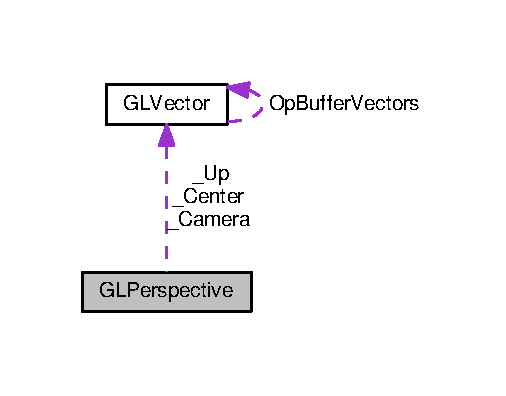
\includegraphics[width=243pt]{de/d2d/classGLPerspective__coll__graph}
\end{center}
\end{figure}
\subsection*{\-Public \-Member \-Functions}
\begin{DoxyCompactItemize}
\item 
\hyperlink{classGLPerspective_a7776461d3c1f2003fec732fbd57f20be}{\-G\-L\-Perspective} ()
\item 
\hyperlink{classGLPerspective_ad0ca059d1aa3ab81ea0de1286987a7a9}{$\sim$\-G\-L\-Perspective} ()
\item 
void \hyperlink{classGLPerspective_a91531aa2c2fab0c53a49c0fac32aac56}{apply} ()
\item 
void \hyperlink{classGLPerspective_a5a550ad5da6b057ee9dc30f50dde73b8}{turn\-Camera\-Up\-Down} (double angle\-Increment)
\item 
void \hyperlink{classGLPerspective_a7f2fb7087aff9d9b52a8cad0278e84df}{turn\-Camera\-Left\-Right} (double angle\-Increment)
\item 
void \hyperlink{classGLPerspective_a1faea9b30c847b83e52071f24f168a96}{stretch\-Camera\-Distance} (double factor)
\item 
void \hyperlink{classGLPerspective_abc3d6d9327be0c05122cfdfbbb35ae8b}{shift\-Scene\-Up\-Down} (double distance)
\item 
void \hyperlink{classGLPerspective_a15792e2d5f44be8e55bfe4be05220cec}{shift\-Scene\-Left\-Right} (double distance)
\item 
void \hyperlink{classGLPerspective_adac0de0074901f4896f5aaa19373c125}{shift\-Scene\-Forward\-Backward} (double distance)
\item 
void \hyperlink{classGLPerspective_afcdc1500b78321e8f7c172f16b5bb2cd}{set\-Camera} (const \hyperlink{classGLVector}{\-G\-L\-Vector} \&new\-Value)
\item 
void \hyperlink{classGLPerspective_acb39c3e367290da03409361ca42eded9}{set\-Center} (const \hyperlink{classGLVector}{\-G\-L\-Vector} \&new\-Value)
\item 
void \hyperlink{classGLPerspective_a09dd20fedcbc65dc790d1b50c0f94406}{set\-Up} (const \hyperlink{classGLVector}{\-G\-L\-Vector} \&new\-Value)
\item 
void \hyperlink{classGLPerspective_add4215ff5413bd2bf99cd769fc562045}{set\-Aspect} (\-G\-Ldouble new\-Value)
\item 
void \hyperlink{classGLPerspective_a95858a021bcceddd43d1df6822a0ce8d}{set\-Far} (\-G\-Ldouble new\-Value)
\item 
void \hyperlink{classGLPerspective_a585dc3dbb851d1dc2e751879362f8d7d}{set\-Fovy} (\-G\-Ldouble new\-Value)
\item 
void \hyperlink{classGLPerspective_a76c28c1b8d68d0c201c4dfadfd8863be}{set\-Near} (\-G\-Ldouble new\-Value)
\item 
void \hyperlink{classGLPerspective_a2269d593fd75d129c1b695b866afc6d1}{set\-Viewport} (int width, int height)
\item 
double \hyperlink{classGLPerspective_a5052aedb9d61e12e7499040608918a10}{distance} () const 
\end{DoxyCompactItemize}
\subsection*{\-Protected \-Attributes}
\begin{DoxyCompactItemize}
\item 
\hyperlink{classGLVector}{\-G\-L\-Vector} \hyperlink{classGLPerspective_a2bb94077d185cb85461a7c0eb53ab334}{\-\_\-\-Camera}
\item 
\hyperlink{classGLVector}{\-G\-L\-Vector} \hyperlink{classGLPerspective_acee62098421f0b59a62b1637f6ba586f}{\-\_\-\-Center}
\item 
\hyperlink{classGLVector}{\-G\-L\-Vector} \hyperlink{classGLPerspective_a69c80f817c645be3adc602e0adaf036c}{\-\_\-\-Up}
\item 
\-G\-Ldouble \hyperlink{classGLPerspective_a7355a44ee8fc58dedd79904ebe3093cb}{\-\_\-\-Aspect}
\item 
\-G\-Ldouble \hyperlink{classGLPerspective_a73b5c97c5d9b4c138eeeeff904c7ca57}{\-\_\-\-Far}
\item 
\-G\-Ldouble \hyperlink{classGLPerspective_a54617fb0638ba31e316b61c3dfb83c96}{\-\_\-\-Fovy}
\item 
\-G\-Ldouble \hyperlink{classGLPerspective_a7d6f75d52248d480136e8be881e9d4e6}{\-\_\-\-Near}
\item 
\-G\-Lint \hyperlink{classGLPerspective_a53d38f9b18e35f1d669c72e5c00a8f85}{\-\_\-\-Width}
\item 
\-G\-Lint \hyperlink{classGLPerspective_a6e4c1f9b9e2d2f98edfc6657e5b23a0f}{\-\_\-\-Height}
\end{DoxyCompactItemize}


\subsection{\-Detailed \-Description}
\-A class for encapsulating all data for a glu\-Perspective and a glu\-Look\-At call. \-These include\-: \-\_\-\-Fovy\-: \-Opening angle of frustum in y-\/direction (45° is a good average to start with) \-\_\-\-Aspect\-: \-The aspect ratio of the viewport (width / height) \-\_\-\-Near and \-\_\-\-Far clipping plane distances \-\_\-\-Center\-: \-The 3d-\/point to appear in the center of the viewport \-\_\-\-Camera\-: \-The 3d-\/point where the camera is \-\_\-\-Up\-: \-The 3d-\/vector that points upwards in the viewport

\-Use the \hyperlink{classGLPerspective_a91531aa2c2fab0c53a49c0fac32aac56}{apply()} function to transfer the perspective settings to the \-Open\-G\-L matrices.

\begin{DoxyAuthor}{\-Author}
walter $<$walter-\/\-Roth$>$ 
\end{DoxyAuthor}


\subsection{\-Constructor \& \-Destructor \-Documentation}
\hypertarget{classGLPerspective_a7776461d3c1f2003fec732fbd57f20be}{
\index{\-G\-L\-Perspective@{\-G\-L\-Perspective}!\-G\-L\-Perspective@{\-G\-L\-Perspective}}
\index{\-G\-L\-Perspective@{\-G\-L\-Perspective}!GLPerspective@{\-G\-L\-Perspective}}
\subsubsection[{\-G\-L\-Perspective}]{\setlength{\rightskip}{0pt plus 5cm}\-G\-L\-Perspective\-::\-G\-L\-Perspective (
\begin{DoxyParamCaption}
{}
\end{DoxyParamCaption}
)}}
\label{d1/d8f/classGLPerspective_a7776461d3c1f2003fec732fbd57f20be}

\begin{DoxyCode}
{
  _Center = v_Zero;
  _Camera = 5.0 * v_XYZ;
  _Up = v_Y;
  _Fovy = 45.0;
  _Aspect = 1.0;
  _Near = 1.0;
  _Far = 100000.0;
}
\end{DoxyCode}
\hypertarget{classGLPerspective_ad0ca059d1aa3ab81ea0de1286987a7a9}{
\index{\-G\-L\-Perspective@{\-G\-L\-Perspective}!$\sim$\-G\-L\-Perspective@{$\sim$\-G\-L\-Perspective}}
\index{$\sim$\-G\-L\-Perspective@{$\sim$\-G\-L\-Perspective}!GLPerspective@{\-G\-L\-Perspective}}
\subsubsection[{$\sim$\-G\-L\-Perspective}]{\setlength{\rightskip}{0pt plus 5cm}\-G\-L\-Perspective\-::$\sim$\-G\-L\-Perspective (
\begin{DoxyParamCaption}
{}
\end{DoxyParamCaption}
)}}
\label{d1/d8f/classGLPerspective_ad0ca059d1aa3ab81ea0de1286987a7a9}

\begin{DoxyCode}
{
}
\end{DoxyCode}


\subsection{\-Member \-Function \-Documentation}
\hypertarget{classGLPerspective_a91531aa2c2fab0c53a49c0fac32aac56}{
\index{\-G\-L\-Perspective@{\-G\-L\-Perspective}!apply@{apply}}
\index{apply@{apply}!GLPerspective@{\-G\-L\-Perspective}}
\subsubsection[{apply}]{\setlength{\rightskip}{0pt plus 5cm}void \-G\-L\-Perspective\-::apply (
\begin{DoxyParamCaption}
{}
\end{DoxyParamCaption}
)}}
\label{d1/d8f/classGLPerspective_a91531aa2c2fab0c53a49c0fac32aac56}
\-Applies the perspective settings to projection and modelview matrices. \-Old matrix values will be overwritten. \-To be called once before rendering the scene. 
\begin{DoxyCode}
                         {
  glMatrixMode(GL_PROJECTION); //switch to projection matrix
  glLoadIdentity();            //initialize matrix with identity matrix
  //multipy perspective transformation on projection matrix
  gluPerspective(_Fovy,    //fovy
                 _Aspect, //aspect
                 _Near,    //near
                 _Far);  //far

  glMatrixMode(GL_MODELVIEW);
  glLoadIdentity();
  gluLookAt(_Camera.x(), _Camera.y(), _Camera.z(), //eye
            _Center.x(), _Center.y(), _Center.z(),  //center
            _Up.x(), _Up.y(), _Up.z()); //up
} 
\end{DoxyCode}
\hypertarget{classGLPerspective_a5052aedb9d61e12e7499040608918a10}{
\index{\-G\-L\-Perspective@{\-G\-L\-Perspective}!distance@{distance}}
\index{distance@{distance}!GLPerspective@{\-G\-L\-Perspective}}
\subsubsection[{distance}]{\setlength{\rightskip}{0pt plus 5cm}double \-G\-L\-Perspective\-::distance (
\begin{DoxyParamCaption}
{}
\end{DoxyParamCaption}
) const\hspace{0.3cm}{\ttfamily  \mbox{[}inline\mbox{]}}}}
\label{d1/d8f/classGLPerspective_a5052aedb9d61e12e7499040608918a10}
\-Getters 
\begin{DoxyCode}
{ return (_Camera - _Center).length(); }
\end{DoxyCode}
\hypertarget{classGLPerspective_add4215ff5413bd2bf99cd769fc562045}{
\index{\-G\-L\-Perspective@{\-G\-L\-Perspective}!set\-Aspect@{set\-Aspect}}
\index{set\-Aspect@{set\-Aspect}!GLPerspective@{\-G\-L\-Perspective}}
\subsubsection[{set\-Aspect}]{\setlength{\rightskip}{0pt plus 5cm}void \-G\-L\-Perspective\-::set\-Aspect (
\begin{DoxyParamCaption}
\item[{\-G\-Ldouble}]{new\-Value}
\end{DoxyParamCaption}
)}}
\label{d1/d8f/classGLPerspective_add4215ff5413bd2bf99cd769fc562045}

\begin{DoxyCode}
                                              {
  _Aspect = newValue;
}
\end{DoxyCode}
\hypertarget{classGLPerspective_afcdc1500b78321e8f7c172f16b5bb2cd}{
\index{\-G\-L\-Perspective@{\-G\-L\-Perspective}!set\-Camera@{set\-Camera}}
\index{set\-Camera@{set\-Camera}!GLPerspective@{\-G\-L\-Perspective}}
\subsubsection[{set\-Camera}]{\setlength{\rightskip}{0pt plus 5cm}void \-G\-L\-Perspective\-::set\-Camera (
\begin{DoxyParamCaption}
\item[{const {\bf \-G\-L\-Vector} \&}]{new\-Value}
\end{DoxyParamCaption}
)}}
\label{d1/d8f/classGLPerspective_afcdc1500b78321e8f7c172f16b5bb2cd}
\-Setters 
\begin{DoxyCode}
                                                      {
   _Camera = newValue;
}
\end{DoxyCode}
\hypertarget{classGLPerspective_acb39c3e367290da03409361ca42eded9}{
\index{\-G\-L\-Perspective@{\-G\-L\-Perspective}!set\-Center@{set\-Center}}
\index{set\-Center@{set\-Center}!GLPerspective@{\-G\-L\-Perspective}}
\subsubsection[{set\-Center}]{\setlength{\rightskip}{0pt plus 5cm}void \-G\-L\-Perspective\-::set\-Center (
\begin{DoxyParamCaption}
\item[{const {\bf \-G\-L\-Vector} \&}]{new\-Value}
\end{DoxyParamCaption}
)}}
\label{d1/d8f/classGLPerspective_acb39c3e367290da03409361ca42eded9}

\begin{DoxyCode}
                                                      {
 _Center = newValue;
}
\end{DoxyCode}
\hypertarget{classGLPerspective_a95858a021bcceddd43d1df6822a0ce8d}{
\index{\-G\-L\-Perspective@{\-G\-L\-Perspective}!set\-Far@{set\-Far}}
\index{set\-Far@{set\-Far}!GLPerspective@{\-G\-L\-Perspective}}
\subsubsection[{set\-Far}]{\setlength{\rightskip}{0pt plus 5cm}void \-G\-L\-Perspective\-::set\-Far (
\begin{DoxyParamCaption}
\item[{\-G\-Ldouble}]{new\-Value}
\end{DoxyParamCaption}
)}}
\label{d1/d8f/classGLPerspective_a95858a021bcceddd43d1df6822a0ce8d}

\begin{DoxyCode}
                                           {
 _Far = newValue;
}
\end{DoxyCode}
\hypertarget{classGLPerspective_a585dc3dbb851d1dc2e751879362f8d7d}{
\index{\-G\-L\-Perspective@{\-G\-L\-Perspective}!set\-Fovy@{set\-Fovy}}
\index{set\-Fovy@{set\-Fovy}!GLPerspective@{\-G\-L\-Perspective}}
\subsubsection[{set\-Fovy}]{\setlength{\rightskip}{0pt plus 5cm}void \-G\-L\-Perspective\-::set\-Fovy (
\begin{DoxyParamCaption}
\item[{\-G\-Ldouble}]{new\-Value}
\end{DoxyParamCaption}
)}}
\label{d1/d8f/classGLPerspective_a585dc3dbb851d1dc2e751879362f8d7d}

\begin{DoxyCode}
                                            {
 _Fovy = newValue;
}
\end{DoxyCode}
\hypertarget{classGLPerspective_a76c28c1b8d68d0c201c4dfadfd8863be}{
\index{\-G\-L\-Perspective@{\-G\-L\-Perspective}!set\-Near@{set\-Near}}
\index{set\-Near@{set\-Near}!GLPerspective@{\-G\-L\-Perspective}}
\subsubsection[{set\-Near}]{\setlength{\rightskip}{0pt plus 5cm}void \-G\-L\-Perspective\-::set\-Near (
\begin{DoxyParamCaption}
\item[{\-G\-Ldouble}]{new\-Value}
\end{DoxyParamCaption}
)}}
\label{d1/d8f/classGLPerspective_a76c28c1b8d68d0c201c4dfadfd8863be}

\begin{DoxyCode}
                                            {
 _Near = newValue;
}
\end{DoxyCode}
\hypertarget{classGLPerspective_a09dd20fedcbc65dc790d1b50c0f94406}{
\index{\-G\-L\-Perspective@{\-G\-L\-Perspective}!set\-Up@{set\-Up}}
\index{set\-Up@{set\-Up}!GLPerspective@{\-G\-L\-Perspective}}
\subsubsection[{set\-Up}]{\setlength{\rightskip}{0pt plus 5cm}void \-G\-L\-Perspective\-::set\-Up (
\begin{DoxyParamCaption}
\item[{const {\bf \-G\-L\-Vector} \&}]{new\-Value}
\end{DoxyParamCaption}
)}}
\label{d1/d8f/classGLPerspective_a09dd20fedcbc65dc790d1b50c0f94406}

\begin{DoxyCode}
                                                  {
 _Up = newValue;
}
\end{DoxyCode}
\hypertarget{classGLPerspective_a2269d593fd75d129c1b695b866afc6d1}{
\index{\-G\-L\-Perspective@{\-G\-L\-Perspective}!set\-Viewport@{set\-Viewport}}
\index{set\-Viewport@{set\-Viewport}!GLPerspective@{\-G\-L\-Perspective}}
\subsubsection[{set\-Viewport}]{\setlength{\rightskip}{0pt plus 5cm}void \-G\-L\-Perspective\-::set\-Viewport (
\begin{DoxyParamCaption}
\item[{int}]{width, }
\item[{int}]{height}
\end{DoxyParamCaption}
)}}
\label{d1/d8f/classGLPerspective_a2269d593fd75d129c1b695b866afc6d1}
\-Sets viewport and adjusts \-\_\-\-Aspect to new viewport 
\begin{DoxyCode}
                                                    {
  _Width = width;
  _Height = height;
  glViewport(0,0, _Width, _Height);
  _Aspect = (double)_Width / (double)_Height;
}
\end{DoxyCode}
\hypertarget{classGLPerspective_adac0de0074901f4896f5aaa19373c125}{
\index{\-G\-L\-Perspective@{\-G\-L\-Perspective}!shift\-Scene\-Forward\-Backward@{shift\-Scene\-Forward\-Backward}}
\index{shift\-Scene\-Forward\-Backward@{shift\-Scene\-Forward\-Backward}!GLPerspective@{\-G\-L\-Perspective}}
\subsubsection[{shift\-Scene\-Forward\-Backward}]{\setlength{\rightskip}{0pt plus 5cm}void \-G\-L\-Perspective\-::shift\-Scene\-Forward\-Backward (
\begin{DoxyParamCaption}
\item[{double}]{distance}
\end{DoxyParamCaption}
)}}
\label{d1/d8f/classGLPerspective_adac0de0074901f4896f5aaa19373c125}
\-Shift the whole scene in x-\/z plane parallel to camera vector projection in xz plane 
\begin{DoxyCode}
{
 GLVector vShift = GLVector(_Center.x() -_Camera.x(), _Center.y() -_Camera.y(),
       0).unitVector() * distance;
 _Center = _Center + vShift;
 _Camera = _Camera + vShift; 
}
\end{DoxyCode}
\hypertarget{classGLPerspective_a15792e2d5f44be8e55bfe4be05220cec}{
\index{\-G\-L\-Perspective@{\-G\-L\-Perspective}!shift\-Scene\-Left\-Right@{shift\-Scene\-Left\-Right}}
\index{shift\-Scene\-Left\-Right@{shift\-Scene\-Left\-Right}!GLPerspective@{\-G\-L\-Perspective}}
\subsubsection[{shift\-Scene\-Left\-Right}]{\setlength{\rightskip}{0pt plus 5cm}void \-G\-L\-Perspective\-::shift\-Scene\-Left\-Right (
\begin{DoxyParamCaption}
\item[{double}]{distance}
\end{DoxyParamCaption}
)}}
\label{d1/d8f/classGLPerspective_a15792e2d5f44be8e55bfe4be05220cec}
\-Shift the whole scene in x-\/z plane orthogonal to camera vector 
\begin{DoxyCode}
{
 GLVector vShift = (_Center - _Camera).normalVector(_Up) * distance;
 _Center = _Center + vShift;
 _Camera = _Camera + vShift; 
}
\end{DoxyCode}
\hypertarget{classGLPerspective_abc3d6d9327be0c05122cfdfbbb35ae8b}{
\index{\-G\-L\-Perspective@{\-G\-L\-Perspective}!shift\-Scene\-Up\-Down@{shift\-Scene\-Up\-Down}}
\index{shift\-Scene\-Up\-Down@{shift\-Scene\-Up\-Down}!GLPerspective@{\-G\-L\-Perspective}}
\subsubsection[{shift\-Scene\-Up\-Down}]{\setlength{\rightskip}{0pt plus 5cm}void \-G\-L\-Perspective\-::shift\-Scene\-Up\-Down (
\begin{DoxyParamCaption}
\item[{double}]{distance}
\end{DoxyParamCaption}
)}}
\label{d1/d8f/classGLPerspective_abc3d6d9327be0c05122cfdfbbb35ae8b}
\-Shift the whole scene in y direction 
\begin{DoxyCode}
{
 GLVector vShift = distance * _Up;
 _Center = _Center + vShift;
 _Camera = _Camera + vShift;
}
\end{DoxyCode}
\hypertarget{classGLPerspective_a1faea9b30c847b83e52071f24f168a96}{
\index{\-G\-L\-Perspective@{\-G\-L\-Perspective}!stretch\-Camera\-Distance@{stretch\-Camera\-Distance}}
\index{stretch\-Camera\-Distance@{stretch\-Camera\-Distance}!GLPerspective@{\-G\-L\-Perspective}}
\subsubsection[{stretch\-Camera\-Distance}]{\setlength{\rightskip}{0pt plus 5cm}void \-G\-L\-Perspective\-::stretch\-Camera\-Distance (
\begin{DoxyParamCaption}
\item[{double}]{factor}
\end{DoxyParamCaption}
)}}
\label{d1/d8f/classGLPerspective_a1faea9b30c847b83e52071f24f168a96}
\-Multiply camera vector by factor 
\begin{DoxyCode}
{
  GLVector dist = _Camera - _Center;
  dist = dist * factor;
  setCamera(_Center + dist); 
}
\end{DoxyCode}
\hypertarget{classGLPerspective_a7f2fb7087aff9d9b52a8cad0278e84df}{
\index{\-G\-L\-Perspective@{\-G\-L\-Perspective}!turn\-Camera\-Left\-Right@{turn\-Camera\-Left\-Right}}
\index{turn\-Camera\-Left\-Right@{turn\-Camera\-Left\-Right}!GLPerspective@{\-G\-L\-Perspective}}
\subsubsection[{turn\-Camera\-Left\-Right}]{\setlength{\rightskip}{0pt plus 5cm}void \-G\-L\-Perspective\-::turn\-Camera\-Left\-Right (
\begin{DoxyParamCaption}
\item[{double}]{angle\-Increment}
\end{DoxyParamCaption}
)}}
\label{d1/d8f/classGLPerspective_a7f2fb7087aff9d9b52a8cad0278e84df}
\-Moves the camera on a latitude without modifying the distance to \-\_\-\-Center \-Maximum angle is +180 (east), minimum is -\/180 (west) 
\begin{DoxyCode}
                                                             {
  double radius, longitude, latitude;
  GLVector dist = _Camera - _Center;
  radius= dist.length();
  longitude = dist.longitude() + angleIncrement;
  if(longitude > 180.0)
   longitude -= 360.0;
  if (longitude < -180.0)
   longitude += 360.0;
  latitude = dist.latitude();
  dist.setRadiusLongitudeLatitude(radius, longitude,latitude);
  setCamera(_Center + dist); 
}
\end{DoxyCode}
\hypertarget{classGLPerspective_a5a550ad5da6b057ee9dc30f50dde73b8}{
\index{\-G\-L\-Perspective@{\-G\-L\-Perspective}!turn\-Camera\-Up\-Down@{turn\-Camera\-Up\-Down}}
\index{turn\-Camera\-Up\-Down@{turn\-Camera\-Up\-Down}!GLPerspective@{\-G\-L\-Perspective}}
\subsubsection[{turn\-Camera\-Up\-Down}]{\setlength{\rightskip}{0pt plus 5cm}void \-G\-L\-Perspective\-::turn\-Camera\-Up\-Down (
\begin{DoxyParamCaption}
\item[{double}]{angle\-Increment}
\end{DoxyParamCaption}
)}}
\label{d1/d8f/classGLPerspective_a5a550ad5da6b057ee9dc30f50dde73b8}
\-Moves the camera on a meridian without modifying the distance to \-\_\-\-Center \-Maximum angle is +90 (north), minimum is -\/90 (south) 
\begin{DoxyCode}
                                                            {
  double radius, longitude, latitude;
  GLVector dist = _Camera - _Center;
  radius= dist.length(); //use getters for coordinate transformation
  longitude = dist.longitude();
  latitude = dist.latitude() + angleIncrement;
  if(latitude > 90.0) //no flying over the poles
   latitude = 90.0;
  if (latitude < -90.0)
   latitude = -90.0;

  dist.setRadiusLongitudeLatitude(radius, longitude,latitude);
  setCamera(_Center + dist); //add dist to get new cam,era position
}
\end{DoxyCode}


\subsection{\-Member \-Data \-Documentation}
\hypertarget{classGLPerspective_a7355a44ee8fc58dedd79904ebe3093cb}{
\index{\-G\-L\-Perspective@{\-G\-L\-Perspective}!\-\_\-\-Aspect@{\-\_\-\-Aspect}}
\index{\-\_\-\-Aspect@{\-\_\-\-Aspect}!GLPerspective@{\-G\-L\-Perspective}}
\subsubsection[{\-\_\-\-Aspect}]{\setlength{\rightskip}{0pt plus 5cm}\-G\-Ldouble {\bf \-G\-L\-Perspective\-::\-\_\-\-Aspect}\hspace{0.3cm}{\ttfamily  \mbox{[}protected\mbox{]}}}}
\label{d1/d8f/classGLPerspective_a7355a44ee8fc58dedd79904ebe3093cb}
\hypertarget{classGLPerspective_a2bb94077d185cb85461a7c0eb53ab334}{
\index{\-G\-L\-Perspective@{\-G\-L\-Perspective}!\-\_\-\-Camera@{\-\_\-\-Camera}}
\index{\-\_\-\-Camera@{\-\_\-\-Camera}!GLPerspective@{\-G\-L\-Perspective}}
\subsubsection[{\-\_\-\-Camera}]{\setlength{\rightskip}{0pt plus 5cm}{\bf \-G\-L\-Vector} {\bf \-G\-L\-Perspective\-::\-\_\-\-Camera}\hspace{0.3cm}{\ttfamily  \mbox{[}protected\mbox{]}}}}
\label{d1/d8f/classGLPerspective_a2bb94077d185cb85461a7c0eb53ab334}
\hypertarget{classGLPerspective_acee62098421f0b59a62b1637f6ba586f}{
\index{\-G\-L\-Perspective@{\-G\-L\-Perspective}!\-\_\-\-Center@{\-\_\-\-Center}}
\index{\-\_\-\-Center@{\-\_\-\-Center}!GLPerspective@{\-G\-L\-Perspective}}
\subsubsection[{\-\_\-\-Center}]{\setlength{\rightskip}{0pt plus 5cm}{\bf \-G\-L\-Vector} {\bf \-G\-L\-Perspective\-::\-\_\-\-Center}\hspace{0.3cm}{\ttfamily  \mbox{[}protected\mbox{]}}}}
\label{d1/d8f/classGLPerspective_acee62098421f0b59a62b1637f6ba586f}
\hypertarget{classGLPerspective_a73b5c97c5d9b4c138eeeeff904c7ca57}{
\index{\-G\-L\-Perspective@{\-G\-L\-Perspective}!\-\_\-\-Far@{\-\_\-\-Far}}
\index{\-\_\-\-Far@{\-\_\-\-Far}!GLPerspective@{\-G\-L\-Perspective}}
\subsubsection[{\-\_\-\-Far}]{\setlength{\rightskip}{0pt plus 5cm}\-G\-Ldouble {\bf \-G\-L\-Perspective\-::\-\_\-\-Far}\hspace{0.3cm}{\ttfamily  \mbox{[}protected\mbox{]}}}}
\label{d1/d8f/classGLPerspective_a73b5c97c5d9b4c138eeeeff904c7ca57}
\hypertarget{classGLPerspective_a54617fb0638ba31e316b61c3dfb83c96}{
\index{\-G\-L\-Perspective@{\-G\-L\-Perspective}!\-\_\-\-Fovy@{\-\_\-\-Fovy}}
\index{\-\_\-\-Fovy@{\-\_\-\-Fovy}!GLPerspective@{\-G\-L\-Perspective}}
\subsubsection[{\-\_\-\-Fovy}]{\setlength{\rightskip}{0pt plus 5cm}\-G\-Ldouble {\bf \-G\-L\-Perspective\-::\-\_\-\-Fovy}\hspace{0.3cm}{\ttfamily  \mbox{[}protected\mbox{]}}}}
\label{d1/d8f/classGLPerspective_a54617fb0638ba31e316b61c3dfb83c96}
\hypertarget{classGLPerspective_a6e4c1f9b9e2d2f98edfc6657e5b23a0f}{
\index{\-G\-L\-Perspective@{\-G\-L\-Perspective}!\-\_\-\-Height@{\-\_\-\-Height}}
\index{\-\_\-\-Height@{\-\_\-\-Height}!GLPerspective@{\-G\-L\-Perspective}}
\subsubsection[{\-\_\-\-Height}]{\setlength{\rightskip}{0pt plus 5cm}\-G\-Lint {\bf \-G\-L\-Perspective\-::\-\_\-\-Height}\hspace{0.3cm}{\ttfamily  \mbox{[}protected\mbox{]}}}}
\label{d1/d8f/classGLPerspective_a6e4c1f9b9e2d2f98edfc6657e5b23a0f}
\-Viewport height \hypertarget{classGLPerspective_a7d6f75d52248d480136e8be881e9d4e6}{
\index{\-G\-L\-Perspective@{\-G\-L\-Perspective}!\-\_\-\-Near@{\-\_\-\-Near}}
\index{\-\_\-\-Near@{\-\_\-\-Near}!GLPerspective@{\-G\-L\-Perspective}}
\subsubsection[{\-\_\-\-Near}]{\setlength{\rightskip}{0pt plus 5cm}\-G\-Ldouble {\bf \-G\-L\-Perspective\-::\-\_\-\-Near}\hspace{0.3cm}{\ttfamily  \mbox{[}protected\mbox{]}}}}
\label{d1/d8f/classGLPerspective_a7d6f75d52248d480136e8be881e9d4e6}
\hypertarget{classGLPerspective_a69c80f817c645be3adc602e0adaf036c}{
\index{\-G\-L\-Perspective@{\-G\-L\-Perspective}!\-\_\-\-Up@{\-\_\-\-Up}}
\index{\-\_\-\-Up@{\-\_\-\-Up}!GLPerspective@{\-G\-L\-Perspective}}
\subsubsection[{\-\_\-\-Up}]{\setlength{\rightskip}{0pt plus 5cm}{\bf \-G\-L\-Vector} {\bf \-G\-L\-Perspective\-::\-\_\-\-Up}\hspace{0.3cm}{\ttfamily  \mbox{[}protected\mbox{]}}}}
\label{d1/d8f/classGLPerspective_a69c80f817c645be3adc602e0adaf036c}
\hypertarget{classGLPerspective_a53d38f9b18e35f1d669c72e5c00a8f85}{
\index{\-G\-L\-Perspective@{\-G\-L\-Perspective}!\-\_\-\-Width@{\-\_\-\-Width}}
\index{\-\_\-\-Width@{\-\_\-\-Width}!GLPerspective@{\-G\-L\-Perspective}}
\subsubsection[{\-\_\-\-Width}]{\setlength{\rightskip}{0pt plus 5cm}\-G\-Lint {\bf \-G\-L\-Perspective\-::\-\_\-\-Width}\hspace{0.3cm}{\ttfamily  \mbox{[}protected\mbox{]}}}}
\label{d1/d8f/classGLPerspective_a53d38f9b18e35f1d669c72e5c00a8f85}
\-Viewport width 

\-The documentation for this class was generated from the following files\-:\begin{DoxyCompactItemize}
\item 
\-Open\-G\-L/\hyperlink{glperspective_8h}{glperspective.\-h}\item 
\-Open\-G\-L/\hyperlink{glperspective_8cpp}{glperspective.\-cpp}\end{DoxyCompactItemize}

\section{\-G\-L\-Vector \-Class \-Reference}
\label{d4/db1/classGLVector}\index{\-G\-L\-Vector@{\-G\-L\-Vector}}


{\ttfamily \#include $<$glvector.\-h$>$}



\-Collaboration diagram for \-G\-L\-Vector\-:\nopagebreak
\begin{figure}[H]
\begin{center}
\leavevmode
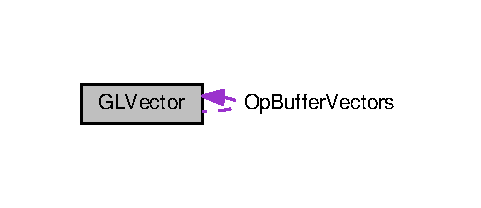
\includegraphics[width=231pt]{d7/d5b/classGLVector__coll__graph}
\end{center}
\end{figure}
\subsection*{\-Public \-Member \-Functions}
\begin{DoxyCompactItemize}
\item 
{\bf \-G\-L\-Vector} ()
\item 
{\bf $\sim$\-G\-L\-Vector} ()
\item 
{\bf \-G\-L\-Vector} (\-G\-Ldouble x, \-G\-Ldouble y, \-G\-Ldouble z)
\item 
{\bf \-G\-L\-Vector} (int angle\-Mode, \-G\-Ldouble radius, \-G\-Ldouble longitude, \-G\-Ldouble latitude)
\item 
{\bf \-G\-L\-Vector} (const {\bf \-G\-L\-Vector} \&to\-Copy)
\item 
\-G\-Ldouble {\bf x} () const 
\item 
void {\bf set\-X} (\-G\-Ldouble \-\_\-new\-Val)
\item 
\-G\-Ldouble {\bf y} () const 
\item 
void {\bf set\-Y} (\-G\-Ldouble \-\_\-new\-Val)
\item 
\-G\-Ldouble {\bf z} () const 
\item 
void {\bf set\-Z} (\-G\-Ldouble \-\_\-new\-Val)
\item 
const {\bf \-G\-L\-Vector} \& {\bf unit\-Vector} () const 
\item 
\-G\-Ldouble {\bf operator$\ast$} (const {\bf \-G\-L\-Vector} \&v2) const 
\item 
const {\bf \-G\-L\-Vector} \& {\bf vector\-Mult} (const {\bf \-G\-L\-Vector} \&v2) const 
\item 
const {\bf \-G\-L\-Vector} \& {\bf normal\-Vector} (const {\bf \-G\-L\-Vector} \&v2) const 
\item 
\-G\-Ldouble {\bf length} () const 
\item 
const {\bf \-G\-L\-Vector} {\bf rotate\-Vector} (const {\bf \-G\-L\-Vector} \&\-Axis, \-G\-Ldouble \-Angle) const 
\item 
const {\bf \-G\-L\-Vector} \& {\bf operator-\/} (const {\bf \-G\-L\-Vector} \&v2) const 
\item 
const {\bf \-G\-L\-Vector} \& {\bf operator+} (const {\bf \-G\-L\-Vector} \&v2) const 
\item 
\-G\-Ldouble $\ast$ {\bf dv} () const 
\item 
const {\bf \-G\-L\-Vector} \& {\bf stretch\-Vector} (\-G\-Ldouble sx, \-G\-Ldouble sy, \-G\-Ldouble sz) const 
\item 
const {\bf \-G\-L\-Vector} \& {\bf operator$\ast$} (\-G\-Ldouble f) const 
\item 
bool {\bf is\-Null} () const 
\item 
bool {\bf operator==} (const {\bf \-G\-L\-Vector} \&v2) const 
\item 
bool {\bf operator!=} (const {\bf \-G\-L\-Vector} \&v2) const 
\item 
{\bf \-G\-L\-Vector} \& {\bf operator=} (const {\bf \-G\-L\-Vector} \&to\-Copy)
\item 
const {\bf \-G\-L\-Vector} \& {\bf operator$\ast$} (const {\bf \-C\-G\-L\-Matrix} \&m) const 
\item 
\-Q\-String {\bf debug\-String} (const \-Q\-String \&caption) const 
\item 
void {\bf debug\-Output} (const \-Q\-String \&caption) const 
\item 
\-G\-Ldouble {\bf latitude} () const 
\item 
\-G\-Ldouble {\bf theta} () const 
\item 
\-G\-Ldouble {\bf radius} () const 
\item 
\-G\-Ldouble {\bf to\-Degree} (\-G\-Ldouble angle) const 
\item 
\-G\-Ldouble {\bf longitude} () const 
\item 
\-G\-Ldouble {\bf phi} () const 
\item 
const {\bf \-G\-L\-Vector} \& {\bf operator/} (\-G\-Ldouble f) const 
\item 
void {\bf set\-Radius\-Phi\-Theta} (\-G\-Ldouble radius, \-G\-Ldouble phi, \-G\-Ldouble theta)
\item 
void {\bf set\-Radius\-Longitude\-Latitude} (\-G\-Ldouble radius, \-G\-Ldouble longitude, \-G\-Ldouble latitude)
\item 
\-G\-Ldouble {\bf to\-Radian} (\-G\-Ldouble angle) const 
\item 
void {\bf vertex} () const 
\item 
\-G\-Ldouble {\bf scalar\-Mult} (const {\bf \-G\-L\-Vector} \&v2) const 
\item 
void {\bf limit\-To} (const {\bf \-G\-L\-Vector} \&min, const {\bf \-G\-L\-Vector} \&max)
\end{DoxyCompactItemize}
\subsection*{\-Static \-Public \-Member \-Functions}
\begin{DoxyCompactItemize}
\item 
static void {\bf debug\-Output\-Statistics} ()
\item 
static void {\bf set\-Angle\-Mode} (const int \&\-\_\-new\-Val)
\item 
static const int \& {\bf angle\-Mode} ()
\item 
static void {\bf debug\-Reset\-Counters} ()
\end{DoxyCompactItemize}
\subsection*{\-Static \-Public \-Attributes}
\begin{DoxyCompactItemize}
\item 
static const int {\bf \-Use360\-Degree} = 1
\item 
static const int {\bf \-Use400\-New\-Degree} = 2
\item 
static const int {\bf \-Use\-Radian} = 3
\item 
static const int {\bf \-Available\-Op\-Buffers} = 3
\end{DoxyCompactItemize}
\subsection*{\-Protected \-Member \-Functions}
\begin{DoxyCompactItemize}
\item 
void {\bf copy} (const {\bf \-G\-L\-Vector} \&to\-Copy)
\end{DoxyCompactItemize}
\subsection*{\-Static \-Protected \-Member \-Functions}
\begin{DoxyCompactItemize}
\item 
static const {\bf \-G\-L\-Vector} \& {\bf next\-Buffer} (\-G\-Ldouble x, \-G\-Ldouble y, \-G\-Ldouble z)
\end{DoxyCompactItemize}
\subsection*{\-Protected \-Attributes}
\begin{DoxyCompactItemize}
\item 
\-G\-Ldouble {\bfseries \-\_\-\-X}\label{d4/db1/classGLVector_a9450f309bf0b64245937f36606a3489f}

\item 
\-G\-Ldouble {\bfseries \-\_\-\-Y}\label{d4/db1/classGLVector_a638c2f737d3fce449d64e5aae5b15aa8}

\item 
\-G\-Ldouble {\bfseries \-\_\-\-Z}\label{d4/db1/classGLVector_a95097d48b78403b59733b95ac857656a}

\end{DoxyCompactItemize}
\subsection*{\-Static \-Protected \-Attributes}
\begin{DoxyCompactItemize}
\item 
static int {\bf \-\_\-\-Angle\-Mode} = {\bf \-G\-L\-Vector\-::\-Use360\-Degree}
\item 
static {\bf \-G\-L\-Vector} {\bf \-Op\-Buffer\-Vectors} [{\bf \-Available\-Op\-Buffers}]
\item 
static int {\bf n\-\_\-\-Buffer} = 0
\item 
static int {\bf n\-\_\-\-Max\-Buffers} = 0
\item 
static int {\bf n\-\_\-\-Operator\-Calls} = 0
\item 
static int {\bf n\-\_\-\-Copy\-Calls} = 0
\item 
static int {\bf n\-\_\-\-Constructor\-Calls} = 0
\item 
static int {\bf n\-\_\-\-Vertex\-Calls} = 0
\end{DoxyCompactItemize}


\subsection{\-Detailed \-Description}
\-A vector with 3 dimensions in \-G\-Ldouble numbers, especially designed for use with \-Open\-G\-L. \-Can be used easily with \-G\-L\-\_\-xxx3dv functions. \-Use the \doxyref{dv()}{p.}{d4/db1/classGLVector_a3408513f72b99c63c81702f2e2ccba96} member function to obtain a \-G\-Ldouble $\ast$ to the data. \-Alternatively, you may use \doxyref{vertex()}{p.}{d4/db1/classGLVector_a050ef5239fb7a6d83ef5158c955fa006} for calls to gl\-Vertex and normal() for calls to gl\-Normal. \-Contains the basic vector maths as memberfunctions and operators. \-May be used with cartesian (x, y, z), geographic (radius, longitude angle counterclockwise around y axis starting at z axis and latitude angle from equatorial xz plane up and down 90) and polar coordinates ( radius, phi angle around z axis counterclockwise from x axis, theta angle from positive z axis downwards). \-Radius is the length of the vector. \-All angle functions work with 360 degree angles, unless you set \doxyref{\-G\-L\-Vector\-::\-Use\-Radian}{p.}{d4/db1/classGLVector_a8b1fc370c56a13540109b9b6f3d4f5df} or \doxyref{\-G\-L\-Vector\-::\-Use400\-New\-Degree}{p.}{d4/db1/classGLVector_a4ee1d6d06257b4e5399ad196eb6db536} with the set\-Angle\-Mode class function. \-However, there is a constructor for geographic coordinates with a local \-Angle\-Mode, that accepts geographic coordinates and radian, 360 degree or 400 new degree angle values. \-Pass \-Use360\-Degree or \-Use400\-New\-Degree as first parameter, if you want to use degrees. \-For polar coordinates, use the set\-Radius\-Phi\-Theta function. \-Data are kept as cartesian coordinates internally. \-Therefore, the geographic and polar values may have rounding errors in the order of 10\-E-\/13. \-All calculation functions except those operators, that include a = (=, +=, $\ast$= ...) are const functions. \-This means, if you want to rotate a vector foo itself, you have to call\-: foo = foo.\-rotate\-Vector(). \-For convenience, there are a couple of predefined vectors at the end of this header file (v\-\_\-\-X, v\-\_\-\-Y..).

\-This class is designed for high performance and not for subclassing. \-Undefine \-D\-E\-B\-U\-G\-\_\-\-G\-L\-V\-E\-C\-T\-O\-R for maximum performance (refer to top of header file). \-There are no virtual functions, which would create a \-V\-M\-T. \-This increases performance. \-Make functions virtual, if you want to subclass (\-N\-O\-T recommended). \-The operators return references to members of the protected \-Op\-Buffer\-Vectors array. \-This avoids permanent construction and destruction of temporary \-G\-L\-Vectors for calculation results.{\bfseries  \-The predefined maximum number of nested calculations is 32. \-If you need more, increase the value of \-Available\-Op\-Buffers. \-See the get\-Next\-Buffer function for details. \-Use \doxyref{debug\-Output\-Statistics()}{p.}{d4/db1/classGLVector_add2a39dc176e05b68c02375fb674820e} to obtain informations on buffer useage and call statistics. \-Operator buffer overflow is very likely, if results of vector calculations are passed as reference parameters to functions that perform lots of calculations. \-In these cases use \char`\"{}call by value\char`\"{} parameters or make an explicit copy of the reference parameter. } \begin{DoxyAuthor}{\-Author}
\-Walter \-Roth 
\end{DoxyAuthor}


\subsection{\-Constructor \& \-Destructor \-Documentation}
\index{\-G\-L\-Vector@{\-G\-L\-Vector}!\-G\-L\-Vector@{\-G\-L\-Vector}}
\index{\-G\-L\-Vector@{\-G\-L\-Vector}!GLVector@{\-G\-L\-Vector}}
\subsubsection[{\-G\-L\-Vector}]{\setlength{\rightskip}{0pt plus 5cm}\-G\-L\-Vector\-::\-G\-L\-Vector (
\begin{DoxyParamCaption}
{}
\end{DoxyParamCaption}
)}\label{d4/db1/classGLVector_ac747e4f072b314baeb6decc743ed1641}
\-Standard constructor, creates a zero vector \index{\-G\-L\-Vector@{\-G\-L\-Vector}!$\sim$\-G\-L\-Vector@{$\sim$\-G\-L\-Vector}}
\index{$\sim$\-G\-L\-Vector@{$\sim$\-G\-L\-Vector}!GLVector@{\-G\-L\-Vector}}
\subsubsection[{$\sim$\-G\-L\-Vector}]{\setlength{\rightskip}{0pt plus 5cm}\-G\-L\-Vector\-::$\sim$\-G\-L\-Vector (
\begin{DoxyParamCaption}
{}
\end{DoxyParamCaption}
)}\label{d4/db1/classGLVector_ae2e7538b0fcd843aa8cb6fabbe28cd57}
\-Destructor, presently it does nothing. \index{\-G\-L\-Vector@{\-G\-L\-Vector}!\-G\-L\-Vector@{\-G\-L\-Vector}}
\index{\-G\-L\-Vector@{\-G\-L\-Vector}!GLVector@{\-G\-L\-Vector}}
\subsubsection[{\-G\-L\-Vector}]{\setlength{\rightskip}{0pt plus 5cm}\-G\-L\-Vector\-::\-G\-L\-Vector (
\begin{DoxyParamCaption}
\item[{\-G\-Ldouble}]{x, }
\item[{\-G\-Ldouble}]{y, }
\item[{\-G\-Ldouble}]{z}
\end{DoxyParamCaption}
)}\label{d4/db1/classGLVector_a1516a07954fdfa30ebb24813f3967df1}
\-Constructor for cartesian coordinates. \index{\-G\-L\-Vector@{\-G\-L\-Vector}!\-G\-L\-Vector@{\-G\-L\-Vector}}
\index{\-G\-L\-Vector@{\-G\-L\-Vector}!GLVector@{\-G\-L\-Vector}}
\subsubsection[{\-G\-L\-Vector}]{\setlength{\rightskip}{0pt plus 5cm}\-G\-L\-Vector\-::\-G\-L\-Vector (
\begin{DoxyParamCaption}
\item[{int}]{angle\-Mode, }
\item[{\-G\-Ldouble}]{radius, }
\item[{\-G\-Ldouble}]{longitude, }
\item[{\-G\-Ldouble}]{latitude}
\end{DoxyParamCaption}
)}\label{d4/db1/classGLVector_a2ec6b7a49e5432b1a02a3ab812ea23ae}
\-Constructor for geographic coordinates. \-Pass \-Use\-Radian, \-Use360\-Degree or \-Use400\-New\-Degree as value for angle\-Mode. \-Static \-Angle\-Mode is \-N\-O\-T affected. \-Alternatives\-: \-Construct a \doxyref{\-G\-L\-Vector}{p.}{d4/db1/classGLVector} using the standard constructor. \-Then call set\-Radius\-Phi\-Theta for polar or set\-Radius\-Longitude\-Latitude for geographic coordinates.

\-Constructor for polar coordinates. \-Pass \-Use\-Radian, \-Use360\-Degree or \-Use400\-New\-Degree as value for angle\-Mode. \index{\-G\-L\-Vector@{\-G\-L\-Vector}!\-G\-L\-Vector@{\-G\-L\-Vector}}
\index{\-G\-L\-Vector@{\-G\-L\-Vector}!GLVector@{\-G\-L\-Vector}}
\subsubsection[{\-G\-L\-Vector}]{\setlength{\rightskip}{0pt plus 5cm}\-G\-L\-Vector\-::\-G\-L\-Vector (
\begin{DoxyParamCaption}
\item[{const {\bf \-G\-L\-Vector} \&}]{to\-Copy}
\end{DoxyParamCaption}
)}\label{d4/db1/classGLVector_a64ca3d25c4c8816232404e9f26f0bc12}
\-Copy constructor. \-Calls \doxyref{copy()}{p.}{d4/db1/classGLVector_a61f9f40992082292e73190c59b1f95cd} function. 

\subsection{\-Member \-Function \-Documentation}
\index{\-G\-L\-Vector@{\-G\-L\-Vector}!angle\-Mode@{angle\-Mode}}
\index{angle\-Mode@{angle\-Mode}!GLVector@{\-G\-L\-Vector}}
\subsubsection[{angle\-Mode}]{\setlength{\rightskip}{0pt plus 5cm}const int \& \-G\-L\-Vector\-::angle\-Mode (
\begin{DoxyParamCaption}
{}
\end{DoxyParamCaption}
)\hspace{0.3cm}{\ttfamily  [static]}}\label{d4/db1/classGLVector_ab697a8814c499f9924c9340d74f02e12}
\-Read property of int \-\_\-\-Angle\-Mode. \index{\-G\-L\-Vector@{\-G\-L\-Vector}!copy@{copy}}
\index{copy@{copy}!GLVector@{\-G\-L\-Vector}}
\subsubsection[{copy}]{\setlength{\rightskip}{0pt plus 5cm}void \-G\-L\-Vector\-::copy (
\begin{DoxyParamCaption}
\item[{const {\bf \-G\-L\-Vector} \&}]{to\-Copy}
\end{DoxyParamCaption}
)\hspace{0.3cm}{\ttfamily  [protected]}}\label{d4/db1/classGLVector_a61f9f40992082292e73190c59b1f95cd}
\-Copy function used by copy constructor and operator =. \index{\-G\-L\-Vector@{\-G\-L\-Vector}!debug\-Output@{debug\-Output}}
\index{debug\-Output@{debug\-Output}!GLVector@{\-G\-L\-Vector}}
\subsubsection[{debug\-Output}]{\setlength{\rightskip}{0pt plus 5cm}void \-G\-L\-Vector\-::debug\-Output (
\begin{DoxyParamCaption}
\item[{const \-Q\-String \&}]{caption}
\end{DoxyParamCaption}
) const}\label{d4/db1/classGLVector_acf794d36606266d0cf9a01564f6cb0ce}
\-Writes list of coordinates to stderr. \index{\-G\-L\-Vector@{\-G\-L\-Vector}!debug\-Output\-Statistics@{debug\-Output\-Statistics}}
\index{debug\-Output\-Statistics@{debug\-Output\-Statistics}!GLVector@{\-G\-L\-Vector}}
\subsubsection[{debug\-Output\-Statistics}]{\setlength{\rightskip}{0pt plus 5cm}void \-G\-L\-Vector\-::debug\-Output\-Statistics (
\begin{DoxyParamCaption}
{}
\end{DoxyParamCaption}
)\hspace{0.3cm}{\ttfamily  [static]}}\label{d4/db1/classGLVector_add2a39dc176e05b68c02375fb674820e}
\-Produces a debug output of the number of operations, constructor calls etc.

\-Produces a debug output of the number of operations, constructoir calls etc. \index{\-G\-L\-Vector@{\-G\-L\-Vector}!debug\-Reset\-Counters@{debug\-Reset\-Counters}}
\index{debug\-Reset\-Counters@{debug\-Reset\-Counters}!GLVector@{\-G\-L\-Vector}}
\subsubsection[{debug\-Reset\-Counters}]{\setlength{\rightskip}{0pt plus 5cm}void \-G\-L\-Vector\-::debug\-Reset\-Counters (
\begin{DoxyParamCaption}
{}
\end{DoxyParamCaption}
)\hspace{0.3cm}{\ttfamily  [static]}}\label{d4/db1/classGLVector_a7e54a0a197b0f4cab2b848fd7e9e74d8}
\-Sets debugging counters to 0. \index{\-G\-L\-Vector@{\-G\-L\-Vector}!debug\-String@{debug\-String}}
\index{debug\-String@{debug\-String}!GLVector@{\-G\-L\-Vector}}
\subsubsection[{debug\-String}]{\setlength{\rightskip}{0pt plus 5cm}\-Q\-String \-G\-L\-Vector\-::debug\-String (
\begin{DoxyParamCaption}
\item[{const \-Q\-String \&}]{caption}
\end{DoxyParamCaption}
) const}\label{d4/db1/classGLVector_a901db0ed0c94de90dc9ef3890f63a8f2}
\-Returns the debug output string. \index{\-G\-L\-Vector@{\-G\-L\-Vector}!dv@{dv}}
\index{dv@{dv}!GLVector@{\-G\-L\-Vector}}
\subsubsection[{dv}]{\setlength{\rightskip}{0pt plus 5cm}\-G\-Ldouble $\ast$ \-G\-L\-Vector\-::dv (
\begin{DoxyParamCaption}
{}
\end{DoxyParamCaption}
) const}\label{d4/db1/classGLVector_a3408513f72b99c63c81702f2e2ccba96}
\-For use with gl\-X\-X\-X\-X3dv functions. \-This function relies on the internal order of declaration.

\-For use with gl\-X\-X\-X\-X3dv functions. \index{\-G\-L\-Vector@{\-G\-L\-Vector}!is\-Null@{is\-Null}}
\index{is\-Null@{is\-Null}!GLVector@{\-G\-L\-Vector}}
\subsubsection[{is\-Null}]{\setlength{\rightskip}{0pt plus 5cm}bool \-G\-L\-Vector\-::is\-Null (
\begin{DoxyParamCaption}
{}
\end{DoxyParamCaption}
) const}\label{d4/db1/classGLVector_a5b14415969ab6c060ee232797e79d14f}
\-Returns true, if all coordinates are 0. \index{\-G\-L\-Vector@{\-G\-L\-Vector}!latitude@{latitude}}
\index{latitude@{latitude}!GLVector@{\-G\-L\-Vector}}
\subsubsection[{latitude}]{\setlength{\rightskip}{0pt plus 5cm}\-G\-Ldouble \-G\-L\-Vector\-::latitude (
\begin{DoxyParamCaption}
{}
\end{DoxyParamCaption}
) const}\label{d4/db1/classGLVector_a805eb8881b69be9dea3bbcd3a85ee9c6}
\-Returns latitude angle from equatorial xz plane up and down.

\-Returns latitude angle form equatorial xz plane up and down. \index{\-G\-L\-Vector@{\-G\-L\-Vector}!length@{length}}
\index{length@{length}!GLVector@{\-G\-L\-Vector}}
\subsubsection[{length}]{\setlength{\rightskip}{0pt plus 5cm}\-G\-Ldouble \-G\-L\-Vector\-::length (
\begin{DoxyParamCaption}
{}
\end{DoxyParamCaption}
) const}\label{d4/db1/classGLVector_a3574d0c6514a5de5838d6e487ec61408}
\-Caculates the length. \index{\-G\-L\-Vector@{\-G\-L\-Vector}!limit\-To@{limit\-To}}
\index{limit\-To@{limit\-To}!GLVector@{\-G\-L\-Vector}}
\subsubsection[{limit\-To}]{\setlength{\rightskip}{0pt plus 5cm}void \-G\-L\-Vector\-::limit\-To (
\begin{DoxyParamCaption}
\item[{const {\bf \-G\-L\-Vector} \&}]{min, }
\item[{const {\bf \-G\-L\-Vector} \&}]{max}
\end{DoxyParamCaption}
)}\label{d4/db1/classGLVector_a5b5cd462d5adab754f0936f63510fc66}
\-Limits coordinates to values between min and max. \index{\-G\-L\-Vector@{\-G\-L\-Vector}!longitude@{longitude}}
\index{longitude@{longitude}!GLVector@{\-G\-L\-Vector}}
\subsubsection[{longitude}]{\setlength{\rightskip}{0pt plus 5cm}\-G\-Ldouble \-G\-L\-Vector\-::longitude (
\begin{DoxyParamCaption}
{}
\end{DoxyParamCaption}
) const}\label{d4/db1/classGLVector_a0d7f20927c7d75d0aa240de15df89f5f}
\-Returns the longitude angle around y axis in radian, 360 degree or 400 new degree according to angle\-Mode. \-Angle starts at z-\/axis. \index{\-G\-L\-Vector@{\-G\-L\-Vector}!next\-Buffer@{next\-Buffer}}
\index{next\-Buffer@{next\-Buffer}!GLVector@{\-G\-L\-Vector}}
\subsubsection[{next\-Buffer}]{\setlength{\rightskip}{0pt plus 5cm}const {\bf \-G\-L\-Vector} \& \-G\-L\-Vector\-::next\-Buffer (
\begin{DoxyParamCaption}
\item[{\-G\-Ldouble}]{x, }
\item[{\-G\-Ldouble}]{y, }
\item[{\-G\-Ldouble}]{z}
\end{DoxyParamCaption}
)\hspace{0.3cm}{\ttfamily  [static, protected]}}\label{d4/db1/classGLVector_a5705bc9163f6d6a8f67ad8af7e5ef22c}
\-Copies x, y and z to the next (and hopefully free) buffer vector from the buffer ring \-Op\-Buffer\-Vectors and returns its address. \-The number of available buffer vectors is controlled by \-Available\-Op\-Buffer\-Vectors. {\bfseries \-There is no verification, whether a buffer position is no longer used. \-Therefore, if you are performing very deeply nested calculations, you may have to set \-Available\-Op\-Buffer\-Vectors to a higher value. \-Use \doxyref{debug\-Output\-Statistics()}{p.}{d4/db1/classGLVector_add2a39dc176e05b68c02375fb674820e} for debugging.}

\-Copies x, y and z to the next (and hopefully free) buffer vector from the buffer ring \-Op\-Buffer and returns its address. \-The number of available buffer vectors is controlled by \-Available\-Op\-Buffers. {\bfseries \-There is no verification, whether a buffer position is no longer used. \-Therefore, if you are performing very deeply nested calculations, you may have to set \-\_\-\-Buffer\-Vectors to a higher value.} \index{\-G\-L\-Vector@{\-G\-L\-Vector}!normal\-Vector@{normal\-Vector}}
\index{normal\-Vector@{normal\-Vector}!GLVector@{\-G\-L\-Vector}}
\subsubsection[{normal\-Vector}]{\setlength{\rightskip}{0pt plus 5cm}const {\bf \-G\-L\-Vector} \& \-G\-L\-Vector\-::normal\-Vector (
\begin{DoxyParamCaption}
\item[{const {\bf \-G\-L\-Vector} \&}]{v2}
\end{DoxyParamCaption}
) const}\label{d4/db1/classGLVector_a314b71f079b571846833a3beab71f7b0}
\-Normal vector with lenght 1.\-0 obtained by $\ast$this \-X v2.

\-Normal vector with length 1.\-0 obtained by $\ast$this \-X v2. \index{\-G\-L\-Vector@{\-G\-L\-Vector}!operator!=@{operator!=}}
\index{operator!=@{operator!=}!GLVector@{\-G\-L\-Vector}}
\subsubsection[{operator!=}]{\setlength{\rightskip}{0pt plus 5cm}bool \-G\-L\-Vector\-::operator!= (
\begin{DoxyParamCaption}
\item[{const {\bf \-G\-L\-Vector} \&}]{v2}
\end{DoxyParamCaption}
) const}\label{d4/db1/classGLVector_ab5edfaa1436322090272efd0e407a03a}
\-Compares two vectors. \-Uses !operator ==.

\-Compares two vectors. \index{\-G\-L\-Vector@{\-G\-L\-Vector}!operator$\ast$@{operator$\ast$}}
\index{operator$\ast$@{operator$\ast$}!GLVector@{\-G\-L\-Vector}}
\subsubsection[{operator$\ast$}]{\setlength{\rightskip}{0pt plus 5cm}\-G\-Ldouble \-G\-L\-Vector\-::operator$\ast$ (
\begin{DoxyParamCaption}
\item[{const {\bf \-G\-L\-Vector} \&}]{v2}
\end{DoxyParamCaption}
) const}\label{d4/db1/classGLVector_a4c2a156755e478e9ca5978ac603f9f47}
\-Scalar product. \-For vector product see function vector\-Mult.

\-Scalar product. \index{\-G\-L\-Vector@{\-G\-L\-Vector}!operator$\ast$@{operator$\ast$}}
\index{operator$\ast$@{operator$\ast$}!GLVector@{\-G\-L\-Vector}}
\subsubsection[{operator$\ast$}]{\setlength{\rightskip}{0pt plus 5cm}const {\bf \-G\-L\-Vector} \& \-G\-L\-Vector\-::operator$\ast$ (
\begin{DoxyParamCaption}
\item[{\-G\-Ldouble}]{f}
\end{DoxyParamCaption}
) const}\label{d4/db1/classGLVector_a3e9e3340cc0a39932462da5d2e92468d}
\-Multiplies vector with f. \index{\-G\-L\-Vector@{\-G\-L\-Vector}!operator$\ast$@{operator$\ast$}}
\index{operator$\ast$@{operator$\ast$}!GLVector@{\-G\-L\-Vector}}
\subsubsection[{operator$\ast$}]{\setlength{\rightskip}{0pt plus 5cm}const {\bf \-G\-L\-Vector} \& \-G\-L\-Vector\-::operator$\ast$ (
\begin{DoxyParamCaption}
\item[{const {\bf \-C\-G\-L\-Matrix} \&}]{m}
\end{DoxyParamCaption}
) const}\label{d4/db1/classGLVector_af188ad329ae3eca84fa87d77f4523428}
\-Multipies 3d \-Vector with 4$\ast$4 matrix. 4th coordinate of vector is assumed to be 1.\-0. \-Calculations run on main fpu. \-Use gl\-Mult\-Matrix for calculation on graphics processor. \index{\-G\-L\-Vector@{\-G\-L\-Vector}!operator+@{operator+}}
\index{operator+@{operator+}!GLVector@{\-G\-L\-Vector}}
\subsubsection[{operator+}]{\setlength{\rightskip}{0pt plus 5cm}const {\bf \-G\-L\-Vector} \& \-G\-L\-Vector\-::operator+ (
\begin{DoxyParamCaption}
\item[{const {\bf \-G\-L\-Vector} \&}]{v2}
\end{DoxyParamCaption}
) const}\label{d4/db1/classGLVector_a34942208c4b7c3a20bfc9b4e8a6b4ac5}
\-Returns the vectorsum of v1 and v2. \index{\-G\-L\-Vector@{\-G\-L\-Vector}!operator-\/@{operator-\/}}
\index{operator-\/@{operator-\/}!GLVector@{\-G\-L\-Vector}}
\subsubsection[{operator-\/}]{\setlength{\rightskip}{0pt plus 5cm}const {\bf \-G\-L\-Vector} \& \-G\-L\-Vector\-::operator-\/ (
\begin{DoxyParamCaption}
\item[{const {\bf \-G\-L\-Vector} \&}]{v2}
\end{DoxyParamCaption}
) const}\label{d4/db1/classGLVector_a05483ab1f6d777d33d681ee4fe3f6498}
\-Returns this -\/ v2. \index{\-G\-L\-Vector@{\-G\-L\-Vector}!operator/@{operator/}}
\index{operator/@{operator/}!GLVector@{\-G\-L\-Vector}}
\subsubsection[{operator/}]{\setlength{\rightskip}{0pt plus 5cm}const {\bf \-G\-L\-Vector} \& \-G\-L\-Vector\-::operator/ (
\begin{DoxyParamCaption}
\item[{\-G\-Ldouble}]{f}
\end{DoxyParamCaption}
) const}\label{d4/db1/classGLVector_aba1e99c3b11a7c30b446f609ae219295}
\-Multiplies vector with1/ f. \index{\-G\-L\-Vector@{\-G\-L\-Vector}!operator=@{operator=}}
\index{operator=@{operator=}!GLVector@{\-G\-L\-Vector}}
\subsubsection[{operator=}]{\setlength{\rightskip}{0pt plus 5cm}{\bf \-G\-L\-Vector} \& \-G\-L\-Vector\-::operator= (
\begin{DoxyParamCaption}
\item[{const {\bf \-G\-L\-Vector} \&}]{to\-Copy}
\end{DoxyParamCaption}
)}\label{d4/db1/classGLVector_ae0e364adbb7543f13c47cee12654ec69}
\-Copies to\-Copy and returns $\ast$ this. \index{\-G\-L\-Vector@{\-G\-L\-Vector}!operator==@{operator==}}
\index{operator==@{operator==}!GLVector@{\-G\-L\-Vector}}
\subsubsection[{operator==}]{\setlength{\rightskip}{0pt plus 5cm}bool \-G\-L\-Vector\-::operator== (
\begin{DoxyParamCaption}
\item[{const {\bf \-G\-L\-Vector} \&}]{v2}
\end{DoxyParamCaption}
) const}\label{d4/db1/classGLVector_ab95e61904b30cdae641a0c583548a557}
\-Compares two vectors. \-Will only return true if \-A\-L\-L digits of the \-G\-Ldouble coordinates are the same. \index{\-G\-L\-Vector@{\-G\-L\-Vector}!phi@{phi}}
\index{phi@{phi}!GLVector@{\-G\-L\-Vector}}
\subsubsection[{phi}]{\setlength{\rightskip}{0pt plus 5cm}\-G\-Ldouble \-G\-L\-Vector\-::phi (
\begin{DoxyParamCaption}
{}
\end{DoxyParamCaption}
) const}\label{d4/db1/classGLVector_afb2a8da7c9d50e05bac63d8ef5c4bdf3}
\-Returns phi angle around z axis in radian, 360 degree or 400 new degree according to angle\-Mode. \index{\-G\-L\-Vector@{\-G\-L\-Vector}!radius@{radius}}
\index{radius@{radius}!GLVector@{\-G\-L\-Vector}}
\subsubsection[{radius}]{\setlength{\rightskip}{0pt plus 5cm}\-G\-Ldouble \-G\-L\-Vector\-::radius (
\begin{DoxyParamCaption}
{}
\end{DoxyParamCaption}
) const}\label{d4/db1/classGLVector_abd8984744b5d57e4a7df0e7eb70b3fb1}
\-Returns length of vector, for convenience. \index{\-G\-L\-Vector@{\-G\-L\-Vector}!rotate\-Vector@{rotate\-Vector}}
\index{rotate\-Vector@{rotate\-Vector}!GLVector@{\-G\-L\-Vector}}
\subsubsection[{rotate\-Vector}]{\setlength{\rightskip}{0pt plus 5cm}const {\bf \-G\-L\-Vector} \-G\-L\-Vector\-::rotate\-Vector (
\begin{DoxyParamCaption}
\item[{const {\bf \-G\-L\-Vector} \&}]{\-Axis, }
\item[{\-G\-Ldouble}]{\-Angle}
\end{DoxyParamCaption}
) const}\label{d4/db1/classGLVector_aec8ac775e13b7ec0060198625d1ab747}
\-Returns a vector obtained by rotating $\ast$this around axis. \-Uses radian \-Angle. \index{\-G\-L\-Vector@{\-G\-L\-Vector}!scalar\-Mult@{scalar\-Mult}}
\index{scalar\-Mult@{scalar\-Mult}!GLVector@{\-G\-L\-Vector}}
\subsubsection[{scalar\-Mult}]{\setlength{\rightskip}{0pt plus 5cm}\-G\-Ldouble \-G\-L\-Vector\-::scalar\-Mult (
\begin{DoxyParamCaption}
\item[{const {\bf \-G\-L\-Vector} \&}]{v2}
\end{DoxyParamCaption}
) const}\label{d4/db1/classGLVector_a23499b64647ce6e3de2c633198deb78b}
\-Returns scalar product. \-May be used instead of operator $\ast$. \-For vector product see function vector\-Mult.

\-Returns scalar product. \index{\-G\-L\-Vector@{\-G\-L\-Vector}!set\-Angle\-Mode@{set\-Angle\-Mode}}
\index{set\-Angle\-Mode@{set\-Angle\-Mode}!GLVector@{\-G\-L\-Vector}}
\subsubsection[{set\-Angle\-Mode}]{\setlength{\rightskip}{0pt plus 5cm}void \-G\-L\-Vector\-::set\-Angle\-Mode (
\begin{DoxyParamCaption}
\item[{const int \&}]{\-\_\-new\-Val}
\end{DoxyParamCaption}
)\hspace{0.3cm}{\ttfamily  [static]}}\label{d4/db1/classGLVector_ada6be0eae6a2a3f201854bcf973cfc6f}
\-Write property of int \-\_\-\-Angle\-Mode. \index{\-G\-L\-Vector@{\-G\-L\-Vector}!set\-Radius\-Longitude\-Latitude@{set\-Radius\-Longitude\-Latitude}}
\index{set\-Radius\-Longitude\-Latitude@{set\-Radius\-Longitude\-Latitude}!GLVector@{\-G\-L\-Vector}}
\subsubsection[{set\-Radius\-Longitude\-Latitude}]{\setlength{\rightskip}{0pt plus 5cm}void \-G\-L\-Vector\-::set\-Radius\-Longitude\-Latitude (
\begin{DoxyParamCaption}
\item[{\-G\-Ldouble}]{radius, }
\item[{\-G\-Ldouble}]{longitude, }
\item[{\-G\-Ldouble}]{latitude}
\end{DoxyParamCaption}
)}\label{d4/db1/classGLVector_aa987f3a2fa09380a4e7151df377b5771}
\-Sets geographic coordinates. \-Y is up, longitude in xz plane, latitude from xz plane up-\/ and downwards. \index{\-G\-L\-Vector@{\-G\-L\-Vector}!set\-Radius\-Phi\-Theta@{set\-Radius\-Phi\-Theta}}
\index{set\-Radius\-Phi\-Theta@{set\-Radius\-Phi\-Theta}!GLVector@{\-G\-L\-Vector}}
\subsubsection[{set\-Radius\-Phi\-Theta}]{\setlength{\rightskip}{0pt plus 5cm}void \-G\-L\-Vector\-::set\-Radius\-Phi\-Theta (
\begin{DoxyParamCaption}
\item[{\-G\-Ldouble}]{radius, }
\item[{\-G\-Ldouble}]{phi, }
\item[{\-G\-Ldouble}]{theta}
\end{DoxyParamCaption}
)}\label{d4/db1/classGLVector_a834ac35d0557ebfca2ac7c4a686927db}
\-Sets polar coordinates. \-Z is up, phi in xy plane, theta from z downwards. \index{\-G\-L\-Vector@{\-G\-L\-Vector}!set\-X@{set\-X}}
\index{set\-X@{set\-X}!GLVector@{\-G\-L\-Vector}}
\subsubsection[{set\-X}]{\setlength{\rightskip}{0pt plus 5cm}void \-G\-L\-Vector\-::set\-X (
\begin{DoxyParamCaption}
\item[{\-G\-Ldouble}]{\-\_\-new\-Val}
\end{DoxyParamCaption}
)}\label{d4/db1/classGLVector_a12e21aad0a8b5b488fdb916a60025fdd}
\-Write property for x coordinate. \index{\-G\-L\-Vector@{\-G\-L\-Vector}!set\-Y@{set\-Y}}
\index{set\-Y@{set\-Y}!GLVector@{\-G\-L\-Vector}}
\subsubsection[{set\-Y}]{\setlength{\rightskip}{0pt plus 5cm}void \-G\-L\-Vector\-::set\-Y (
\begin{DoxyParamCaption}
\item[{\-G\-Ldouble}]{\-\_\-new\-Val}
\end{DoxyParamCaption}
)}\label{d4/db1/classGLVector_a0fbc57f57aeddaef676e7d49d9e9b698}
\-Write property for y coordinate. \index{\-G\-L\-Vector@{\-G\-L\-Vector}!set\-Z@{set\-Z}}
\index{set\-Z@{set\-Z}!GLVector@{\-G\-L\-Vector}}
\subsubsection[{set\-Z}]{\setlength{\rightskip}{0pt plus 5cm}void \-G\-L\-Vector\-::set\-Z (
\begin{DoxyParamCaption}
\item[{\-G\-Ldouble}]{\-\_\-new\-Val}
\end{DoxyParamCaption}
)}\label{d4/db1/classGLVector_ad3c42b990bbec3febff2e98bc19933f8}
\-Write property for z coordinate. \index{\-G\-L\-Vector@{\-G\-L\-Vector}!stretch\-Vector@{stretch\-Vector}}
\index{stretch\-Vector@{stretch\-Vector}!GLVector@{\-G\-L\-Vector}}
\subsubsection[{stretch\-Vector}]{\setlength{\rightskip}{0pt plus 5cm}const {\bf \-G\-L\-Vector} \& \-G\-L\-Vector\-::stretch\-Vector (
\begin{DoxyParamCaption}
\item[{\-G\-Ldouble}]{sx, }
\item[{\-G\-Ldouble}]{sy, }
\item[{\-G\-Ldouble}]{sz}
\end{DoxyParamCaption}
) const}\label{d4/db1/classGLVector_acf6d19c0b9b3176761b77aa0aac408b2}
\-Returns a vector x$\ast$sx, y$\ast$sy, z$\ast$sz.

\-Stretches a vector to x$\ast$sx, y$\ast$sy, z$\ast$sz. \index{\-G\-L\-Vector@{\-G\-L\-Vector}!theta@{theta}}
\index{theta@{theta}!GLVector@{\-G\-L\-Vector}}
\subsubsection[{theta}]{\setlength{\rightskip}{0pt plus 5cm}\-G\-Ldouble \-G\-L\-Vector\-::theta (
\begin{DoxyParamCaption}
{}
\end{DoxyParamCaption}
) const}\label{d4/db1/classGLVector_aa2d36f539f039f6a1e1022d6cfc1a983}
\-Returns theta angle from z axis downwards. \index{\-G\-L\-Vector@{\-G\-L\-Vector}!to\-Degree@{to\-Degree}}
\index{to\-Degree@{to\-Degree}!GLVector@{\-G\-L\-Vector}}
\subsubsection[{to\-Degree}]{\setlength{\rightskip}{0pt plus 5cm}\-G\-Ldouble \-G\-L\-Vector\-::to\-Degree (
\begin{DoxyParamCaption}
\item[{\-G\-Ldouble}]{angle}
\end{DoxyParamCaption}
) const}\label{d4/db1/classGLVector_ab8e48840c3310332a1ef8ecc81ba9bf9}
\-Returns degree value for angle. \-If angle\-Mode is \-Use\-Radian, angle is returned unscaled.

\-Returns degree value for angle. \-If \-\_\-\-Angle\-Mode is \-Use\-Radian, angle is returned unscaled. \index{\-G\-L\-Vector@{\-G\-L\-Vector}!to\-Radian@{to\-Radian}}
\index{to\-Radian@{to\-Radian}!GLVector@{\-G\-L\-Vector}}
\subsubsection[{to\-Radian}]{\setlength{\rightskip}{0pt plus 5cm}\-G\-Ldouble \-G\-L\-Vector\-::to\-Radian (
\begin{DoxyParamCaption}
\item[{\-G\-Ldouble}]{angle}
\end{DoxyParamCaption}
) const}\label{d4/db1/classGLVector_a7baf1b11bf59b78064659dcc11db6253}
\-Returns radian value for angle. \index{\-G\-L\-Vector@{\-G\-L\-Vector}!unit\-Vector@{unit\-Vector}}
\index{unit\-Vector@{unit\-Vector}!GLVector@{\-G\-L\-Vector}}
\subsubsection[{unit\-Vector}]{\setlength{\rightskip}{0pt plus 5cm}const {\bf \-G\-L\-Vector} \& \-G\-L\-Vector\-::unit\-Vector (
\begin{DoxyParamCaption}
{}
\end{DoxyParamCaption}
) const}\label{d4/db1/classGLVector_a9743c9307046effd8535b2932cd5b247}
\-Returns vector with length 1.\-0 and same direction as $\ast$this. \index{\-G\-L\-Vector@{\-G\-L\-Vector}!vector\-Mult@{vector\-Mult}}
\index{vector\-Mult@{vector\-Mult}!GLVector@{\-G\-L\-Vector}}
\subsubsection[{vector\-Mult}]{\setlength{\rightskip}{0pt plus 5cm}const {\bf \-G\-L\-Vector} \& \-G\-L\-Vector\-::vector\-Mult (
\begin{DoxyParamCaption}
\item[{const {\bf \-G\-L\-Vector} \&}]{v2}
\end{DoxyParamCaption}
) const}\label{d4/db1/classGLVector_a1279f7d991f0ee388403ff92f3d38df4}
\-Vector product $\ast$this \-X v2. \index{\-G\-L\-Vector@{\-G\-L\-Vector}!vertex@{vertex}}
\index{vertex@{vertex}!GLVector@{\-G\-L\-Vector}}
\subsubsection[{vertex}]{\setlength{\rightskip}{0pt plus 5cm}void \-G\-L\-Vector\-::vertex (
\begin{DoxyParamCaption}
{}
\end{DoxyParamCaption}
) const}\label{d4/db1/classGLVector_a050ef5239fb7a6d83ef5158c955fa006}
\-Calls gl\-Vertex3dv. \index{\-G\-L\-Vector@{\-G\-L\-Vector}!x@{x}}
\index{x@{x}!GLVector@{\-G\-L\-Vector}}
\subsubsection[{x}]{\setlength{\rightskip}{0pt plus 5cm}\-G\-Ldouble \-G\-L\-Vector\-::x (
\begin{DoxyParamCaption}
{}
\end{DoxyParamCaption}
) const}\label{d4/db1/classGLVector_a9b4fc967a1cb66fb7e1f3051e89b1534}
\-Read property for x coordinate. \index{\-G\-L\-Vector@{\-G\-L\-Vector}!y@{y}}
\index{y@{y}!GLVector@{\-G\-L\-Vector}}
\subsubsection[{y}]{\setlength{\rightskip}{0pt plus 5cm}\-G\-Ldouble \-G\-L\-Vector\-::y (
\begin{DoxyParamCaption}
{}
\end{DoxyParamCaption}
) const}\label{d4/db1/classGLVector_a0636f988f49042bdfa9f60b885f6e028}
\-Read property for y coordinate. \index{\-G\-L\-Vector@{\-G\-L\-Vector}!z@{z}}
\index{z@{z}!GLVector@{\-G\-L\-Vector}}
\subsubsection[{z}]{\setlength{\rightskip}{0pt plus 5cm}\-G\-Ldouble \-G\-L\-Vector\-::z (
\begin{DoxyParamCaption}
{}
\end{DoxyParamCaption}
) const}\label{d4/db1/classGLVector_abc3d9148eaab09624d4556edd06e77be}
\-Read property for z coordinate. 

\subsection{\-Member \-Data \-Documentation}
\index{\-G\-L\-Vector@{\-G\-L\-Vector}!\-\_\-\-Angle\-Mode@{\-\_\-\-Angle\-Mode}}
\index{\-\_\-\-Angle\-Mode@{\-\_\-\-Angle\-Mode}!GLVector@{\-G\-L\-Vector}}
\subsubsection[{\-\_\-\-Angle\-Mode}]{\setlength{\rightskip}{0pt plus 5cm}int {\bf \-G\-L\-Vector\-::\-\_\-\-Angle\-Mode} = {\bf \-G\-L\-Vector\-::\-Use360\-Degree}\hspace{0.3cm}{\ttfamily  [static, protected]}}\label{d4/db1/classGLVector_a7bbb126b09ba6c37cc010528ae913ce3}
\-Use radian, 360 degrees or 400 new degrees. \-Set with \doxyref{\-G\-L\-Vector\-::\-Use\-Radian}{p.}{d4/db1/classGLVector_a8b1fc370c56a13540109b9b6f3d4f5df}, \-Use360\-Degree or \-Use400\-New\-Degree. \-Default\-: \doxyref{\-G\-L\-Vector\-::\-Use360\-Degree}{p.}{d4/db1/classGLVector_abb139fb8951c3eda14b0eb7d74c0504e} \index{\-G\-L\-Vector@{\-G\-L\-Vector}!\-Available\-Op\-Buffers@{\-Available\-Op\-Buffers}}
\index{\-Available\-Op\-Buffers@{\-Available\-Op\-Buffers}!GLVector@{\-G\-L\-Vector}}
\subsubsection[{\-Available\-Op\-Buffers}]{\setlength{\rightskip}{0pt plus 5cm}const int {\bf \-G\-L\-Vector\-::\-Available\-Op\-Buffers} = 3\hspace{0.3cm}{\ttfamily  [static]}}\label{d4/db1/classGLVector_a6993a627d920674f67b9a616ff2e931f}
\-Number of buffer vectors available for calculations using the \doxyref{\-G\-L\-Vector}{p.}{d4/db1/classGLVector} operators. \-See get\-Next\-Buffer. \index{\-G\-L\-Vector@{\-G\-L\-Vector}!n\-\_\-\-Buffer@{n\-\_\-\-Buffer}}
\index{n\-\_\-\-Buffer@{n\-\_\-\-Buffer}!GLVector@{\-G\-L\-Vector}}
\subsubsection[{n\-\_\-\-Buffer}]{\setlength{\rightskip}{0pt plus 5cm}int {\bf \-G\-L\-Vector\-::n\-\_\-\-Buffer} = 0\hspace{0.3cm}{\ttfamily  [static, protected]}}\label{d4/db1/classGLVector_a22483a8861e1ab14f4c547092897969f}
\-Number of the presently used buffer for calculations. \index{\-G\-L\-Vector@{\-G\-L\-Vector}!n\-\_\-\-Constructor\-Calls@{n\-\_\-\-Constructor\-Calls}}
\index{n\-\_\-\-Constructor\-Calls@{n\-\_\-\-Constructor\-Calls}!GLVector@{\-G\-L\-Vector}}
\subsubsection[{n\-\_\-\-Constructor\-Calls}]{\setlength{\rightskip}{0pt plus 5cm}int {\bf \-G\-L\-Vector\-::n\-\_\-\-Constructor\-Calls} = 0\hspace{0.3cm}{\ttfamily  [static, protected]}}\label{d4/db1/classGLVector_aa4ac1dd82aca534dee654d1d5c93ed73}
\-Total number of calls to constructors \index{\-G\-L\-Vector@{\-G\-L\-Vector}!n\-\_\-\-Copy\-Calls@{n\-\_\-\-Copy\-Calls}}
\index{n\-\_\-\-Copy\-Calls@{n\-\_\-\-Copy\-Calls}!GLVector@{\-G\-L\-Vector}}
\subsubsection[{n\-\_\-\-Copy\-Calls}]{\setlength{\rightskip}{0pt plus 5cm}int {\bf \-G\-L\-Vector\-::n\-\_\-\-Copy\-Calls} = 0\hspace{0.3cm}{\ttfamily  [static, protected]}}\label{d4/db1/classGLVector_ad399536bb23ff481180e7eb0a92e9de3}
\-Total number of calls to function copy \index{\-G\-L\-Vector@{\-G\-L\-Vector}!n\-\_\-\-Max\-Buffers@{n\-\_\-\-Max\-Buffers}}
\index{n\-\_\-\-Max\-Buffers@{n\-\_\-\-Max\-Buffers}!GLVector@{\-G\-L\-Vector}}
\subsubsection[{n\-\_\-\-Max\-Buffers}]{\setlength{\rightskip}{0pt plus 5cm}int {\bf \-G\-L\-Vector\-::n\-\_\-\-Max\-Buffers} = 0\hspace{0.3cm}{\ttfamily  [static, protected]}}\label{d4/db1/classGLVector_a264f756b5ee6a1402deb00ff8bf1d55e}
\-Maximum operator buffers used \index{\-G\-L\-Vector@{\-G\-L\-Vector}!n\-\_\-\-Operator\-Calls@{n\-\_\-\-Operator\-Calls}}
\index{n\-\_\-\-Operator\-Calls@{n\-\_\-\-Operator\-Calls}!GLVector@{\-G\-L\-Vector}}
\subsubsection[{n\-\_\-\-Operator\-Calls}]{\setlength{\rightskip}{0pt plus 5cm}int {\bf \-G\-L\-Vector\-::n\-\_\-\-Operator\-Calls} = 0\hspace{0.3cm}{\ttfamily  [static, protected]}}\label{d4/db1/classGLVector_a69df2dd2bd7a93ca4530c514f8b70f16}
\-Total number of operator calls \index{\-G\-L\-Vector@{\-G\-L\-Vector}!n\-\_\-\-Vertex\-Calls@{n\-\_\-\-Vertex\-Calls}}
\index{n\-\_\-\-Vertex\-Calls@{n\-\_\-\-Vertex\-Calls}!GLVector@{\-G\-L\-Vector}}
\subsubsection[{n\-\_\-\-Vertex\-Calls}]{\setlength{\rightskip}{0pt plus 5cm}int {\bf \-G\-L\-Vector\-::n\-\_\-\-Vertex\-Calls} = 0\hspace{0.3cm}{\ttfamily  [static, protected]}}\label{d4/db1/classGLVector_a385e153f287c7b5c5b9fe21dafd81af3}
\-Total number of calls to dv, fv and vertex \index{\-G\-L\-Vector@{\-G\-L\-Vector}!\-Op\-Buffer\-Vectors@{\-Op\-Buffer\-Vectors}}
\index{\-Op\-Buffer\-Vectors@{\-Op\-Buffer\-Vectors}!GLVector@{\-G\-L\-Vector}}
\subsubsection[{\-Op\-Buffer\-Vectors}]{\setlength{\rightskip}{0pt plus 5cm}{\bf \-G\-L\-Vector} {\bf \-G\-L\-Vector\-::\-Op\-Buffer\-Vectors}\hspace{0.3cm}{\ttfamily  [static, protected]}}\label{d4/db1/classGLVector_aa4888b5e8b587095f9ea31991a5c072a}
\-Array with buffer vectors for return values of operators. \index{\-G\-L\-Vector@{\-G\-L\-Vector}!\-Use360\-Degree@{\-Use360\-Degree}}
\index{\-Use360\-Degree@{\-Use360\-Degree}!GLVector@{\-G\-L\-Vector}}
\subsubsection[{\-Use360\-Degree}]{\setlength{\rightskip}{0pt plus 5cm}const int {\bf \-G\-L\-Vector\-::\-Use360\-Degree} = 1\hspace{0.3cm}{\ttfamily  [static]}}\label{d4/db1/classGLVector_abb139fb8951c3eda14b0eb7d74c0504e}
360 degree mode for polar coordinates. \index{\-G\-L\-Vector@{\-G\-L\-Vector}!\-Use400\-New\-Degree@{\-Use400\-New\-Degree}}
\index{\-Use400\-New\-Degree@{\-Use400\-New\-Degree}!GLVector@{\-G\-L\-Vector}}
\subsubsection[{\-Use400\-New\-Degree}]{\setlength{\rightskip}{0pt plus 5cm}const int {\bf \-G\-L\-Vector\-::\-Use400\-New\-Degree} = 2\hspace{0.3cm}{\ttfamily  [static]}}\label{d4/db1/classGLVector_a4ee1d6d06257b4e5399ad196eb6db536}
400 new degree mode for polar coordinates. \index{\-G\-L\-Vector@{\-G\-L\-Vector}!\-Use\-Radian@{\-Use\-Radian}}
\index{\-Use\-Radian@{\-Use\-Radian}!GLVector@{\-G\-L\-Vector}}
\subsubsection[{\-Use\-Radian}]{\setlength{\rightskip}{0pt plus 5cm}const int {\bf \-G\-L\-Vector\-::\-Use\-Radian} = 3\hspace{0.3cm}{\ttfamily  [static]}}\label{d4/db1/classGLVector_a8b1fc370c56a13540109b9b6f3d4f5df}
\-Radian mode for polar coordinates. 

\-The documentation for this class was generated from the following files\-:\begin{DoxyCompactItemize}
\item 
\-Open\-G\-L/glvector.\-h\item 
\-Open\-G\-L/glvector.\-cpp\end{DoxyCompactItemize}

\section{\-Heavenly\-Body \-Class \-Reference}
\label{d0/dd5/classHeavenlyBody}\index{\-Heavenly\-Body@{\-Heavenly\-Body}}
\subsection*{\-Public \-Member \-Functions}
\begin{DoxyCompactItemize}
\item 
{\bfseries \-Heavenly\-Body} (\-Q\-String name, int diameter, \-Q\-Color color, \-Q\-String type)\label{d0/dd5/classHeavenlyBody_a15e90e5466a9f4b56f26e1a89b473834}

\item 
{\bfseries \-Heavenly\-Body} (qint64 id, \-Q\-String name, int diameter, \-Q\-Color color, \-Q\-String type)\label{d0/dd5/classHeavenlyBody_abc558dad2d83c2fc1e6dbb268c15b722}

\item 
{\bfseries \-Heavenly\-Body} (qint64 id, \-Q\-String name, int diameter, \-Q\-String color\-String, \-Q\-String type)\label{d0/dd5/classHeavenlyBody_a9f2a1dc813ae718379fce83467239547}

\item 
void {\bfseries init} (\-Q\-String name, int diameter, \-Q\-Color color, \-Q\-String type)\label{d0/dd5/classHeavenlyBody_acaa58181b7c2fd1067e4752831c0a5c8}

\item 
qint64 {\bfseries get\-Id} ()\label{d0/dd5/classHeavenlyBody_a8cd3d97f94b35a2e783ecc046106ca78}

\item 
\-Q\-String {\bfseries get\-Name} ()\label{d0/dd5/classHeavenlyBody_aae80e4f1c9137c9b2e6b347922dceda9}

\item 
int {\bfseries get\-Diameter} ()\label{d0/dd5/classHeavenlyBody_ad651361998ff71d6d6920f5eb2702096}

\item 
\-Q\-Color {\bfseries get\-Color} ()\label{d0/dd5/classHeavenlyBody_aa1c57765937f0f168833419750cb4eb3}

\item 
\-Q\-String {\bfseries get\-Type} ()\label{d0/dd5/classHeavenlyBody_a394c8fd1124731237b6738bb395fb705}

\item 
void {\bfseries set\-Id} (qint64 id)\label{d0/dd5/classHeavenlyBody_a4840f293abcba420f954f969d8de26d9}

\item 
void {\bfseries set\-Name} (\-Q\-String name)\label{d0/dd5/classHeavenlyBody_af15530ccfc1016f258ce0017b1b1efd6}

\item 
void {\bfseries set\-Diameter} (int diameter)\label{d0/dd5/classHeavenlyBody_a1b2df4229d1a826edf039655bca1eec9}

\item 
void {\bfseries set\-Color} (\-Q\-Color color)\label{d0/dd5/classHeavenlyBody_a896c8c85515b934b1e28c8197796d3ad}

\item 
void {\bfseries set\-Type} (\-Q\-String type)\label{d0/dd5/classHeavenlyBody_a9c13e363532d2befcc5bd0324772b423}

\item 
bool {\bfseries operator==} (const {\bf \-Heavenly\-Body} \&heavenly\-Body)\label{d0/dd5/classHeavenlyBody_ae6ad0aef9ecf499d65b67c7b916c8408}

\end{DoxyCompactItemize}


\-The documentation for this class was generated from the following files\-:\begin{DoxyCompactItemize}
\item 
model/heavenlybody/heavenlybody.\-h\item 
model/heavenlybody/heavenlybody.\-cpp\end{DoxyCompactItemize}

\hypertarget{classHeavenlyBody3d}{
\section{\-Heavenly\-Body3d \-Class \-Reference}
\label{db/d73/classHeavenlyBody3d}\index{\-Heavenly\-Body3d@{\-Heavenly\-Body3d}}
}


{\ttfamily \#include $<$heavenlybody3d.\-h$>$}



\-Inheritance diagram for \-Heavenly\-Body3d\-:
\nopagebreak
\begin{figure}[H]
\begin{center}
\leavevmode
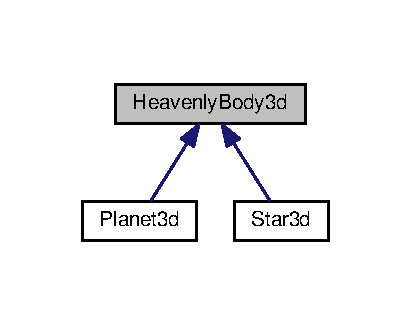
\includegraphics[width=197pt]{dc/dc8/classHeavenlyBody3d__inherit__graph}
\end{center}
\end{figure}


\-Collaboration diagram for \-Heavenly\-Body3d\-:
\nopagebreak
\begin{figure}[H]
\begin{center}
\leavevmode
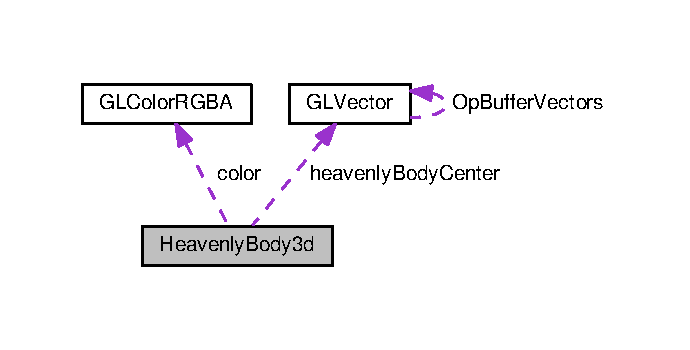
\includegraphics[width=331pt]{d0/d69/classHeavenlyBody3d__coll__graph}
\end{center}
\end{figure}
\subsection*{\-Public \-Member \-Functions}
\begin{DoxyCompactItemize}
\item 
\hyperlink{classHeavenlyBody3d_aa720873967d60dd36a7531545f25f5ce}{\-Heavenly\-Body3d} (\hyperlink{classHeavenlyBody}{\-Heavenly\-Body} $\ast$heavenly\-Body)
\begin{DoxyCompactList}\small\item\em \-Init the 3d objects. \end{DoxyCompactList}\item 
virtual void \hyperlink{classHeavenlyBody3d_a030592ed6fd43987d2b004f56a3ab3a8}{paint\-Heavenly\-Body3d} ()
\begin{DoxyCompactList}\small\item\em \-Paint the heavebly bodies. \end{DoxyCompactList}\item 
virtual void \hyperlink{classHeavenlyBody3d_ac1c46a03505f9b7bb57191f22d50ba27}{calculate\-Heavenly\-Body3d} ()
\begin{DoxyCompactList}\small\item\em \-Calculate the heavenly bodies. \end{DoxyCompactList}\item 
void \hyperlink{classHeavenlyBody3d_abc21e2ca9a6222ef3edfac68738ecb7d}{set\-Orbit\-Visisble} (bool orbit\-Visisble)
\begin{DoxyCompactList}\small\item\em \-Set or unset orbit visible. \end{DoxyCompactList}\item 
double \hyperlink{classHeavenlyBody3d_a6a626af4873c1783a7134a75aa27936b}{get\-Radius} ()
\begin{DoxyCompactList}\small\item\em \-Get the radius of the heavenly body 3d. \end{DoxyCompactList}\item 
\hyperlink{classGLVector}{\-G\-L\-Vector} \hyperlink{classHeavenlyBody3d_abc8856ee19131167a631f66cb0e40105}{get\-Center} ()
\begin{DoxyCompactList}\small\item\em get the center of the heavenly body 3d. \end{DoxyCompactList}\item 
\-Q\-String \hyperlink{classHeavenlyBody3d_afde15f252ebff5b5a791f42ad6aca61d}{get\-Name} ()
\begin{DoxyCompactList}\small\item\em \-Get the name of the heavenly body 3d. \end{DoxyCompactList}\item 
double \hyperlink{classHeavenlyBody3d_aa5abdb6a4b58366c48f86b41b3c24574}{calculate\-Distance} (\hyperlink{classHeavenlyBody3d}{\-Heavenly\-Body3d} $\ast$heavenly\-Body3d)
\begin{DoxyCompactList}\small\item\em \-Calculate the distance between the given heavenly body 3d and the current. \end{DoxyCompactList}\end{DoxyCompactItemize}
\subsection*{\-Protected \-Member \-Functions}
\begin{DoxyCompactItemize}
\item 
bool \hyperlink{classHeavenlyBody3d_a13a4439fcde475a19632b84e3e244446}{is\-Orbit\-Visisble} ()
\begin{DoxyCompactList}\small\item\em \-Get state of orbit visible. \end{DoxyCompactList}\end{DoxyCompactItemize}
\subsection*{\-Protected \-Attributes}
\begin{DoxyCompactItemize}
\item 
\hyperlink{classGLColorRGBA}{\-G\-L\-Color\-R\-G\-B\-A} \hyperlink{classHeavenlyBody3d_a2ebcfe6746f12921e1ef0c9bfeb4a9cb}{color}
\item 
float \hyperlink{classHeavenlyBody3d_a287510419f9dd9019fbfd56154c15f75}{x}
\item 
float \hyperlink{classHeavenlyBody3d_a219f2f76157b162a89a4bbdbec72dbff}{y}
\item 
\hyperlink{classGLVector}{\-G\-L\-Vector} \hyperlink{classHeavenlyBody3d_a3fa03680a708c4c58d4db74b8fdf58fb}{heavenly\-Body\-Center}
\end{DoxyCompactItemize}


\subsection{\-Detailed \-Description}
\-Class to calculate and paint the heavenly bodies.

\begin{DoxyAuthor}{\-Author}
\-Fabian \-Deitelhoff $<$\href{mailto:FH@FabianDeitelhoff.de}{\tt \-F\-H@\-Fabian\-Deitelhoff.\-de}$>$ 

\-Christof \-Geisler $<$\href{mailto:christof.geisler@stud.fh-swf.de}{\tt christof.\-geisler@stud.\-fh-\/swf.\-de}$>$ 
\end{DoxyAuthor}


\subsection{\-Constructor \& \-Destructor \-Documentation}
\hypertarget{classHeavenlyBody3d_aa720873967d60dd36a7531545f25f5ce}{
\index{\-Heavenly\-Body3d@{\-Heavenly\-Body3d}!\-Heavenly\-Body3d@{\-Heavenly\-Body3d}}
\index{\-Heavenly\-Body3d@{\-Heavenly\-Body3d}!HeavenlyBody3d@{\-Heavenly\-Body3d}}
\subsubsection[{\-Heavenly\-Body3d}]{\setlength{\rightskip}{0pt plus 5cm}\-Heavenly\-Body3d\-::\-Heavenly\-Body3d (
\begin{DoxyParamCaption}
\item[{{\bf \-Heavenly\-Body} $\ast$}]{heavenly\-Body}
\end{DoxyParamCaption}
)}}
\label{db/d73/classHeavenlyBody3d_aa720873967d60dd36a7531545f25f5ce}


\-Init the 3d objects. 


\begin{DoxyParams}{\-Parameters}
{\em heavenly\-Body} & \\
\hline
\end{DoxyParams}

\begin{DoxyCode}
{
    name = heavenlyBody->getName();

    color = GLColorRGBA(heavenlyBody->getColor().redF(),
                        heavenlyBody->getColor().greenF(),
                        heavenlyBody->getColor().blueF(),
                        heavenlyBody->getColor().alphaF());

    radius = GLdouble((heavenlyBody->getDiameter() / 2.0) / 3000.0);

    x = 0;
    y = 0;
}
\end{DoxyCode}


\subsection{\-Member \-Function \-Documentation}
\hypertarget{classHeavenlyBody3d_aa5abdb6a4b58366c48f86b41b3c24574}{
\index{\-Heavenly\-Body3d@{\-Heavenly\-Body3d}!calculate\-Distance@{calculate\-Distance}}
\index{calculate\-Distance@{calculate\-Distance}!HeavenlyBody3d@{\-Heavenly\-Body3d}}
\subsubsection[{calculate\-Distance}]{\setlength{\rightskip}{0pt plus 5cm}double \-Heavenly\-Body3d\-::calculate\-Distance (
\begin{DoxyParamCaption}
\item[{{\bf \-Heavenly\-Body3d} $\ast$}]{heavenly\-Body3d}
\end{DoxyParamCaption}
)}}
\label{db/d73/classHeavenlyBody3d_aa5abdb6a4b58366c48f86b41b3c24574}


\-Calculate the distance between the given heavenly body 3d and the current. 


\begin{DoxyParams}{\-Parameters}
{\em heavenly\-Body3d} & \\
\hline
\end{DoxyParams}
\begin{DoxyReturn}{\-Returns}
double 
\end{DoxyReturn}

\begin{DoxyCode}
{
    double x = pow(heavenlyBody3d->getCenter().x() - getCenter().x(), 2);
    double y = pow(heavenlyBody3d->getCenter().y() - getCenter().y(), 2);
    double z = pow(heavenlyBody3d->getCenter().z() - getCenter().z(), 2);

    return sqrt(x + y + z);
}
\end{DoxyCode}
\hypertarget{classHeavenlyBody3d_ac1c46a03505f9b7bb57191f22d50ba27}{
\index{\-Heavenly\-Body3d@{\-Heavenly\-Body3d}!calculate\-Heavenly\-Body3d@{calculate\-Heavenly\-Body3d}}
\index{calculate\-Heavenly\-Body3d@{calculate\-Heavenly\-Body3d}!HeavenlyBody3d@{\-Heavenly\-Body3d}}
\subsubsection[{calculate\-Heavenly\-Body3d}]{\setlength{\rightskip}{0pt plus 5cm}void \-Heavenly\-Body3d\-::calculate\-Heavenly\-Body3d (
\begin{DoxyParamCaption}
{}
\end{DoxyParamCaption}
)\hspace{0.3cm}{\ttfamily  \mbox{[}virtual\mbox{]}}}}
\label{db/d73/classHeavenlyBody3d_ac1c46a03505f9b7bb57191f22d50ba27}


\-Calculate the heavenly bodies. 



\-Reimplemented in \hyperlink{classPlanet3d_af486055f2af946f84c309c93096596fd}{\-Planet3d}.


\begin{DoxyCode}
{ }
\end{DoxyCode}
\hypertarget{classHeavenlyBody3d_abc8856ee19131167a631f66cb0e40105}{
\index{\-Heavenly\-Body3d@{\-Heavenly\-Body3d}!get\-Center@{get\-Center}}
\index{get\-Center@{get\-Center}!HeavenlyBody3d@{\-Heavenly\-Body3d}}
\subsubsection[{get\-Center}]{\setlength{\rightskip}{0pt plus 5cm}{\bf \-G\-L\-Vector} \-Heavenly\-Body3d\-::get\-Center (
\begin{DoxyParamCaption}
{}
\end{DoxyParamCaption}
)}}
\label{db/d73/classHeavenlyBody3d_abc8856ee19131167a631f66cb0e40105}


get the center of the heavenly body 3d. 

\begin{DoxyReturn}{\-Returns}
\hyperlink{classGLVector}{\-G\-L\-Vector} 
\end{DoxyReturn}

\begin{DoxyCode}
{
    return heavenlyBodyCenter;
}
\end{DoxyCode}
\hypertarget{classHeavenlyBody3d_afde15f252ebff5b5a791f42ad6aca61d}{
\index{\-Heavenly\-Body3d@{\-Heavenly\-Body3d}!get\-Name@{get\-Name}}
\index{get\-Name@{get\-Name}!HeavenlyBody3d@{\-Heavenly\-Body3d}}
\subsubsection[{get\-Name}]{\setlength{\rightskip}{0pt plus 5cm}\-Q\-String \-Heavenly\-Body3d\-::get\-Name (
\begin{DoxyParamCaption}
{}
\end{DoxyParamCaption}
)}}
\label{db/d73/classHeavenlyBody3d_afde15f252ebff5b5a791f42ad6aca61d}


\-Get the name of the heavenly body 3d. 

\begin{DoxyReturn}{\-Returns}
\-Q\-String 
\end{DoxyReturn}

\begin{DoxyCode}
{
    return name;
}
\end{DoxyCode}
\hypertarget{classHeavenlyBody3d_a6a626af4873c1783a7134a75aa27936b}{
\index{\-Heavenly\-Body3d@{\-Heavenly\-Body3d}!get\-Radius@{get\-Radius}}
\index{get\-Radius@{get\-Radius}!HeavenlyBody3d@{\-Heavenly\-Body3d}}
\subsubsection[{get\-Radius}]{\setlength{\rightskip}{0pt plus 5cm}double \-Heavenly\-Body3d\-::get\-Radius (
\begin{DoxyParamCaption}
{}
\end{DoxyParamCaption}
)}}
\label{db/d73/classHeavenlyBody3d_a6a626af4873c1783a7134a75aa27936b}


\-Get the radius of the heavenly body 3d. 

\begin{DoxyReturn}{\-Returns}
double 
\end{DoxyReturn}

\begin{DoxyCode}
{
    return radius;
}
\end{DoxyCode}
\hypertarget{classHeavenlyBody3d_a13a4439fcde475a19632b84e3e244446}{
\index{\-Heavenly\-Body3d@{\-Heavenly\-Body3d}!is\-Orbit\-Visisble@{is\-Orbit\-Visisble}}
\index{is\-Orbit\-Visisble@{is\-Orbit\-Visisble}!HeavenlyBody3d@{\-Heavenly\-Body3d}}
\subsubsection[{is\-Orbit\-Visisble}]{\setlength{\rightskip}{0pt plus 5cm}bool \-Heavenly\-Body3d\-::is\-Orbit\-Visisble (
\begin{DoxyParamCaption}
{}
\end{DoxyParamCaption}
)\hspace{0.3cm}{\ttfamily  \mbox{[}protected\mbox{]}}}}
\label{db/d73/classHeavenlyBody3d_a13a4439fcde475a19632b84e3e244446}


\-Get state of orbit visible. 

\begin{DoxyReturn}{\-Returns}
bool 
\end{DoxyReturn}

\begin{DoxyCode}
{
    return orbitVisisble;
}
\end{DoxyCode}
\hypertarget{classHeavenlyBody3d_a030592ed6fd43987d2b004f56a3ab3a8}{
\index{\-Heavenly\-Body3d@{\-Heavenly\-Body3d}!paint\-Heavenly\-Body3d@{paint\-Heavenly\-Body3d}}
\index{paint\-Heavenly\-Body3d@{paint\-Heavenly\-Body3d}!HeavenlyBody3d@{\-Heavenly\-Body3d}}
\subsubsection[{paint\-Heavenly\-Body3d}]{\setlength{\rightskip}{0pt plus 5cm}void \-Heavenly\-Body3d\-::paint\-Heavenly\-Body3d (
\begin{DoxyParamCaption}
{}
\end{DoxyParamCaption}
)\hspace{0.3cm}{\ttfamily  \mbox{[}virtual\mbox{]}}}}
\label{db/d73/classHeavenlyBody3d_a030592ed6fd43987d2b004f56a3ab3a8}


\-Paint the heavebly bodies. 



\-Reimplemented in \hyperlink{classPlanet3d_a2e504935919360a2015b50c103798dd8}{\-Planet3d}, and \hyperlink{classStar3d_a131a6612a83da74b25db2ff389e91424}{\-Star3d}.


\begin{DoxyCode}
{
    glMaterialfv(GL_FRONT, GL_AMBIENT_AND_DIFFUSE, color.fv());
    glMateriali(GL_FRONT, GL_SHININESS, 100);

    glutSolidSphere(radius, 32, 32);
}
\end{DoxyCode}
\hypertarget{classHeavenlyBody3d_abc21e2ca9a6222ef3edfac68738ecb7d}{
\index{\-Heavenly\-Body3d@{\-Heavenly\-Body3d}!set\-Orbit\-Visisble@{set\-Orbit\-Visisble}}
\index{set\-Orbit\-Visisble@{set\-Orbit\-Visisble}!HeavenlyBody3d@{\-Heavenly\-Body3d}}
\subsubsection[{set\-Orbit\-Visisble}]{\setlength{\rightskip}{0pt plus 5cm}void \-Heavenly\-Body3d\-::set\-Orbit\-Visisble (
\begin{DoxyParamCaption}
\item[{bool}]{orbit\-Visisble}
\end{DoxyParamCaption}
)}}
\label{db/d73/classHeavenlyBody3d_abc21e2ca9a6222ef3edfac68738ecb7d}


\-Set or unset orbit visible. 


\begin{DoxyParams}{\-Parameters}
{\em orbit\-Visisble} & \\
\hline
\end{DoxyParams}

\begin{DoxyCode}
{
    this->orbitVisisble = orbitVisisble;
}
\end{DoxyCode}


\subsection{\-Member \-Data \-Documentation}
\hypertarget{classHeavenlyBody3d_a2ebcfe6746f12921e1ef0c9bfeb4a9cb}{
\index{\-Heavenly\-Body3d@{\-Heavenly\-Body3d}!color@{color}}
\index{color@{color}!HeavenlyBody3d@{\-Heavenly\-Body3d}}
\subsubsection[{color}]{\setlength{\rightskip}{0pt plus 5cm}{\bf \-G\-L\-Color\-R\-G\-B\-A} {\bf \-Heavenly\-Body3d\-::color}\hspace{0.3cm}{\ttfamily  \mbox{[}protected\mbox{]}}}}
\label{db/d73/classHeavenlyBody3d_a2ebcfe6746f12921e1ef0c9bfeb4a9cb}
\hypertarget{classHeavenlyBody3d_a3fa03680a708c4c58d4db74b8fdf58fb}{
\index{\-Heavenly\-Body3d@{\-Heavenly\-Body3d}!heavenly\-Body\-Center@{heavenly\-Body\-Center}}
\index{heavenly\-Body\-Center@{heavenly\-Body\-Center}!HeavenlyBody3d@{\-Heavenly\-Body3d}}
\subsubsection[{heavenly\-Body\-Center}]{\setlength{\rightskip}{0pt plus 5cm}{\bf \-G\-L\-Vector} {\bf \-Heavenly\-Body3d\-::heavenly\-Body\-Center}\hspace{0.3cm}{\ttfamily  \mbox{[}protected\mbox{]}}}}
\label{db/d73/classHeavenlyBody3d_a3fa03680a708c4c58d4db74b8fdf58fb}
\hypertarget{classHeavenlyBody3d_a287510419f9dd9019fbfd56154c15f75}{
\index{\-Heavenly\-Body3d@{\-Heavenly\-Body3d}!x@{x}}
\index{x@{x}!HeavenlyBody3d@{\-Heavenly\-Body3d}}
\subsubsection[{x}]{\setlength{\rightskip}{0pt plus 5cm}float {\bf \-Heavenly\-Body3d\-::x}\hspace{0.3cm}{\ttfamily  \mbox{[}protected\mbox{]}}}}
\label{db/d73/classHeavenlyBody3d_a287510419f9dd9019fbfd56154c15f75}
\hypertarget{classHeavenlyBody3d_a219f2f76157b162a89a4bbdbec72dbff}{
\index{\-Heavenly\-Body3d@{\-Heavenly\-Body3d}!y@{y}}
\index{y@{y}!HeavenlyBody3d@{\-Heavenly\-Body3d}}
\subsubsection[{y}]{\setlength{\rightskip}{0pt plus 5cm}float {\bf \-Heavenly\-Body3d\-::y}\hspace{0.3cm}{\ttfamily  \mbox{[}protected\mbox{]}}}}
\label{db/d73/classHeavenlyBody3d_a219f2f76157b162a89a4bbdbec72dbff}


\-The documentation for this class was generated from the following files\-:\begin{DoxyCompactItemize}
\item 
visualization/heavenlybody/\hyperlink{heavenlybody3d_8h}{heavenlybody3d.\-h}\item 
visualization/heavenlybody/\hyperlink{heavenlybody3d_8cpp}{heavenlybody3d.\-cpp}\end{DoxyCompactItemize}

\hypertarget{classHeavenlyBodyComboBoxModel}{
\section{\-Heavenly\-Body\-Combo\-Box\-Model \-Class \-Reference}
\label{dd/d88/classHeavenlyBodyComboBoxModel}\index{\-Heavenly\-Body\-Combo\-Box\-Model@{\-Heavenly\-Body\-Combo\-Box\-Model}}
}


{\ttfamily \#include $<$heavenlybodycomboboxmodel.\-h$>$}

\subsection*{\-Public \-Member \-Functions}
\begin{DoxyCompactItemize}
\item 
\hyperlink{classHeavenlyBodyComboBoxModel_af1f95ee9f2c7f9bd134e5111e21528b4}{\-Heavenly\-Body\-Combo\-Box\-Model} ()
\begin{DoxyCompactList}\small\item\em \-Default constructor for the heavenly body combo box, inherit from \-Q\-Abstract\-Item\-Model. \end{DoxyCompactList}\item 
\-Q\-Model\-Index \hyperlink{classHeavenlyBodyComboBoxModel_aeb459de382f97296ffd4739a95bfd3eb}{index} (int row, int column, const \-Q\-Model\-Index \&parent=\-Q\-Model\-Index()) const 
\begin{DoxyCompactList}\small\item\em \-Create index and return it when possible. \end{DoxyCompactList}\item 
\-Q\-Model\-Index \hyperlink{classHeavenlyBodyComboBoxModel_a8dc114dec8426c6e6264302470dab392}{parent} (const \-Q\-Model\-Index \&index) const 
\begin{DoxyCompactList}\small\item\em \-Get complete \-Q\-Model\-Index for index. \end{DoxyCompactList}\item 
int \hyperlink{classHeavenlyBodyComboBoxModel_af9e833868b66e60566d27233529cc5ab}{row\-Count} (const \-Q\-Model\-Index \&index=\-Q\-Model\-Index()) const 
\begin{DoxyCompactList}\small\item\em \-Get the row count of index. \end{DoxyCompactList}\item 
int \hyperlink{classHeavenlyBodyComboBoxModel_a5cf2c26b6129647b144880b1472b4436}{column\-Count} (const \-Q\-Model\-Index \&index=\-Q\-Model\-Index()) const 
\begin{DoxyCompactList}\small\item\em \-Column count is always 1 for index. \end{DoxyCompactList}\item 
\-Q\-Variant \hyperlink{classHeavenlyBodyComboBoxModel_ab32452909de0e4238d357fe183759583}{data} (const \-Q\-Model\-Index \&index, int role=\-Qt\-::\-Display\-Role) const 
\begin{DoxyCompactList}\small\item\em \-Get the name of the heavenly body at the marked row. \end{DoxyCompactList}\item 
void \hyperlink{classHeavenlyBodyComboBoxModel_a7d7afd44d28fc5fb9d7c99a2295f81e7}{set\-Data} (\-Q\-List$<$ \hyperlink{classHeavenlyBody}{\-Heavenly\-Body} $\ast$ $>$ entities)
\begin{DoxyCompactList}\small\item\em \-Set entities to combo box. \end{DoxyCompactList}\item 
\hyperlink{classHeavenlyBody}{\-Heavenly\-Body} $\ast$ \hyperlink{classHeavenlyBodyComboBoxModel_a5ab4dae7941519612bcbcc7e1b6463eb}{get\-Heavenly\-Body} (int index)
\begin{DoxyCompactList}\small\item\em \-Getter for heavenly body. \end{DoxyCompactList}\item 
int \hyperlink{classHeavenlyBodyComboBoxModel_ac57200d9257538babfdb200a0a661dd3}{get\-Heavenly\-Body\-Index} (\hyperlink{classHeavenlyBody}{\-Heavenly\-Body} $\ast$heavenly\-Body)
\begin{DoxyCompactList}\small\item\em \-Get the index of the given heavenly body. \end{DoxyCompactList}\end{DoxyCompactItemize}


\subsection{\-Detailed \-Description}
\-Class for the model of heavenly body combo box.

\begin{DoxyAuthor}{\-Author}
\-Fabian \-Deitelhoff $<$\href{mailto:FH@FabianDeitelhoff.de}{\tt \-F\-H@\-Fabian\-Deitelhoff.\-de}$>$ 

\-Christof \-Geisler $<$\href{mailto:christof.geisler@stud.fh-swf.de}{\tt christof.\-geisler@stud.\-fh-\/swf.\-de}$>$ 
\end{DoxyAuthor}


\subsection{\-Constructor \& \-Destructor \-Documentation}
\hypertarget{classHeavenlyBodyComboBoxModel_af1f95ee9f2c7f9bd134e5111e21528b4}{
\index{\-Heavenly\-Body\-Combo\-Box\-Model@{\-Heavenly\-Body\-Combo\-Box\-Model}!\-Heavenly\-Body\-Combo\-Box\-Model@{\-Heavenly\-Body\-Combo\-Box\-Model}}
\index{\-Heavenly\-Body\-Combo\-Box\-Model@{\-Heavenly\-Body\-Combo\-Box\-Model}!HeavenlyBodyComboBoxModel@{\-Heavenly\-Body\-Combo\-Box\-Model}}
\subsubsection[{\-Heavenly\-Body\-Combo\-Box\-Model}]{\setlength{\rightskip}{0pt plus 5cm}\-Heavenly\-Body\-Combo\-Box\-Model\-::\-Heavenly\-Body\-Combo\-Box\-Model (
\begin{DoxyParamCaption}
{}
\end{DoxyParamCaption}
)}}
\label{dd/d88/classHeavenlyBodyComboBoxModel_af1f95ee9f2c7f9bd134e5111e21528b4}


\-Default constructor for the heavenly body combo box, inherit from \-Q\-Abstract\-Item\-Model. 


\begin{DoxyCode}
    : QAbstractItemModel()
{
}
\end{DoxyCode}


\subsection{\-Member \-Function \-Documentation}
\hypertarget{classHeavenlyBodyComboBoxModel_a5cf2c26b6129647b144880b1472b4436}{
\index{\-Heavenly\-Body\-Combo\-Box\-Model@{\-Heavenly\-Body\-Combo\-Box\-Model}!column\-Count@{column\-Count}}
\index{column\-Count@{column\-Count}!HeavenlyBodyComboBoxModel@{\-Heavenly\-Body\-Combo\-Box\-Model}}
\subsubsection[{column\-Count}]{\setlength{\rightskip}{0pt plus 5cm}int \-Heavenly\-Body\-Combo\-Box\-Model\-::column\-Count (
\begin{DoxyParamCaption}
\item[{const \-Q\-Model\-Index \&}]{index = {\ttfamily \-Q\-Model\-Index()}}
\end{DoxyParamCaption}
) const}}
\label{dd/d88/classHeavenlyBodyComboBoxModel_a5cf2c26b6129647b144880b1472b4436}


\-Column count is always 1 for index. 


\begin{DoxyParams}{\-Parameters}
{\em index} & \\
\hline
\end{DoxyParams}
\begin{DoxyReturn}{\-Returns}
int 
\end{DoxyReturn}

\begin{DoxyCode}
{
    return 1;
}
\end{DoxyCode}
\hypertarget{classHeavenlyBodyComboBoxModel_ab32452909de0e4238d357fe183759583}{
\index{\-Heavenly\-Body\-Combo\-Box\-Model@{\-Heavenly\-Body\-Combo\-Box\-Model}!data@{data}}
\index{data@{data}!HeavenlyBodyComboBoxModel@{\-Heavenly\-Body\-Combo\-Box\-Model}}
\subsubsection[{data}]{\setlength{\rightskip}{0pt plus 5cm}\-Q\-Variant \-Heavenly\-Body\-Combo\-Box\-Model\-::data (
\begin{DoxyParamCaption}
\item[{const \-Q\-Model\-Index \&}]{index, }
\item[{int}]{role = {\ttfamily \-Qt\-:\-:\-Display\-Role}}
\end{DoxyParamCaption}
) const}}
\label{dd/d88/classHeavenlyBodyComboBoxModel_ab32452909de0e4238d357fe183759583}


\-Get the name of the heavenly body at the marked row. 


\begin{DoxyParams}{\-Parameters}
{\em index} & \\
\hline
{\em role} & \\
\hline
\end{DoxyParams}
\begin{DoxyReturn}{\-Returns}
\-Q\-Variant 
\end{DoxyReturn}

\begin{DoxyCode}
{
    if (!index.isValid() || role != Qt::DisplayRole)
    {
        return QVariant();
    }

    return entities.at(index.row())->getName();
}
\end{DoxyCode}
\hypertarget{classHeavenlyBodyComboBoxModel_a5ab4dae7941519612bcbcc7e1b6463eb}{
\index{\-Heavenly\-Body\-Combo\-Box\-Model@{\-Heavenly\-Body\-Combo\-Box\-Model}!get\-Heavenly\-Body@{get\-Heavenly\-Body}}
\index{get\-Heavenly\-Body@{get\-Heavenly\-Body}!HeavenlyBodyComboBoxModel@{\-Heavenly\-Body\-Combo\-Box\-Model}}
\subsubsection[{get\-Heavenly\-Body}]{\setlength{\rightskip}{0pt plus 5cm}{\bf \-Heavenly\-Body} $\ast$ \-Heavenly\-Body\-Combo\-Box\-Model\-::get\-Heavenly\-Body (
\begin{DoxyParamCaption}
\item[{int}]{index}
\end{DoxyParamCaption}
)}}
\label{dd/d88/classHeavenlyBodyComboBoxModel_a5ab4dae7941519612bcbcc7e1b6463eb}


\-Getter for heavenly body. 


\begin{DoxyParams}{\-Parameters}
{\em index} & \\
\hline
\end{DoxyParams}
\begin{DoxyReturn}{\-Returns}
\hyperlink{classHeavenlyBody}{\-Heavenly\-Body} $\ast$ 
\end{DoxyReturn}

\begin{DoxyCode}
{
    if (index < 0 || index >= entities.size())
    {
        return 0;
    }

    return entities.at(index);
}
\end{DoxyCode}
\hypertarget{classHeavenlyBodyComboBoxModel_ac57200d9257538babfdb200a0a661dd3}{
\index{\-Heavenly\-Body\-Combo\-Box\-Model@{\-Heavenly\-Body\-Combo\-Box\-Model}!get\-Heavenly\-Body\-Index@{get\-Heavenly\-Body\-Index}}
\index{get\-Heavenly\-Body\-Index@{get\-Heavenly\-Body\-Index}!HeavenlyBodyComboBoxModel@{\-Heavenly\-Body\-Combo\-Box\-Model}}
\subsubsection[{get\-Heavenly\-Body\-Index}]{\setlength{\rightskip}{0pt plus 5cm}int \-Heavenly\-Body\-Combo\-Box\-Model\-::get\-Heavenly\-Body\-Index (
\begin{DoxyParamCaption}
\item[{{\bf \-Heavenly\-Body} $\ast$}]{heavenly\-Body}
\end{DoxyParamCaption}
)}}
\label{dd/d88/classHeavenlyBodyComboBoxModel_ac57200d9257538babfdb200a0a661dd3}


\-Get the index of the given heavenly body. 


\begin{DoxyParams}{\-Parameters}
{\em heavenly\-Body} & \\
\hline
\end{DoxyParams}
\begin{DoxyReturn}{\-Returns}
int 
\end{DoxyReturn}

\begin{DoxyCode}
{
    if (!heavenlyBody)
    {
        return -1;
    }

    int row = -1;
    foreach(HeavenlyBody *entity, entities)
    {
        row++;
        if ((*entity) == (*heavenlyBody))
        {
            break;
        }
    }

    return row;
}
\end{DoxyCode}
\hypertarget{classHeavenlyBodyComboBoxModel_aeb459de382f97296ffd4739a95bfd3eb}{
\index{\-Heavenly\-Body\-Combo\-Box\-Model@{\-Heavenly\-Body\-Combo\-Box\-Model}!index@{index}}
\index{index@{index}!HeavenlyBodyComboBoxModel@{\-Heavenly\-Body\-Combo\-Box\-Model}}
\subsubsection[{index}]{\setlength{\rightskip}{0pt plus 5cm}\-Q\-Model\-Index \-Heavenly\-Body\-Combo\-Box\-Model\-::index (
\begin{DoxyParamCaption}
\item[{int}]{row, }
\item[{int}]{column, }
\item[{const \-Q\-Model\-Index \&}]{parent = {\ttfamily \-Q\-Model\-Index()}}
\end{DoxyParamCaption}
) const}}
\label{dd/d88/classHeavenlyBodyComboBoxModel_aeb459de382f97296ffd4739a95bfd3eb}


\-Create index and return it when possible. 


\begin{DoxyParams}{\-Parameters}
{\em row} & \\
\hline
{\em column} & \\
\hline
{\em parent} & \\
\hline
\end{DoxyParams}
\begin{DoxyReturn}{\-Returns}
\-Q\-Model\-Index 
\end{DoxyReturn}

\begin{DoxyCode}
{
    if ( column < 0 || row < 0 )
    {
        return QModelIndex();
    }

    return createIndex(row, column); //, entities.at(row));
}
\end{DoxyCode}
\hypertarget{classHeavenlyBodyComboBoxModel_a8dc114dec8426c6e6264302470dab392}{
\index{\-Heavenly\-Body\-Combo\-Box\-Model@{\-Heavenly\-Body\-Combo\-Box\-Model}!parent@{parent}}
\index{parent@{parent}!HeavenlyBodyComboBoxModel@{\-Heavenly\-Body\-Combo\-Box\-Model}}
\subsubsection[{parent}]{\setlength{\rightskip}{0pt plus 5cm}\-Q\-Model\-Index \-Heavenly\-Body\-Combo\-Box\-Model\-::parent (
\begin{DoxyParamCaption}
\item[{const \-Q\-Model\-Index \&}]{index}
\end{DoxyParamCaption}
) const}}
\label{dd/d88/classHeavenlyBodyComboBoxModel_a8dc114dec8426c6e6264302470dab392}


\-Get complete \-Q\-Model\-Index for index. 


\begin{DoxyParams}{\-Parameters}
{\em index} & \\
\hline
\end{DoxyParams}
\begin{DoxyReturn}{\-Returns}
\-Q\-Model\-Index 
\end{DoxyReturn}

\begin{DoxyCode}
{
    return QModelIndex();
}
\end{DoxyCode}
\hypertarget{classHeavenlyBodyComboBoxModel_af9e833868b66e60566d27233529cc5ab}{
\index{\-Heavenly\-Body\-Combo\-Box\-Model@{\-Heavenly\-Body\-Combo\-Box\-Model}!row\-Count@{row\-Count}}
\index{row\-Count@{row\-Count}!HeavenlyBodyComboBoxModel@{\-Heavenly\-Body\-Combo\-Box\-Model}}
\subsubsection[{row\-Count}]{\setlength{\rightskip}{0pt plus 5cm}int \-Heavenly\-Body\-Combo\-Box\-Model\-::row\-Count (
\begin{DoxyParamCaption}
\item[{const \-Q\-Model\-Index \&}]{index = {\ttfamily \-Q\-Model\-Index()}}
\end{DoxyParamCaption}
) const}}
\label{dd/d88/classHeavenlyBodyComboBoxModel_af9e833868b66e60566d27233529cc5ab}


\-Get the row count of index. 


\begin{DoxyParams}{\-Parameters}
{\em index} & \\
\hline
\end{DoxyParams}
\begin{DoxyReturn}{\-Returns}
int 
\end{DoxyReturn}

\begin{DoxyCode}
{
    return entities.size();
}
\end{DoxyCode}
\hypertarget{classHeavenlyBodyComboBoxModel_a7d7afd44d28fc5fb9d7c99a2295f81e7}{
\index{\-Heavenly\-Body\-Combo\-Box\-Model@{\-Heavenly\-Body\-Combo\-Box\-Model}!set\-Data@{set\-Data}}
\index{set\-Data@{set\-Data}!HeavenlyBodyComboBoxModel@{\-Heavenly\-Body\-Combo\-Box\-Model}}
\subsubsection[{set\-Data}]{\setlength{\rightskip}{0pt plus 5cm}void \-Heavenly\-Body\-Combo\-Box\-Model\-::set\-Data (
\begin{DoxyParamCaption}
\item[{\-Q\-List$<$ {\bf \-Heavenly\-Body} $\ast$ $>$}]{entities}
\end{DoxyParamCaption}
)}}
\label{dd/d88/classHeavenlyBodyComboBoxModel_a7d7afd44d28fc5fb9d7c99a2295f81e7}


\-Set entities to combo box. 


\begin{DoxyParams}{\-Parameters}
{\em entities} & \\
\hline
\end{DoxyParams}

\begin{DoxyCode}
{
    this->entities.clear();
    this->entities.append(entities);

    reset();
}
\end{DoxyCode}


\-The documentation for this class was generated from the following files\-:\begin{DoxyCompactItemize}
\item 
model/heavenlybody/\hyperlink{heavenlybodycomboboxmodel_8h}{heavenlybodycomboboxmodel.\-h}\item 
model/heavenlybody/\hyperlink{heavenlybodycomboboxmodel_8cpp}{heavenlybodycomboboxmodel.\-cpp}\end{DoxyCompactItemize}

\hypertarget{classHeavenlyBodyDetails}{
\section{\-Heavenly\-Body\-Details \-Class \-Reference}
\label{dd/d37/classHeavenlyBodyDetails}\index{\-Heavenly\-Body\-Details@{\-Heavenly\-Body\-Details}}
}


{\ttfamily \#include $<$heavenlybodydetails.\-h$>$}

\subsection*{\-Public \-Member \-Functions}
\begin{DoxyCompactItemize}
\item 
\hyperlink{classHeavenlyBodyDetails_a054ec45af11e8f42cba7f0b40eb5f8e8}{\-Heavenly\-Body\-Details} (\-Q\-Widget $\ast$parent=0, \hyperlink{classHeavenlyBodyModel}{\-Heavenly\-Body\-Model} $\ast$heavenly\-Body\-Model=0, bool edit=false)
\begin{DoxyCompactList}\small\item\em \-Open dialog window to add or edit a heavenly body. \end{DoxyCompactList}\item 
\hyperlink{classHeavenlyBodyDetails_a7f2566a1ba36b51157a6d0c753a0c545}{$\sim$\-Heavenly\-Body\-Details} ()
\begin{DoxyCompactList}\small\item\em \-Destructor to close dialog. \end{DoxyCompactList}\end{DoxyCompactItemize}


\subsection{\-Detailed \-Description}
\-Class for the components to show the window heavenly body details.

\begin{DoxyAuthor}{\-Author}
\-Fabian \-Deitelhoff $<$\href{mailto:FH@FabianDeitelhoff.de}{\tt \-F\-H@\-Fabian\-Deitelhoff.\-de}$>$ 

\-Christof \-Geisler $<$\href{mailto:christof.geisler@stud.fh-swf.de}{\tt christof.\-geisler@stud.\-fh-\/swf.\-de}$>$ 
\end{DoxyAuthor}


\subsection{\-Constructor \& \-Destructor \-Documentation}
\hypertarget{classHeavenlyBodyDetails_a054ec45af11e8f42cba7f0b40eb5f8e8}{
\index{\-Heavenly\-Body\-Details@{\-Heavenly\-Body\-Details}!\-Heavenly\-Body\-Details@{\-Heavenly\-Body\-Details}}
\index{\-Heavenly\-Body\-Details@{\-Heavenly\-Body\-Details}!HeavenlyBodyDetails@{\-Heavenly\-Body\-Details}}
\subsubsection[{\-Heavenly\-Body\-Details}]{\setlength{\rightskip}{0pt plus 5cm}\-Heavenly\-Body\-Details\-::\-Heavenly\-Body\-Details (
\begin{DoxyParamCaption}
\item[{\-Q\-Widget $\ast$}]{parent = {\ttfamily 0}, }
\item[{{\bf \-Heavenly\-Body\-Model} $\ast$}]{heavenly\-Body\-Model = {\ttfamily 0}, }
\item[{bool}]{is\-Edit = {\ttfamily false}}
\end{DoxyParamCaption}
)}}
\label{dd/d37/classHeavenlyBodyDetails_a054ec45af11e8f42cba7f0b40eb5f8e8}


\-Open dialog window to add or edit a heavenly body. 


\begin{DoxyParams}{\-Parameters}
{\em parent} & \-Parent of this dialog. \\
\hline
{\em heavenly\-Body\-Model} & \-Model of the heavenly body table. \\
\hline
{\em is\-Edit} & \-If \-T\-R\-U\-E edit, else add heavenlybody. \\
\hline
\end{DoxyParams}

\begin{DoxyCode}
                                                                               
                                  :
    QDialog(parent),
    ui(new Ui::HeavenlyBodyDetails)
{
    ui->setupUi(this);

    setWindowFlags(windowFlags() ^ Qt::WindowContextHelpButtonHint);

    this->isEdit = isEdit;

    this->heavenlyBodyModel = heavenlyBodyModel;

    tmpColor = Qt::green;

    colorDialog = new QColorDialog(this);

    if (isEdit)
    {
        currentEntity = heavenlyBodyModel->getSelectedEntity();

        setWindowTitle(QString("Edit Heavenly Body '%1'").arg(currentEntity->
      getName()));

        ui->name->setText(currentEntity->getName());
        ui->diameter->setText(QString::number(currentEntity->getDiameter()));

        tmpColor = currentEntity->getColor();

        if (currentEntity->getType() == "S")
        {
            ui->star->setChecked(true);
        }
    }

    // Maybe StyleSheets are a better solution here?
    QPalette palette = ui->colorLabel->palette();
    palette.setColor(ui->colorLabel->backgroundRole(), tmpColor);
    ui->colorLabel->setPalette(palette);
}
\end{DoxyCode}
\hypertarget{classHeavenlyBodyDetails_a7f2566a1ba36b51157a6d0c753a0c545}{
\index{\-Heavenly\-Body\-Details@{\-Heavenly\-Body\-Details}!$\sim$\-Heavenly\-Body\-Details@{$\sim$\-Heavenly\-Body\-Details}}
\index{$\sim$\-Heavenly\-Body\-Details@{$\sim$\-Heavenly\-Body\-Details}!HeavenlyBodyDetails@{\-Heavenly\-Body\-Details}}
\subsubsection[{$\sim$\-Heavenly\-Body\-Details}]{\setlength{\rightskip}{0pt plus 5cm}\-Heavenly\-Body\-Details\-::$\sim$\-Heavenly\-Body\-Details (
\begin{DoxyParamCaption}
{}
\end{DoxyParamCaption}
)}}
\label{dd/d37/classHeavenlyBodyDetails_a7f2566a1ba36b51157a6d0c753a0c545}


\-Destructor to close dialog. 


\begin{DoxyCode}
{
    delete ui;
}
\end{DoxyCode}


\-The documentation for this class was generated from the following files\-:\begin{DoxyCompactItemize}
\item 
forms/heavenlybody/\hyperlink{heavenlybodydetails_8h}{heavenlybodydetails.\-h}\item 
forms/heavenlybody/\hyperlink{heavenlybodydetails_8cpp}{heavenlybodydetails.\-cpp}\end{DoxyCompactItemize}

\hypertarget{classHeavenlyBodyItemDelegate}{
\section{\-Heavenly\-Body\-Item\-Delegate \-Class \-Reference}
\label{dc/dc9/classHeavenlyBodyItemDelegate}\index{\-Heavenly\-Body\-Item\-Delegate@{\-Heavenly\-Body\-Item\-Delegate}}
}


{\ttfamily \#include $<$heavenlybodyitemdelegate.\-h$>$}

\subsection*{\-Public \-Member \-Functions}
\begin{DoxyCompactItemize}
\item 
\hyperlink{classHeavenlyBodyItemDelegate_ab16dfebe2c70f5b6468a65571546b9a9}{\-Heavenly\-Body\-Item\-Delegate} (\hyperlink{classHeavenlyBodyModel}{\-Heavenly\-Body\-Model} $\ast$heavenly\-Body\-Model)
\begin{DoxyCompactList}\small\item\em \-Set an other color to collumn 3 (color) when row is selected. \end{DoxyCompactList}\item 
void \hyperlink{classHeavenlyBodyItemDelegate_a79a286b97de08c04af5b65f5139db7d4}{paint} (\-Q\-Painter $\ast$painter, const \-Q\-Style\-Option\-View\-Item \&option, const \-Q\-Model\-Index \&index) const 
\begin{DoxyCompactList}\small\item\em \-Set the color of the selected color-\/collumn to the color of the heavenly body. \-Others to default. \end{DoxyCompactList}\end{DoxyCompactItemize}


\subsection{\-Detailed \-Description}
\-Class to enable an other color view in selected rows.

\begin{DoxyAuthor}{\-Author}
\-Fabian \-Deitelhoff $<$\href{mailto:FH@FabianDeitelhoff.de}{\tt \-F\-H@\-Fabian\-Deitelhoff.\-de}$>$ 

\-Christof \-Geisler $<$\href{mailto:christof.geisler@stud.fh-swf.de}{\tt christof.\-geisler@stud.\-fh-\/swf.\-de}$>$ 
\end{DoxyAuthor}


\subsection{\-Constructor \& \-Destructor \-Documentation}
\hypertarget{classHeavenlyBodyItemDelegate_ab16dfebe2c70f5b6468a65571546b9a9}{
\index{\-Heavenly\-Body\-Item\-Delegate@{\-Heavenly\-Body\-Item\-Delegate}!\-Heavenly\-Body\-Item\-Delegate@{\-Heavenly\-Body\-Item\-Delegate}}
\index{\-Heavenly\-Body\-Item\-Delegate@{\-Heavenly\-Body\-Item\-Delegate}!HeavenlyBodyItemDelegate@{\-Heavenly\-Body\-Item\-Delegate}}
\subsubsection[{\-Heavenly\-Body\-Item\-Delegate}]{\setlength{\rightskip}{0pt plus 5cm}\-Heavenly\-Body\-Item\-Delegate\-::\-Heavenly\-Body\-Item\-Delegate (
\begin{DoxyParamCaption}
\item[{{\bf \-Heavenly\-Body\-Model} $\ast$}]{heavenly\-Body\-Model}
\end{DoxyParamCaption}
)}}
\label{dc/dc9/classHeavenlyBodyItemDelegate_ab16dfebe2c70f5b6468a65571546b9a9}


\-Set an other color to collumn 3 (color) when row is selected. 


\begin{DoxyParams}{\-Parameters}
{\em heavenly\-Body\-Model} & \\
\hline
\end{DoxyParams}

\begin{DoxyCode}
{
    this->heavenlyBodyModel = heavenlyBodyModel;
}
\end{DoxyCode}


\subsection{\-Member \-Function \-Documentation}
\hypertarget{classHeavenlyBodyItemDelegate_a79a286b97de08c04af5b65f5139db7d4}{
\index{\-Heavenly\-Body\-Item\-Delegate@{\-Heavenly\-Body\-Item\-Delegate}!paint@{paint}}
\index{paint@{paint}!HeavenlyBodyItemDelegate@{\-Heavenly\-Body\-Item\-Delegate}}
\subsubsection[{paint}]{\setlength{\rightskip}{0pt plus 5cm}void \-Heavenly\-Body\-Item\-Delegate\-::paint (
\begin{DoxyParamCaption}
\item[{\-Q\-Painter $\ast$}]{painter, }
\item[{const \-Q\-Style\-Option\-View\-Item \&}]{option, }
\item[{const \-Q\-Model\-Index \&}]{index}
\end{DoxyParamCaption}
) const}}
\label{dc/dc9/classHeavenlyBodyItemDelegate_a79a286b97de08c04af5b65f5139db7d4}


\-Set the color of the selected color-\/collumn to the color of the heavenly body. \-Others to default. 


\begin{DoxyParams}{\-Parameters}
{\em painter} & \-Paint options \\
\hline
{\em option} & \-Style options. \\
\hline
{\em index} & \-Selected row. \\
\hline
\end{DoxyParams}

\begin{DoxyCode}
{
    if (index.column() == 3)
    {
        HeavenlyBody *heavenlyBody = heavenlyBodyModel->
      getHeavenlyBodyTableModel()->getHeavenlyBody(index.row());

        if (heavenlyBody)
        {
            painter->fillRect(option.rect, heavenlyBody->getColor());
        }
    }
    else
    {
        QItemDelegate::paint(painter, option, index);
    }
}
\end{DoxyCode}


\-The documentation for this class was generated from the following files\-:\begin{DoxyCompactItemize}
\item 
forms/heavenlybody/\hyperlink{heavenlybodyitemdelegate_8h}{heavenlybodyitemdelegate.\-h}\item 
forms/heavenlybody/\hyperlink{heavenlybodyitemdelegate_8cpp}{heavenlybodyitemdelegate.\-cpp}\end{DoxyCompactItemize}

\section{\-Heavenly\-Body\-Model \-Class \-Reference}
\label{d5/dae/classHeavenlyBodyModel}\index{\-Heavenly\-Body\-Model@{\-Heavenly\-Body\-Model}}
\subsection*{\-Public \-Member \-Functions}
\begin{DoxyCompactItemize}
\item 
void {\bfseries load\-All\-Heavenly\-Body\-Entities} ()\label{d5/dae/classHeavenlyBodyModel_a6930a1f2cabc1b5c715faeefa255b9b6}

\item 
{\bf \-Heavenly\-Body\-Table\-Model} $\ast$ {\bfseries get\-Heavenly\-Body\-Table\-Model} ()\label{d5/dae/classHeavenlyBodyModel_a8237cf4cab0e6b3b154ba7e4f70f9d56}

\item 
void {\bfseries set\-Selection\-Model} (\-Q\-Item\-Selection\-Model $\ast$selection\-Model)\label{d5/dae/classHeavenlyBodyModel_a13d3799b8e3ee537fdebe61a419160a9}

\item 
{\bf \-Heavenly\-Body} $\ast$ {\bfseries get\-Selected\-Entity} ()\label{d5/dae/classHeavenlyBodyModel_abc32e9a6e31b96a93d4dcd31e736be17}

\item 
bool {\bfseries is\-Entity\-Selected} ()\label{d5/dae/classHeavenlyBodyModel_aebbc9b5febaa4e709e6f2c433f7f99f5}

\item 
void {\bfseries add\-Entity} (\-Q\-String name, int diameter, \-Q\-Color color, \-Q\-String type)\label{d5/dae/classHeavenlyBodyModel_a181897be2a2724104384115dcf625457}

\item 
void {\bfseries update\-Entity} (\-Q\-String name, int diameter, \-Q\-Color color, \-Q\-String type)\label{d5/dae/classHeavenlyBodyModel_ad37a9019aa8a0f21a94b07d10b81e50b}

\item 
void {\bfseries delete\-Entity} ()\label{d5/dae/classHeavenlyBodyModel_a5d9f5cfdc3a128959ec9bd88ace1226f}

\end{DoxyCompactItemize}


\-The documentation for this class was generated from the following files\-:\begin{DoxyCompactItemize}
\item 
model/heavenlybody/heavenlybodymodel.\-h\item 
model/heavenlybody/heavenlybodymodel.\-cpp\end{DoxyCompactItemize}

\hypertarget{classHeavenlyBodyOverview}{
\section{\-Heavenly\-Body\-Overview \-Class \-Reference}
\label{d9/d59/classHeavenlyBodyOverview}\index{\-Heavenly\-Body\-Overview@{\-Heavenly\-Body\-Overview}}
}


{\ttfamily \#include $<$heavenlybodyoverview.\-h$>$}

\subsection*{\-Public \-Slots}
\begin{DoxyCompactItemize}
\item 
void \hyperlink{classHeavenlyBodyOverview_ad23b61bfb27f1b479eb965c84af55462}{on\-\_\-add\-\_\-clicked} ()
\begin{DoxyCompactList}\small\item\em \-Add a new heavenly body to the model. \end{DoxyCompactList}\item 
void \hyperlink{classHeavenlyBodyOverview_a1bf8ee9ed5de9b020979f2cffde51e97}{on\-\_\-edit\-\_\-clicked} ()
\begin{DoxyCompactList}\small\item\em \-Edit the selected heavenly body from the \-List. \end{DoxyCompactList}\item 
void \hyperlink{classHeavenlyBodyOverview_a280498f7189f4c6578803120028c3fb7}{on\-\_\-delete\-Entity\-\_\-clicked} ()
\begin{DoxyCompactList}\small\item\em \-Delete the selected heavenly body. \end{DoxyCompactList}\item 
void \hyperlink{classHeavenlyBodyOverview_a85de3eefb0dab6d69a3d82ac47437eb6}{double\-Clicked} (\-Q\-Model\-Index model\-Index)
\begin{DoxyCompactList}\small\item\em \-Enable double click to select a heavenly body. \end{DoxyCompactList}\end{DoxyCompactItemize}
\subsection*{\-Public \-Member \-Functions}
\begin{DoxyCompactItemize}
\item 
\hyperlink{classHeavenlyBodyOverview_a075b5a989998634fea2b7f5eab20f6d7}{\-Heavenly\-Body\-Overview} (\-Q\-Widget $\ast$parent=0, \hyperlink{classHeavenlyBodyModel}{\-Heavenly\-Body\-Model} $\ast$heavenly\-Body\-Model=0)
\begin{DoxyCompactList}\small\item\em \-Open the window of the heanenly body overview. \end{DoxyCompactList}\item 
\hyperlink{classHeavenlyBodyOverview_a170a2a848938c2b5b66dd1003b4fd5f2}{$\sim$\-Heavenly\-Body\-Overview} ()
\begin{DoxyCompactList}\small\item\em \-Delete the heavenly body overview window. \end{DoxyCompactList}\end{DoxyCompactItemize}


\subsection{\-Detailed \-Description}
\-Class with components to show the window heavenly body overview.

\begin{DoxyAuthor}{\-Author}
\-Fabian \-Deitelhoff $<$\href{mailto:FH@FabianDeitelhoff.de}{\tt \-F\-H@\-Fabian\-Deitelhoff.\-de}$>$ 

\-Christof \-Geisler $<$\href{mailto:christof.geisler@stud.fh-swf.de}{\tt christof.\-geisler@stud.\-fh-\/swf.\-de}$>$ 
\end{DoxyAuthor}


\subsection{\-Constructor \& \-Destructor \-Documentation}
\hypertarget{classHeavenlyBodyOverview_a075b5a989998634fea2b7f5eab20f6d7}{
\index{\-Heavenly\-Body\-Overview@{\-Heavenly\-Body\-Overview}!\-Heavenly\-Body\-Overview@{\-Heavenly\-Body\-Overview}}
\index{\-Heavenly\-Body\-Overview@{\-Heavenly\-Body\-Overview}!HeavenlyBodyOverview@{\-Heavenly\-Body\-Overview}}
\subsubsection[{\-Heavenly\-Body\-Overview}]{\setlength{\rightskip}{0pt plus 5cm}\-Heavenly\-Body\-Overview\-::\-Heavenly\-Body\-Overview (
\begin{DoxyParamCaption}
\item[{\-Q\-Widget $\ast$}]{parent = {\ttfamily 0}, }
\item[{{\bf \-Heavenly\-Body\-Model} $\ast$}]{heavenly\-Body\-Model = {\ttfamily 0}}
\end{DoxyParamCaption}
)\hspace{0.3cm}{\ttfamily  \mbox{[}explicit\mbox{]}}}}
\label{d9/d59/classHeavenlyBodyOverview_a075b5a989998634fea2b7f5eab20f6d7}


\-Open the window of the heanenly body overview. 


\begin{DoxyParams}{\-Parameters}
{\em parent} & \-Parent widget of this window. \\
\hline
{\em heavenly\-Body\-Model} & \-Model of the overview. \\
\hline
\end{DoxyParams}

\begin{DoxyCode}
                                                                               
                       :
    QDialog(parent),
    ui(new Ui::HeavenlyBodyOverview)
{
    ui->setupUi(this);

    setWindowFlags(windowFlags() ^ Qt::WindowContextHelpButtonHint);
    setWindowFlags(windowFlags() ^ Qt::WindowMaximizeButtonHint);

    this->heavenlyBodyModel = heavenlyBodyModel;

    ui->heavenlyBodyTableView->setModel(heavenlyBodyModel->
      getHeavenlyBodyTableModel());
    heavenlyBodyModel->setSelectionModel(ui->heavenlyBodyTableView->
      selectionModel());

    heavenlyBodyModel->loadAllHeavenlyBodyEntities();

    QObject::connect(ui->heavenlyBodyTableView,
                     SIGNAL(doubleClicked(QModelIndex)),
                     this,
                     SLOT(doubleClicked(QModelIndex)),
                     Qt::DirectConnection);

    QObject::connect(ui->heavenlyBodyTableView->selectionModel(),
                     SIGNAL(selectionChanged(QItemSelection,QItemSelection)),
                     this,
                     SLOT(selectionChanged(QItemSelection,QItemSelection)),
                     Qt::DirectConnection);

    // Set the ItemDelegate for the custom background selection color.
    ui->heavenlyBodyTableView->setItemDelegate(new HeavenlyBodyItemDelegate(
      heavenlyBodyModel));

    ui->heavenlyBodyTableView->setColumnWidth(1, 300);

    ui->heavenlyBodyTableView->selectRow(0);
}
\end{DoxyCode}
\hypertarget{classHeavenlyBodyOverview_a170a2a848938c2b5b66dd1003b4fd5f2}{
\index{\-Heavenly\-Body\-Overview@{\-Heavenly\-Body\-Overview}!$\sim$\-Heavenly\-Body\-Overview@{$\sim$\-Heavenly\-Body\-Overview}}
\index{$\sim$\-Heavenly\-Body\-Overview@{$\sim$\-Heavenly\-Body\-Overview}!HeavenlyBodyOverview@{\-Heavenly\-Body\-Overview}}
\subsubsection[{$\sim$\-Heavenly\-Body\-Overview}]{\setlength{\rightskip}{0pt plus 5cm}\-Heavenly\-Body\-Overview\-::$\sim$\-Heavenly\-Body\-Overview (
\begin{DoxyParamCaption}
{}
\end{DoxyParamCaption}
)}}
\label{d9/d59/classHeavenlyBodyOverview_a170a2a848938c2b5b66dd1003b4fd5f2}


\-Delete the heavenly body overview window. 


\begin{DoxyCode}
{
    delete ui;
}
\end{DoxyCode}


\subsection{\-Member \-Function \-Documentation}
\hypertarget{classHeavenlyBodyOverview_a85de3eefb0dab6d69a3d82ac47437eb6}{
\index{\-Heavenly\-Body\-Overview@{\-Heavenly\-Body\-Overview}!double\-Clicked@{double\-Clicked}}
\index{double\-Clicked@{double\-Clicked}!HeavenlyBodyOverview@{\-Heavenly\-Body\-Overview}}
\subsubsection[{double\-Clicked}]{\setlength{\rightskip}{0pt plus 5cm}void \-Heavenly\-Body\-Overview\-::double\-Clicked (
\begin{DoxyParamCaption}
\item[{\-Q\-Model\-Index}]{model\-Index}
\end{DoxyParamCaption}
)\hspace{0.3cm}{\ttfamily  \mbox{[}slot\mbox{]}}}}
\label{d9/d59/classHeavenlyBodyOverview_a85de3eefb0dab6d69a3d82ac47437eb6}


\-Enable double click to select a heavenly body. 


\begin{DoxyParams}{\-Parameters}
{\em model\-Index} & \-Locate the data in the model \\
\hline
\end{DoxyParams}

\begin{DoxyCode}
{
    if (heavenlyBodyModel->isEntitySelected())
    {
        try
        {
            HeavenlyBodyDetails *heavenlyBodyDetails = new HeavenlyBodyDetails(
      this, heavenlyBodyModel, true);
            heavenlyBodyDetails->show();
        }
        catch (const SqlQueryException &sqlQueryException)
        {
            QMessageBox::critical(this,
                                  "Database SQL error",
                                  QString("There was an error with an SQL
       statement!\n\nError:\n\n%1").arg(sqlQueryException.getSqlError()),
                                  QMessageBox::Ok);
        }
    }
}
\end{DoxyCode}
\hypertarget{classHeavenlyBodyOverview_ad23b61bfb27f1b479eb965c84af55462}{
\index{\-Heavenly\-Body\-Overview@{\-Heavenly\-Body\-Overview}!on\-\_\-add\-\_\-clicked@{on\-\_\-add\-\_\-clicked}}
\index{on\-\_\-add\-\_\-clicked@{on\-\_\-add\-\_\-clicked}!HeavenlyBodyOverview@{\-Heavenly\-Body\-Overview}}
\subsubsection[{on\-\_\-add\-\_\-clicked}]{\setlength{\rightskip}{0pt plus 5cm}void \-Heavenly\-Body\-Overview\-::on\-\_\-add\-\_\-clicked (
\begin{DoxyParamCaption}
{}
\end{DoxyParamCaption}
)\hspace{0.3cm}{\ttfamily  \mbox{[}slot\mbox{]}}}}
\label{d9/d59/classHeavenlyBodyOverview_ad23b61bfb27f1b479eb965c84af55462}


\-Add a new heavenly body to the model. 


\begin{DoxyCode}
{
    try
    {
        HeavenlyBodyDetails *heavenlyBodyDetails = new HeavenlyBodyDetails(this
      , heavenlyBodyModel, false);
        heavenlyBodyDetails->show();
    }
    catch (const SqlQueryException &sqlQueryException)
    {
        QMessageBox::critical(this,
                              "Database SQL error",
                              QString("There was an error with an SQL
       statement!\n\nError:\n\n%1").arg(sqlQueryException.getSqlError()),
                              QMessageBox::Ok);
    }
}
\end{DoxyCode}
\hypertarget{classHeavenlyBodyOverview_a280498f7189f4c6578803120028c3fb7}{
\index{\-Heavenly\-Body\-Overview@{\-Heavenly\-Body\-Overview}!on\-\_\-delete\-Entity\-\_\-clicked@{on\-\_\-delete\-Entity\-\_\-clicked}}
\index{on\-\_\-delete\-Entity\-\_\-clicked@{on\-\_\-delete\-Entity\-\_\-clicked}!HeavenlyBodyOverview@{\-Heavenly\-Body\-Overview}}
\subsubsection[{on\-\_\-delete\-Entity\-\_\-clicked}]{\setlength{\rightskip}{0pt plus 5cm}void \-Heavenly\-Body\-Overview\-::on\-\_\-delete\-Entity\-\_\-clicked (
\begin{DoxyParamCaption}
{}
\end{DoxyParamCaption}
)\hspace{0.3cm}{\ttfamily  \mbox{[}slot\mbox{]}}}}
\label{d9/d59/classHeavenlyBodyOverview_a280498f7189f4c6578803120028c3fb7}


\-Delete the selected heavenly body. 


\begin{DoxyCode}
{
    if (heavenlyBodyModel->getSelectedEntity())
    {
        try
        {
            int result = QMessageBox::question(this,
                                               "Delete a Heavenly Body",
                                               QString("Would you like to
       delete the Heavenly Body '%1'?").arg(heavenlyBodyModel->getSelectedEntity()->getName(
      )),
                                               QMessageBox::Yes | 
      QMessageBox::No,
                                               QMessageBox::No);

            if (result == QMessageBox::Yes)
            {
                heavenlyBodyModel->deleteEntity();
            }
        }
        catch (const DeleteEntityFailedException &exception)
        {
            QString message = exception.getMessage();

            if (exception.getSqlError() != "")
            {
                message += "\n\nSQL-Error:\n" + exception.getSqlError();
            }

            QMessageBox::critical(this,
                                  "Error while deleting",
                                  message,
                                  QMessageBox::Ok);
        }
    }
}
\end{DoxyCode}
\hypertarget{classHeavenlyBodyOverview_a1bf8ee9ed5de9b020979f2cffde51e97}{
\index{\-Heavenly\-Body\-Overview@{\-Heavenly\-Body\-Overview}!on\-\_\-edit\-\_\-clicked@{on\-\_\-edit\-\_\-clicked}}
\index{on\-\_\-edit\-\_\-clicked@{on\-\_\-edit\-\_\-clicked}!HeavenlyBodyOverview@{\-Heavenly\-Body\-Overview}}
\subsubsection[{on\-\_\-edit\-\_\-clicked}]{\setlength{\rightskip}{0pt plus 5cm}void \-Heavenly\-Body\-Overview\-::on\-\_\-edit\-\_\-clicked (
\begin{DoxyParamCaption}
{}
\end{DoxyParamCaption}
)\hspace{0.3cm}{\ttfamily  \mbox{[}slot\mbox{]}}}}
\label{d9/d59/classHeavenlyBodyOverview_a1bf8ee9ed5de9b020979f2cffde51e97}


\-Edit the selected heavenly body from the \-List. 


\begin{DoxyCode}
{
    if (heavenlyBodyModel->isEntitySelected())
    {
        try
        {
            HeavenlyBodyDetails *heavenlyBodyDetails = new HeavenlyBodyDetails(
      this, heavenlyBodyModel, true);
            heavenlyBodyDetails->show();
        }
        catch (const SqlQueryException &sqlQueryException)
        {
            QMessageBox::critical(this,
                                  "Database SQL error",
                                  QString("There was an error with an SQL
       statement!\n\nError:\n\n%1").arg(sqlQueryException.getSqlError()),
                                  QMessageBox::Ok);
        }
    }
}
\end{DoxyCode}


\-The documentation for this class was generated from the following files\-:\begin{DoxyCompactItemize}
\item 
forms/heavenlybody/\hyperlink{heavenlybodyoverview_8h}{heavenlybodyoverview.\-h}\item 
forms/heavenlybody/\hyperlink{heavenlybodyoverview_8cpp}{heavenlybodyoverview.\-cpp}\end{DoxyCompactItemize}

\section{\-Heavenly\-Body\-Repository \-Class \-Reference}
\label{d8/dde/classHeavenlyBodyRepository}\index{\-Heavenly\-Body\-Repository@{\-Heavenly\-Body\-Repository}}


{\ttfamily \#include $<$heavenlybodyrepository.\-h$>$}

\subsection*{\-Public \-Member \-Functions}
\begin{DoxyCompactItemize}
\item 
{\bf \-Heavenly\-Body\-Repository} ()\label{d8/dde/classHeavenlyBodyRepository_ac3d5ecbaa6079313028df52accaca9d3}

\begin{DoxyCompactList}\small\item\em \-Constructor\-: \-Repository of the heavenly bodies with an instance of the complete database. \end{DoxyCompactList}\item 
\-Q\-List$<$ {\bf \-Heavenly\-Body} $\ast$ $>$ {\bf fetch\-All\-Heavenly\-Body\-Entities} ()
\begin{DoxyCompactList}\small\item\em \-Create a list of all heavenly bodies stored in the database. \end{DoxyCompactList}\item 
\-Q\-List$<$ {\bf \-Heavenly\-Body} $\ast$ $>$ {\bf fetch\-Explizit\-Typed\-Entities} (\-Q\-String type)
\begin{DoxyCompactList}\small\item\em \-Returns a list of heavely bodies of the given type. \end{DoxyCompactList}\item 
void {\bf update\-Entity} ({\bf \-Heavenly\-Body} $\ast$heavenly\-Body)
\begin{DoxyCompactList}\small\item\em \-Update the data of the given heavenly body. \end{DoxyCompactList}\item 
void {\bf insert\-Entity} ({\bf \-Heavenly\-Body} $\ast$heavenly\-Body)
\begin{DoxyCompactList}\small\item\em \-Add a new heavenly body to the to the database. \end{DoxyCompactList}\item 
void {\bf delete\-Entity} ({\bf \-Heavenly\-Body} $\ast$heavenly\-Body)
\begin{DoxyCompactList}\small\item\em \-Delete heavenly body from the database. \end{DoxyCompactList}\end{DoxyCompactItemize}


\subsection{\-Detailed \-Description}
\-Class for heavenly body repository.

\begin{DoxyAuthor}{\-Author}
\-Fabian \-Deitelhoff $<${\tt \-F\-H@\-Fabian\-Deitelhoff.\-de}$>$ 

\-Christof \-Geisler $<${\tt christof.\-geisler@stud.\-fh-\/swf.\-de}$>$ 
\end{DoxyAuthor}


\subsection{\-Member \-Function \-Documentation}
\index{\-Heavenly\-Body\-Repository@{\-Heavenly\-Body\-Repository}!delete\-Entity@{delete\-Entity}}
\index{delete\-Entity@{delete\-Entity}!HeavenlyBodyRepository@{\-Heavenly\-Body\-Repository}}
\subsubsection[{delete\-Entity}]{\setlength{\rightskip}{0pt plus 5cm}void \-Heavenly\-Body\-Repository\-::delete\-Entity (
\begin{DoxyParamCaption}
\item[{{\bf \-Heavenly\-Body} $\ast$}]{heavenly\-Body}
\end{DoxyParamCaption}
)}\label{d8/dde/classHeavenlyBodyRepository_a6f648521bdff4d5ff1f17ac9948c674b}


\-Delete heavenly body from the database. 


\begin{DoxyParams}{\-Parameters}
{\em heavenly\-Body} & \-Heavenly body to delete. \\
\hline
\end{DoxyParams}
\index{\-Heavenly\-Body\-Repository@{\-Heavenly\-Body\-Repository}!fetch\-All\-Heavenly\-Body\-Entities@{fetch\-All\-Heavenly\-Body\-Entities}}
\index{fetch\-All\-Heavenly\-Body\-Entities@{fetch\-All\-Heavenly\-Body\-Entities}!HeavenlyBodyRepository@{\-Heavenly\-Body\-Repository}}
\subsubsection[{fetch\-All\-Heavenly\-Body\-Entities}]{\setlength{\rightskip}{0pt plus 5cm}\-Q\-List$<$ {\bf \-Heavenly\-Body} $\ast$ $>$ \-Heavenly\-Body\-Repository\-::fetch\-All\-Heavenly\-Body\-Entities (
\begin{DoxyParamCaption}
{}
\end{DoxyParamCaption}
)}\label{d8/dde/classHeavenlyBodyRepository_aa26902de514869deb6683f15b7c8a9e4}


\-Create a list of all heavenly bodies stored in the database. 

\begin{DoxyReturn}{\-Returns}
\-Q\-List$<$\-Heavenly\-Body $\ast$$>$ \-List of all stored heavenly bodies. 
\end{DoxyReturn}
\index{\-Heavenly\-Body\-Repository@{\-Heavenly\-Body\-Repository}!fetch\-Explizit\-Typed\-Entities@{fetch\-Explizit\-Typed\-Entities}}
\index{fetch\-Explizit\-Typed\-Entities@{fetch\-Explizit\-Typed\-Entities}!HeavenlyBodyRepository@{\-Heavenly\-Body\-Repository}}
\subsubsection[{fetch\-Explizit\-Typed\-Entities}]{\setlength{\rightskip}{0pt plus 5cm}\-Q\-List$<$ {\bf \-Heavenly\-Body} $\ast$ $>$ \-Heavenly\-Body\-Repository\-::fetch\-Explizit\-Typed\-Entities (
\begin{DoxyParamCaption}
\item[{\-Q\-String}]{type}
\end{DoxyParamCaption}
)}\label{d8/dde/classHeavenlyBodyRepository_a1e514d292fb5c3c1ad10f3abfa68b528}


\-Returns a list of heavely bodies of the given type. 


\begin{DoxyParams}{\-Parameters}
{\em type} & \-Type of the heavenly body \\
\hline
\end{DoxyParams}
\begin{DoxyReturn}{\-Returns}
\-Q\-List$<$\-Heavenly\-Body $\ast$$>$ \-List of the heavenly bodies of type 'type'. 
\end{DoxyReturn}
\index{\-Heavenly\-Body\-Repository@{\-Heavenly\-Body\-Repository}!insert\-Entity@{insert\-Entity}}
\index{insert\-Entity@{insert\-Entity}!HeavenlyBodyRepository@{\-Heavenly\-Body\-Repository}}
\subsubsection[{insert\-Entity}]{\setlength{\rightskip}{0pt plus 5cm}void \-Heavenly\-Body\-Repository\-::insert\-Entity (
\begin{DoxyParamCaption}
\item[{{\bf \-Heavenly\-Body} $\ast$}]{heavenly\-Body}
\end{DoxyParamCaption}
)}\label{d8/dde/classHeavenlyBodyRepository_a1306c330be807110a73b117d1fe47781}


\-Add a new heavenly body to the to the database. 


\begin{DoxyParams}{\-Parameters}
{\em heavenly\-Body} & \-Heavenly body to add. \\
\hline
\end{DoxyParams}
\index{\-Heavenly\-Body\-Repository@{\-Heavenly\-Body\-Repository}!update\-Entity@{update\-Entity}}
\index{update\-Entity@{update\-Entity}!HeavenlyBodyRepository@{\-Heavenly\-Body\-Repository}}
\subsubsection[{update\-Entity}]{\setlength{\rightskip}{0pt plus 5cm}void \-Heavenly\-Body\-Repository\-::update\-Entity (
\begin{DoxyParamCaption}
\item[{{\bf \-Heavenly\-Body} $\ast$}]{heavenly\-Body}
\end{DoxyParamCaption}
)}\label{d8/dde/classHeavenlyBodyRepository_a94e952644cedae8e17c89253587838c3}


\-Update the data of the given heavenly body. 


\begin{DoxyParams}{\-Parameters}
{\em heavenly\-Body} & \-Heavely body to be updated. \\
\hline
\end{DoxyParams}


\-The documentation for this class was generated from the following files\-:\begin{DoxyCompactItemize}
\item 
data/heavenlybody/heavenlybodyrepository.\-h\item 
data/heavenlybody/heavenlybodyrepository.\-cpp\end{DoxyCompactItemize}

\section{\-Heavenly\-Body\-Table\-Model \-Class \-Reference}
\label{da/dd6/classHeavenlyBodyTableModel}\index{\-Heavenly\-Body\-Table\-Model@{\-Heavenly\-Body\-Table\-Model}}
\subsection*{\-Public \-Member \-Functions}
\begin{DoxyCompactItemize}
\item 
int {\bfseries row\-Count} (const \-Q\-Model\-Index \&parent=\-Q\-Model\-Index()) const \label{da/dd6/classHeavenlyBodyTableModel_aba97512e0a8a43331dd6feeaa27fb66a}

\item 
int {\bfseries column\-Count} (const \-Q\-Model\-Index \&parent=\-Q\-Model\-Index()) const \label{da/dd6/classHeavenlyBodyTableModel_aeee6cd311fa44f8f276d473e874608c4}

\item 
\-Q\-Variant {\bfseries data} (const \-Q\-Model\-Index \&index, int role) const \label{da/dd6/classHeavenlyBodyTableModel_ab450e3826f355205a1336681a7e006cd}

\item 
\-Q\-Variant {\bfseries header\-Data} (int section, \-Qt\-::\-Orientation orientation, int role=\-Qt\-::\-Display\-Role) const \label{da/dd6/classHeavenlyBodyTableModel_a0709ed21d963741035372724d0170cd6}

\item 
void {\bfseries set\-Data} (\-Q\-List$<$ {\bf \-Heavenly\-Body} $\ast$ $>$ entities)\label{da/dd6/classHeavenlyBodyTableModel_a778e03d39ffc8de5535338cc0c376490}

\item 
{\bf \-Heavenly\-Body} $\ast$ {\bfseries get\-Heavenly\-Body} (int row)\label{da/dd6/classHeavenlyBodyTableModel_aa1f5ef18f01caefb1fd8ba203eb120b6}

\item 
void {\bfseries add\-Heavenly\-Body} ({\bf \-Heavenly\-Body} $\ast$heavenly\-Body)\label{da/dd6/classHeavenlyBodyTableModel_ac330b96c60f4ae48779d22b7ab20a0a2}

\item 
void {\bfseries remove\-Heavenly\-Body} ({\bf \-Heavenly\-Body} $\ast$heavenly\-Body)\label{da/dd6/classHeavenlyBodyTableModel_a33c83125e548ef7517a9badd4088ff55}

\item 
int {\bfseries get\-Entity\-Count} ()\label{da/dd6/classHeavenlyBodyTableModel_ae5686498c41df95b2764c2fdaff3e2a8}

\end{DoxyCompactItemize}


\-The documentation for this class was generated from the following files\-:\begin{DoxyCompactItemize}
\item 
model/heavenlybody/heavenlybodytablemodel.\-h\item 
model/heavenlybody/heavenlybodytablemodel.\-cpp\end{DoxyCompactItemize}

\hypertarget{classHeavenlyBodyTypeException}{
\section{\-Heavenly\-Body\-Type\-Exception \-Class \-Reference}
\label{dc/d03/classHeavenlyBodyTypeException}\index{\-Heavenly\-Body\-Type\-Exception@{\-Heavenly\-Body\-Type\-Exception}}
}


{\ttfamily \#include $<$heavenlybodytypeexception.\-h$>$}

\subsection*{\-Public \-Member \-Functions}
\begin{DoxyCompactItemize}
\item 
\hyperlink{classHeavenlyBodyTypeException_a5b5967457d719dcead7768cc6ae59569}{\-Heavenly\-Body\-Type\-Exception} (const \-Q\-String message)
\begin{DoxyCompactList}\small\item\em \-Constructor with error message only. \end{DoxyCompactList}\item 
virtual \hyperlink{classHeavenlyBodyTypeException_ae55c7fe9eca89dd91a0bb6e6f460b174}{$\sim$\-Heavenly\-Body\-Type\-Exception} ()  throw ()
\item 
virtual const \-Q\-String \hyperlink{classHeavenlyBodyTypeException_a892a0588f600e74f406db6c0a898fcca}{get\-Message} () const   throw ()
\begin{DoxyCompactList}\small\item\em \-Getter for message. \end{DoxyCompactList}\end{DoxyCompactItemize}


\subsection{\-Detailed \-Description}
\-Class for wrong type exceptions.

\begin{DoxyAuthor}{\-Author}
\-Fabian \-Deitelhoff $<$\href{mailto:FH@FabianDeitelhoff.de}{\tt \-F\-H@\-Fabian\-Deitelhoff.\-de}$>$ 

\-Christof \-Geisler $<$\href{mailto:christof.geisler@stud.fh-swf.de}{\tt christof.\-geisler@stud.\-fh-\/swf.\-de}$>$ 
\end{DoxyAuthor}


\subsection{\-Constructor \& \-Destructor \-Documentation}
\hypertarget{classHeavenlyBodyTypeException_a5b5967457d719dcead7768cc6ae59569}{
\index{\-Heavenly\-Body\-Type\-Exception@{\-Heavenly\-Body\-Type\-Exception}!\-Heavenly\-Body\-Type\-Exception@{\-Heavenly\-Body\-Type\-Exception}}
\index{\-Heavenly\-Body\-Type\-Exception@{\-Heavenly\-Body\-Type\-Exception}!HeavenlyBodyTypeException@{\-Heavenly\-Body\-Type\-Exception}}
\subsubsection[{\-Heavenly\-Body\-Type\-Exception}]{\setlength{\rightskip}{0pt plus 5cm}\-Heavenly\-Body\-Type\-Exception\-::\-Heavenly\-Body\-Type\-Exception (
\begin{DoxyParamCaption}
\item[{const \-Q\-String}]{message}
\end{DoxyParamCaption}
)}}
\label{dc/d03/classHeavenlyBodyTypeException_a5b5967457d719dcead7768cc6ae59569}


\-Constructor with error message only. 


\begin{DoxyParams}{\-Parameters}
{\em message} & \-Error message of the \-Object \\
\hline
\end{DoxyParams}

\begin{DoxyCode}
{
    this->message = message;
}
\end{DoxyCode}
\hypertarget{classHeavenlyBodyTypeException_ae55c7fe9eca89dd91a0bb6e6f460b174}{
\index{\-Heavenly\-Body\-Type\-Exception@{\-Heavenly\-Body\-Type\-Exception}!$\sim$\-Heavenly\-Body\-Type\-Exception@{$\sim$\-Heavenly\-Body\-Type\-Exception}}
\index{$\sim$\-Heavenly\-Body\-Type\-Exception@{$\sim$\-Heavenly\-Body\-Type\-Exception}!HeavenlyBodyTypeException@{\-Heavenly\-Body\-Type\-Exception}}
\subsubsection[{$\sim$\-Heavenly\-Body\-Type\-Exception}]{\setlength{\rightskip}{0pt plus 5cm}virtual \-Heavenly\-Body\-Type\-Exception\-::$\sim$\-Heavenly\-Body\-Type\-Exception (
\begin{DoxyParamCaption}
{}
\end{DoxyParamCaption}
)  throw ()\hspace{0.3cm}{\ttfamily  \mbox{[}inline, virtual\mbox{]}}}}
\label{dc/d03/classHeavenlyBodyTypeException_ae55c7fe9eca89dd91a0bb6e6f460b174}

\begin{DoxyCode}
{}
\end{DoxyCode}


\subsection{\-Member \-Function \-Documentation}
\hypertarget{classHeavenlyBodyTypeException_a892a0588f600e74f406db6c0a898fcca}{
\index{\-Heavenly\-Body\-Type\-Exception@{\-Heavenly\-Body\-Type\-Exception}!get\-Message@{get\-Message}}
\index{get\-Message@{get\-Message}!HeavenlyBodyTypeException@{\-Heavenly\-Body\-Type\-Exception}}
\subsubsection[{get\-Message}]{\setlength{\rightskip}{0pt plus 5cm}const \-Q\-String \-Heavenly\-Body\-Type\-Exception\-::get\-Message (
\begin{DoxyParamCaption}
{}
\end{DoxyParamCaption}
) const  throw ()\hspace{0.3cm}{\ttfamily  \mbox{[}virtual\mbox{]}}}}
\label{dc/d03/classHeavenlyBodyTypeException_a892a0588f600e74f406db6c0a898fcca}


\-Getter for message. 

\begin{DoxyReturn}{\-Returns}
const \-Q\-String 
\end{DoxyReturn}

\begin{DoxyCode}
{
    return message;
}
\end{DoxyCode}


\-The documentation for this class was generated from the following files\-:\begin{DoxyCompactItemize}
\item 
data/exceptions/\hyperlink{heavenlybodytypeexception_8h}{heavenlybodytypeexception.\-h}\item 
data/exceptions/\hyperlink{heavenlybodytypeexception_8cpp}{heavenlybodytypeexception.\-cpp}\end{DoxyCompactItemize}

\hypertarget{classLight}{
\section{\-Light \-Class \-Reference}
\label{d9/de7/classLight}\index{\-Light@{\-Light}}
}


{\ttfamily \#include $<$light.\-h$>$}

\subsection*{\-Public \-Member \-Functions}
\begin{DoxyCompactItemize}
\item 
\hyperlink{classLight_aeb5df09a25a32f19fdffa761268ba24f}{\-Light} ()
\begin{DoxyCompactList}\small\item\em \-Set the light to the position of the central star. \end{DoxyCompactList}\item 
void \hyperlink{classLight_a2e8c77656d28ff979c9dbc3b77676304}{enable} ()
\begin{DoxyCompactList}\small\item\em \-Enable lighting scene. \end{DoxyCompactList}\item 
void \hyperlink{classLight_a1a6f283bf8d2f0411081b5ab8a4c680b}{disable} ()
\begin{DoxyCompactList}\small\item\em \-Disable lighting. \end{DoxyCompactList}\end{DoxyCompactItemize}


\subsection{\-Detailed \-Description}
\-Class to realize the lighting scene.

\begin{DoxyAuthor}{\-Author}
\-Fabian \-Deitelhoff $<$\href{mailto:FH@FabianDeitelhoff.de}{\tt \-F\-H@\-Fabian\-Deitelhoff.\-de}$>$ 

\-Christof \-Geisler $<$\href{mailto:christof.geisler@stud.fh-swf.de}{\tt christof.\-geisler@stud.\-fh-\/swf.\-de}$>$ 
\end{DoxyAuthor}


\subsection{\-Constructor \& \-Destructor \-Documentation}
\hypertarget{classLight_aeb5df09a25a32f19fdffa761268ba24f}{
\index{\-Light@{\-Light}!\-Light@{\-Light}}
\index{\-Light@{\-Light}!Light@{\-Light}}
\subsubsection[{\-Light}]{\setlength{\rightskip}{0pt plus 5cm}\-Light\-::\-Light (
\begin{DoxyParamCaption}
{}
\end{DoxyParamCaption}
)}}
\label{d9/de7/classLight_aeb5df09a25a32f19fdffa761268ba24f}


\-Set the light to the position of the central star. 


\begin{DoxyCode}
{
    lightNumber = GL_LIGHT0;

    // The first three are the coordinates (x, y, z).
    // The fourth one is w (w=1 positional light, w=0 directional light).
    lightPosition[0] = 0;
    lightPosition[1] = 0;
    lightPosition[2] = 0;
    lightPosition[3] = 1;
}
\end{DoxyCode}


\subsection{\-Member \-Function \-Documentation}
\hypertarget{classLight_a1a6f283bf8d2f0411081b5ab8a4c680b}{
\index{\-Light@{\-Light}!disable@{disable}}
\index{disable@{disable}!Light@{\-Light}}
\subsubsection[{disable}]{\setlength{\rightskip}{0pt plus 5cm}void \-Light\-::disable (
\begin{DoxyParamCaption}
{}
\end{DoxyParamCaption}
)}}
\label{d9/de7/classLight_a1a6f283bf8d2f0411081b5ab8a4c680b}


\-Disable lighting. 


\begin{DoxyCode}
{
    glDisable(GL_LIGHTING);
}
\end{DoxyCode}
\hypertarget{classLight_a2e8c77656d28ff979c9dbc3b77676304}{
\index{\-Light@{\-Light}!enable@{enable}}
\index{enable@{enable}!Light@{\-Light}}
\subsubsection[{enable}]{\setlength{\rightskip}{0pt plus 5cm}void \-Light\-::enable (
\begin{DoxyParamCaption}
{}
\end{DoxyParamCaption}
)}}
\label{d9/de7/classLight_a2e8c77656d28ff979c9dbc3b77676304}


\-Enable lighting scene. 


\begin{DoxyCode}
{
    glEnable(GL_LIGHTING);
    glEnable(lightNumber);

    glLightfv(lightNumber, GL_AMBIENT, GLColorRGBA(cl_White * 0.4).fv());
    glLightfv(lightNumber, GL_DIFFUSE, cl_White.fv());
    glLightfv(lightNumber, GL_SPECULAR, cl_White.fv());

    glLightfv(lightNumber, GL_POSITION, lightPosition);
    glLightf(lightNumber, GL_CONSTANT_ATTENUATION, 1.0);
    glLightf(lightNumber, GL_LINEAR_ATTENUATION, 0.00001);
    glLightf(lightNumber, GL_QUADRATIC_ATTENUATION, 0.00004);

    glMaterialfv(GL_FRONT, GL_SPECULAR, cl_White.fv());
}
\end{DoxyCode}


\-The documentation for this class was generated from the following files\-:\begin{DoxyCompactItemize}
\item 
visualization/light/\hyperlink{light_8h}{light.\-h}\item 
visualization/light/\hyperlink{light_8cpp}{light.\-cpp}\end{DoxyCompactItemize}

\section{\-Main\-Window \-Class \-Reference}
\label{d6/d1a/classMainWindow}\index{\-Main\-Window@{\-Main\-Window}}


{\ttfamily \#include $<$mainwindow.\-h$>$}

\subsection*{\-Public \-Member \-Functions}
\begin{DoxyCompactItemize}
\item 
{\bf \-Main\-Window} (\-Q\-Widget $\ast$parent=0)
\begin{DoxyCompactList}\small\item\em \-Open the main window and establish the database connection. \end{DoxyCompactList}\item 
{\bf $\sim$\-Main\-Window} ()\label{d6/d1a/classMainWindow_ae98d00a93bc118200eeef9f9bba1dba7}

\begin{DoxyCompactList}\small\item\em \-Destructor for the main window. \end{DoxyCompactList}\end{DoxyCompactItemize}


\subsection{\-Detailed \-Description}
\-Class with components to show the main window.

\begin{DoxyAuthor}{\-Author}
\-Fabian \-Deitelhoff $<${\tt \-F\-H@\-Fabian\-Deitelhoff.\-de}$>$ 

\-Christof \-Geisler $<${\tt christof.\-geisler@stud.\-fh-\/swf.\-de}$>$ 
\end{DoxyAuthor}


\subsection{\-Constructor \& \-Destructor \-Documentation}
\index{\-Main\-Window@{\-Main\-Window}!\-Main\-Window@{\-Main\-Window}}
\index{\-Main\-Window@{\-Main\-Window}!MainWindow@{\-Main\-Window}}
\subsubsection[{\-Main\-Window}]{\setlength{\rightskip}{0pt plus 5cm}\-Main\-Window\-::\-Main\-Window (
\begin{DoxyParamCaption}
\item[{\-Q\-Widget $\ast$}]{parent = {\ttfamily 0}}
\end{DoxyParamCaption}
)\hspace{0.3cm}{\ttfamily  [explicit]}}\label{d6/d1a/classMainWindow_a8b244be8b7b7db1b08de2a2acb9409db}


\-Open the main window and establish the database connection. 


\begin{DoxyParams}{\-Parameters}
{\em parent} & \\
\hline
\end{DoxyParams}


\-The documentation for this class was generated from the following files\-:\begin{DoxyCompactItemize}
\item 
forms/main/mainwindow.\-h\item 
forms/main/mainwindow.\-cpp\end{DoxyCompactItemize}

\hypertarget{classOrbit3d}{
\section{\-Orbit3d \-Class \-Reference}
\label{d8/d23/classOrbit3d}\index{\-Orbit3d@{\-Orbit3d}}
}


{\ttfamily \#include $<$orbit3d.\-h$>$}

\subsection*{\-Public \-Member \-Functions}
\begin{DoxyCompactItemize}
\item 
\hyperlink{classOrbit3d_af755e094b26297e18213c6039d370170}{\-Orbit3d} (double angle, double orbital\-Plane\-Angle, \hyperlink{classGLColorRGBA}{\-G\-L\-Color\-R\-G\-B\-A} color, float a, float b, float e)
\begin{DoxyCompactList}\small\item\em \-Init the orbit with required components. \end{DoxyCompactList}\item 
void \hyperlink{classOrbit3d_afcf596df8804d489732346c8339bbac0}{paint\-Orbit3d} ()
\begin{DoxyCompactList}\small\item\em \-Paint the orbit against the given angles. \end{DoxyCompactList}\item 
void \hyperlink{classOrbit3d_ab183f3086b45b75f594e457e0b9563f2}{draw\-Ellipse} ()
\begin{DoxyCompactList}\small\item\em \-Paint the precalculated ellipse points in line modus. \end{DoxyCompactList}\end{DoxyCompactItemize}


\subsection{\-Detailed \-Description}
\-Class to calculate and paint the orbit.

\begin{DoxyAuthor}{\-Author}
\-Fabian \-Deitelhoff $<$\href{mailto:FH@FabianDeitelhoff.de}{\tt \-F\-H@\-Fabian\-Deitelhoff.\-de}$>$ 

\-Christof \-Geisler $<$\href{mailto:christof.geisler@stud.fh-swf.de}{\tt christof.\-geisler@stud.\-fh-\/swf.\-de}$>$ 
\end{DoxyAuthor}


\subsection{\-Constructor \& \-Destructor \-Documentation}
\hypertarget{classOrbit3d_af755e094b26297e18213c6039d370170}{
\index{\-Orbit3d@{\-Orbit3d}!\-Orbit3d@{\-Orbit3d}}
\index{\-Orbit3d@{\-Orbit3d}!Orbit3d@{\-Orbit3d}}
\subsubsection[{\-Orbit3d}]{\setlength{\rightskip}{0pt plus 5cm}\-Orbit3d\-::\-Orbit3d (
\begin{DoxyParamCaption}
\item[{double}]{angle, }
\item[{double}]{orbital\-Plane\-Angle, }
\item[{{\bf \-G\-L\-Color\-R\-G\-B\-A}}]{color, }
\item[{float}]{a, }
\item[{float}]{b, }
\item[{float}]{e}
\end{DoxyParamCaption}
)}}
\label{d8/d23/classOrbit3d_af755e094b26297e18213c6039d370170}


\-Init the orbit with required components. 


\begin{DoxyParams}{\-Parameters}
{\em angle} & \\
\hline
{\em orbital\-Plane\-Angle} & \\
\hline
{\em color} & \\
\hline
{\em a} & \\
\hline
{\em b} & \\
\hline
{\em e} & \\
\hline
\end{DoxyParams}

\begin{DoxyCode}
{
    this->angle = angle;
    this->orbitalPlaneAngle = orbitalPlaneAngle;
    this->color = color;

    calculateEllipse(a, b, e);
}
\end{DoxyCode}


\subsection{\-Member \-Function \-Documentation}
\hypertarget{classOrbit3d_ab183f3086b45b75f594e457e0b9563f2}{
\index{\-Orbit3d@{\-Orbit3d}!draw\-Ellipse@{draw\-Ellipse}}
\index{draw\-Ellipse@{draw\-Ellipse}!Orbit3d@{\-Orbit3d}}
\subsubsection[{draw\-Ellipse}]{\setlength{\rightskip}{0pt plus 5cm}void \-Orbit3d\-::draw\-Ellipse (
\begin{DoxyParamCaption}
{}
\end{DoxyParamCaption}
)}}
\label{d8/d23/classOrbit3d_ab183f3086b45b75f594e457e0b9563f2}


\-Paint the precalculated ellipse points in line modus. 


\begin{DoxyCode}
{
    glDisable(GL_LIGHTING);

    glColor4f(color.red(), color.green(), color.blue(), color.alpha());

    glBegin(GL_LINE_LOOP);

    // Paint all precalculated ellipse points.
    foreach (GLVector vector, ellipsePoints)
    {
       glVertex3f(vector.x(), vector.y(), vector.z());
    }

    glEnd();

    glEnable(GL_LIGHTING);
}
\end{DoxyCode}
\hypertarget{classOrbit3d_afcf596df8804d489732346c8339bbac0}{
\index{\-Orbit3d@{\-Orbit3d}!paint\-Orbit3d@{paint\-Orbit3d}}
\index{paint\-Orbit3d@{paint\-Orbit3d}!Orbit3d@{\-Orbit3d}}
\subsubsection[{paint\-Orbit3d}]{\setlength{\rightskip}{0pt plus 5cm}void \-Orbit3d\-::paint\-Orbit3d (
\begin{DoxyParamCaption}
{}
\end{DoxyParamCaption}
)}}
\label{d8/d23/classOrbit3d_afcf596df8804d489732346c8339bbac0}


\-Paint the orbit against the given angles. 


\begin{DoxyCode}
{
    glPushMatrix();

    glRotatef(orbitalPlaneAngle, 1.0, 0.0, 0.0);
    glRotatef(angle, 0.0, 0.0, 1.0);

    drawEllipse();

    glPopMatrix();
}
\end{DoxyCode}


\-The documentation for this class was generated from the following files\-:\begin{DoxyCompactItemize}
\item 
visualization/orbit/\hyperlink{orbit3d_8h}{orbit3d.\-h}\item 
visualization/orbit/\hyperlink{orbit3d_8cpp}{orbit3d.\-cpp}\end{DoxyCompactItemize}

\section{\-Planet3d \-Class \-Reference}
\label{d1/d39/classPlanet3d}\index{\-Planet3d@{\-Planet3d}}


{\ttfamily \#include $<$planet3d.\-h$>$}



\-Inheritance diagram for \-Planet3d\-:\nopagebreak
\begin{figure}[H]
\begin{center}
\leavevmode
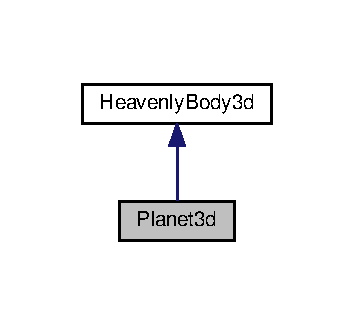
\includegraphics[width=170pt]{d7/d7e/classPlanet3d__inherit__graph}
\end{center}
\end{figure}


\-Collaboration diagram for \-Planet3d\-:\nopagebreak
\begin{figure}[H]
\begin{center}
\leavevmode
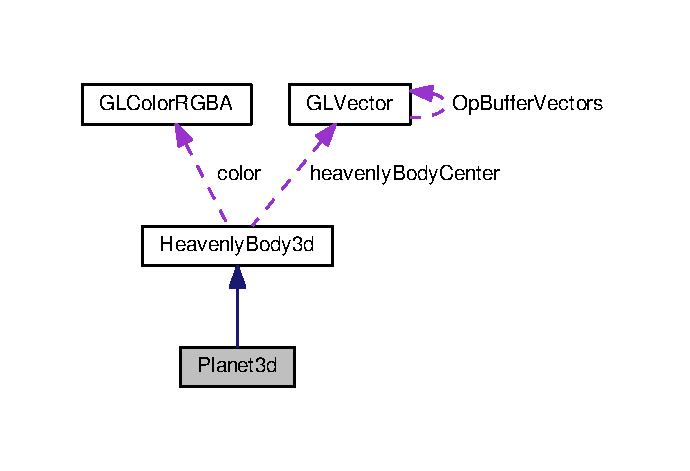
\includegraphics[width=331pt]{d2/de3/classPlanet3d__coll__graph}
\end{center}
\end{figure}
\subsection*{\-Public \-Member \-Functions}
\begin{DoxyCompactItemize}
\item 
{\bf \-Planet3d} ({\bf \-Solar\-System\-Heavenly\-Body} $\ast$solar\-System\-Heavenly\-Body, const float kepler\-Constant)
\item 
void {\bfseries paint\-Heavenly\-Body3d} ()\label{d1/d39/classPlanet3d_a2e504935919360a2015b50c103798dd8}

\item 
void {\bfseries calculate\-Heavenly\-Body3d} ()\label{d1/d39/classPlanet3d_af486055f2af946f84c309c93096596fd}

\end{DoxyCompactItemize}


\subsection{\-Detailed \-Description}
\-Der \-Abstand zwischen f\$(x\-\_\-1,y\-\_\-1)f\$ und f\$(x\-\_\-2,y\-\_\-2)f\$ ist f[sqrt\{(x\-\_\-2-\/x\-\_\-1)2+(y\-\_\-2-\/y\-\_\-1)2\}.f] 

\subsection{\-Constructor \& \-Destructor \-Documentation}
\index{\-Planet3d@{\-Planet3d}!\-Planet3d@{\-Planet3d}}
\index{\-Planet3d@{\-Planet3d}!Planet3d@{\-Planet3d}}
\subsubsection[{\-Planet3d}]{\setlength{\rightskip}{0pt plus 5cm}\-Planet3d\-::\-Planet3d (
\begin{DoxyParamCaption}
\item[{{\bf \-Solar\-System\-Heavenly\-Body} $\ast$}]{solar\-System\-Heavenly\-Body, }
\item[{const float}]{kepler\-Constant}
\end{DoxyParamCaption}
)}\label{d1/d39/classPlanet3d_ad657ee6cddb3f386e861dad977f6998c}

\begin{DoxyParams}{\-Parameters}
{\em solar\-System\-Heavenly\-Body} & \\
\hline
{\em kepler\-Constant} & \-Reference \-Value for the \-Planet speed \\
\hline
\end{DoxyParams}


\-The documentation for this class was generated from the following files\-:\begin{DoxyCompactItemize}
\item 
visualization/heavenlybody/planet3d.\-h\item 
visualization/heavenlybody/planet3d.\-cpp\end{DoxyCompactItemize}

\section{\-Postgre\-S\-Q\-L\-Database \-Class \-Reference}
\label{dc/d2c/classPostgreSQLDatabase}\index{\-Postgre\-S\-Q\-L\-Database@{\-Postgre\-S\-Q\-L\-Database}}


{\ttfamily \#include $<$postgresqldatabase.\-h$>$}

\subsection*{\-Public \-Member \-Functions}
\begin{DoxyCompactItemize}
\item 
void {\bf transaction} ()\label{dc/d2c/classPostgreSQLDatabase_a3814e1b3bfa2a3e7408a1e0855b28a45}

\begin{DoxyCompactList}\small\item\em \-Start database transaction. \end{DoxyCompactList}\item 
void {\bf commit} ()\label{dc/d2c/classPostgreSQLDatabase_a267e5394770aa97c9e410bd3c9655a36}

\begin{DoxyCompactList}\small\item\em \-Commit database operations. \end{DoxyCompactList}\item 
void {\bf rollback} ()\label{dc/d2c/classPostgreSQLDatabase_ac34287937b49aaa849627d987730ae2a}

\begin{DoxyCompactList}\small\item\em \-Rollback the database operations. \end{DoxyCompactList}\end{DoxyCompactItemize}
\subsection*{\-Static \-Public \-Member \-Functions}
\begin{DoxyCompactItemize}
\item 
static {\bf \-Postgre\-S\-Q\-L\-Database} $\ast$ {\bf get\-Instance} ()
\begin{DoxyCompactList}\small\item\em \-Make \doxyref{\-Postgre\-S\-Q\-L\-Database}{p.}{dc/d2c/classPostgreSQLDatabase} \-Object if none exists. \end{DoxyCompactList}\end{DoxyCompactItemize}
\subsection*{\-Protected \-Member \-Functions}
\begin{DoxyCompactItemize}
\item 
{\bf \-Postgre\-S\-Q\-L\-Database} ()\label{dc/d2c/classPostgreSQLDatabase_a627b4814e824226495b41ad6db182094}

\begin{DoxyCompactList}\small\item\em \-Establish database connection. \-On windows systems use \-O\-D\-B\-C, on other systems the native \-Postgre\-S\-Q\-L driver. \end{DoxyCompactList}\end{DoxyCompactItemize}


\subsection{\-Detailed \-Description}
\-Class for connect to database.

\begin{DoxyAuthor}{\-Author}
\-Fabian \-Deitelhoff $<${\tt \-F\-H@\-Fabian\-Deitelhoff.\-de}$>$ 

\-Christof \-Geisler $<${\tt christof.\-geisler@stud.\-fh-\/swf.\-de}$>$ 
\end{DoxyAuthor}


\subsection{\-Member \-Function \-Documentation}
\index{\-Postgre\-S\-Q\-L\-Database@{\-Postgre\-S\-Q\-L\-Database}!get\-Instance@{get\-Instance}}
\index{get\-Instance@{get\-Instance}!PostgreSQLDatabase@{\-Postgre\-S\-Q\-L\-Database}}
\subsubsection[{get\-Instance}]{\setlength{\rightskip}{0pt plus 5cm}{\bf \-Postgre\-S\-Q\-L\-Database} $\ast$ \-Postgre\-S\-Q\-L\-Database\-::get\-Instance (
\begin{DoxyParamCaption}
{}
\end{DoxyParamCaption}
)\hspace{0.3cm}{\ttfamily  [static]}}\label{dc/d2c/classPostgreSQLDatabase_afe0a9795acbfa2917ec3668c0ea1045b}


\-Make \doxyref{\-Postgre\-S\-Q\-L\-Database}{p.}{dc/d2c/classPostgreSQLDatabase} \-Object if none exists. 

\begin{DoxyReturn}{\-Returns}
\doxyref{\-Postgre\-S\-Q\-L\-Database}{p.}{dc/d2c/classPostgreSQLDatabase} $\ast$ \-Return the \doxyref{\-Postgre\-S\-Q\-L\-Database}{p.}{dc/d2c/classPostgreSQLDatabase} \-Object. 
\end{DoxyReturn}


\-The documentation for this class was generated from the following files\-:\begin{DoxyCompactItemize}
\item 
database/postgresqldatabase.\-h\item 
database/postgresqldatabase.\-cpp\end{DoxyCompactItemize}

\hypertarget{classPropertyNotValidException}{
\section{\-Property\-Not\-Valid\-Exception \-Class \-Reference}
\label{d8/df5/classPropertyNotValidException}\index{\-Property\-Not\-Valid\-Exception@{\-Property\-Not\-Valid\-Exception}}
}


{\ttfamily \#include $<$propertynotvalidexception.\-h$>$}

\subsection*{\-Public \-Member \-Functions}
\begin{DoxyCompactItemize}
\item 
\hyperlink{classPropertyNotValidException_a1597e12c33e8b6080dbf3bd057e03bb8}{\-Property\-Not\-Valid\-Exception} (const \-Q\-String property, const \-Q\-String message)
\begin{DoxyCompactList}\small\item\em \-Exception for non valid property. \end{DoxyCompactList}\item 
virtual \hyperlink{classPropertyNotValidException_ac44b59af3ea710aa74ca523b36bda7ff}{$\sim$\-Property\-Not\-Valid\-Exception} ()  throw ()
\item 
virtual const \-Q\-String \hyperlink{classPropertyNotValidException_a66d861efc67428d56e0196f8f5b33d26}{get\-Message} () const   throw ()
\begin{DoxyCompactList}\small\item\em \-Getter for message. \end{DoxyCompactList}\item 
virtual const \-Q\-String \hyperlink{classPropertyNotValidException_afce6ddb37d69ac02017d4f7300cdaee1}{get\-Property} () const   throw ()
\begin{DoxyCompactList}\small\item\em \-Getter foe sql\-Error. \end{DoxyCompactList}\end{DoxyCompactItemize}


\subsection{\-Detailed \-Description}
\-Class to encapsulate exceptions.

\begin{DoxyAuthor}{\-Author}
\-Fabian \-Deitelhoff $<$\href{mailto:FH@FabianDeitelhoff.de}{\tt \-F\-H@\-Fabian\-Deitelhoff.\-de}$>$ 

\-Christof \-Geisler $<$\href{mailto:christof.geisler@stud.fh-swf.de}{\tt christof.\-geisler@stud.\-fh-\/swf.\-de}$>$ 
\end{DoxyAuthor}


\subsection{\-Constructor \& \-Destructor \-Documentation}
\hypertarget{classPropertyNotValidException_a1597e12c33e8b6080dbf3bd057e03bb8}{
\index{\-Property\-Not\-Valid\-Exception@{\-Property\-Not\-Valid\-Exception}!\-Property\-Not\-Valid\-Exception@{\-Property\-Not\-Valid\-Exception}}
\index{\-Property\-Not\-Valid\-Exception@{\-Property\-Not\-Valid\-Exception}!PropertyNotValidException@{\-Property\-Not\-Valid\-Exception}}
\subsubsection[{\-Property\-Not\-Valid\-Exception}]{\setlength{\rightskip}{0pt plus 5cm}\-Property\-Not\-Valid\-Exception\-::\-Property\-Not\-Valid\-Exception (
\begin{DoxyParamCaption}
\item[{const \-Q\-String}]{property, }
\item[{const \-Q\-String}]{message}
\end{DoxyParamCaption}
)}}
\label{d8/df5/classPropertyNotValidException_a1597e12c33e8b6080dbf3bd057e03bb8}


\-Exception for non valid property. 


\begin{DoxyParams}{\-Parameters}
{\em property} & \\
\hline
{\em message} & \\
\hline
\end{DoxyParams}

\begin{DoxyCode}
{
    this->property = property;
    this->message = message.arg(property);
}
\end{DoxyCode}
\hypertarget{classPropertyNotValidException_ac44b59af3ea710aa74ca523b36bda7ff}{
\index{\-Property\-Not\-Valid\-Exception@{\-Property\-Not\-Valid\-Exception}!$\sim$\-Property\-Not\-Valid\-Exception@{$\sim$\-Property\-Not\-Valid\-Exception}}
\index{$\sim$\-Property\-Not\-Valid\-Exception@{$\sim$\-Property\-Not\-Valid\-Exception}!PropertyNotValidException@{\-Property\-Not\-Valid\-Exception}}
\subsubsection[{$\sim$\-Property\-Not\-Valid\-Exception}]{\setlength{\rightskip}{0pt plus 5cm}virtual \-Property\-Not\-Valid\-Exception\-::$\sim$\-Property\-Not\-Valid\-Exception (
\begin{DoxyParamCaption}
{}
\end{DoxyParamCaption}
)  throw ()\hspace{0.3cm}{\ttfamily  \mbox{[}inline, virtual\mbox{]}}}}
\label{d8/df5/classPropertyNotValidException_ac44b59af3ea710aa74ca523b36bda7ff}

\begin{DoxyCode}
{}
\end{DoxyCode}


\subsection{\-Member \-Function \-Documentation}
\hypertarget{classPropertyNotValidException_a66d861efc67428d56e0196f8f5b33d26}{
\index{\-Property\-Not\-Valid\-Exception@{\-Property\-Not\-Valid\-Exception}!get\-Message@{get\-Message}}
\index{get\-Message@{get\-Message}!PropertyNotValidException@{\-Property\-Not\-Valid\-Exception}}
\subsubsection[{get\-Message}]{\setlength{\rightskip}{0pt plus 5cm}const \-Q\-String \-Property\-Not\-Valid\-Exception\-::get\-Message (
\begin{DoxyParamCaption}
{}
\end{DoxyParamCaption}
) const  throw ()\hspace{0.3cm}{\ttfamily  \mbox{[}virtual\mbox{]}}}}
\label{d8/df5/classPropertyNotValidException_a66d861efc67428d56e0196f8f5b33d26}


\-Getter for message. 

\begin{DoxyReturn}{\-Returns}
const \-Q\-String 
\end{DoxyReturn}

\begin{DoxyCode}
{
    return message;
}
\end{DoxyCode}
\hypertarget{classPropertyNotValidException_afce6ddb37d69ac02017d4f7300cdaee1}{
\index{\-Property\-Not\-Valid\-Exception@{\-Property\-Not\-Valid\-Exception}!get\-Property@{get\-Property}}
\index{get\-Property@{get\-Property}!PropertyNotValidException@{\-Property\-Not\-Valid\-Exception}}
\subsubsection[{get\-Property}]{\setlength{\rightskip}{0pt plus 5cm}const \-Q\-String \-Property\-Not\-Valid\-Exception\-::get\-Property (
\begin{DoxyParamCaption}
{}
\end{DoxyParamCaption}
) const  throw ()\hspace{0.3cm}{\ttfamily  \mbox{[}virtual\mbox{]}}}}
\label{d8/df5/classPropertyNotValidException_afce6ddb37d69ac02017d4f7300cdaee1}


\-Getter foe sql\-Error. 

\begin{DoxyReturn}{\-Returns}
const \-Q\-String 
\end{DoxyReturn}

\begin{DoxyCode}
{
    return property;
}
\end{DoxyCode}


\-The documentation for this class was generated from the following files\-:\begin{DoxyCompactItemize}
\item 
model/exceptions/\hyperlink{propertynotvalidexception_8h}{propertynotvalidexception.\-h}\item 
model/exceptions/\hyperlink{propertynotvalidexception_8cpp}{propertynotvalidexception.\-cpp}\end{DoxyCompactItemize}

\hypertarget{classSimulationView}{
\section{\-Simulation\-View \-Class \-Reference}
\label{d9/df6/classSimulationView}\index{\-Simulation\-View@{\-Simulation\-View}}
}


{\ttfamily \#include $<$simulationview.\-h$>$}

\subsection*{\-Signals}
\begin{DoxyCompactItemize}
\item 
void \hyperlink{classSimulationView_a4198d47f7517525c5702a9bc6e1e9369}{simulation\-Stopped} ()
\item 
void \hyperlink{classSimulationView_ac6d069baef5c77cff2b8ada065950ab4}{collision\-Detection\-Deactivated} ()
\end{DoxyCompactItemize}
\subsection*{\-Public \-Member \-Functions}
\begin{DoxyCompactItemize}
\item 
\hyperlink{classSimulationView_a4d55de963f5612a2c894f501a8928991}{\-Simulation\-View} (\-Q\-Widget $\ast$parent=0, \hyperlink{classSolarSystemSimulation}{\-Solar\-System\-Simulation} $\ast$solar\-System\-Simulation=0)
\begin{DoxyCompactList}\small\item\em \-Class to show the scene, move the camera and initialize the simulation view. \end{DoxyCompactList}\item 
\hyperlink{classSimulationView_a7ccb9a29e3632431bba5a686da61d8a9}{$\sim$\-Simulation\-View} ()
\begin{DoxyCompactList}\small\item\em \-Destructor for the view. \end{DoxyCompactList}\item 
void \hyperlink{classSimulationView_ad1e431046ff2a7e774d92bbba6fded3b}{set\-Solar\-System} (\hyperlink{classSolarSystem}{\-Solar\-System} $\ast$solar\-System)
\begin{DoxyCompactList}\small\item\em \-Init the simulation. \end{DoxyCompactList}\item 
void \hyperlink{classSimulationView_ae7936c84b92f7ae64a772a9ba1422624}{start\-Simulation} ()
\begin{DoxyCompactList}\small\item\em \-Starts the timer for the timer event. \end{DoxyCompactList}\item 
void \hyperlink{classSimulationView_ad51d8480373e82c73e3353c868df6f87}{stop\-Simulation} ()
\begin{DoxyCompactList}\small\item\em \-Freeze the simulation. \end{DoxyCompactList}\item 
void \hyperlink{classSimulationView_acde2b2fb1ac01e85a8f8efbbe6717f12}{reset\-Perspective} ()
\begin{DoxyCompactList}\small\item\em \-Resets the perspective of the scene. \end{DoxyCompactList}\item 
bool \hyperlink{classSimulationView_a20413dcac5bc5d52b9d5fae836cf3f93}{is\-Simulation\-Started} ()
\begin{DoxyCompactList}\small\item\em \-Get the status of the timer. \end{DoxyCompactList}\item 
void \hyperlink{classSimulationView_a712a4c812faec9a14699c1ceb1048337}{toggle\-Coordinate\-Axes\-Visibility} ()
\begin{DoxyCompactList}\small\item\em \-Toggle visibility of coordinates and redraw scene. \end{DoxyCompactList}\end{DoxyCompactItemize}
\subsection*{\-Protected \-Member \-Functions}
\begin{DoxyCompactItemize}
\item 
void \hyperlink{classSimulationView_aabf60efd5011c63555e9bd154107f42d}{key\-Press\-Event} (\-Q\-Key\-Event $\ast$key\-Event)
\begin{DoxyCompactList}\small\item\em \-Key detection to turn around and shift the scene. \end{DoxyCompactList}\end{DoxyCompactItemize}


\subsection{\-Detailed \-Description}
\-Class with components to show and administrate the simulation view window.

\begin{DoxyAuthor}{\-Author}
\-Fabian \-Deitelhoff $<$\href{mailto:FH@FabianDeitelhoff.de}{\tt \-F\-H@\-Fabian\-Deitelhoff.\-de}$>$ 

\-Christof \-Geisler $<$\href{mailto:christof.geisler@stud.fh-swf.de}{\tt christof.\-geisler@stud.\-fh-\/swf.\-de}$>$ 
\end{DoxyAuthor}


\subsection{\-Constructor \& \-Destructor \-Documentation}
\hypertarget{classSimulationView_a4d55de963f5612a2c894f501a8928991}{
\index{\-Simulation\-View@{\-Simulation\-View}!\-Simulation\-View@{\-Simulation\-View}}
\index{\-Simulation\-View@{\-Simulation\-View}!SimulationView@{\-Simulation\-View}}
\subsubsection[{\-Simulation\-View}]{\setlength{\rightskip}{0pt plus 5cm}\-Simulation\-View\-::\-Simulation\-View (
\begin{DoxyParamCaption}
\item[{\-Q\-Widget $\ast$}]{parent = {\ttfamily 0}, }
\item[{{\bf \-Solar\-System\-Simulation} $\ast$}]{solar\-System\-Simulation = {\ttfamily 0}}
\end{DoxyParamCaption}
)\hspace{0.3cm}{\ttfamily  \mbox{[}explicit\mbox{]}}}}
\label{d9/df6/classSimulationView_a4d55de963f5612a2c894f501a8928991}


\-Class to show the scene, move the camera and initialize the simulation view. 


\begin{DoxyParams}{\-Parameters}
{\em parent} & \\
\hline
{\em solar\-System\-Simulation} & \\
\hline
\end{DoxyParams}

\begin{DoxyCode}
                                                                               
                   :
    QGLWidget(parent)
{
    perspective = new GLPerspective();

    light = new Light();

    environment = new Environment();

    setFocusPolicy(Qt::StrongFocus);
    setMouseTracking(true);

    this->solarSystemSimulation = solarSystemSimulation;
    connect(solarSystemSimulation,
            SIGNAL(collisionDetected(HeavenlyBody3d*,HeavenlyBody3d*)),
            this,
            SLOT(collisionDetected(HeavenlyBody3d*,HeavenlyBody3d*)));

    timer = new QTimer(this);
    connect(timer,
            SIGNAL(timeout()),
            this,
            SLOT(timerEvent()));

    // Some initial constants for the camera position and control.
    cameraZFactor = 3.5;
    axisLengthFactor = 2.0;
    backgroundColor = Qt::black;
    shiftSceneUpDownFactor = 0.5;
    shiftSceneLeftRightFactor = 0.5;
    shiftSceneForwardBackwardFactor = 1.0;
    turnCameraUpDownFactor = 1.0;
    turnCameraLeftRightFactor = 1.0;
    stretchCameraDistanceForwardFactor = 0.85;
    stretchCameraDistanceBackwardFactor = 1.15;
}
\end{DoxyCode}
\hypertarget{classSimulationView_a7ccb9a29e3632431bba5a686da61d8a9}{
\index{\-Simulation\-View@{\-Simulation\-View}!$\sim$\-Simulation\-View@{$\sim$\-Simulation\-View}}
\index{$\sim$\-Simulation\-View@{$\sim$\-Simulation\-View}!SimulationView@{\-Simulation\-View}}
\subsubsection[{$\sim$\-Simulation\-View}]{\setlength{\rightskip}{0pt plus 5cm}\-Simulation\-View\-::$\sim$\-Simulation\-View (
\begin{DoxyParamCaption}
{}
\end{DoxyParamCaption}
)}}
\label{d9/df6/classSimulationView_a7ccb9a29e3632431bba5a686da61d8a9}


\-Destructor for the view. 


\begin{DoxyCode}
{
    stopSimulation();

    delete perspective;
    delete light;
    delete environment;
    delete timer;
}
\end{DoxyCode}


\subsection{\-Member \-Function \-Documentation}
\hypertarget{classSimulationView_ac6d069baef5c77cff2b8ada065950ab4}{
\index{\-Simulation\-View@{\-Simulation\-View}!collision\-Detection\-Deactivated@{collision\-Detection\-Deactivated}}
\index{collision\-Detection\-Deactivated@{collision\-Detection\-Deactivated}!SimulationView@{\-Simulation\-View}}
\subsubsection[{collision\-Detection\-Deactivated}]{\setlength{\rightskip}{0pt plus 5cm}void \-Simulation\-View\-::collision\-Detection\-Deactivated (
\begin{DoxyParamCaption}
{}
\end{DoxyParamCaption}
)\hspace{0.3cm}{\ttfamily  \mbox{[}signal\mbox{]}}}}
\label{d9/df6/classSimulationView_ac6d069baef5c77cff2b8ada065950ab4}
\hypertarget{classSimulationView_a20413dcac5bc5d52b9d5fae836cf3f93}{
\index{\-Simulation\-View@{\-Simulation\-View}!is\-Simulation\-Started@{is\-Simulation\-Started}}
\index{is\-Simulation\-Started@{is\-Simulation\-Started}!SimulationView@{\-Simulation\-View}}
\subsubsection[{is\-Simulation\-Started}]{\setlength{\rightskip}{0pt plus 5cm}bool \-Simulation\-View\-::is\-Simulation\-Started (
\begin{DoxyParamCaption}
{}
\end{DoxyParamCaption}
)}}
\label{d9/df6/classSimulationView_a20413dcac5bc5d52b9d5fae836cf3f93}


\-Get the status of the timer. 

\begin{DoxyReturn}{\-Returns}
bool 
\end{DoxyReturn}

\begin{DoxyCode}
{
    return timer->isActive();
}
\end{DoxyCode}
\hypertarget{classSimulationView_aabf60efd5011c63555e9bd154107f42d}{
\index{\-Simulation\-View@{\-Simulation\-View}!key\-Press\-Event@{key\-Press\-Event}}
\index{key\-Press\-Event@{key\-Press\-Event}!SimulationView@{\-Simulation\-View}}
\subsubsection[{key\-Press\-Event}]{\setlength{\rightskip}{0pt plus 5cm}void \-Simulation\-View\-::key\-Press\-Event (
\begin{DoxyParamCaption}
\item[{\-Q\-Key\-Event $\ast$}]{key\-Event}
\end{DoxyParamCaption}
)\hspace{0.3cm}{\ttfamily  \mbox{[}protected\mbox{]}}}}
\label{d9/df6/classSimulationView_aabf60efd5011c63555e9bd154107f42d}


\-Key detection to turn around and shift the scene. 


\begin{DoxyParams}{\-Parameters}
{\em key\-Event} & \\
\hline
\end{DoxyParams}

\begin{DoxyCode}
{
    Qt::KeyboardModifiers modifiers = keyEvent->modifiers();
    // Is the CTRL key pressed?
    if (modifiers & Qt::ControlModifier)
    {
        // Is the windows or the alt key pressed.
        if (modifiers & Qt::MetaModifier || modifiers & Qt::AltModifier)
        {
            switch (keyEvent->key())
            {
            case Qt::Key_Up:
                turnCameraUpDown(turnCameraUpDownFactor);
                break;
            case Qt::Key_Down:
                turnCameraUpDown(-turnCameraUpDownFactor);
                break;
            case Qt::Key_Left:
                turnCameraLeftRight(turnCameraLeftRightFactor);
                break;
            case Qt::Key_Right:
                turnCameraLeftRight(-turnCameraLeftRightFactor);
                break;
            case Qt::Key_PageDown:
                stretchCameraDistance(stretchCameraDistanceBackwardFactor);
                break;
            case Qt::Key_PageUp:
                stretchCameraDistance(stretchCameraDistanceForwardFactor);
                break;
            default:
                break;
            }
        }

        // Is the SHIFT key pressed?
        if (modifiers & Qt::ShiftModifier)
        {
            switch (keyEvent->key())
            {
            case Qt::Key_Up:
                shiftSceneUpDown(-shiftSceneUpDownFactor);
                break;
            case Qt::Key_Down:
                shiftSceneUpDown(shiftSceneUpDownFactor);
                break;
            case Qt::Key_Left:
                shiftSceneLeftRight(shiftSceneLeftRightFactor);
                break;
            case Qt::Key_Right:
                shiftSceneLeftRight(-shiftSceneLeftRightFactor);
                break;
            case Qt::Key_PageDown:
                stretchCameraDistance(stretchCameraDistanceBackwardFactor);
                break;
            case Qt::Key_PageUp:
                stretchCameraDistance(stretchCameraDistanceForwardFactor);
                break;
            default:
                break;
            }
        }
    }

    updateOpenGL();
}
\end{DoxyCode}
\hypertarget{classSimulationView_acde2b2fb1ac01e85a8f8efbbe6717f12}{
\index{\-Simulation\-View@{\-Simulation\-View}!reset\-Perspective@{reset\-Perspective}}
\index{reset\-Perspective@{reset\-Perspective}!SimulationView@{\-Simulation\-View}}
\subsubsection[{reset\-Perspective}]{\setlength{\rightskip}{0pt plus 5cm}void \-Simulation\-View\-::reset\-Perspective (
\begin{DoxyParamCaption}
{}
\end{DoxyParamCaption}
)}}
\label{d9/df6/classSimulationView_acde2b2fb1ac01e85a8f8efbbe6717f12}


\-Resets the perspective of the scene. 


\begin{DoxyCode}
{
    perspective->setCamera(solarSystemSimulation->getMaxSemimajorAxis() * 
      cameraZFactor * v_Z);
    perspective->setCenter(v_Zero);
    axisLength = perspective->distance() * axisLengthFactor;
}
\end{DoxyCode}
\hypertarget{classSimulationView_ad1e431046ff2a7e774d92bbba6fded3b}{
\index{\-Simulation\-View@{\-Simulation\-View}!set\-Solar\-System@{set\-Solar\-System}}
\index{set\-Solar\-System@{set\-Solar\-System}!SimulationView@{\-Simulation\-View}}
\subsubsection[{set\-Solar\-System}]{\setlength{\rightskip}{0pt plus 5cm}void \-Simulation\-View\-::set\-Solar\-System (
\begin{DoxyParamCaption}
\item[{{\bf \-Solar\-System} $\ast$}]{solar\-System}
\end{DoxyParamCaption}
)}}
\label{d9/df6/classSimulationView_ad1e431046ff2a7e774d92bbba6fded3b}


\-Init the simulation. 


\begin{DoxyParams}{\-Parameters}
{\em solar\-System} & \\
\hline
\end{DoxyParams}

\begin{DoxyCode}
{
    solarSystemSimulation->setSolarSystem(solarSystem);
    resetPerspective();
}
\end{DoxyCode}
\hypertarget{classSimulationView_a4198d47f7517525c5702a9bc6e1e9369}{
\index{\-Simulation\-View@{\-Simulation\-View}!simulation\-Stopped@{simulation\-Stopped}}
\index{simulation\-Stopped@{simulation\-Stopped}!SimulationView@{\-Simulation\-View}}
\subsubsection[{simulation\-Stopped}]{\setlength{\rightskip}{0pt plus 5cm}void \-Simulation\-View\-::simulation\-Stopped (
\begin{DoxyParamCaption}
{}
\end{DoxyParamCaption}
)\hspace{0.3cm}{\ttfamily  \mbox{[}signal\mbox{]}}}}
\label{d9/df6/classSimulationView_a4198d47f7517525c5702a9bc6e1e9369}
\hypertarget{classSimulationView_ae7936c84b92f7ae64a772a9ba1422624}{
\index{\-Simulation\-View@{\-Simulation\-View}!start\-Simulation@{start\-Simulation}}
\index{start\-Simulation@{start\-Simulation}!SimulationView@{\-Simulation\-View}}
\subsubsection[{start\-Simulation}]{\setlength{\rightskip}{0pt plus 5cm}void \-Simulation\-View\-::start\-Simulation (
\begin{DoxyParamCaption}
{}
\end{DoxyParamCaption}
)}}
\label{d9/df6/classSimulationView_ae7936c84b92f7ae64a772a9ba1422624}


\-Starts the timer for the timer event. 


\begin{DoxyCode}
{
    if (!timer->isActive())
    {
        timer->start(10);
    }
}
\end{DoxyCode}
\hypertarget{classSimulationView_ad51d8480373e82c73e3353c868df6f87}{
\index{\-Simulation\-View@{\-Simulation\-View}!stop\-Simulation@{stop\-Simulation}}
\index{stop\-Simulation@{stop\-Simulation}!SimulationView@{\-Simulation\-View}}
\subsubsection[{stop\-Simulation}]{\setlength{\rightskip}{0pt plus 5cm}void \-Simulation\-View\-::stop\-Simulation (
\begin{DoxyParamCaption}
{}
\end{DoxyParamCaption}
)}}
\label{d9/df6/classSimulationView_ad51d8480373e82c73e3353c868df6f87}


\-Freeze the simulation. 


\begin{DoxyCode}
{
    if (timer->isActive())
    {
        timer->stop();
        emit simulationStopped();
    }
}
\end{DoxyCode}
\hypertarget{classSimulationView_a712a4c812faec9a14699c1ceb1048337}{
\index{\-Simulation\-View@{\-Simulation\-View}!toggle\-Coordinate\-Axes\-Visibility@{toggle\-Coordinate\-Axes\-Visibility}}
\index{toggle\-Coordinate\-Axes\-Visibility@{toggle\-Coordinate\-Axes\-Visibility}!SimulationView@{\-Simulation\-View}}
\subsubsection[{toggle\-Coordinate\-Axes\-Visibility}]{\setlength{\rightskip}{0pt plus 5cm}void \-Simulation\-View\-::toggle\-Coordinate\-Axes\-Visibility (
\begin{DoxyParamCaption}
{}
\end{DoxyParamCaption}
)}}
\label{d9/df6/classSimulationView_a712a4c812faec9a14699c1ceb1048337}


\-Toggle visibility of coordinates and redraw scene. 


\begin{DoxyCode}
{
    environment->toggleCoordinateAxesVisibility();

    update();
}
\end{DoxyCode}


\-The documentation for this class was generated from the following files\-:\begin{DoxyCompactItemize}
\item 
forms/simulation/\hyperlink{simulationview_8h}{simulationview.\-h}\item 
forms/simulation/\hyperlink{simulationview_8cpp}{simulationview.\-cpp}\end{DoxyCompactItemize}

\hypertarget{classSolarSystem}{
\section{\-Solar\-System \-Class \-Reference}
\label{df/d5e/classSolarSystem}\index{\-Solar\-System@{\-Solar\-System}}
}


{\ttfamily \#include $<$solarsystem.\-h$>$}

\subsection*{\-Public \-Member \-Functions}
\begin{DoxyCompactItemize}
\item 
\hyperlink{classSolarSystem_acd1c223637e498a57d8cee6593f69137}{\-Solar\-System} (\-Q\-String name, \hyperlink{classHeavenlyBody}{\-Heavenly\-Body} $\ast$central\-Star)
\begin{DoxyCompactList}\small\item\em \-Constructor for solar system with name and central star. \end{DoxyCompactList}\item 
\hyperlink{classSolarSystem_afa3e85e6ab9fbe04e2cb80dc02c69dfc}{\-Solar\-System} (qint64 id, \-Q\-String name, \hyperlink{classHeavenlyBody}{\-Heavenly\-Body} $\ast$central\-Star)
\begin{DoxyCompactList}\small\item\em \-Constructor for solar system with id, name and central star. \end{DoxyCompactList}\item 
void \hyperlink{classSolarSystem_a051c4da538ac4a9495e775e60855786e}{init} (\-Q\-String name, \hyperlink{classHeavenlyBody}{\-Heavenly\-Body} $\ast$central\-Star)
\begin{DoxyCompactList}\small\item\em \-Method to init the solar system with a name and a central star. \end{DoxyCompactList}\item 
qint64 \hyperlink{classSolarSystem_a6d73dac11e01ecf06906ede55e8b77fc}{get\-Id} ()
\begin{DoxyCompactList}\small\item\em \-Getter for the id. \end{DoxyCompactList}\item 
\-Q\-String \hyperlink{classSolarSystem_a46abe6f8ea2f1db709d3fac9f1bbf00d}{get\-Name} ()
\begin{DoxyCompactList}\small\item\em \-Getter for the name. \end{DoxyCompactList}\item 
\hyperlink{classHeavenlyBody}{\-Heavenly\-Body} $\ast$ \hyperlink{classSolarSystem_a90d1c7f9e05a1bd528b62056b27ff424}{get\-Central\-Star} ()
\begin{DoxyCompactList}\small\item\em \-Getter for the central star. \end{DoxyCompactList}\item 
int \hyperlink{classSolarSystem_a2b6d483d05a984f94c2916f41d812f4b}{get\-Planet\-Count} ()
\begin{DoxyCompactList}\small\item\em \-Getter for the number of heavenly bodies. \end{DoxyCompactList}\item 
\-Q\-List$<$ \hyperlink{classSolarSystemHeavenlyBody}{\-Solar\-System\-Heavenly\-Body} $\ast$ $>$ \hyperlink{classSolarSystem_ad9adea29a8b57fe361591cafce61b0e2}{get\-Heavenly\-Bodies} ()
\begin{DoxyCompactList}\small\item\em \-Getter for the list of heavenly bodies. \end{DoxyCompactList}\item 
void \hyperlink{classSolarSystem_a97a3b70024c266b428cf4bea2ecdb45c}{set\-Id} (qint64 id)
\begin{DoxyCompactList}\small\item\em \-Setter for the id. \end{DoxyCompactList}\item 
void \hyperlink{classSolarSystem_a1642e94eaa54bc4e43471384f95dcc7d}{set\-Name} (\-Q\-String name)
\begin{DoxyCompactList}\small\item\em \-Setter for the name. \end{DoxyCompactList}\item 
void \hyperlink{classSolarSystem_a468b93dfe340aff47ae7a010020ca365}{set\-Central\-Star} (\hyperlink{classHeavenlyBody}{\-Heavenly\-Body} $\ast$central\-Star)
\begin{DoxyCompactList}\small\item\em \-Setter for the central star. \end{DoxyCompactList}\item 
void \hyperlink{classSolarSystem_abb8b63f463e770dcd596a5df020ec4be}{add\-Heavenly\-Body} (\hyperlink{classSolarSystemHeavenlyBody}{\-Solar\-System\-Heavenly\-Body} $\ast$solar\-System\-Heavenly\-Body)
\begin{DoxyCompactList}\small\item\em \-Add a heavenly body to the solar system. \end{DoxyCompactList}\item 
void \hyperlink{classSolarSystem_a20851d16c7fac4274206834c11746b13}{remove\-Heavenly\-Body} (\hyperlink{classSolarSystemHeavenlyBody}{\-Solar\-System\-Heavenly\-Body} $\ast$solar\-System\-Heavenly\-Body)
\begin{DoxyCompactList}\small\item\em \-Remove a heavenly body from the solar system. \end{DoxyCompactList}\end{DoxyCompactItemize}


\subsection{\-Detailed \-Description}
\-Class to model a solar system.

\begin{DoxyAuthor}{\-Author}
\-Fabian \-Deitelhoff $<$\href{mailto:FH@FabianDeitelhoff.de}{\tt \-F\-H@\-Fabian\-Deitelhoff.\-de}$>$ 

\-Christof \-Geisler $<$\href{mailto:christof.geisler@stud.fh-swf.de}{\tt christof.\-geisler@stud.\-fh-\/swf.\-de}$>$ 
\end{DoxyAuthor}


\subsection{\-Constructor \& \-Destructor \-Documentation}
\hypertarget{classSolarSystem_acd1c223637e498a57d8cee6593f69137}{
\index{\-Solar\-System@{\-Solar\-System}!\-Solar\-System@{\-Solar\-System}}
\index{\-Solar\-System@{\-Solar\-System}!SolarSystem@{\-Solar\-System}}
\subsubsection[{\-Solar\-System}]{\setlength{\rightskip}{0pt plus 5cm}\-Solar\-System\-::\-Solar\-System (
\begin{DoxyParamCaption}
\item[{\-Q\-String}]{name, }
\item[{{\bf \-Heavenly\-Body} $\ast$}]{central\-Star}
\end{DoxyParamCaption}
)}}
\label{df/d5e/classSolarSystem_acd1c223637e498a57d8cee6593f69137}


\-Constructor for solar system with name and central star. 


\begin{DoxyParams}{\-Parameters}
{\em name} & \\
\hline
{\em central\-Star} & \\
\hline
\end{DoxyParams}

\begin{DoxyCode}
{
    id = -1;

    init(name, centralStar);
}
\end{DoxyCode}
\hypertarget{classSolarSystem_afa3e85e6ab9fbe04e2cb80dc02c69dfc}{
\index{\-Solar\-System@{\-Solar\-System}!\-Solar\-System@{\-Solar\-System}}
\index{\-Solar\-System@{\-Solar\-System}!SolarSystem@{\-Solar\-System}}
\subsubsection[{\-Solar\-System}]{\setlength{\rightskip}{0pt plus 5cm}\-Solar\-System\-::\-Solar\-System (
\begin{DoxyParamCaption}
\item[{qint64}]{id, }
\item[{\-Q\-String}]{name, }
\item[{{\bf \-Heavenly\-Body} $\ast$}]{central\-Star}
\end{DoxyParamCaption}
)}}
\label{df/d5e/classSolarSystem_afa3e85e6ab9fbe04e2cb80dc02c69dfc}


\-Constructor for solar system with id, name and central star. 


\begin{DoxyParams}{\-Parameters}
{\em id} & \\
\hline
{\em name} & \\
\hline
{\em central\-Star} & \\
\hline
\end{DoxyParams}

\begin{DoxyCode}
{
    setId(id);

    init(name, centralStar);
}
\end{DoxyCode}


\subsection{\-Member \-Function \-Documentation}
\hypertarget{classSolarSystem_abb8b63f463e770dcd596a5df020ec4be}{
\index{\-Solar\-System@{\-Solar\-System}!add\-Heavenly\-Body@{add\-Heavenly\-Body}}
\index{add\-Heavenly\-Body@{add\-Heavenly\-Body}!SolarSystem@{\-Solar\-System}}
\subsubsection[{add\-Heavenly\-Body}]{\setlength{\rightskip}{0pt plus 5cm}void \-Solar\-System\-::add\-Heavenly\-Body (
\begin{DoxyParamCaption}
\item[{{\bf \-Solar\-System\-Heavenly\-Body} $\ast$}]{solar\-System\-Heavenly\-Body}
\end{DoxyParamCaption}
)}}
\label{df/d5e/classSolarSystem_abb8b63f463e770dcd596a5df020ec4be}


\-Add a heavenly body to the solar system. 


\begin{DoxyParams}{\-Parameters}
{\em solar\-System\-Heavenly\-Body} & \\
\hline
\end{DoxyParams}

\begin{DoxyCode}
{
    if (solarSystemHeavenlyBody)
    {
        heavenlyBodies.append(solarSystemHeavenlyBody);
    }
}
\end{DoxyCode}
\hypertarget{classSolarSystem_a90d1c7f9e05a1bd528b62056b27ff424}{
\index{\-Solar\-System@{\-Solar\-System}!get\-Central\-Star@{get\-Central\-Star}}
\index{get\-Central\-Star@{get\-Central\-Star}!SolarSystem@{\-Solar\-System}}
\subsubsection[{get\-Central\-Star}]{\setlength{\rightskip}{0pt plus 5cm}{\bf \-Heavenly\-Body}$\ast$ \-Solar\-System\-::get\-Central\-Star (
\begin{DoxyParamCaption}
{}
\end{DoxyParamCaption}
)\hspace{0.3cm}{\ttfamily  \mbox{[}inline\mbox{]}}}}
\label{df/d5e/classSolarSystem_a90d1c7f9e05a1bd528b62056b27ff424}


\-Getter for the central star. 

\begin{DoxyReturn}{\-Returns}
\hyperlink{classHeavenlyBody}{\-Heavenly\-Body} $\ast$ 
\end{DoxyReturn}

\begin{DoxyCode}
{ return centralStar; }
\end{DoxyCode}
\hypertarget{classSolarSystem_ad9adea29a8b57fe361591cafce61b0e2}{
\index{\-Solar\-System@{\-Solar\-System}!get\-Heavenly\-Bodies@{get\-Heavenly\-Bodies}}
\index{get\-Heavenly\-Bodies@{get\-Heavenly\-Bodies}!SolarSystem@{\-Solar\-System}}
\subsubsection[{get\-Heavenly\-Bodies}]{\setlength{\rightskip}{0pt plus 5cm}\-Q\-List$<${\bf \-Solar\-System\-Heavenly\-Body} $\ast$$>$ \-Solar\-System\-::get\-Heavenly\-Bodies (
\begin{DoxyParamCaption}
{}
\end{DoxyParamCaption}
)\hspace{0.3cm}{\ttfamily  \mbox{[}inline\mbox{]}}}}
\label{df/d5e/classSolarSystem_ad9adea29a8b57fe361591cafce61b0e2}


\-Getter for the list of heavenly bodies. 

\begin{DoxyReturn}{\-Returns}
\-Q\-List$<$\-Solar\-System\-Heavenly\-Body $\ast$$>$ 
\end{DoxyReturn}

\begin{DoxyCode}
{ return heavenlyBodies; }
\end{DoxyCode}
\hypertarget{classSolarSystem_a6d73dac11e01ecf06906ede55e8b77fc}{
\index{\-Solar\-System@{\-Solar\-System}!get\-Id@{get\-Id}}
\index{get\-Id@{get\-Id}!SolarSystem@{\-Solar\-System}}
\subsubsection[{get\-Id}]{\setlength{\rightskip}{0pt plus 5cm}qint64 \-Solar\-System\-::get\-Id (
\begin{DoxyParamCaption}
{}
\end{DoxyParamCaption}
)\hspace{0.3cm}{\ttfamily  \mbox{[}inline\mbox{]}}}}
\label{df/d5e/classSolarSystem_a6d73dac11e01ecf06906ede55e8b77fc}


\-Getter for the id. 

\begin{DoxyReturn}{\-Returns}
qint64 
\end{DoxyReturn}

\begin{DoxyCode}
{ return id; }
\end{DoxyCode}
\hypertarget{classSolarSystem_a46abe6f8ea2f1db709d3fac9f1bbf00d}{
\index{\-Solar\-System@{\-Solar\-System}!get\-Name@{get\-Name}}
\index{get\-Name@{get\-Name}!SolarSystem@{\-Solar\-System}}
\subsubsection[{get\-Name}]{\setlength{\rightskip}{0pt plus 5cm}\-Q\-String \-Solar\-System\-::get\-Name (
\begin{DoxyParamCaption}
{}
\end{DoxyParamCaption}
)\hspace{0.3cm}{\ttfamily  \mbox{[}inline\mbox{]}}}}
\label{df/d5e/classSolarSystem_a46abe6f8ea2f1db709d3fac9f1bbf00d}


\-Getter for the name. 

\begin{DoxyReturn}{\-Returns}
\-Q\-String 
\end{DoxyReturn}

\begin{DoxyCode}
{ return name; }
\end{DoxyCode}
\hypertarget{classSolarSystem_a2b6d483d05a984f94c2916f41d812f4b}{
\index{\-Solar\-System@{\-Solar\-System}!get\-Planet\-Count@{get\-Planet\-Count}}
\index{get\-Planet\-Count@{get\-Planet\-Count}!SolarSystem@{\-Solar\-System}}
\subsubsection[{get\-Planet\-Count}]{\setlength{\rightskip}{0pt plus 5cm}int \-Solar\-System\-::get\-Planet\-Count (
\begin{DoxyParamCaption}
{}
\end{DoxyParamCaption}
)\hspace{0.3cm}{\ttfamily  \mbox{[}inline\mbox{]}}}}
\label{df/d5e/classSolarSystem_a2b6d483d05a984f94c2916f41d812f4b}


\-Getter for the number of heavenly bodies. 

\begin{DoxyReturn}{\-Returns}
int 
\end{DoxyReturn}

\begin{DoxyCode}
{ return heavenlyBodies.size(); }
\end{DoxyCode}
\hypertarget{classSolarSystem_a051c4da538ac4a9495e775e60855786e}{
\index{\-Solar\-System@{\-Solar\-System}!init@{init}}
\index{init@{init}!SolarSystem@{\-Solar\-System}}
\subsubsection[{init}]{\setlength{\rightskip}{0pt plus 5cm}void \-Solar\-System\-::init (
\begin{DoxyParamCaption}
\item[{\-Q\-String}]{name, }
\item[{{\bf \-Heavenly\-Body} $\ast$}]{central\-Star}
\end{DoxyParamCaption}
)}}
\label{df/d5e/classSolarSystem_a051c4da538ac4a9495e775e60855786e}


\-Method to init the solar system with a name and a central star. 


\begin{DoxyParams}{\-Parameters}
{\em name} & \\
\hline
{\em central\-Star} & \\
\hline
\end{DoxyParams}

\begin{DoxyCode}
{
    setName(name);
    setCentralStar(centralStar);
}
\end{DoxyCode}
\hypertarget{classSolarSystem_a20851d16c7fac4274206834c11746b13}{
\index{\-Solar\-System@{\-Solar\-System}!remove\-Heavenly\-Body@{remove\-Heavenly\-Body}}
\index{remove\-Heavenly\-Body@{remove\-Heavenly\-Body}!SolarSystem@{\-Solar\-System}}
\subsubsection[{remove\-Heavenly\-Body}]{\setlength{\rightskip}{0pt plus 5cm}void \-Solar\-System\-::remove\-Heavenly\-Body (
\begin{DoxyParamCaption}
\item[{{\bf \-Solar\-System\-Heavenly\-Body} $\ast$}]{solar\-System\-Heavenly\-Body}
\end{DoxyParamCaption}
)}}
\label{df/d5e/classSolarSystem_a20851d16c7fac4274206834c11746b13}


\-Remove a heavenly body from the solar system. 


\begin{DoxyParams}{\-Parameters}
{\em solar\-System\-Heavenly\-Body} & \\
\hline
\end{DoxyParams}

\begin{DoxyCode}
{
    if (solarSystemHeavenlyBody)
    {
        heavenlyBodies.removeOne(solarSystemHeavenlyBody);
    }
}
\end{DoxyCode}
\hypertarget{classSolarSystem_a468b93dfe340aff47ae7a010020ca365}{
\index{\-Solar\-System@{\-Solar\-System}!set\-Central\-Star@{set\-Central\-Star}}
\index{set\-Central\-Star@{set\-Central\-Star}!SolarSystem@{\-Solar\-System}}
\subsubsection[{set\-Central\-Star}]{\setlength{\rightskip}{0pt plus 5cm}void \-Solar\-System\-::set\-Central\-Star (
\begin{DoxyParamCaption}
\item[{{\bf \-Heavenly\-Body} $\ast$}]{central\-Star}
\end{DoxyParamCaption}
)}}
\label{df/d5e/classSolarSystem_a468b93dfe340aff47ae7a010020ca365}


\-Setter for the central star. 


\begin{DoxyParams}{\-Parameters}
{\em central\-Star} & \\
\hline
\end{DoxyParams}

\begin{DoxyCode}
{
    if (!centralStar)
    {
        throw PropertyNotValidException("CentralStar", "The field '%1' must be
       a valid central star!");
    }

    this->centralStar = centralStar;
}
\end{DoxyCode}
\hypertarget{classSolarSystem_a97a3b70024c266b428cf4bea2ecdb45c}{
\index{\-Solar\-System@{\-Solar\-System}!set\-Id@{set\-Id}}
\index{set\-Id@{set\-Id}!SolarSystem@{\-Solar\-System}}
\subsubsection[{set\-Id}]{\setlength{\rightskip}{0pt plus 5cm}void \-Solar\-System\-::set\-Id (
\begin{DoxyParamCaption}
\item[{qint64}]{id}
\end{DoxyParamCaption}
)}}
\label{df/d5e/classSolarSystem_a97a3b70024c266b428cf4bea2ecdb45c}


\-Setter for the id. 


\begin{DoxyParams}{\-Parameters}
{\em id} & \\
\hline
\end{DoxyParams}

\begin{DoxyCode}
{
    if (id < 1)
    {
        throw PropertyNotValidException("ID", "The field '%1' has to be larger
       than 0!");
    }

    this->id = id;
}
\end{DoxyCode}
\hypertarget{classSolarSystem_a1642e94eaa54bc4e43471384f95dcc7d}{
\index{\-Solar\-System@{\-Solar\-System}!set\-Name@{set\-Name}}
\index{set\-Name@{set\-Name}!SolarSystem@{\-Solar\-System}}
\subsubsection[{set\-Name}]{\setlength{\rightskip}{0pt plus 5cm}void \-Solar\-System\-::set\-Name (
\begin{DoxyParamCaption}
\item[{\-Q\-String}]{name}
\end{DoxyParamCaption}
)}}
\label{df/d5e/classSolarSystem_a1642e94eaa54bc4e43471384f95dcc7d}


\-Setter for the name. 


\begin{DoxyParams}{\-Parameters}
{\em name} & \\
\hline
\end{DoxyParams}

\begin{DoxyCode}
{
    name = name.trimmed();

    if (name.length() <= 0 || name.length() > 255)
    {
        throw PropertyNotValidException("Name", "The field '%1' has to be
       between 1 and 255 characters long!");
    }

    this->name = name;
}
\end{DoxyCode}


\-The documentation for this class was generated from the following files\-:\begin{DoxyCompactItemize}
\item 
model/solarsystem/\hyperlink{solarsystem_8h}{solarsystem.\-h}\item 
model/solarsystem/\hyperlink{solarsystem_8cpp}{solarsystem.\-cpp}\end{DoxyCompactItemize}

\section{\-Solar\-System\-Details \-Class \-Reference}
\label{d7/d6d/classSolarSystemDetails}\index{\-Solar\-System\-Details@{\-Solar\-System\-Details}}


{\ttfamily \#include $<$solarsystemdetails.\-h$>$}

\subsection*{\-Public \-Member \-Functions}
\begin{DoxyCompactItemize}
\item 
{\bf \-Solar\-System\-Details} (\-Q\-Widget $\ast$parent=0, {\bf \-Solar\-System\-Model} $\ast$solar\-System\-Model=0, bool is\-Edit=false)
\begin{DoxyCompactList}\small\item\em \-Class to show the window for solar systems. \end{DoxyCompactList}\item 
{\bf $\sim$\-Solar\-System\-Details} ()\label{d7/d6d/classSolarSystemDetails_ac49dcc9ed2db5e6591a4d0e3296aa31f}

\begin{DoxyCompactList}\small\item\em \-Delete the window. \end{DoxyCompactList}\item 
{\bf \-Heavenly\-Body\-Combo\-Box\-Model} $\ast$ {\bfseries get\-Heavenly\-Body\-Combo\-Box\-Model} ()\label{d7/d6d/classSolarSystemDetails_af8aceddb464317fcd236792f9a6b19a6}

\end{DoxyCompactItemize}


\subsection{\-Detailed \-Description}
\-Class with components to enable the window solar system details.

\begin{DoxyAuthor}{\-Author}
\-Fabian \-Deitelhoff $<${\tt \-F\-H@\-Fabian\-Deitelhoff.\-de}$>$ 

\-Christof \-Geisler $<${\tt christof.\-geisler@stud.\-fh-\/swf.\-de}$>$ 
\end{DoxyAuthor}


\subsection{\-Constructor \& \-Destructor \-Documentation}
\index{\-Solar\-System\-Details@{\-Solar\-System\-Details}!\-Solar\-System\-Details@{\-Solar\-System\-Details}}
\index{\-Solar\-System\-Details@{\-Solar\-System\-Details}!SolarSystemDetails@{\-Solar\-System\-Details}}
\subsubsection[{\-Solar\-System\-Details}]{\setlength{\rightskip}{0pt plus 5cm}\-Solar\-System\-Details\-::\-Solar\-System\-Details (
\begin{DoxyParamCaption}
\item[{\-Q\-Widget $\ast$}]{parent = {\ttfamily 0}, }
\item[{{\bf \-Solar\-System\-Model} $\ast$}]{solar\-System\-Model = {\ttfamily 0}, }
\item[{bool}]{is\-Edit = {\ttfamily false}}
\end{DoxyParamCaption}
)\hspace{0.3cm}{\ttfamily  [explicit]}}\label{d7/d6d/classSolarSystemDetails_aec6ecd363afc28b48c32d13664932da4}


\-Class to show the window for solar systems. 


\begin{DoxyParams}{\-Parameters}
{\em parent} & \-Parent widget. \\
\hline
{\em solar\-System\-Model} & \-Model of the solar systems. \\
\hline
{\em is\-Edit} & \-Is edit or add. \\
\hline
\end{DoxyParams}


\-The documentation for this class was generated from the following files\-:\begin{DoxyCompactItemize}
\item 
forms/solarsystem/solarsystemdetails.\-h\item 
forms/solarsystem/solarsystemdetails.\-cpp\end{DoxyCompactItemize}

\hypertarget{classSolarSystemHeavenlyBody}{
\section{\-Solar\-System\-Heavenly\-Body \-Class \-Reference}
\label{d9/dbe/classSolarSystemHeavenlyBody}\index{\-Solar\-System\-Heavenly\-Body@{\-Solar\-System\-Heavenly\-Body}}
}


{\ttfamily \#include $<$solarsystemheavenlybody.\-h$>$}

\subsection*{\-Public \-Member \-Functions}
\begin{DoxyCompactItemize}
\item 
\hyperlink{classSolarSystemHeavenlyBody_a384412cc2adffbec84337aa361519fc6}{\-Solar\-System\-Heavenly\-Body} (\hyperlink{classHeavenlyBody}{\-Heavenly\-Body} $\ast$heavenly\-Body, double numeric\-Excentricity, double semimajor\-Axis, double angle, double orbital\-Plane\-Angle)
\begin{DoxyCompactList}\small\item\em \-Constructor for a heavenly body in the solar system. \end{DoxyCompactList}\item 
\hyperlink{classHeavenlyBody}{\-Heavenly\-Body} $\ast$ \hyperlink{classSolarSystemHeavenlyBody_af9c4f74bf3ea02dea8800cb013eaf878}{get\-Heavenly\-Body} ()
\begin{DoxyCompactList}\small\item\em \-Getter for the heavenly body. \end{DoxyCompactList}\item 
double \hyperlink{classSolarSystemHeavenlyBody_ada30a53ecb21376f2e1d16d372b273a4}{get\-Numeric\-Excentricity} ()
\begin{DoxyCompactList}\small\item\em \-Getter for the numeric excentricity. \end{DoxyCompactList}\item 
double \hyperlink{classSolarSystemHeavenlyBody_acdec4ef29103730c575c1f9ec33a8438}{get\-Semimajor\-Axis} ()
\begin{DoxyCompactList}\small\item\em \-Getter for the semimajor axis. \end{DoxyCompactList}\item 
double \hyperlink{classSolarSystemHeavenlyBody_a91dffb8bfe392257048bc689f13528ce}{get\-Angle} ()
\begin{DoxyCompactList}\small\item\em \-Getter for the angle. \end{DoxyCompactList}\item 
double \hyperlink{classSolarSystemHeavenlyBody_a498b595f26b3e4086f81ba76d1e2908c}{get\-Orbital\-Plane\-Angle} ()
\begin{DoxyCompactList}\small\item\em \-Getter for the orbital plane angle. \end{DoxyCompactList}\item 
void \hyperlink{classSolarSystemHeavenlyBody_af9203ede3fa3e3b80679e88e50e4237a}{set\-Heavenly\-Body} (\hyperlink{classHeavenlyBody}{\-Heavenly\-Body} $\ast$heavenly\-Body)
\begin{DoxyCompactList}\small\item\em \-Setter for heavenly body in solar system. \end{DoxyCompactList}\item 
void \hyperlink{classSolarSystemHeavenlyBody_ac6d51045bf0ae5bd676a31f310f757bf}{set\-Numeric\-Excentricity} (double numeric\-Excentricity)
\begin{DoxyCompactList}\small\item\em \-Set the numeric excentricity of the heavenly body in the solar system. \end{DoxyCompactList}\item 
void \hyperlink{classSolarSystemHeavenlyBody_a009c8b119d34d6f8654b3452d8fbd464}{set\-Semimajor\-Axis} (double semimajor\-Axis)
\begin{DoxyCompactList}\small\item\em \-Set the semimajor axis of the heavenly body in the solar system. \end{DoxyCompactList}\item 
void \hyperlink{classSolarSystemHeavenlyBody_a9090ebb05d92989f60c88a7c4f56cbb8}{set\-Angle} (double angle)
\begin{DoxyCompactList}\small\item\em \-Set the angle of the heavenly body in the solar system. \end{DoxyCompactList}\item 
void \hyperlink{classSolarSystemHeavenlyBody_a4a0e36997ff3c47d15a2623689489252}{set\-Orbital\-Plane\-Angle} (double orbital\-Plane\-Angle)
\begin{DoxyCompactList}\small\item\em \-Set the orbital plane angle of the heavenly body in the solar system. \end{DoxyCompactList}\item 
bool \hyperlink{classSolarSystemHeavenlyBody_a5f34a6913ef4b3266141ef5dc4a39b46}{operator==} (const \hyperlink{classSolarSystemHeavenlyBody}{\-Solar\-System\-Heavenly\-Body} \&solar\-System\-Heavenly\-Body)
\begin{DoxyCompactList}\small\item\em \-Overload the == operator to compare two heavenly bodies in a solar system. \end{DoxyCompactList}\end{DoxyCompactItemize}


\subsection{\-Detailed \-Description}
\-Class to model a heavenly body in a solar system.

\begin{DoxyAuthor}{\-Author}
\-Fabian \-Deitelhoff $<$\href{mailto:FH@FabianDeitelhoff.de}{\tt \-F\-H@\-Fabian\-Deitelhoff.\-de}$>$ 

\-Christof \-Geisler $<$\href{mailto:christof.geisler@stud.fh-swf.de}{\tt christof.\-geisler@stud.\-fh-\/swf.\-de}$>$ 
\end{DoxyAuthor}


\subsection{\-Constructor \& \-Destructor \-Documentation}
\hypertarget{classSolarSystemHeavenlyBody_a384412cc2adffbec84337aa361519fc6}{
\index{\-Solar\-System\-Heavenly\-Body@{\-Solar\-System\-Heavenly\-Body}!\-Solar\-System\-Heavenly\-Body@{\-Solar\-System\-Heavenly\-Body}}
\index{\-Solar\-System\-Heavenly\-Body@{\-Solar\-System\-Heavenly\-Body}!SolarSystemHeavenlyBody@{\-Solar\-System\-Heavenly\-Body}}
\subsubsection[{\-Solar\-System\-Heavenly\-Body}]{\setlength{\rightskip}{0pt plus 5cm}\-Solar\-System\-Heavenly\-Body\-::\-Solar\-System\-Heavenly\-Body (
\begin{DoxyParamCaption}
\item[{{\bf \-Heavenly\-Body} $\ast$}]{heavenly\-Body, }
\item[{double}]{excentricity, }
\item[{double}]{semimajor\-Axis, }
\item[{double}]{angle, }
\item[{double}]{orbital\-Plane\-Angle}
\end{DoxyParamCaption}
)}}
\label{d9/dbe/classSolarSystemHeavenlyBody_a384412cc2adffbec84337aa361519fc6}


\-Constructor for a heavenly body in the solar system. 


\begin{DoxyParams}{\-Parameters}
{\em heavenly\-Body} & \\
\hline
{\em excentricity} & \\
\hline
{\em semimajor\-Axis} & \\
\hline
{\em angle} & \\
\hline
{\em orbital\-Plane\-Angle} & \\
\hline
\end{DoxyParams}

\begin{DoxyCode}
{
    init(heavenlyBody, excentricity, semimajorAxis, angle, orbitalPlaneAngle);
}
\end{DoxyCode}


\subsection{\-Member \-Function \-Documentation}
\hypertarget{classSolarSystemHeavenlyBody_a91dffb8bfe392257048bc689f13528ce}{
\index{\-Solar\-System\-Heavenly\-Body@{\-Solar\-System\-Heavenly\-Body}!get\-Angle@{get\-Angle}}
\index{get\-Angle@{get\-Angle}!SolarSystemHeavenlyBody@{\-Solar\-System\-Heavenly\-Body}}
\subsubsection[{get\-Angle}]{\setlength{\rightskip}{0pt plus 5cm}double \-Solar\-System\-Heavenly\-Body\-::get\-Angle (
\begin{DoxyParamCaption}
{}
\end{DoxyParamCaption}
)\hspace{0.3cm}{\ttfamily  \mbox{[}inline\mbox{]}}}}
\label{d9/dbe/classSolarSystemHeavenlyBody_a91dffb8bfe392257048bc689f13528ce}


\-Getter for the angle. 

\begin{DoxyReturn}{\-Returns}
double 
\end{DoxyReturn}

\begin{DoxyCode}
{ return angle; }
\end{DoxyCode}
\hypertarget{classSolarSystemHeavenlyBody_af9c4f74bf3ea02dea8800cb013eaf878}{
\index{\-Solar\-System\-Heavenly\-Body@{\-Solar\-System\-Heavenly\-Body}!get\-Heavenly\-Body@{get\-Heavenly\-Body}}
\index{get\-Heavenly\-Body@{get\-Heavenly\-Body}!SolarSystemHeavenlyBody@{\-Solar\-System\-Heavenly\-Body}}
\subsubsection[{get\-Heavenly\-Body}]{\setlength{\rightskip}{0pt plus 5cm}{\bf \-Heavenly\-Body}$\ast$ \-Solar\-System\-Heavenly\-Body\-::get\-Heavenly\-Body (
\begin{DoxyParamCaption}
{}
\end{DoxyParamCaption}
)\hspace{0.3cm}{\ttfamily  \mbox{[}inline\mbox{]}}}}
\label{d9/dbe/classSolarSystemHeavenlyBody_af9c4f74bf3ea02dea8800cb013eaf878}


\-Getter for the heavenly body. 

\begin{DoxyReturn}{\-Returns}
\hyperlink{classHeavenlyBody}{\-Heavenly\-Body} $\ast$ 
\end{DoxyReturn}

\begin{DoxyCode}
{ return heavenlyBody; }
\end{DoxyCode}
\hypertarget{classSolarSystemHeavenlyBody_ada30a53ecb21376f2e1d16d372b273a4}{
\index{\-Solar\-System\-Heavenly\-Body@{\-Solar\-System\-Heavenly\-Body}!get\-Numeric\-Excentricity@{get\-Numeric\-Excentricity}}
\index{get\-Numeric\-Excentricity@{get\-Numeric\-Excentricity}!SolarSystemHeavenlyBody@{\-Solar\-System\-Heavenly\-Body}}
\subsubsection[{get\-Numeric\-Excentricity}]{\setlength{\rightskip}{0pt plus 5cm}double \-Solar\-System\-Heavenly\-Body\-::get\-Numeric\-Excentricity (
\begin{DoxyParamCaption}
{}
\end{DoxyParamCaption}
)\hspace{0.3cm}{\ttfamily  \mbox{[}inline\mbox{]}}}}
\label{d9/dbe/classSolarSystemHeavenlyBody_ada30a53ecb21376f2e1d16d372b273a4}


\-Getter for the numeric excentricity. 

\begin{DoxyReturn}{\-Returns}
double 
\end{DoxyReturn}

\begin{DoxyCode}
{ return numericExcentricity; }
\end{DoxyCode}
\hypertarget{classSolarSystemHeavenlyBody_a498b595f26b3e4086f81ba76d1e2908c}{
\index{\-Solar\-System\-Heavenly\-Body@{\-Solar\-System\-Heavenly\-Body}!get\-Orbital\-Plane\-Angle@{get\-Orbital\-Plane\-Angle}}
\index{get\-Orbital\-Plane\-Angle@{get\-Orbital\-Plane\-Angle}!SolarSystemHeavenlyBody@{\-Solar\-System\-Heavenly\-Body}}
\subsubsection[{get\-Orbital\-Plane\-Angle}]{\setlength{\rightskip}{0pt plus 5cm}double \-Solar\-System\-Heavenly\-Body\-::get\-Orbital\-Plane\-Angle (
\begin{DoxyParamCaption}
{}
\end{DoxyParamCaption}
)\hspace{0.3cm}{\ttfamily  \mbox{[}inline\mbox{]}}}}
\label{d9/dbe/classSolarSystemHeavenlyBody_a498b595f26b3e4086f81ba76d1e2908c}


\-Getter for the orbital plane angle. 

\begin{DoxyReturn}{\-Returns}
double 
\end{DoxyReturn}

\begin{DoxyCode}
{ return orbitalPlaneAngle; }
\end{DoxyCode}
\hypertarget{classSolarSystemHeavenlyBody_acdec4ef29103730c575c1f9ec33a8438}{
\index{\-Solar\-System\-Heavenly\-Body@{\-Solar\-System\-Heavenly\-Body}!get\-Semimajor\-Axis@{get\-Semimajor\-Axis}}
\index{get\-Semimajor\-Axis@{get\-Semimajor\-Axis}!SolarSystemHeavenlyBody@{\-Solar\-System\-Heavenly\-Body}}
\subsubsection[{get\-Semimajor\-Axis}]{\setlength{\rightskip}{0pt plus 5cm}double \-Solar\-System\-Heavenly\-Body\-::get\-Semimajor\-Axis (
\begin{DoxyParamCaption}
{}
\end{DoxyParamCaption}
)\hspace{0.3cm}{\ttfamily  \mbox{[}inline\mbox{]}}}}
\label{d9/dbe/classSolarSystemHeavenlyBody_acdec4ef29103730c575c1f9ec33a8438}


\-Getter for the semimajor axis. 

\begin{DoxyReturn}{\-Returns}
double 
\end{DoxyReturn}

\begin{DoxyCode}
{ return semimajorAxis; }
\end{DoxyCode}
\hypertarget{classSolarSystemHeavenlyBody_a5f34a6913ef4b3266141ef5dc4a39b46}{
\index{\-Solar\-System\-Heavenly\-Body@{\-Solar\-System\-Heavenly\-Body}!operator==@{operator==}}
\index{operator==@{operator==}!SolarSystemHeavenlyBody@{\-Solar\-System\-Heavenly\-Body}}
\subsubsection[{operator==}]{\setlength{\rightskip}{0pt plus 5cm}bool \-Solar\-System\-Heavenly\-Body\-::operator== (
\begin{DoxyParamCaption}
\item[{const {\bf \-Solar\-System\-Heavenly\-Body} \&}]{solar\-System\-Heavenly\-Body}
\end{DoxyParamCaption}
)}}
\label{d9/dbe/classSolarSystemHeavenlyBody_a5f34a6913ef4b3266141ef5dc4a39b46}


\-Overload the == operator to compare two heavenly bodies in a solar system. 


\begin{DoxyParams}{\-Parameters}
{\em solar\-System\-Heavenly\-Body} & \\
\hline
\end{DoxyParams}
\begin{DoxyReturn}{\-Returns}
bool \-Solar\-System\-Heavenly\-Body\-::operator 
\end{DoxyReturn}

\begin{DoxyCode}
{
    return solarSystemHeavenlyBody.heavenlyBody == getHeavenlyBody()
            && solarSystemHeavenlyBody.numericExcentricity == 
      getNumericExcentricity()
            && solarSystemHeavenlyBody.semimajorAxis == getSemimajorAxis()
            && solarSystemHeavenlyBody.angle == getAngle()
            && solarSystemHeavenlyBody.orbitalPlaneAngle == getOrbitalPlaneAngle
      ();
}
\end{DoxyCode}
\hypertarget{classSolarSystemHeavenlyBody_a9090ebb05d92989f60c88a7c4f56cbb8}{
\index{\-Solar\-System\-Heavenly\-Body@{\-Solar\-System\-Heavenly\-Body}!set\-Angle@{set\-Angle}}
\index{set\-Angle@{set\-Angle}!SolarSystemHeavenlyBody@{\-Solar\-System\-Heavenly\-Body}}
\subsubsection[{set\-Angle}]{\setlength{\rightskip}{0pt plus 5cm}void \-Solar\-System\-Heavenly\-Body\-::set\-Angle (
\begin{DoxyParamCaption}
\item[{double}]{angle}
\end{DoxyParamCaption}
)}}
\label{d9/dbe/classSolarSystemHeavenlyBody_a9090ebb05d92989f60c88a7c4f56cbb8}


\-Set the angle of the heavenly body in the solar system. 


\begin{DoxyParams}{\-Parameters}
{\em angle} & \\
\hline
\end{DoxyParams}

\begin{DoxyCode}
{
    if (angle < -360 || angle > 360)
    {
        throw PropertyNotValidException("Angle", "The field '%1' has to be
       between -360 and +360 degrees!");
    }

    this->angle = angle;
}
\end{DoxyCode}
\hypertarget{classSolarSystemHeavenlyBody_af9203ede3fa3e3b80679e88e50e4237a}{
\index{\-Solar\-System\-Heavenly\-Body@{\-Solar\-System\-Heavenly\-Body}!set\-Heavenly\-Body@{set\-Heavenly\-Body}}
\index{set\-Heavenly\-Body@{set\-Heavenly\-Body}!SolarSystemHeavenlyBody@{\-Solar\-System\-Heavenly\-Body}}
\subsubsection[{set\-Heavenly\-Body}]{\setlength{\rightskip}{0pt plus 5cm}void \-Solar\-System\-Heavenly\-Body\-::set\-Heavenly\-Body (
\begin{DoxyParamCaption}
\item[{{\bf \-Heavenly\-Body} $\ast$}]{heavenly\-Body}
\end{DoxyParamCaption}
)}}
\label{d9/dbe/classSolarSystemHeavenlyBody_af9203ede3fa3e3b80679e88e50e4237a}


\-Setter for heavenly body in solar system. 


\begin{DoxyParams}{\-Parameters}
{\em heavenly\-Body} & \\
\hline
\end{DoxyParams}

\begin{DoxyCode}
{
    if (!heavenlyBody)
    {
        throw PropertyNotValidException("HeavenlyBody", "The field '%1' must be
       a valid HeavenlyBody!");
    }

    this->heavenlyBody = heavenlyBody;
}
\end{DoxyCode}
\hypertarget{classSolarSystemHeavenlyBody_ac6d51045bf0ae5bd676a31f310f757bf}{
\index{\-Solar\-System\-Heavenly\-Body@{\-Solar\-System\-Heavenly\-Body}!set\-Numeric\-Excentricity@{set\-Numeric\-Excentricity}}
\index{set\-Numeric\-Excentricity@{set\-Numeric\-Excentricity}!SolarSystemHeavenlyBody@{\-Solar\-System\-Heavenly\-Body}}
\subsubsection[{set\-Numeric\-Excentricity}]{\setlength{\rightskip}{0pt plus 5cm}void \-Solar\-System\-Heavenly\-Body\-::set\-Numeric\-Excentricity (
\begin{DoxyParamCaption}
\item[{double}]{numeric\-Excentricity}
\end{DoxyParamCaption}
)}}
\label{d9/dbe/classSolarSystemHeavenlyBody_ac6d51045bf0ae5bd676a31f310f757bf}


\-Set the numeric excentricity of the heavenly body in the solar system. 


\begin{DoxyParams}{\-Parameters}
{\em numeric\-Excentricity} & \\
\hline
\end{DoxyParams}

\begin{DoxyCode}
{
    if (numericExcentricity < 0 || numericExcentricity > 0.7)
    {
        throw PropertyNotValidException("Excentricity", "The field '%1' has to
       be between 0 and 0.7!");
    }

    this->numericExcentricity = numericExcentricity;
}
\end{DoxyCode}
\hypertarget{classSolarSystemHeavenlyBody_a4a0e36997ff3c47d15a2623689489252}{
\index{\-Solar\-System\-Heavenly\-Body@{\-Solar\-System\-Heavenly\-Body}!set\-Orbital\-Plane\-Angle@{set\-Orbital\-Plane\-Angle}}
\index{set\-Orbital\-Plane\-Angle@{set\-Orbital\-Plane\-Angle}!SolarSystemHeavenlyBody@{\-Solar\-System\-Heavenly\-Body}}
\subsubsection[{set\-Orbital\-Plane\-Angle}]{\setlength{\rightskip}{0pt plus 5cm}void \-Solar\-System\-Heavenly\-Body\-::set\-Orbital\-Plane\-Angle (
\begin{DoxyParamCaption}
\item[{double}]{orbital\-Plane\-Angle}
\end{DoxyParamCaption}
)}}
\label{d9/dbe/classSolarSystemHeavenlyBody_a4a0e36997ff3c47d15a2623689489252}


\-Set the orbital plane angle of the heavenly body in the solar system. 


\begin{DoxyParams}{\-Parameters}
{\em orbital\-Plane\-Angle} & \\
\hline
\end{DoxyParams}

\begin{DoxyCode}
{
    if (orbitalPlaneAngle < -360 || orbitalPlaneAngle > 360)
    {
        throw PropertyNotValidException("OrbitalPlaneAngle", "The field '%1'
       has to be between -360 and +360 degrees!");
    }

    this->orbitalPlaneAngle = orbitalPlaneAngle;
}
\end{DoxyCode}
\hypertarget{classSolarSystemHeavenlyBody_a009c8b119d34d6f8654b3452d8fbd464}{
\index{\-Solar\-System\-Heavenly\-Body@{\-Solar\-System\-Heavenly\-Body}!set\-Semimajor\-Axis@{set\-Semimajor\-Axis}}
\index{set\-Semimajor\-Axis@{set\-Semimajor\-Axis}!SolarSystemHeavenlyBody@{\-Solar\-System\-Heavenly\-Body}}
\subsubsection[{set\-Semimajor\-Axis}]{\setlength{\rightskip}{0pt plus 5cm}void \-Solar\-System\-Heavenly\-Body\-::set\-Semimajor\-Axis (
\begin{DoxyParamCaption}
\item[{double}]{semimajor\-Axis}
\end{DoxyParamCaption}
)}}
\label{d9/dbe/classSolarSystemHeavenlyBody_a009c8b119d34d6f8654b3452d8fbd464}


\-Set the semimajor axis of the heavenly body in the solar system. 


\begin{DoxyParams}{\-Parameters}
{\em semimajor\-Axis} & \\
\hline
\end{DoxyParams}

\begin{DoxyCode}
{
    if (semimajorAxis <= 0)
    {
        throw PropertyNotValidException("Semimajor Axis", "The field '%1' has
       to be larger than 0!");
    }

    this->semimajorAxis = semimajorAxis;
}
\end{DoxyCode}


\-The documentation for this class was generated from the following files\-:\begin{DoxyCompactItemize}
\item 
model/solarsystem/\hyperlink{solarsystemheavenlybody_8h}{solarsystemheavenlybody.\-h}\item 
model/solarsystem/\hyperlink{solarsystemheavenlybody_8cpp}{solarsystemheavenlybody.\-cpp}\end{DoxyCompactItemize}

\hypertarget{classSolarSystemHeavenlyBodyTableModel}{
\section{\-Solar\-System\-Heavenly\-Body\-Table\-Model \-Class \-Reference}
\label{da/d05/classSolarSystemHeavenlyBodyTableModel}\index{\-Solar\-System\-Heavenly\-Body\-Table\-Model@{\-Solar\-System\-Heavenly\-Body\-Table\-Model}}
}


{\ttfamily \#include $<$solarsystemheavenlybodytablemodel.\-h$>$}

\subsection*{\-Public \-Member \-Functions}
\begin{DoxyCompactItemize}
\item 
\hyperlink{classSolarSystemHeavenlyBodyTableModel_a9f03fbd9db12edc5caf4990d7f6b9381}{\-Solar\-System\-Heavenly\-Body\-Table\-Model} ()
\begin{DoxyCompactList}\small\item\em \-Class to image the solar system table with all heavenly body entities. \end{DoxyCompactList}\item 
int \hyperlink{classSolarSystemHeavenlyBodyTableModel_abc6d37ab7e0df254fb3c6048ca283ac6}{row\-Count} (const \-Q\-Model\-Index \&parent=\-Q\-Model\-Index()) const 
\begin{DoxyCompactList}\small\item\em \-Returns the number of rows. \end{DoxyCompactList}\item 
int \hyperlink{classSolarSystemHeavenlyBodyTableModel_a65a7aa0fce7e30ff7e9ba06c2fed85fd}{column\-Count} (const \-Q\-Model\-Index \&parent=\-Q\-Model\-Index()) const 
\begin{DoxyCompactList}\small\item\em \-The number of columns is alway 8. \end{DoxyCompactList}\item 
\-Q\-Variant \hyperlink{classSolarSystemHeavenlyBodyTableModel_ae43dcd5109db06fc7515fef09c9a0cfe}{data} (const \-Q\-Model\-Index \&index, int role) const 
\begin{DoxyCompactList}\small\item\em \-Set the content, the color and the alignment of the data in the model. \end{DoxyCompactList}\item 
\-Q\-Variant \hyperlink{classSolarSystemHeavenlyBodyTableModel_a6794ee9665ef7c8ac88209791ca8c891}{header\-Data} (int section, \-Qt\-::\-Orientation orientation, int role=\-Qt\-::\-Display\-Role) const 
\begin{DoxyCompactList}\small\item\em \-Get the \-Header of the given section. \end{DoxyCompactList}\item 
void \hyperlink{classSolarSystemHeavenlyBodyTableModel_a5b3c766d6fc43ac20de2e7a74c5b0a83}{set\-Data} (\-Q\-List$<$ \hyperlink{classSolarSystemHeavenlyBody}{\-Solar\-System\-Heavenly\-Body} $\ast$ $>$ entities)
\begin{DoxyCompactList}\small\item\em \-Set the data to the model. \end{DoxyCompactList}\item 
void \hyperlink{classSolarSystemHeavenlyBodyTableModel_afd23f1ec90ad4a6a287c42a709b108e2}{add\-Solar\-System\-Heavenly\-Body} (\hyperlink{classSolarSystemHeavenlyBody}{\-Solar\-System\-Heavenly\-Body} $\ast$solar\-System\-Heavenly\-Body)
\begin{DoxyCompactList}\small\item\em \-Add a heavenly body with corresponding data to the solar system. \end{DoxyCompactList}\item 
void \hyperlink{classSolarSystemHeavenlyBodyTableModel_aa9d98386e9a50e133f9bee7853aa0465}{delete\-Solar\-System\-Heavenly\-Body} (\hyperlink{classSolarSystemHeavenlyBody}{\-Solar\-System\-Heavenly\-Body} $\ast$solar\-System\-Heavenly\-Body)
\begin{DoxyCompactList}\small\item\em \-Delete heavenly body and its data from solar system. \end{DoxyCompactList}\item 
\hyperlink{classSolarSystemHeavenlyBody}{\-Solar\-System\-Heavenly\-Body} $\ast$ \hyperlink{classSolarSystemHeavenlyBodyTableModel_a031620bee616572f2c7912e15e003679}{get\-Solar\-System\-Heavenly\-Body} (int row)
\begin{DoxyCompactList}\small\item\em \-Return the data of the given row. \end{DoxyCompactList}\item 
int \hyperlink{classSolarSystemHeavenlyBodyTableModel_aee4de0df36ed559c3b10441364f25f04}{get\-Entity\-Count} ()
\begin{DoxyCompactList}\small\item\em \-Getter for the number of entities. \end{DoxyCompactList}\item 
int \hyperlink{classSolarSystemHeavenlyBodyTableModel_ab78e8bfbf751fe828c432294017feb6b}{get\-Solar\-System\-Heavenly\-Body\-Index} (\hyperlink{classSolarSystemHeavenlyBody}{\-Solar\-System\-Heavenly\-Body} $\ast$solar\-System\-Heavenly\-Body)
\begin{DoxyCompactList}\small\item\em \-Get the index of the given heavenly body. \end{DoxyCompactList}\item 
void \hyperlink{classSolarSystemHeavenlyBodyTableModel_ac050bbc34bd7907e54253ab86ee5ded0}{reset} ()
\begin{DoxyCompactList}\small\item\em \-Reset the model to its original state. \end{DoxyCompactList}\item 
void \hyperlink{classSolarSystemHeavenlyBodyTableModel_ae1f3316c40beceba873ce66baca565b7}{reset\-Data} ()
\begin{DoxyCompactList}\small\item\em \-Clear data and reset. \end{DoxyCompactList}\end{DoxyCompactItemize}


\subsection{\-Detailed \-Description}
\-Class to model a list of heavenly bodies in a solar system.

\begin{DoxyAuthor}{\-Author}
\-Fabian \-Deitelhoff $<$\href{mailto:FH@FabianDeitelhoff.de}{\tt \-F\-H@\-Fabian\-Deitelhoff.\-de}$>$ 

\-Christof \-Geisler $<$\href{mailto:christof.geisler@stud.fh-swf.de}{\tt christof.\-geisler@stud.\-fh-\/swf.\-de}$>$ 
\end{DoxyAuthor}


\subsection{\-Constructor \& \-Destructor \-Documentation}
\hypertarget{classSolarSystemHeavenlyBodyTableModel_a9f03fbd9db12edc5caf4990d7f6b9381}{
\index{\-Solar\-System\-Heavenly\-Body\-Table\-Model@{\-Solar\-System\-Heavenly\-Body\-Table\-Model}!\-Solar\-System\-Heavenly\-Body\-Table\-Model@{\-Solar\-System\-Heavenly\-Body\-Table\-Model}}
\index{\-Solar\-System\-Heavenly\-Body\-Table\-Model@{\-Solar\-System\-Heavenly\-Body\-Table\-Model}!SolarSystemHeavenlyBodyTableModel@{\-Solar\-System\-Heavenly\-Body\-Table\-Model}}
\subsubsection[{\-Solar\-System\-Heavenly\-Body\-Table\-Model}]{\setlength{\rightskip}{0pt plus 5cm}\-Solar\-System\-Heavenly\-Body\-Table\-Model\-::\-Solar\-System\-Heavenly\-Body\-Table\-Model (
\begin{DoxyParamCaption}
{}
\end{DoxyParamCaption}
)}}
\label{da/d05/classSolarSystemHeavenlyBodyTableModel_a9f03fbd9db12edc5caf4990d7f6b9381}


\-Class to image the solar system table with all heavenly body entities. 


\begin{DoxyCode}
    : QAbstractTableModel()
{
}
\end{DoxyCode}


\subsection{\-Member \-Function \-Documentation}
\hypertarget{classSolarSystemHeavenlyBodyTableModel_afd23f1ec90ad4a6a287c42a709b108e2}{
\index{\-Solar\-System\-Heavenly\-Body\-Table\-Model@{\-Solar\-System\-Heavenly\-Body\-Table\-Model}!add\-Solar\-System\-Heavenly\-Body@{add\-Solar\-System\-Heavenly\-Body}}
\index{add\-Solar\-System\-Heavenly\-Body@{add\-Solar\-System\-Heavenly\-Body}!SolarSystemHeavenlyBodyTableModel@{\-Solar\-System\-Heavenly\-Body\-Table\-Model}}
\subsubsection[{add\-Solar\-System\-Heavenly\-Body}]{\setlength{\rightskip}{0pt plus 5cm}void \-Solar\-System\-Heavenly\-Body\-Table\-Model\-::add\-Solar\-System\-Heavenly\-Body (
\begin{DoxyParamCaption}
\item[{{\bf \-Solar\-System\-Heavenly\-Body} $\ast$}]{solar\-System\-Heavenly\-Body}
\end{DoxyParamCaption}
)}}
\label{da/d05/classSolarSystemHeavenlyBodyTableModel_afd23f1ec90ad4a6a287c42a709b108e2}


\-Add a heavenly body with corresponding data to the solar system. 


\begin{DoxyParams}{\-Parameters}
{\em solar\-System\-Heavenly\-Body} & \\
\hline
\end{DoxyParams}

\begin{DoxyCode}
{
    if (solarSystemHeavenlyBody)
    {
        int size = entities.size() + 1;

        beginInsertRows(QModelIndex(), size, size);
        entities.append(solarSystemHeavenlyBody);
        endInsertRows();
    }
}
\end{DoxyCode}
\hypertarget{classSolarSystemHeavenlyBodyTableModel_a65a7aa0fce7e30ff7e9ba06c2fed85fd}{
\index{\-Solar\-System\-Heavenly\-Body\-Table\-Model@{\-Solar\-System\-Heavenly\-Body\-Table\-Model}!column\-Count@{column\-Count}}
\index{column\-Count@{column\-Count}!SolarSystemHeavenlyBodyTableModel@{\-Solar\-System\-Heavenly\-Body\-Table\-Model}}
\subsubsection[{column\-Count}]{\setlength{\rightskip}{0pt plus 5cm}int \-Solar\-System\-Heavenly\-Body\-Table\-Model\-::column\-Count (
\begin{DoxyParamCaption}
\item[{const \-Q\-Model\-Index \&}]{parent = {\ttfamily \-Q\-Model\-Index()}}
\end{DoxyParamCaption}
) const}}
\label{da/d05/classSolarSystemHeavenlyBodyTableModel_a65a7aa0fce7e30ff7e9ba06c2fed85fd}


\-The number of columns is alway 8. 


\begin{DoxyParams}{\-Parameters}
{\em $\backslash$return} & int \\
\hline
\end{DoxyParams}

\begin{DoxyCode}
{
    return 8;
}
\end{DoxyCode}
\hypertarget{classSolarSystemHeavenlyBodyTableModel_ae43dcd5109db06fc7515fef09c9a0cfe}{
\index{\-Solar\-System\-Heavenly\-Body\-Table\-Model@{\-Solar\-System\-Heavenly\-Body\-Table\-Model}!data@{data}}
\index{data@{data}!SolarSystemHeavenlyBodyTableModel@{\-Solar\-System\-Heavenly\-Body\-Table\-Model}}
\subsubsection[{data}]{\setlength{\rightskip}{0pt plus 5cm}\-Q\-Variant \-Solar\-System\-Heavenly\-Body\-Table\-Model\-::data (
\begin{DoxyParamCaption}
\item[{const \-Q\-Model\-Index \&}]{index, }
\item[{int}]{role}
\end{DoxyParamCaption}
) const}}
\label{da/d05/classSolarSystemHeavenlyBodyTableModel_ae43dcd5109db06fc7515fef09c9a0cfe}


\-Set the content, the color and the alignment of the data in the model. 


\begin{DoxyParams}{\-Parameters}
{\em index} & \\
\hline
{\em role} & \\
\hline
\end{DoxyParams}
\begin{DoxyReturn}{\-Returns}
\-Q\-Variant 
\end{DoxyReturn}

\begin{DoxyCode}
{
    if (!index.isValid())
    {
        return QVariant();
    }

    SolarSystemHeavenlyBody *entity = entities.at(index.row());

    if (role == Qt::DisplayRole)
    {
        QVariant value;

        switch (index.column())
        {
        case 0:
            value = QVariant(entity->getHeavenlyBody()->getId());
            break;
        case 1:
            value = QVariant(entity->getHeavenlyBody()->getName());
            break;
        case 2:
            value = QVariant(QString("%L1").arg(entity->getHeavenlyBody()->
      getDiameter()));
            break;
        case 4:
            value = QVariant(entity->getNumericExcentricity());
            break;
        case 5:
            value = QVariant(entity->getSemimajorAxis());
            break;
        case 6:
            value = QVariant(entity->getAngle());
            break;
        case 7:
            value = QVariant(entity->getOrbitalPlaneAngle());
            break;
        }

        return value;
    }
    else if (role == Qt::TextAlignmentRole)
    {
        QVariant value;

        switch (index.column())
        {
        case 0:
            value = QVariant(Qt::AlignRight | Qt::AlignVCenter);
            break;
        case 2:
            value = QVariant(Qt::AlignRight | Qt::AlignVCenter);
            break;
        case 4:
            value = QVariant(Qt::AlignRight | Qt::AlignVCenter);
            break;
        case 5:
            value = QVariant(Qt::AlignRight | Qt::AlignVCenter);
            break;
        case 6:
            value = QVariant(Qt::AlignRight | Qt::AlignVCenter);
            break;
        case 7:
            value = QVariant(Qt::AlignRight | Qt::AlignVCenter);
            break;
        default:
            value = QVariant(Qt::AlignLeft | Qt::AlignVCenter);
            break;
        }

        return value;
    }
    else if (role == Qt::BackgroundRole)
    {
        if (index.column() == 3)
        {
            return QVariant(entity->getHeavenlyBody()->getColor());
        }
        else
        {
            return QVariant(QColor(Qt::white));
        }
    }
    else
    {
        return QVariant();
    }
}
\end{DoxyCode}
\hypertarget{classSolarSystemHeavenlyBodyTableModel_aa9d98386e9a50e133f9bee7853aa0465}{
\index{\-Solar\-System\-Heavenly\-Body\-Table\-Model@{\-Solar\-System\-Heavenly\-Body\-Table\-Model}!delete\-Solar\-System\-Heavenly\-Body@{delete\-Solar\-System\-Heavenly\-Body}}
\index{delete\-Solar\-System\-Heavenly\-Body@{delete\-Solar\-System\-Heavenly\-Body}!SolarSystemHeavenlyBodyTableModel@{\-Solar\-System\-Heavenly\-Body\-Table\-Model}}
\subsubsection[{delete\-Solar\-System\-Heavenly\-Body}]{\setlength{\rightskip}{0pt plus 5cm}void \-Solar\-System\-Heavenly\-Body\-Table\-Model\-::delete\-Solar\-System\-Heavenly\-Body (
\begin{DoxyParamCaption}
\item[{{\bf \-Solar\-System\-Heavenly\-Body} $\ast$}]{solar\-System\-Heavenly\-Body}
\end{DoxyParamCaption}
)}}
\label{da/d05/classSolarSystemHeavenlyBodyTableModel_aa9d98386e9a50e133f9bee7853aa0465}


\-Delete heavenly body and its data from solar system. 


\begin{DoxyParams}{\-Parameters}
{\em solar\-System\-Heavenly\-Body} & \\
\hline
\end{DoxyParams}

\begin{DoxyCode}
{
    if (solarSystemHeavenlyBody)
    {
        int size = entities.size() - 1;

        beginRemoveRows(QModelIndex(), size, size);
        entities.removeOne(solarSystemHeavenlyBody);
        endRemoveRows();
    }
}
\end{DoxyCode}
\hypertarget{classSolarSystemHeavenlyBodyTableModel_aee4de0df36ed559c3b10441364f25f04}{
\index{\-Solar\-System\-Heavenly\-Body\-Table\-Model@{\-Solar\-System\-Heavenly\-Body\-Table\-Model}!get\-Entity\-Count@{get\-Entity\-Count}}
\index{get\-Entity\-Count@{get\-Entity\-Count}!SolarSystemHeavenlyBodyTableModel@{\-Solar\-System\-Heavenly\-Body\-Table\-Model}}
\subsubsection[{get\-Entity\-Count}]{\setlength{\rightskip}{0pt plus 5cm}int \-Solar\-System\-Heavenly\-Body\-Table\-Model\-::get\-Entity\-Count (
\begin{DoxyParamCaption}
{}
\end{DoxyParamCaption}
)\hspace{0.3cm}{\ttfamily  \mbox{[}inline\mbox{]}}}}
\label{da/d05/classSolarSystemHeavenlyBodyTableModel_aee4de0df36ed559c3b10441364f25f04}


\-Getter for the number of entities. 

\begin{DoxyReturn}{\-Returns}
int 
\end{DoxyReturn}

\begin{DoxyCode}
{ return entities.size(); }
\end{DoxyCode}
\hypertarget{classSolarSystemHeavenlyBodyTableModel_a031620bee616572f2c7912e15e003679}{
\index{\-Solar\-System\-Heavenly\-Body\-Table\-Model@{\-Solar\-System\-Heavenly\-Body\-Table\-Model}!get\-Solar\-System\-Heavenly\-Body@{get\-Solar\-System\-Heavenly\-Body}}
\index{get\-Solar\-System\-Heavenly\-Body@{get\-Solar\-System\-Heavenly\-Body}!SolarSystemHeavenlyBodyTableModel@{\-Solar\-System\-Heavenly\-Body\-Table\-Model}}
\subsubsection[{get\-Solar\-System\-Heavenly\-Body}]{\setlength{\rightskip}{0pt plus 5cm}{\bf \-Solar\-System\-Heavenly\-Body} $\ast$ \-Solar\-System\-Heavenly\-Body\-Table\-Model\-::get\-Solar\-System\-Heavenly\-Body (
\begin{DoxyParamCaption}
\item[{int}]{row}
\end{DoxyParamCaption}
)}}
\label{da/d05/classSolarSystemHeavenlyBodyTableModel_a031620bee616572f2c7912e15e003679}


\-Return the data of the given row. 


\begin{DoxyParams}{\-Parameters}
{\em row} & \\
\hline
\end{DoxyParams}
\begin{DoxyReturn}{\-Returns}
\hyperlink{classSolarSystemHeavenlyBody}{\-Solar\-System\-Heavenly\-Body} $\ast$ 
\end{DoxyReturn}

\begin{DoxyCode}
{
    if (row >= 0 && row < entities.size())
    {
        return entities.at(row);
    }

    return 0;
}
\end{DoxyCode}
\hypertarget{classSolarSystemHeavenlyBodyTableModel_ab78e8bfbf751fe828c432294017feb6b}{
\index{\-Solar\-System\-Heavenly\-Body\-Table\-Model@{\-Solar\-System\-Heavenly\-Body\-Table\-Model}!get\-Solar\-System\-Heavenly\-Body\-Index@{get\-Solar\-System\-Heavenly\-Body\-Index}}
\index{get\-Solar\-System\-Heavenly\-Body\-Index@{get\-Solar\-System\-Heavenly\-Body\-Index}!SolarSystemHeavenlyBodyTableModel@{\-Solar\-System\-Heavenly\-Body\-Table\-Model}}
\subsubsection[{get\-Solar\-System\-Heavenly\-Body\-Index}]{\setlength{\rightskip}{0pt plus 5cm}int \-Solar\-System\-Heavenly\-Body\-Table\-Model\-::get\-Solar\-System\-Heavenly\-Body\-Index (
\begin{DoxyParamCaption}
\item[{{\bf \-Solar\-System\-Heavenly\-Body} $\ast$}]{solar\-System\-Heavenly\-Body}
\end{DoxyParamCaption}
)}}
\label{da/d05/classSolarSystemHeavenlyBodyTableModel_ab78e8bfbf751fe828c432294017feb6b}


\-Get the index of the given heavenly body. 


\begin{DoxyParams}{\-Parameters}
{\em solar\-System\-Heavenly\-Body} & \\
\hline
\end{DoxyParams}
\begin{DoxyReturn}{\-Returns}
int 
\end{DoxyReturn}

\begin{DoxyCode}
{
    if (!solarSystemHeavenlyBody)
    {
        return -1;
    }

    int row = -1;
    foreach(SolarSystemHeavenlyBody *entity, entities)
    {
        row++;
        if ((*entity) == (*solarSystemHeavenlyBody))
        {
            break;
        }
    }

    return row;
}
\end{DoxyCode}
\hypertarget{classSolarSystemHeavenlyBodyTableModel_a6794ee9665ef7c8ac88209791ca8c891}{
\index{\-Solar\-System\-Heavenly\-Body\-Table\-Model@{\-Solar\-System\-Heavenly\-Body\-Table\-Model}!header\-Data@{header\-Data}}
\index{header\-Data@{header\-Data}!SolarSystemHeavenlyBodyTableModel@{\-Solar\-System\-Heavenly\-Body\-Table\-Model}}
\subsubsection[{header\-Data}]{\setlength{\rightskip}{0pt plus 5cm}\-Q\-Variant \-Solar\-System\-Heavenly\-Body\-Table\-Model\-::header\-Data (
\begin{DoxyParamCaption}
\item[{int}]{section, }
\item[{\-Qt\-::\-Orientation}]{orientation, }
\item[{int}]{role = {\ttfamily \-Qt\-:\-:\-Display\-Role}}
\end{DoxyParamCaption}
) const}}
\label{da/d05/classSolarSystemHeavenlyBodyTableModel_a6794ee9665ef7c8ac88209791ca8c891}


\-Get the \-Header of the given section. 


\begin{DoxyParams}{\-Parameters}
{\em section} & \\
\hline
{\em orientation} & \\
\hline
{\em role} & \\
\hline
\end{DoxyParams}
\begin{DoxyReturn}{\-Returns}
\-Q\-Variant 
\end{DoxyReturn}

\begin{DoxyCode}
{
    if (role != Qt::DisplayRole || orientation != Qt::Horizontal)
    {
        return QVariant();
    }

    QString columnHeader;

    switch (section)
    {
    case 0:
        columnHeader = "ID";
        break;
    case 1:
        columnHeader = "Name";
        break;
    case 2:
        columnHeader = "Diameter";
        break;
    case 3:
        columnHeader = "Color";
        break;
    case 4:
        columnHeader = "Excentricity";
        break;
    case 5:
        columnHeader = "Semimajor Axis";
        break;
    case 6:
        columnHeader = "Angle";
        break;
    case 7:
        columnHeader = "Orbital Plane Angle";
        break;
    }

    return columnHeader;
}
\end{DoxyCode}
\hypertarget{classSolarSystemHeavenlyBodyTableModel_ac050bbc34bd7907e54253ab86ee5ded0}{
\index{\-Solar\-System\-Heavenly\-Body\-Table\-Model@{\-Solar\-System\-Heavenly\-Body\-Table\-Model}!reset@{reset}}
\index{reset@{reset}!SolarSystemHeavenlyBodyTableModel@{\-Solar\-System\-Heavenly\-Body\-Table\-Model}}
\subsubsection[{reset}]{\setlength{\rightskip}{0pt plus 5cm}void \-Solar\-System\-Heavenly\-Body\-Table\-Model\-::reset (
\begin{DoxyParamCaption}
{}
\end{DoxyParamCaption}
)}}
\label{da/d05/classSolarSystemHeavenlyBodyTableModel_ac050bbc34bd7907e54253ab86ee5ded0}


\-Reset the model to its original state. 


\begin{DoxyCode}
{
    QAbstractTableModel::reset();
}
\end{DoxyCode}
\hypertarget{classSolarSystemHeavenlyBodyTableModel_ae1f3316c40beceba873ce66baca565b7}{
\index{\-Solar\-System\-Heavenly\-Body\-Table\-Model@{\-Solar\-System\-Heavenly\-Body\-Table\-Model}!reset\-Data@{reset\-Data}}
\index{reset\-Data@{reset\-Data}!SolarSystemHeavenlyBodyTableModel@{\-Solar\-System\-Heavenly\-Body\-Table\-Model}}
\subsubsection[{reset\-Data}]{\setlength{\rightskip}{0pt plus 5cm}void \-Solar\-System\-Heavenly\-Body\-Table\-Model\-::reset\-Data (
\begin{DoxyParamCaption}
{}
\end{DoxyParamCaption}
)}}
\label{da/d05/classSolarSystemHeavenlyBodyTableModel_ae1f3316c40beceba873ce66baca565b7}


\-Clear data and reset. 


\begin{DoxyCode}
{
    entities.clear();

    reset();
}
\end{DoxyCode}
\hypertarget{classSolarSystemHeavenlyBodyTableModel_abc6d37ab7e0df254fb3c6048ca283ac6}{
\index{\-Solar\-System\-Heavenly\-Body\-Table\-Model@{\-Solar\-System\-Heavenly\-Body\-Table\-Model}!row\-Count@{row\-Count}}
\index{row\-Count@{row\-Count}!SolarSystemHeavenlyBodyTableModel@{\-Solar\-System\-Heavenly\-Body\-Table\-Model}}
\subsubsection[{row\-Count}]{\setlength{\rightskip}{0pt plus 5cm}int \-Solar\-System\-Heavenly\-Body\-Table\-Model\-::row\-Count (
\begin{DoxyParamCaption}
\item[{const \-Q\-Model\-Index \&}]{parent = {\ttfamily \-Q\-Model\-Index()}}
\end{DoxyParamCaption}
) const}}
\label{da/d05/classSolarSystemHeavenlyBodyTableModel_abc6d37ab7e0df254fb3c6048ca283ac6}


\-Returns the number of rows. 


\begin{DoxyParams}{\-Parameters}
{\em $\backslash$return} & int \\
\hline
\end{DoxyParams}

\begin{DoxyCode}
{
    return entities.size();
}
\end{DoxyCode}
\hypertarget{classSolarSystemHeavenlyBodyTableModel_a5b3c766d6fc43ac20de2e7a74c5b0a83}{
\index{\-Solar\-System\-Heavenly\-Body\-Table\-Model@{\-Solar\-System\-Heavenly\-Body\-Table\-Model}!set\-Data@{set\-Data}}
\index{set\-Data@{set\-Data}!SolarSystemHeavenlyBodyTableModel@{\-Solar\-System\-Heavenly\-Body\-Table\-Model}}
\subsubsection[{set\-Data}]{\setlength{\rightskip}{0pt plus 5cm}void \-Solar\-System\-Heavenly\-Body\-Table\-Model\-::set\-Data (
\begin{DoxyParamCaption}
\item[{\-Q\-List$<$ {\bf \-Solar\-System\-Heavenly\-Body} $\ast$ $>$}]{entities}
\end{DoxyParamCaption}
)}}
\label{da/d05/classSolarSystemHeavenlyBodyTableModel_a5b3c766d6fc43ac20de2e7a74c5b0a83}


\-Set the data to the model. 


\begin{DoxyParams}{\-Parameters}
{\em entities} & \\
\hline
\end{DoxyParams}

\begin{DoxyCode}
{
    this->entities.clear();
    this->entities.append(entities);

    reset();
}
\end{DoxyCode}


\-The documentation for this class was generated from the following files\-:\begin{DoxyCompactItemize}
\item 
model/solarsystem/\hyperlink{solarsystemheavenlybodytablemodel_8h}{solarsystemheavenlybodytablemodel.\-h}\item 
model/solarsystem/\hyperlink{solarsystemheavenlybodytablemodel_8cpp}{solarsystemheavenlybodytablemodel.\-cpp}\end{DoxyCompactItemize}

\hypertarget{classSolarSystemItemDelegate}{
\section{\-Solar\-System\-Item\-Delegate \-Class \-Reference}
\label{df/dae/classSolarSystemItemDelegate}\index{\-Solar\-System\-Item\-Delegate@{\-Solar\-System\-Item\-Delegate}}
}


{\ttfamily \#include $<$solarsystemitemdelegate.\-h$>$}

\subsection*{\-Public \-Member \-Functions}
\begin{DoxyCompactItemize}
\item 
\hyperlink{classSolarSystemItemDelegate_affa8ec0ff65a3b53d324278eb9884732}{\-Solar\-System\-Item\-Delegate} (\hyperlink{classSolarSystemModel}{\-Solar\-System\-Model} $\ast$solar\-System\-Model)
\begin{DoxyCompactList}\small\item\em \-Set the color of the planet collumn 3 (color) when row is selected. \end{DoxyCompactList}\item 
void \hyperlink{classSolarSystemItemDelegate_ab7f726f1ba7cd6972a93cd366a129b37}{paint} (\-Q\-Painter $\ast$painter, const \-Q\-Style\-Option\-View\-Item \&option, const \-Q\-Model\-Index \&index) const 
\begin{DoxyCompactList}\small\item\em \-Set the color of the selected color-\/collumn to the color of the heavenly body. \-Others to default. \end{DoxyCompactList}\end{DoxyCompactItemize}


\subsection{\-Detailed \-Description}
\-Class to enable an other color than default in one collumn only.

\begin{DoxyAuthor}{\-Author}
\-Fabian \-Deitelhoff $<$\href{mailto:FH@FabianDeitelhoff.de}{\tt \-F\-H@\-Fabian\-Deitelhoff.\-de}$>$ 

\-Christof \-Geisler $<$\href{mailto:christof.geisler@stud.fh-swf.de}{\tt christof.\-geisler@stud.\-fh-\/swf.\-de}$>$ 
\end{DoxyAuthor}


\subsection{\-Constructor \& \-Destructor \-Documentation}
\hypertarget{classSolarSystemItemDelegate_affa8ec0ff65a3b53d324278eb9884732}{
\index{\-Solar\-System\-Item\-Delegate@{\-Solar\-System\-Item\-Delegate}!\-Solar\-System\-Item\-Delegate@{\-Solar\-System\-Item\-Delegate}}
\index{\-Solar\-System\-Item\-Delegate@{\-Solar\-System\-Item\-Delegate}!SolarSystemItemDelegate@{\-Solar\-System\-Item\-Delegate}}
\subsubsection[{\-Solar\-System\-Item\-Delegate}]{\setlength{\rightskip}{0pt plus 5cm}\-Solar\-System\-Item\-Delegate\-::\-Solar\-System\-Item\-Delegate (
\begin{DoxyParamCaption}
\item[{{\bf \-Solar\-System\-Model} $\ast$}]{solar\-System\-Model}
\end{DoxyParamCaption}
)}}
\label{df/dae/classSolarSystemItemDelegate_affa8ec0ff65a3b53d324278eb9884732}


\-Set the color of the planet collumn 3 (color) when row is selected. 


\begin{DoxyParams}{\-Parameters}
{\em solar\-System\-Model} & \\
\hline
\end{DoxyParams}

\begin{DoxyCode}
{
    this->solarSystemModel = solarSystemModel;
}
\end{DoxyCode}


\subsection{\-Member \-Function \-Documentation}
\hypertarget{classSolarSystemItemDelegate_ab7f726f1ba7cd6972a93cd366a129b37}{
\index{\-Solar\-System\-Item\-Delegate@{\-Solar\-System\-Item\-Delegate}!paint@{paint}}
\index{paint@{paint}!SolarSystemItemDelegate@{\-Solar\-System\-Item\-Delegate}}
\subsubsection[{paint}]{\setlength{\rightskip}{0pt plus 5cm}void \-Solar\-System\-Item\-Delegate\-::paint (
\begin{DoxyParamCaption}
\item[{\-Q\-Painter $\ast$}]{painter, }
\item[{const \-Q\-Style\-Option\-View\-Item \&}]{option, }
\item[{const \-Q\-Model\-Index \&}]{index}
\end{DoxyParamCaption}
) const}}
\label{df/dae/classSolarSystemItemDelegate_ab7f726f1ba7cd6972a93cd366a129b37}


\-Set the color of the selected color-\/collumn to the color of the heavenly body. \-Others to default. 


\begin{DoxyParams}{\-Parameters}
{\em painter} & \-Paint options \\
\hline
{\em option} & \-Style options. \\
\hline
{\em index} & \-Selected row. \\
\hline
\end{DoxyParams}

\begin{DoxyCode}
{
    if (index.column() == 3)
    {
        SolarSystemHeavenlyBody *solarSystemHeavenlyBody = solarSystemModel->
      getSolarSystemHeavenlyBodyTableModel()->getSolarSystemHeavenlyBody(index.row())
      ;

        if (solarSystemHeavenlyBody)
        {
            painter->fillRect(option.rect, solarSystemHeavenlyBody->
      getHeavenlyBody()->getColor());
        }
    }
    else
    {
        QItemDelegate::paint(painter, option, index);
    }
}
\end{DoxyCode}


\-The documentation for this class was generated from the following files\-:\begin{DoxyCompactItemize}
\item 
forms/solarsystem/\hyperlink{solarsystemitemdelegate_8h}{solarsystemitemdelegate.\-h}\item 
forms/solarsystem/\hyperlink{solarsystemitemdelegate_8cpp}{solarsystemitemdelegate.\-cpp}\end{DoxyCompactItemize}

\section{\-Solar\-System\-Model \-Class \-Reference}
\label{db/da1/classSolarSystemModel}\index{\-Solar\-System\-Model@{\-Solar\-System\-Model}}
\subsection*{\-Public \-Member \-Functions}
\begin{DoxyCompactItemize}
\item 
void {\bfseries load\-All\-Solar\-System\-Entities} ()\label{db/da1/classSolarSystemModel_a56492416712dfd3a2fd22dc211258393}

\item 
void {\bfseries load\-Other\-Entities} ()\label{db/da1/classSolarSystemModel_a0d8ae9f49753e347f8eef4e0c7153872}

\item 
void {\bfseries load\-Entity\-Data} ()\label{db/da1/classSolarSystemModel_a4d83bccf2fd4daa156ac2d71b0adbfcd}

\item 
void {\bfseries set\-Solar\-System\-Selection\-Model} (\-Q\-Item\-Selection\-Model $\ast$selection\-Model)\label{db/da1/classSolarSystemModel_ac8d3b318c5820a6fb085418312eb9eff}

\item 
void {\bfseries set\-Solar\-System\-Heavenly\-Body\-Selection\-Model} (\-Q\-Item\-Selection\-Model $\ast$selection\-Model)\label{db/da1/classSolarSystemModel_a9541609daeebde3d067b6a6d9a13e629}

\item 
{\bf \-Solar\-System\-Table\-Model} $\ast$ {\bfseries get\-Solar\-System\-Table\-Model} ()\label{db/da1/classSolarSystemModel_a251c5220ac938e8d44e0093606305dea}

\item 
{\bf \-Solar\-System\-Heavenly\-Body\-Table\-Model} $\ast$ {\bfseries get\-Solar\-System\-Heavenly\-Body\-Table\-Model} ()\label{db/da1/classSolarSystemModel_a8086ca6a1d7fa3696ffaa95297d9892d}

\item 
{\bf \-Heavenly\-Body\-Combo\-Box\-Model} $\ast$ {\bfseries get\-Stars\-Combo\-Box\-Model} ()\label{db/da1/classSolarSystemModel_a6e84376f02312034a70b4d93a93bc965}

\item 
{\bf \-Heavenly\-Body\-Combo\-Box\-Model} $\ast$ {\bfseries get\-Planets\-Combo\-Box\-Model} ()\label{db/da1/classSolarSystemModel_aa807bdf5d621b64ef8752349404737d5}

\item 
{\bf \-Solar\-System} $\ast$ {\bfseries get\-Current\-Solar\-System} ()\label{db/da1/classSolarSystemModel_aae7435783e5bd0af7e155682fe21d5d6}

\item 
{\bf \-Solar\-System\-Heavenly\-Body} $\ast$ {\bfseries get\-Current\-Solar\-System\-Heavenly\-Body} ()\label{db/da1/classSolarSystemModel_a13e9309b14644c5cff10ff6c893b5b79}

\item 
void {\bfseries create\-Solar\-System} (\-Q\-String name, int central\-Star\-Index)\label{db/da1/classSolarSystemModel_a2cef5b7b9cfd7880f2206c28fcae3b2b}

\item 
void {\bfseries update\-Solar\-System} (\-Q\-String name, int central\-Star\-Index)\label{db/da1/classSolarSystemModel_a4346c62aa3069d683c4d7b5c9c84a199}

\item 
void {\bfseries delete\-Solar\-System} ()\label{db/da1/classSolarSystemModel_ac4f8e24ab92b93a1808af5a68c86e00f}

\item 
void {\bfseries add\-Planet} (int planet\-Index, double excentricity, double semimajor\-Axis, double angle, double orbital\-Plane\-Angle)\label{db/da1/classSolarSystemModel_a39f15260f4624aed3cde0fa4c4f20f5d}

\item 
void {\bfseries update\-Planet} (int planet\-Index, double excentricity, double semimajor\-Axis, double angle, double orbital\-Plane\-Angle)\label{db/da1/classSolarSystemModel_a7a1021e9dc6b7f5e6dd256689f754f5b}

\item 
void {\bfseries delete\-Planet} ()\label{db/da1/classSolarSystemModel_ac148261799e9bfe0cba02d37a75994ca}

\item 
bool {\bfseries is\-Entity\-Selected} ()\label{db/da1/classSolarSystemModel_a8c741144d8dd3192cc08658904c391bc}

\item 
int {\bfseries get\-Selected\-Star\-Index} ()\label{db/da1/classSolarSystemModel_aef22645e984bc8e99e766c7292d77dd4}

\item 
int {\bfseries get\-Selected\-Heavenly\-Body\-Index} ()\label{db/da1/classSolarSystemModel_a107488a16a2d4ba18c8a275473b3d019}

\item 
void {\bfseries reset\-Solar\-System\-Entity\-Data} ()\label{db/da1/classSolarSystemModel_ac3941be4c6e16cc54501c3ced226e31f}

\end{DoxyCompactItemize}


\-The documentation for this class was generated from the following files\-:\begin{DoxyCompactItemize}
\item 
model/solarsystem/solarsystemmodel.\-h\item 
model/solarsystem/solarsystemmodel.\-cpp\end{DoxyCompactItemize}

\section{\-Solar\-System\-Overview \-Class \-Reference}
\label{df/d84/classSolarSystemOverview}\index{\-Solar\-System\-Overview@{\-Solar\-System\-Overview}}


{\ttfamily \#include $<$solarsystemoverview.\-h$>$}

\subsection*{\-Signals}
\begin{DoxyCompactItemize}
\item 
void {\bfseries simulate\-Solar\-System} ({\bf \-Solar\-System} $\ast$solar\-System)\label{df/d84/classSolarSystemOverview_a3e4c6106618cf8f0fcf07f4b10961bf1}

\end{DoxyCompactItemize}
\subsection*{\-Public \-Member \-Functions}
\begin{DoxyCompactItemize}
\item 
{\bf \-Solar\-System\-Overview} (\-Q\-Widget $\ast$parent=0, {\bf \-Solar\-System\-Model} $\ast$solar\-System\-Model=0)
\begin{DoxyCompactList}\small\item\em \-Class to show the window with the table of the solar systems. \end{DoxyCompactList}\item 
{\bf $\sim$\-Solar\-System\-Overview} ()\label{df/d84/classSolarSystemOverview_ace010f7bb05bd114b9fbddda91a3631f}

\begin{DoxyCompactList}\small\item\em \-Delete the window. \end{DoxyCompactList}\end{DoxyCompactItemize}


\subsection{\-Detailed \-Description}
\-Class with components to show the solar system overview.

\begin{DoxyAuthor}{\-Author}
\-Fabian \-Deitelhoff $<${\tt \-F\-H@\-Fabian\-Deitelhoff.\-de}$>$ 

\-Christof \-Geisler $<${\tt christof.\-geisler@stud.\-fh-\/swf.\-de}$>$ 
\end{DoxyAuthor}


\subsection{\-Constructor \& \-Destructor \-Documentation}
\index{\-Solar\-System\-Overview@{\-Solar\-System\-Overview}!\-Solar\-System\-Overview@{\-Solar\-System\-Overview}}
\index{\-Solar\-System\-Overview@{\-Solar\-System\-Overview}!SolarSystemOverview@{\-Solar\-System\-Overview}}
\subsubsection[{\-Solar\-System\-Overview}]{\setlength{\rightskip}{0pt plus 5cm}\-Solar\-System\-Overview\-::\-Solar\-System\-Overview (
\begin{DoxyParamCaption}
\item[{\-Q\-Widget $\ast$}]{parent = {\ttfamily 0}, }
\item[{{\bf \-Solar\-System\-Model} $\ast$}]{solar\-System\-Model = {\ttfamily 0}}
\end{DoxyParamCaption}
)\hspace{0.3cm}{\ttfamily  [explicit]}}\label{df/d84/classSolarSystemOverview_accd156bc20db2e028b41cf2db7244cd2}


\-Class to show the window with the table of the solar systems. 


\begin{DoxyParams}{\-Parameters}
{\em parent} & \\
\hline
{\em solar\-System\-Model} & \\
\hline
\end{DoxyParams}


\-The documentation for this class was generated from the following files\-:\begin{DoxyCompactItemize}
\item 
forms/solarsystem/solarsystemoverview.\-h\item 
forms/solarsystem/solarsystemoverview.\-cpp\end{DoxyCompactItemize}

\hypertarget{classSolarSystemRepository}{
\section{\-Solar\-System\-Repository \-Class \-Reference}
\label{d6/d91/classSolarSystemRepository}\index{\-Solar\-System\-Repository@{\-Solar\-System\-Repository}}
}


{\ttfamily \#include $<$solarsystemrepository.\-h$>$}

\subsection*{\-Public \-Member \-Functions}
\begin{DoxyCompactItemize}
\item 
\hyperlink{classSolarSystemRepository_a589048d551ee6482941b6f33e7bb3216}{\-Solar\-System\-Repository} ()
\begin{DoxyCompactList}\small\item\em \-Constructor\-: \-Repository of the solar systems and their data. \end{DoxyCompactList}\item 
\-Q\-List$<$ \hyperlink{classSolarSystem}{\-Solar\-System} $\ast$ $>$ \hyperlink{classSolarSystemRepository_ab69efdcd44ac869170b8999aa33c3dc8}{fetch\-All\-Solar\-System\-Entities} ()
\begin{DoxyCompactList}\small\item\em \-Create a list of all solar systems stored in the database. \end{DoxyCompactList}\item 
void \hyperlink{classSolarSystemRepository_a84453eab458c2351540ec1942245da92}{insert\-Entity} (\hyperlink{classSolarSystem}{\-Solar\-System} $\ast$solar\-System)
\begin{DoxyCompactList}\small\item\em \-Insert a new solar system. \end{DoxyCompactList}\item 
void \hyperlink{classSolarSystemRepository_a6d3957bdc392b00d697b56f8495beafb}{update\-Entity} (\hyperlink{classSolarSystem}{\-Solar\-System} $\ast$solar\-System)
\begin{DoxyCompactList}\small\item\em \-Update the main components of the database. \-Name and central star. \end{DoxyCompactList}\item 
void \hyperlink{classSolarSystemRepository_a3747b0c12c0770c62b7f9beb22f2ef27}{delete\-Entity} (\hyperlink{classSolarSystem}{\-Solar\-System} $\ast$solar\-System)
\begin{DoxyCompactList}\small\item\em \-Delete complete solarsystem. \end{DoxyCompactList}\item 
void \hyperlink{classSolarSystemRepository_a365ea92e0a2ec7ec683222e89c74356b}{insert\-Planet\-Entity} (\hyperlink{classSolarSystem}{\-Solar\-System} $\ast$solar\-System, \hyperlink{classSolarSystemHeavenlyBody}{\-Solar\-System\-Heavenly\-Body} $\ast$solar\-System\-Heavenly\-Body)
\begin{DoxyCompactList}\small\item\em \-Add a new heavenly body to an existing solar system. \end{DoxyCompactList}\item 
void \hyperlink{classSolarSystemRepository_a0bd7f2f352c52cbc4b1e7f21fbd9518b}{update\-Planet\-Entity} (\hyperlink{classSolarSystem}{\-Solar\-System} $\ast$solar\-System, \hyperlink{classSolarSystemHeavenlyBody}{\-Solar\-System\-Heavenly\-Body} $\ast$solar\-System\-Heavenly\-Body, \hyperlink{classSolarSystemHeavenlyBody}{\-Solar\-System\-Heavenly\-Body} $\ast$old\-Solar\-System\-Heavenly\-Body)
\begin{DoxyCompactList}\small\item\em \-Update the data of an existing solar system. \end{DoxyCompactList}\item 
void \hyperlink{classSolarSystemRepository_a6073be89c1a6d7d895b51bbed8dddb24}{delete\-Planet\-Entity} (\hyperlink{classSolarSystem}{\-Solar\-System} $\ast$solar\-System, \hyperlink{classSolarSystemHeavenlyBody}{\-Solar\-System\-Heavenly\-Body} $\ast$solar\-System\-Heavenly\-Body)
\begin{DoxyCompactList}\small\item\em \-Delete an existing heavenly body from a solar system. \end{DoxyCompactList}\end{DoxyCompactItemize}


\subsection{\-Detailed \-Description}
\-Class for solar system repository.

\begin{DoxyAuthor}{\-Author}
\-Fabian \-Deitelhoff $<$\href{mailto:FH@FabianDeitelhoff.de}{\tt \-F\-H@\-Fabian\-Deitelhoff.\-de}$>$ 

\-Christof \-Geisler $<$\href{mailto:christof.geisler@stud.fh-swf.de}{\tt christof.\-geisler@stud.\-fh-\/swf.\-de}$>$ 
\end{DoxyAuthor}


\subsection{\-Constructor \& \-Destructor \-Documentation}
\hypertarget{classSolarSystemRepository_a589048d551ee6482941b6f33e7bb3216}{
\index{\-Solar\-System\-Repository@{\-Solar\-System\-Repository}!\-Solar\-System\-Repository@{\-Solar\-System\-Repository}}
\index{\-Solar\-System\-Repository@{\-Solar\-System\-Repository}!SolarSystemRepository@{\-Solar\-System\-Repository}}
\subsubsection[{\-Solar\-System\-Repository}]{\setlength{\rightskip}{0pt plus 5cm}\-Solar\-System\-Repository\-::\-Solar\-System\-Repository (
\begin{DoxyParamCaption}
{}
\end{DoxyParamCaption}
)}}
\label{d6/d91/classSolarSystemRepository_a589048d551ee6482941b6f33e7bb3216}


\-Constructor\-: \-Repository of the solar systems and their data. 


\begin{DoxyCode}
{
    database = PostgreSQLDatabase::getInstance();
}
\end{DoxyCode}


\subsection{\-Member \-Function \-Documentation}
\hypertarget{classSolarSystemRepository_a3747b0c12c0770c62b7f9beb22f2ef27}{
\index{\-Solar\-System\-Repository@{\-Solar\-System\-Repository}!delete\-Entity@{delete\-Entity}}
\index{delete\-Entity@{delete\-Entity}!SolarSystemRepository@{\-Solar\-System\-Repository}}
\subsubsection[{delete\-Entity}]{\setlength{\rightskip}{0pt plus 5cm}void \-Solar\-System\-Repository\-::delete\-Entity (
\begin{DoxyParamCaption}
\item[{{\bf \-Solar\-System} $\ast$}]{solar\-System}
\end{DoxyParamCaption}
)}}
\label{d6/d91/classSolarSystemRepository_a3747b0c12c0770c62b7f9beb22f2ef27}


\-Delete complete solarsystem. 


\begin{DoxyParams}{\-Parameters}
{\em solar\-System} & \-Solar system to delete. \\
\hline
\end{DoxyParams}

\begin{DoxyCode}
{
    database->getInstance()->transaction();

    // Delete all planets of the solar system first!
    QSqlQuery deleteSolarSystemPlanetsQuery;
    deleteSolarSystemPlanetsQuery.prepare("DELETE FROM "
                                          "     solarsystemtoheavenlybody "
                                          "WHERE "
                                          "     solarsystemid = :solarsystemid"
      );

    deleteSolarSystemPlanetsQuery.bindValue(":solarsystemid", solarSystem->getId
      ());

    if (!deleteSolarSystemPlanetsQuery.exec())
    {
        database->getInstance()->rollback();

        throw SqlQueryException("No planet of the solar system could be
       deleted!",
                                deleteSolarSystemPlanetsQuery.lastError().text(
      ));
    }

    // Now delete the solar system!
    QSqlQuery deleteSolarSystemQuery;
    deleteSolarSystemQuery.prepare("DELETE FROM "
                                   "     solarsystem "
                                   "WHERE "
                                   "     solarsystemid = :solarsystemid");

    deleteSolarSystemQuery.bindValue(":solarsystemid", solarSystem->getId());

    if (!deleteSolarSystemQuery.exec())
    {
        database->getInstance()->rollback();

        throw SqlQueryException("The solar system could not be deleted!",
                                deleteSolarSystemQuery.lastError().text());
    }

    database->getInstance()->commit();
}
\end{DoxyCode}
\hypertarget{classSolarSystemRepository_a6073be89c1a6d7d895b51bbed8dddb24}{
\index{\-Solar\-System\-Repository@{\-Solar\-System\-Repository}!delete\-Planet\-Entity@{delete\-Planet\-Entity}}
\index{delete\-Planet\-Entity@{delete\-Planet\-Entity}!SolarSystemRepository@{\-Solar\-System\-Repository}}
\subsubsection[{delete\-Planet\-Entity}]{\setlength{\rightskip}{0pt plus 5cm}void \-Solar\-System\-Repository\-::delete\-Planet\-Entity (
\begin{DoxyParamCaption}
\item[{{\bf \-Solar\-System} $\ast$}]{solar\-System, }
\item[{{\bf \-Solar\-System\-Heavenly\-Body} $\ast$}]{solar\-System\-Heavenly\-Body}
\end{DoxyParamCaption}
)}}
\label{d6/d91/classSolarSystemRepository_a6073be89c1a6d7d895b51bbed8dddb24}


\-Delete an existing heavenly body from a solar system. 


\begin{DoxyParams}{\-Parameters}
{\em solar\-System} & \-Solar system to change. \\
\hline
{\em solar\-System\-Heavenly\-Body} & \-Heavenly body to be deleted. \\
\hline
\end{DoxyParams}

\begin{DoxyCode}
{
    QSqlQuery deletePlanetQuery;
    deletePlanetQuery.prepare("DELETE FROM "
                              "     solarsystemtoheavenlybody "
                              "WHERE "
                              "     solarsystemid = :solarsystemid "
                              "AND "
                              "     heavenlybodyid = :heavenlybodyid "
                              "AND "
                              "     excentricity = :excentricity "
                              "AND "
                              "     semimajoraxis = :semimajoraxis "
                              "AND "
                              "     angle = :angle "
                              "AND "
                              "     orbitalplaneangle = :orbitalplaneangle");

    deletePlanetQuery.bindValue(":solarsystemid", solarSystem->getId());
    deletePlanetQuery.bindValue(":heavenlybodyid", solarSystemHeavenlyBody->
      getHeavenlyBody()->getId());
    deletePlanetQuery.bindValue(":excentricity", solarSystemHeavenlyBody->
      getNumericExcentricity());
    deletePlanetQuery.bindValue(":semimajoraxis", solarSystemHeavenlyBody->
      getSemimajorAxis());
    deletePlanetQuery.bindValue(":angle", solarSystemHeavenlyBody->getAngle());
    deletePlanetQuery.bindValue(":orbitalplaneangle", solarSystemHeavenlyBody->
      getOrbitalPlaneAngle());

    if (!deletePlanetQuery.exec())
    {
        throw SqlQueryException("The planet could not be deleted from the solar
       system!",
                                deletePlanetQuery.lastError().text());
    }
}
\end{DoxyCode}
\hypertarget{classSolarSystemRepository_ab69efdcd44ac869170b8999aa33c3dc8}{
\index{\-Solar\-System\-Repository@{\-Solar\-System\-Repository}!fetch\-All\-Solar\-System\-Entities@{fetch\-All\-Solar\-System\-Entities}}
\index{fetch\-All\-Solar\-System\-Entities@{fetch\-All\-Solar\-System\-Entities}!SolarSystemRepository@{\-Solar\-System\-Repository}}
\subsubsection[{fetch\-All\-Solar\-System\-Entities}]{\setlength{\rightskip}{0pt plus 5cm}\-Q\-List$<$ {\bf \-Solar\-System} $\ast$ $>$ \-Solar\-System\-Repository\-::fetch\-All\-Solar\-System\-Entities (
\begin{DoxyParamCaption}
{}
\end{DoxyParamCaption}
)}}
\label{d6/d91/classSolarSystemRepository_ab69efdcd44ac869170b8999aa33c3dc8}


\-Create a list of all solar systems stored in the database. 

\begin{DoxyReturn}{\-Returns}
\-Q\-List$<$\-Heavenly\-Body $\ast$$>$ \-List of all stored solar systems including all data. 
\end{DoxyReturn}

\begin{DoxyCode}
{
    QSqlQuery solarSystemQuery;
    solarSystemQuery.prepare("SELECT"
                             "     solarsystemid, "
                             "     solarsystem.name, "
                             "     heavenlybodyid, "
                             "     heavenlybody.name, "
                             "     diameter, "
                             "     color, "
                             "     type "
                             "FROM "
                             "     solarsystem "
                             "INNER JOIN "
                             "     heavenlybody "
                             "ON "
                             "     centralstarid = heavenlybodyid "
                             "ORDER BY "
                             "     solarsystem.name, "
                             "     solarsystemid");

    if (!solarSystemQuery.exec())
    {
        throw SqlQueryException("The solar system entities could not be
       retrieved!",
                                solarSystemQuery.lastError().text());
    }

    QList<SolarSystem *> entities;

    QSqlQuery innerQuery;
    innerQuery.prepare("SELECT"
                  "     excentricity, "
                  "     semimajoraxis, "
                  "     angle, "
                  "     orbitalplaneangle, "
                  "     heavenlybody.heavenlybodyid, "
                  "     heavenlybody.name, "
                  "     diameter, "
                  "     color, "
                  "     type "
                  "FROM "
                  "     solarsystemtoheavenlybody "
                  "INNER JOIN "
                  "     heavenlybody "
                  "ON "
                  "     solarsystemtoheavenlybody.heavenlybodyid =
       heavenlybody.heavenlybodyid "
                  "WHERE "
                  "     solarsystemid = :solarsystemid "
                  "ORDER BY "
                  "     semimajoraxis");

    while (solarSystemQuery.next())
    {
        // The solar system data.
        qint64 solarSystemId = solarSystemQuery.value(0).toLongLong();
        QString solarSystemName = solarSystemQuery.value(1).toString();

        // The central star data.
        qint64 id = solarSystemQuery.value(2).toLongLong();
        QString name = solarSystemQuery.value(3).toString();
        int diameter = solarSystemQuery.value(4).toInt();
        QString color = solarSystemQuery.value(5).toString();
        QString type = solarSystemQuery.value(6).toString();

        SolarSystem *solarSystem = new SolarSystem(solarSystemId,
                                                   solarSystemName,
                                                   new HeavenlyBody(id, name, 
      diameter, color, type));

        innerQuery.bindValue(":solarsystemid", solarSystemId);

        // If there was an error in the inner query the _complete_ execution is
       canceled here!
        if (!innerQuery.exec())
        {
            throw SqlQueryException("The solar system heavenly bodies could not
       be retrieved!",
                                    innerQuery.lastError().text());
        }

        while (innerQuery.next())
        {
            // The planet within the solar system.
            SolarSystemHeavenlyBody *solarSystemHeavenlyBody = new 
      SolarSystemHeavenlyBody(
                        new HeavenlyBody(innerQuery.value(4).toLongLong(),
                                         innerQuery.value(5).toString(),
                                         innerQuery.value(6).toInt(),
                                         innerQuery.value(7).toString(),
                                         innerQuery.value(8).toString()),
                        innerQuery.value(0).toDouble(),
                        innerQuery.value(1).toDouble(),
                        innerQuery.value(2).toDouble(),
                        innerQuery.value(3).toDouble());

            solarSystem->addHeavenlyBody(solarSystemHeavenlyBody);
        }

        entities.append(solarSystem);
    }

    return entities;
}
\end{DoxyCode}
\hypertarget{classSolarSystemRepository_a84453eab458c2351540ec1942245da92}{
\index{\-Solar\-System\-Repository@{\-Solar\-System\-Repository}!insert\-Entity@{insert\-Entity}}
\index{insert\-Entity@{insert\-Entity}!SolarSystemRepository@{\-Solar\-System\-Repository}}
\subsubsection[{insert\-Entity}]{\setlength{\rightskip}{0pt plus 5cm}void \-Solar\-System\-Repository\-::insert\-Entity (
\begin{DoxyParamCaption}
\item[{{\bf \-Solar\-System} $\ast$}]{solar\-System}
\end{DoxyParamCaption}
)}}
\label{d6/d91/classSolarSystemRepository_a84453eab458c2351540ec1942245da92}


\-Insert a new solar system. 


\begin{DoxyParams}{\-Parameters}
{\em solar\-System} & \-Object of the new solar system. \\
\hline
\end{DoxyParams}

\begin{DoxyCode}
{
    // Check if the solar system is unique (only the name until now).
    if (!isSolarSystemUnique(solarSystem))
    {
        throw EntityNotUniqueException("The name of the solar system is not
       unique! Please choose another one.");
    }

    QSqlQuery insertSolarSystemQuery;
    insertSolarSystemQuery.prepare("INSERT INTO solarsystem "
                                   "     (name, "
                                   "      centralstarid) "
                                   "VALUES "
                                   "     (:name, "
                                   "      :centralstarid) "
                                   "RETURNING "
                                   "     solarsystemid");

    insertSolarSystemQuery.bindValue(":name", solarSystem->getName());
    insertSolarSystemQuery.bindValue(":centralstarid", solarSystem->
      getCentralStar()->getId());

    if (!insertSolarSystemQuery.exec())
    {
        throw SqlQueryException("The solar system could not be inserted!",
                                insertSolarSystemQuery.lastError().text());
    }

    if (!insertSolarSystemQuery.next())
    {
        throw SqlQueryException("The last inserted solar system id could not be
       retrieved!",
                                insertSolarSystemQuery.lastError().text());
    }

    qint64 id = insertSolarSystemQuery.record().value("solarsystemid").
      toLongLong();

    if (id <= 0)
    {
        throw SqlQueryException("The last inserted solar system id could not be
       retrieved!",
                                insertSolarSystemQuery.lastError().text());
    }

    solarSystem->setId(id);
}
\end{DoxyCode}
\hypertarget{classSolarSystemRepository_a365ea92e0a2ec7ec683222e89c74356b}{
\index{\-Solar\-System\-Repository@{\-Solar\-System\-Repository}!insert\-Planet\-Entity@{insert\-Planet\-Entity}}
\index{insert\-Planet\-Entity@{insert\-Planet\-Entity}!SolarSystemRepository@{\-Solar\-System\-Repository}}
\subsubsection[{insert\-Planet\-Entity}]{\setlength{\rightskip}{0pt plus 5cm}void \-Solar\-System\-Repository\-::insert\-Planet\-Entity (
\begin{DoxyParamCaption}
\item[{{\bf \-Solar\-System} $\ast$}]{solar\-System, }
\item[{{\bf \-Solar\-System\-Heavenly\-Body} $\ast$}]{solar\-System\-Heavenly\-Body}
\end{DoxyParamCaption}
)}}
\label{d6/d91/classSolarSystemRepository_a365ea92e0a2ec7ec683222e89c74356b}


\-Add a new heavenly body to an existing solar system. 


\begin{DoxyParams}{\-Parameters}
{\em solar\-System} & \-Solar system which is to expand. \\
\hline
{\em solar\-System\-Heavenly\-Body} & \-The new heavenly body in the solar system. \\
\hline
\end{DoxyParams}

\begin{DoxyCode}
{
    if (!isSolarSystemHeavenlyBodyUnique(solarSystem, solarSystemHeavenlyBody))
    {
        throw EntityNotUniqueException("The solar system heavenly body is not
       unique!");
    }

    QSqlQuery insertPlanetQuery;
    insertPlanetQuery.prepare("INSERT INTO solarsystemtoheavenlybody"
                              "     (solarsystemid, "
                              "      heavenlybodyid, "
                              "      excentricity, "
                              "      semimajoraxis, "
                              "      angle, "
                              "      orbitalplaneangle) "
                              "VALUES "
                              "     (:solarsystemid, "
                              "      :heavenlybodyid, "
                              "      :excentricity, "
                              "      :semimajoraxis, "
                              "      :angle, "
                              "      :orbitalplaneangle)");

    insertPlanetQuery.bindValue(":solarsystemid", solarSystem->getId());
    insertPlanetQuery.bindValue(":heavenlybodyid", solarSystemHeavenlyBody->
      getHeavenlyBody()->getId());
    insertPlanetQuery.bindValue(":excentricity", solarSystemHeavenlyBody->
      getNumericExcentricity());
    insertPlanetQuery.bindValue(":semimajoraxis", solarSystemHeavenlyBody->
      getSemimajorAxis());
    insertPlanetQuery.bindValue(":angle", solarSystemHeavenlyBody->getAngle());
    insertPlanetQuery.bindValue(":orbitalplaneangle", solarSystemHeavenlyBody->
      getOrbitalPlaneAngle());

    if (!insertPlanetQuery.exec())
    {
        throw SqlQueryException("The planet could not inserted to the solar
       system!",
                                insertPlanetQuery.lastError().text());
    }
}
\end{DoxyCode}
\hypertarget{classSolarSystemRepository_a6d3957bdc392b00d697b56f8495beafb}{
\index{\-Solar\-System\-Repository@{\-Solar\-System\-Repository}!update\-Entity@{update\-Entity}}
\index{update\-Entity@{update\-Entity}!SolarSystemRepository@{\-Solar\-System\-Repository}}
\subsubsection[{update\-Entity}]{\setlength{\rightskip}{0pt plus 5cm}void \-Solar\-System\-Repository\-::update\-Entity (
\begin{DoxyParamCaption}
\item[{{\bf \-Solar\-System} $\ast$}]{solar\-System}
\end{DoxyParamCaption}
)}}
\label{d6/d91/classSolarSystemRepository_a6d3957bdc392b00d697b56f8495beafb}


\-Update the main components of the database. \-Name and central star. 


\begin{DoxyParams}{\-Parameters}
{\em solar\-System} & \\
\hline
\end{DoxyParams}

\begin{DoxyCode}
{
    // Check if the solar system is unique (only the name until now).
    if (!isSolarSystemUnique(solarSystem))
    {
        throw EntityNotUniqueException("The name of the solar system is not
       unique! Please choose another one.");
    }

    QSqlQuery updateSolarSystemQuery;
    updateSolarSystemQuery.prepare("UPDATE "
                                   "     solarsystem "
                                   "SET "
                                   "     name = :name, "
                                   "     centralstarid = :centralstarid "
                                   "WHERE "
                                   "     solarsystemid = :solarsystemid");

    updateSolarSystemQuery.bindValue(":name", solarSystem->getName());
    updateSolarSystemQuery.bindValue(":centralstarid", solarSystem->
      getCentralStar()->getId());
    updateSolarSystemQuery.bindValue(":solarsystemid", solarSystem->getId());

    if (!updateSolarSystemQuery.exec())
    {
        throw SqlQueryException("The solar system could not be updated!",
                                updateSolarSystemQuery.lastError().text());
    }
}
\end{DoxyCode}
\hypertarget{classSolarSystemRepository_a0bd7f2f352c52cbc4b1e7f21fbd9518b}{
\index{\-Solar\-System\-Repository@{\-Solar\-System\-Repository}!update\-Planet\-Entity@{update\-Planet\-Entity}}
\index{update\-Planet\-Entity@{update\-Planet\-Entity}!SolarSystemRepository@{\-Solar\-System\-Repository}}
\subsubsection[{update\-Planet\-Entity}]{\setlength{\rightskip}{0pt plus 5cm}void \-Solar\-System\-Repository\-::update\-Planet\-Entity (
\begin{DoxyParamCaption}
\item[{{\bf \-Solar\-System} $\ast$}]{solar\-System, }
\item[{{\bf \-Solar\-System\-Heavenly\-Body} $\ast$}]{solar\-System\-Heavenly\-Body, }
\item[{{\bf \-Solar\-System\-Heavenly\-Body} $\ast$}]{old\-Solar\-System\-Heavenly\-Body}
\end{DoxyParamCaption}
)}}
\label{d6/d91/classSolarSystemRepository_a0bd7f2f352c52cbc4b1e7f21fbd9518b}


\-Update the data of an existing solar system. 


\begin{DoxyParams}{\-Parameters}
{\em solar\-System} & \-Name of the solar system to be updated. \\
\hline
{\em solar\-System\-Heavenly\-Body} & \-New parameters of the solar system. \\
\hline
{\em old\-Solar\-System\-Heavenly\-Body} & \-Old parameter of the solar system. \\
\hline
\end{DoxyParams}

\begin{DoxyCode}
{
    if (!isSolarSystemHeavenlyBodyUnique(solarSystem, solarSystemHeavenlyBody))
    {
        throw EntityNotUniqueException("The solar system heavenly body is not
       unique!");
    }

    QSqlQuery editPlanetQuery;
    editPlanetQuery.prepare("UPDATE "
                            "       solarsystemtoheavenlybody "
                            "SET "
                            "       heavenlybodyid = :heavenlybodyid, "
                            "       excentricity = :excentricity, "
                            "       semimajoraxis = :semimajoraxis, "
                            "       angle = :angle, "
                            "       orbitalplaneangle = :orbitalplaneangle "
                            "WHERE "
                            "       solarsystemid = :solarsystemid "
                            "AND "
                            "       heavenlybodyid = :oldHeavenlybodyid "
                            "AND "
                            "       excentricity = :oldExcentricity "
                            "AND "
                            "       semimajoraxis = :oldSemimajoraxis "
                            "AND "
                            "       angle = :oldAngle "
                            "AND "
                            "       orbitalplaneangle = :oldOrbitalplaneangle")
      ;

    editPlanetQuery.bindValue(":solarsystemid", solarSystem->getId());
    editPlanetQuery.bindValue(":heavenlybodyid", solarSystemHeavenlyBody->
      getHeavenlyBody()->getId());
    editPlanetQuery.bindValue(":excentricity", solarSystemHeavenlyBody->
      getNumericExcentricity());
    editPlanetQuery.bindValue(":semimajoraxis", solarSystemHeavenlyBody->
      getSemimajorAxis());
    editPlanetQuery.bindValue(":angle", solarSystemHeavenlyBody->getAngle());
    editPlanetQuery.bindValue(":orbitalplaneangle", solarSystemHeavenlyBody->
      getOrbitalPlaneAngle());

    editPlanetQuery.bindValue(":oldHeavenlybodyid", oldSolarSystemHeavenlyBody
      ->getHeavenlyBody()->getId());
    editPlanetQuery.bindValue(":oldExcentricity", oldSolarSystemHeavenlyBody->
      getNumericExcentricity());
    editPlanetQuery.bindValue(":oldSemimajoraxis", oldSolarSystemHeavenlyBody->
      getSemimajorAxis());
    editPlanetQuery.bindValue(":oldAngle", oldSolarSystemHeavenlyBody->getAngle
      ());
    editPlanetQuery.bindValue(":oldOrbitalplaneangle", 
      oldSolarSystemHeavenlyBody->getOrbitalPlaneAngle());

    if (!editPlanetQuery.exec())
    {
        throw SqlQueryException("The planet could not updated in the database!"
      ,
                                editPlanetQuery.lastError().text());
    }
}
\end{DoxyCode}


\-The documentation for this class was generated from the following files\-:\begin{DoxyCompactItemize}
\item 
data/solarsystem/\hyperlink{solarsystemrepository_8h}{solarsystemrepository.\-h}\item 
data/solarsystem/\hyperlink{solarsystemrepository_8cpp}{solarsystemrepository.\-cpp}\end{DoxyCompactItemize}

\hypertarget{classSolarSystemSimulation}{
\section{\-Solar\-System\-Simulation \-Class \-Reference}
\label{d7/d64/classSolarSystemSimulation}\index{\-Solar\-System\-Simulation@{\-Solar\-System\-Simulation}}
}


{\ttfamily \#include $<$solarsystemsimulation.\-h$>$}

\subsection*{\-Signals}
\begin{DoxyCompactItemize}
\item 
void \hyperlink{classSolarSystemSimulation_ada4e418772aaed030ee746611fa44df1}{collision\-Detected} (\hyperlink{classHeavenlyBody3d}{\-Heavenly\-Body3d} $\ast$first\-Heavenly\-Body3d, \hyperlink{classHeavenlyBody3d}{\-Heavenly\-Body3d} $\ast$second\-Heavenly\-Body3d)
\end{DoxyCompactItemize}
\subsection*{\-Public \-Member \-Functions}
\begin{DoxyCompactItemize}
\item 
\hyperlink{classSolarSystemSimulation_a5f98b5e88607f9fb54343829aa7dcff8}{\-Solar\-System\-Simulation} ()
\begin{DoxyCompactList}\small\item\em \-Constructor. \end{DoxyCompactList}\item 
void \hyperlink{classSolarSystemSimulation_a6d3f9f594e299d57ba6d16ed10b96540}{paint\-Solar\-System3d} ()
\begin{DoxyCompactList}\small\item\em \-Paint all heavenly bodies. \end{DoxyCompactList}\item 
void \hyperlink{classSolarSystemSimulation_a957a5287d6df1eb3bc8d3eafec08b27a}{calculate\-Solar\-System3d} ()
\begin{DoxyCompactList}\small\item\em \-Calculate every heavenly body and detect collisions. \end{DoxyCompactList}\item 
void \hyperlink{classSolarSystemSimulation_a08f2e91e1d546289639b796c5abc0a25}{set\-Solar\-System} (\hyperlink{classSolarSystem}{\-Solar\-System} $\ast$solar\-System)
\begin{DoxyCompactList}\small\item\em \-Init the solar system simulation. \end{DoxyCompactList}\item 
void \hyperlink{classSolarSystemSimulation_a01a0daa6b8c504803ea79691642e0bc6}{set\-Orbit\-Visible} (bool orbit\-Visible)
\begin{DoxyCompactList}\small\item\em \-Set the state of 'orbit visible' to all heavenly body objects. \end{DoxyCompactList}\item 
void \hyperlink{classSolarSystemSimulation_a1e1e255704626eda098072a906606d9d}{set\-Collision\-Detection} (bool collision\-Detection)
\begin{DoxyCompactList}\small\item\em \-Switch collision detection. \end{DoxyCompactList}\item 
void \hyperlink{classSolarSystemSimulation_a2882dd655f62b2ab38c2ec861a80327b}{set\-Keplers\-Law\-Default} (bool kepler\-Default)
\item 
float \hyperlink{classSolarSystemSimulation_a740f69c469618089d17ae07e3514bf23}{get\-Max\-Semimajor\-Axis} ()
\begin{DoxyCompactList}\small\item\em \-Getter maximal semimajor axis. \-Required to calculate the perspective. \end{DoxyCompactList}\item 
bool \hyperlink{classSolarSystemSimulation_a26cf1e8bf60c274937eef913075925ee}{is\-Solar\-System\-Available} ()
\begin{DoxyCompactList}\small\item\em \-Is there at least one heavenly body ? \end{DoxyCompactList}\item 
\-Q\-String \hyperlink{classSolarSystemSimulation_a4f969504bab1dd1a57087dd673c3350b}{get\-Solar\-System\-Name} ()
\begin{DoxyCompactList}\small\item\em \-Getter for the name of the solar system. \end{DoxyCompactList}\end{DoxyCompactItemize}


\subsection{\-Detailed \-Description}
\-Class for simulate the solar system.

\begin{DoxyAuthor}{\-Author}
\-Fabian \-Deitelhoff $<$\href{mailto:FH@FabianDeitelhoff.de}{\tt \-F\-H@\-Fabian\-Deitelhoff.\-de}$>$ 

\-Christof \-Geisler $<$\href{mailto:christof.geisler@stud.fh-swf.de}{\tt christof.\-geisler@stud.\-fh-\/swf.\-de}$>$ 
\end{DoxyAuthor}


\subsection{\-Constructor \& \-Destructor \-Documentation}
\hypertarget{classSolarSystemSimulation_a5f98b5e88607f9fb54343829aa7dcff8}{
\index{\-Solar\-System\-Simulation@{\-Solar\-System\-Simulation}!\-Solar\-System\-Simulation@{\-Solar\-System\-Simulation}}
\index{\-Solar\-System\-Simulation@{\-Solar\-System\-Simulation}!SolarSystemSimulation@{\-Solar\-System\-Simulation}}
\subsubsection[{\-Solar\-System\-Simulation}]{\setlength{\rightskip}{0pt plus 5cm}\-Solar\-System\-Simulation\-::\-Solar\-System\-Simulation (
\begin{DoxyParamCaption}
{}
\end{DoxyParamCaption}
)}}
\label{d7/d64/classSolarSystemSimulation_a5f98b5e88607f9fb54343829aa7dcff8}


\-Constructor. 


\begin{DoxyCode}
{
    heavenlyBodies3d = QList<HeavenlyBody3d *>();
}
\end{DoxyCode}


\subsection{\-Member \-Function \-Documentation}
\hypertarget{classSolarSystemSimulation_a957a5287d6df1eb3bc8d3eafec08b27a}{
\index{\-Solar\-System\-Simulation@{\-Solar\-System\-Simulation}!calculate\-Solar\-System3d@{calculate\-Solar\-System3d}}
\index{calculate\-Solar\-System3d@{calculate\-Solar\-System3d}!SolarSystemSimulation@{\-Solar\-System\-Simulation}}
\subsubsection[{calculate\-Solar\-System3d}]{\setlength{\rightskip}{0pt plus 5cm}void \-Solar\-System\-Simulation\-::calculate\-Solar\-System3d (
\begin{DoxyParamCaption}
{}
\end{DoxyParamCaption}
)}}
\label{d7/d64/classSolarSystemSimulation_a957a5287d6df1eb3bc8d3eafec08b27a}


\-Calculate every heavenly body and detect collisions. 


\begin{DoxyCode}
{
    // Loop through all 3D objects and calculate them.
    HeavenlyBody3d *heavenlyBody3d;
    foreach (heavenlyBody3d, heavenlyBodies3d)
    {
        heavenlyBody3d->calculateHeavenlyBody3d();
    }

    if (calculationCount < 10)
    {
        calculationCount++;
    }

    if (collisionDetection && calculationCount >= 10)
    {
        detectCollisions();
    }
}
\end{DoxyCode}
\hypertarget{classSolarSystemSimulation_ada4e418772aaed030ee746611fa44df1}{
\index{\-Solar\-System\-Simulation@{\-Solar\-System\-Simulation}!collision\-Detected@{collision\-Detected}}
\index{collision\-Detected@{collision\-Detected}!SolarSystemSimulation@{\-Solar\-System\-Simulation}}
\subsubsection[{collision\-Detected}]{\setlength{\rightskip}{0pt plus 5cm}void \-Solar\-System\-Simulation\-::collision\-Detected (
\begin{DoxyParamCaption}
\item[{{\bf \-Heavenly\-Body3d} $\ast$}]{first\-Heavenly\-Body3d, }
\item[{{\bf \-Heavenly\-Body3d} $\ast$}]{second\-Heavenly\-Body3d}
\end{DoxyParamCaption}
)\hspace{0.3cm}{\ttfamily  \mbox{[}signal\mbox{]}}}}
\label{d7/d64/classSolarSystemSimulation_ada4e418772aaed030ee746611fa44df1}
\hypertarget{classSolarSystemSimulation_a740f69c469618089d17ae07e3514bf23}{
\index{\-Solar\-System\-Simulation@{\-Solar\-System\-Simulation}!get\-Max\-Semimajor\-Axis@{get\-Max\-Semimajor\-Axis}}
\index{get\-Max\-Semimajor\-Axis@{get\-Max\-Semimajor\-Axis}!SolarSystemSimulation@{\-Solar\-System\-Simulation}}
\subsubsection[{get\-Max\-Semimajor\-Axis}]{\setlength{\rightskip}{0pt plus 5cm}float \-Solar\-System\-Simulation\-::get\-Max\-Semimajor\-Axis (
\begin{DoxyParamCaption}
{}
\end{DoxyParamCaption}
)}}
\label{d7/d64/classSolarSystemSimulation_a740f69c469618089d17ae07e3514bf23}


\-Getter maximal semimajor axis. \-Required to calculate the perspective. 

\begin{DoxyReturn}{\-Returns}
float 
\end{DoxyReturn}

\begin{DoxyCode}
{
    return maxSemimajorAxis;
}
\end{DoxyCode}
\hypertarget{classSolarSystemSimulation_a4f969504bab1dd1a57087dd673c3350b}{
\index{\-Solar\-System\-Simulation@{\-Solar\-System\-Simulation}!get\-Solar\-System\-Name@{get\-Solar\-System\-Name}}
\index{get\-Solar\-System\-Name@{get\-Solar\-System\-Name}!SolarSystemSimulation@{\-Solar\-System\-Simulation}}
\subsubsection[{get\-Solar\-System\-Name}]{\setlength{\rightskip}{0pt plus 5cm}\-Q\-String \-Solar\-System\-Simulation\-::get\-Solar\-System\-Name (
\begin{DoxyParamCaption}
{}
\end{DoxyParamCaption}
)}}
\label{d7/d64/classSolarSystemSimulation_a4f969504bab1dd1a57087dd673c3350b}


\-Getter for the name of the solar system. 

\begin{DoxyReturn}{\-Returns}
\-Q\-String 
\end{DoxyReturn}

\begin{DoxyCode}
{
    return name;
}
\end{DoxyCode}
\hypertarget{classSolarSystemSimulation_a26cf1e8bf60c274937eef913075925ee}{
\index{\-Solar\-System\-Simulation@{\-Solar\-System\-Simulation}!is\-Solar\-System\-Available@{is\-Solar\-System\-Available}}
\index{is\-Solar\-System\-Available@{is\-Solar\-System\-Available}!SolarSystemSimulation@{\-Solar\-System\-Simulation}}
\subsubsection[{is\-Solar\-System\-Available}]{\setlength{\rightskip}{0pt plus 5cm}bool \-Solar\-System\-Simulation\-::is\-Solar\-System\-Available (
\begin{DoxyParamCaption}
{}
\end{DoxyParamCaption}
)}}
\label{d7/d64/classSolarSystemSimulation_a26cf1e8bf60c274937eef913075925ee}


\-Is there at least one heavenly body ? 

\begin{DoxyReturn}{\-Returns}
bool 
\end{DoxyReturn}

\begin{DoxyCode}
{
    return heavenlyBodies3d.count() > 0;
}
\end{DoxyCode}
\hypertarget{classSolarSystemSimulation_a6d3f9f594e299d57ba6d16ed10b96540}{
\index{\-Solar\-System\-Simulation@{\-Solar\-System\-Simulation}!paint\-Solar\-System3d@{paint\-Solar\-System3d}}
\index{paint\-Solar\-System3d@{paint\-Solar\-System3d}!SolarSystemSimulation@{\-Solar\-System\-Simulation}}
\subsubsection[{paint\-Solar\-System3d}]{\setlength{\rightskip}{0pt plus 5cm}void \-Solar\-System\-Simulation\-::paint\-Solar\-System3d (
\begin{DoxyParamCaption}
{}
\end{DoxyParamCaption}
)}}
\label{d7/d64/classSolarSystemSimulation_a6d3f9f594e299d57ba6d16ed10b96540}


\-Paint all heavenly bodies. 


\begin{DoxyCode}
{
    // Loop through all 3D objects and paint them.
    HeavenlyBody3d *heavenlyBody3d;
    foreach (heavenlyBody3d, heavenlyBodies3d)
    {
        heavenlyBody3d->paintHeavenlyBody3d();
    }
}
\end{DoxyCode}
\hypertarget{classSolarSystemSimulation_a1e1e255704626eda098072a906606d9d}{
\index{\-Solar\-System\-Simulation@{\-Solar\-System\-Simulation}!set\-Collision\-Detection@{set\-Collision\-Detection}}
\index{set\-Collision\-Detection@{set\-Collision\-Detection}!SolarSystemSimulation@{\-Solar\-System\-Simulation}}
\subsubsection[{set\-Collision\-Detection}]{\setlength{\rightskip}{0pt plus 5cm}void \-Solar\-System\-Simulation\-::set\-Collision\-Detection (
\begin{DoxyParamCaption}
\item[{bool}]{collision\-Detection}
\end{DoxyParamCaption}
)}}
\label{d7/d64/classSolarSystemSimulation_a1e1e255704626eda098072a906606d9d}


\-Switch collision detection. 


\begin{DoxyParams}{\-Parameters}
{\em collision\-Detection} & \\
\hline
\end{DoxyParams}

\begin{DoxyCode}
{
    this->collisionDetection = collisionDetection;
}
\end{DoxyCode}
\hypertarget{classSolarSystemSimulation_a2882dd655f62b2ab38c2ec861a80327b}{
\index{\-Solar\-System\-Simulation@{\-Solar\-System\-Simulation}!set\-Keplers\-Law\-Default@{set\-Keplers\-Law\-Default}}
\index{set\-Keplers\-Law\-Default@{set\-Keplers\-Law\-Default}!SolarSystemSimulation@{\-Solar\-System\-Simulation}}
\subsubsection[{set\-Keplers\-Law\-Default}]{\setlength{\rightskip}{0pt plus 5cm}void \-Solar\-System\-Simulation\-::set\-Keplers\-Law\-Default (
\begin{DoxyParamCaption}
\item[{bool}]{kepler\-Default}
\end{DoxyParamCaption}
)}}
\label{d7/d64/classSolarSystemSimulation_a2882dd655f62b2ab38c2ec861a80327b}
\hypertarget{classSolarSystemSimulation_a01a0daa6b8c504803ea79691642e0bc6}{
\index{\-Solar\-System\-Simulation@{\-Solar\-System\-Simulation}!set\-Orbit\-Visible@{set\-Orbit\-Visible}}
\index{set\-Orbit\-Visible@{set\-Orbit\-Visible}!SolarSystemSimulation@{\-Solar\-System\-Simulation}}
\subsubsection[{set\-Orbit\-Visible}]{\setlength{\rightskip}{0pt plus 5cm}void \-Solar\-System\-Simulation\-::set\-Orbit\-Visible (
\begin{DoxyParamCaption}
\item[{bool}]{orbit\-Visible}
\end{DoxyParamCaption}
)}}
\label{d7/d64/classSolarSystemSimulation_a01a0daa6b8c504803ea79691642e0bc6}


\-Set the state of 'orbit visible' to all heavenly body objects. 


\begin{DoxyParams}{\-Parameters}
{\em orbit\-Visible} & \\
\hline
\end{DoxyParams}

\begin{DoxyCode}
{
    HeavenlyBody3d *heavenlyBody3d;
    foreach (heavenlyBody3d, heavenlyBodies3d)
    {
        heavenlyBody3d->setOrbitVisisble(orbitVisible);
    }
}
\end{DoxyCode}
\hypertarget{classSolarSystemSimulation_a08f2e91e1d546289639b796c5abc0a25}{
\index{\-Solar\-System\-Simulation@{\-Solar\-System\-Simulation}!set\-Solar\-System@{set\-Solar\-System}}
\index{set\-Solar\-System@{set\-Solar\-System}!SolarSystemSimulation@{\-Solar\-System\-Simulation}}
\subsubsection[{set\-Solar\-System}]{\setlength{\rightskip}{0pt plus 5cm}void \-Solar\-System\-Simulation\-::set\-Solar\-System (
\begin{DoxyParamCaption}
\item[{{\bf \-Solar\-System} $\ast$}]{solar\-System}
\end{DoxyParamCaption}
)}}
\label{d7/d64/classSolarSystemSimulation_a08f2e91e1d546289639b796c5abc0a25}


\-Init the solar system simulation. 


\begin{DoxyParams}{\-Parameters}
{\em solar\-System} & \-Solar system to simulate. \\
\hline
\end{DoxyParams}

\begin{DoxyCode}
{
    name = solarSystem->getName();

    calculationCount = 0;

    heavenlyBodies3d.clear();

    const float keplerConstant = 160;

    maxSemimajorAxis = 0;

    // Add the star.
    heavenlyBodies3d.append(new Star3d(solarSystem->getCentralStar()));

    // Add the planet(s).
    SolarSystemHeavenlyBody *solarSystemHeavenlyBody;
    foreach (solarSystemHeavenlyBody, solarSystem->getHeavenlyBodies())
    {
        heavenlyBodies3d.append(new Planet3d(solarSystemHeavenlyBody, 
      keplerConstant));

        if (solarSystemHeavenlyBody->getSemimajorAxis() > maxSemimajorAxis)
        {
            maxSemimajorAxis = solarSystemHeavenlyBody->getSemimajorAxis();
        }
    }

    if (maxSemimajorAxis < 1)
    {
        maxSemimajorAxis = 1;
    }
}
\end{DoxyCode}


\-The documentation for this class was generated from the following files\-:\begin{DoxyCompactItemize}
\item 
simulation/\hyperlink{solarsystemsimulation_8h}{solarsystemsimulation.\-h}\item 
simulation/\hyperlink{solarsystemsimulation_8cpp}{solarsystemsimulation.\-cpp}\end{DoxyCompactItemize}

\hypertarget{classSolarSystemTableModel}{
\section{\-Solar\-System\-Table\-Model \-Class \-Reference}
\label{dc/d37/classSolarSystemTableModel}\index{\-Solar\-System\-Table\-Model@{\-Solar\-System\-Table\-Model}}
}


{\ttfamily \#include $<$solarsystemtablemodel.\-h$>$}

\subsection*{\-Public \-Member \-Functions}
\begin{DoxyCompactItemize}
\item 
\hyperlink{classSolarSystemTableModel_a5157f0d683d312f7861ce3167780f1ed}{\-Solar\-System\-Table\-Model} ()
\begin{DoxyCompactList}\small\item\em \-Default constructor. \end{DoxyCompactList}\item 
int \hyperlink{classSolarSystemTableModel_a72917602c0d7fc4d59efec3dc5c34121}{row\-Count} (const \-Q\-Model\-Index \&parent=\-Q\-Model\-Index()) const 
\begin{DoxyCompactList}\small\item\em \-Returns the number of rows. \end{DoxyCompactList}\item 
int \hyperlink{classSolarSystemTableModel_a9b5c7dcbada0ef855863fef50733de98}{column\-Count} (const \-Q\-Model\-Index \&parent=\-Q\-Model\-Index()) const 
\begin{DoxyCompactList}\small\item\em \-The column count is alway 4. \end{DoxyCompactList}\item 
\-Q\-Variant \hyperlink{classSolarSystemTableModel_a6e706c80d315c4e57519dea4ac6bbeea}{data} (const \-Q\-Model\-Index \&index, int role) const 
\begin{DoxyCompactList}\small\item\em \-Returns the report of the index in case of the role. \end{DoxyCompactList}\item 
\-Q\-Variant \hyperlink{classSolarSystemTableModel_ab6f41e0affc9a36a3bdfa41bc6e91a79}{header\-Data} (int section, \-Qt\-::\-Orientation orientation, int role=\-Qt\-::\-Display\-Role) const 
\begin{DoxyCompactList}\small\item\em \-Returns the header of the given column. \end{DoxyCompactList}\item 
void \hyperlink{classSolarSystemTableModel_ac5072386a5b96ace8a13d6aba6c94a82}{set\-Data} (\-Q\-List$<$ \hyperlink{classSolarSystem}{\-Solar\-System} $\ast$ $>$ entities)
\begin{DoxyCompactList}\small\item\em \-Set the table data with the given entities. \end{DoxyCompactList}\item 
void \hyperlink{classSolarSystemTableModel_a042c3754415bb1663496b80f677ac339}{add\-Solar\-System} (\hyperlink{classSolarSystem}{\-Solar\-System} $\ast$solar\-System)
\begin{DoxyCompactList}\small\item\em \-Add a solar system to the list. \end{DoxyCompactList}\item 
void \hyperlink{classSolarSystemTableModel_aa4822a831ab30e1baf05f6cb815f83c7}{delete\-Solar\-System} (\hyperlink{classSolarSystem}{\-Solar\-System} $\ast$solar\-System)
\begin{DoxyCompactList}\small\item\em \-Remove solar system from list. \end{DoxyCompactList}\item 
\hyperlink{classSolarSystem}{\-Solar\-System} $\ast$ \hyperlink{classSolarSystemTableModel_afe336ebf6069f087400edc501bfd1e68}{get\-Solar\-System} (int row)
\begin{DoxyCompactList}\small\item\em \-Returns the entities at row. \end{DoxyCompactList}\item 
int \hyperlink{classSolarSystemTableModel_aaa3593e268ef42ef4b0e705ce29697ed}{get\-Entity\-Count} ()
\begin{DoxyCompactList}\small\item\em \-Returns number of solar systems in the list. \end{DoxyCompactList}\end{DoxyCompactItemize}


\subsection{\-Detailed \-Description}
\-Class to model a list of solar systems.

\begin{DoxyAuthor}{\-Author}
\-Fabian \-Deitelhoff $<$\href{mailto:FH@FabianDeitelhoff.de}{\tt \-F\-H@\-Fabian\-Deitelhoff.\-de}$>$ 

\-Christof \-Geisler $<$\href{mailto:christof.geisler@stud.fh-swf.de}{\tt christof.\-geisler@stud.\-fh-\/swf.\-de}$>$ 
\end{DoxyAuthor}


\subsection{\-Constructor \& \-Destructor \-Documentation}
\hypertarget{classSolarSystemTableModel_a5157f0d683d312f7861ce3167780f1ed}{
\index{\-Solar\-System\-Table\-Model@{\-Solar\-System\-Table\-Model}!\-Solar\-System\-Table\-Model@{\-Solar\-System\-Table\-Model}}
\index{\-Solar\-System\-Table\-Model@{\-Solar\-System\-Table\-Model}!SolarSystemTableModel@{\-Solar\-System\-Table\-Model}}
\subsubsection[{\-Solar\-System\-Table\-Model}]{\setlength{\rightskip}{0pt plus 5cm}\-Solar\-System\-Table\-Model\-::\-Solar\-System\-Table\-Model (
\begin{DoxyParamCaption}
{}
\end{DoxyParamCaption}
)}}
\label{dc/d37/classSolarSystemTableModel_a5157f0d683d312f7861ce3167780f1ed}


\-Default constructor. 


\begin{DoxyCode}
    : QAbstractTableModel()
{
}
\end{DoxyCode}


\subsection{\-Member \-Function \-Documentation}
\hypertarget{classSolarSystemTableModel_a042c3754415bb1663496b80f677ac339}{
\index{\-Solar\-System\-Table\-Model@{\-Solar\-System\-Table\-Model}!add\-Solar\-System@{add\-Solar\-System}}
\index{add\-Solar\-System@{add\-Solar\-System}!SolarSystemTableModel@{\-Solar\-System\-Table\-Model}}
\subsubsection[{add\-Solar\-System}]{\setlength{\rightskip}{0pt plus 5cm}void \-Solar\-System\-Table\-Model\-::add\-Solar\-System (
\begin{DoxyParamCaption}
\item[{{\bf \-Solar\-System} $\ast$}]{solar\-System}
\end{DoxyParamCaption}
)}}
\label{dc/d37/classSolarSystemTableModel_a042c3754415bb1663496b80f677ac339}


\-Add a solar system to the list. 


\begin{DoxyParams}{\-Parameters}
{\em solar\-System} & \\
\hline
\end{DoxyParams}

\begin{DoxyCode}
{
    if (solarSystem)
    {
        int size = entities.size() + 1;

        beginInsertRows(QModelIndex(), size, size);
        entities.append(solarSystem);
        endInsertRows();
    }
}
\end{DoxyCode}
\hypertarget{classSolarSystemTableModel_a9b5c7dcbada0ef855863fef50733de98}{
\index{\-Solar\-System\-Table\-Model@{\-Solar\-System\-Table\-Model}!column\-Count@{column\-Count}}
\index{column\-Count@{column\-Count}!SolarSystemTableModel@{\-Solar\-System\-Table\-Model}}
\subsubsection[{column\-Count}]{\setlength{\rightskip}{0pt plus 5cm}int \-Solar\-System\-Table\-Model\-::column\-Count (
\begin{DoxyParamCaption}
\item[{const \-Q\-Model\-Index \&}]{parent = {\ttfamily \-Q\-Model\-Index()}}
\end{DoxyParamCaption}
) const}}
\label{dc/d37/classSolarSystemTableModel_a9b5c7dcbada0ef855863fef50733de98}


\-The column count is alway 4. 


\begin{DoxyParams}{\-Parameters}
{\em $\backslash$return} & int \\
\hline
\end{DoxyParams}

\begin{DoxyCode}
{
    return 4;
}
\end{DoxyCode}
\hypertarget{classSolarSystemTableModel_a6e706c80d315c4e57519dea4ac6bbeea}{
\index{\-Solar\-System\-Table\-Model@{\-Solar\-System\-Table\-Model}!data@{data}}
\index{data@{data}!SolarSystemTableModel@{\-Solar\-System\-Table\-Model}}
\subsubsection[{data}]{\setlength{\rightskip}{0pt plus 5cm}\-Q\-Variant \-Solar\-System\-Table\-Model\-::data (
\begin{DoxyParamCaption}
\item[{const \-Q\-Model\-Index \&}]{index, }
\item[{int}]{role}
\end{DoxyParamCaption}
) const}}
\label{dc/d37/classSolarSystemTableModel_a6e706c80d315c4e57519dea4ac6bbeea}


\-Returns the report of the index in case of the role. 


\begin{DoxyParams}{\-Parameters}
{\em index} & \\
\hline
{\em role} & \\
\hline
\end{DoxyParams}
\begin{DoxyReturn}{\-Returns}
\-Q\-Variant 
\end{DoxyReturn}

\begin{DoxyCode}
{
    if (!index.isValid())
    {
        return QVariant();
    }

    SolarSystem *entity = entities.at(index.row());
    QVariant value;

    if (role == Qt::DisplayRole)
    {
        switch (index.column())
        {
        case 0:
            value = QVariant(entity->getId());
            break;
        case 1:
            value = QVariant(entity->getName());
            break;
        case 2:
            value = QVariant(entity->getCentralStar()->getName());
            break;
        case 3:
            value = QVariant(entity->getPlanetCount());
            break;
        }
    }
    else if (role == Qt::TextAlignmentRole)
    {
        if (index.column() == 0 || index.column() == 3)
        {
            value = QVariant(Qt::AlignRight | Qt::AlignVCenter);
        }
        else
        {
            value = QVariant(Qt::AlignLeft | Qt::AlignVCenter);
        }
    }

    return value;
}
\end{DoxyCode}
\hypertarget{classSolarSystemTableModel_aa4822a831ab30e1baf05f6cb815f83c7}{
\index{\-Solar\-System\-Table\-Model@{\-Solar\-System\-Table\-Model}!delete\-Solar\-System@{delete\-Solar\-System}}
\index{delete\-Solar\-System@{delete\-Solar\-System}!SolarSystemTableModel@{\-Solar\-System\-Table\-Model}}
\subsubsection[{delete\-Solar\-System}]{\setlength{\rightskip}{0pt plus 5cm}void \-Solar\-System\-Table\-Model\-::delete\-Solar\-System (
\begin{DoxyParamCaption}
\item[{{\bf \-Solar\-System} $\ast$}]{solar\-System}
\end{DoxyParamCaption}
)}}
\label{dc/d37/classSolarSystemTableModel_aa4822a831ab30e1baf05f6cb815f83c7}


\-Remove solar system from list. 


\begin{DoxyParams}{\-Parameters}
{\em solar\-System} & \\
\hline
\end{DoxyParams}

\begin{DoxyCode}
{
    if (solarSystem)
    {
        int size = entities.size() - 1;

        beginRemoveRows(QModelIndex(), size, size);
        entities.removeOne(solarSystem);
        endRemoveRows();
    }
}
\end{DoxyCode}
\hypertarget{classSolarSystemTableModel_aaa3593e268ef42ef4b0e705ce29697ed}{
\index{\-Solar\-System\-Table\-Model@{\-Solar\-System\-Table\-Model}!get\-Entity\-Count@{get\-Entity\-Count}}
\index{get\-Entity\-Count@{get\-Entity\-Count}!SolarSystemTableModel@{\-Solar\-System\-Table\-Model}}
\subsubsection[{get\-Entity\-Count}]{\setlength{\rightskip}{0pt plus 5cm}int \-Solar\-System\-Table\-Model\-::get\-Entity\-Count (
\begin{DoxyParamCaption}
{}
\end{DoxyParamCaption}
)}}
\label{dc/d37/classSolarSystemTableModel_aaa3593e268ef42ef4b0e705ce29697ed}


\-Returns number of solar systems in the list. 

\begin{DoxyReturn}{\-Returns}
int 
\end{DoxyReturn}

\begin{DoxyCode}
{
    return entities.size();
}
\end{DoxyCode}
\hypertarget{classSolarSystemTableModel_afe336ebf6069f087400edc501bfd1e68}{
\index{\-Solar\-System\-Table\-Model@{\-Solar\-System\-Table\-Model}!get\-Solar\-System@{get\-Solar\-System}}
\index{get\-Solar\-System@{get\-Solar\-System}!SolarSystemTableModel@{\-Solar\-System\-Table\-Model}}
\subsubsection[{get\-Solar\-System}]{\setlength{\rightskip}{0pt plus 5cm}{\bf \-Solar\-System} $\ast$ \-Solar\-System\-Table\-Model\-::get\-Solar\-System (
\begin{DoxyParamCaption}
\item[{int}]{row}
\end{DoxyParamCaption}
)}}
\label{dc/d37/classSolarSystemTableModel_afe336ebf6069f087400edc501bfd1e68}


\-Returns the entities at row. 


\begin{DoxyParams}{\-Parameters}
{\em row} & \\
\hline
\end{DoxyParams}
\begin{DoxyReturn}{\-Returns}
\hyperlink{classSolarSystem}{\-Solar\-System} $\ast$ 
\end{DoxyReturn}

\begin{DoxyCode}
{
    if (row >= 0 && row < entities.size())
    {
        return entities.at(row);
    }

    return 0;
}
\end{DoxyCode}
\hypertarget{classSolarSystemTableModel_ab6f41e0affc9a36a3bdfa41bc6e91a79}{
\index{\-Solar\-System\-Table\-Model@{\-Solar\-System\-Table\-Model}!header\-Data@{header\-Data}}
\index{header\-Data@{header\-Data}!SolarSystemTableModel@{\-Solar\-System\-Table\-Model}}
\subsubsection[{header\-Data}]{\setlength{\rightskip}{0pt plus 5cm}\-Q\-Variant \-Solar\-System\-Table\-Model\-::header\-Data (
\begin{DoxyParamCaption}
\item[{int}]{section, }
\item[{\-Qt\-::\-Orientation}]{orientation, }
\item[{int}]{role = {\ttfamily \-Qt\-:\-:\-Display\-Role}}
\end{DoxyParamCaption}
) const}}
\label{dc/d37/classSolarSystemTableModel_ab6f41e0affc9a36a3bdfa41bc6e91a79}


\-Returns the header of the given column. 


\begin{DoxyParams}{\-Parameters}
{\em section} & \\
\hline
{\em orientation} & \\
\hline
{\em role} & \\
\hline
\end{DoxyParams}
\begin{DoxyReturn}{\-Returns}
\-Q\-Variant 
\end{DoxyReturn}

\begin{DoxyCode}
{
    if (role != Qt::DisplayRole || orientation != Qt::Horizontal)
    {
        return QVariant();
    }

    QString columnHeader;

    switch (section)
    {
    case 0:
        columnHeader = "ID";
        break;
    case 1:
        columnHeader = "Name";
        break;
    case 2:
        columnHeader = "Central Star";
        break;
    case 3:
        columnHeader = "Planet count";
        break;
    }

    return columnHeader;
}
\end{DoxyCode}
\hypertarget{classSolarSystemTableModel_a72917602c0d7fc4d59efec3dc5c34121}{
\index{\-Solar\-System\-Table\-Model@{\-Solar\-System\-Table\-Model}!row\-Count@{row\-Count}}
\index{row\-Count@{row\-Count}!SolarSystemTableModel@{\-Solar\-System\-Table\-Model}}
\subsubsection[{row\-Count}]{\setlength{\rightskip}{0pt plus 5cm}int \-Solar\-System\-Table\-Model\-::row\-Count (
\begin{DoxyParamCaption}
\item[{const \-Q\-Model\-Index \&}]{parent = {\ttfamily \-Q\-Model\-Index()}}
\end{DoxyParamCaption}
) const}}
\label{dc/d37/classSolarSystemTableModel_a72917602c0d7fc4d59efec3dc5c34121}


\-Returns the number of rows. 


\begin{DoxyParams}{\-Parameters}
{\em $\backslash$return} & int \\
\hline
\end{DoxyParams}

\begin{DoxyCode}
{
    return entities.size();
}
\end{DoxyCode}
\hypertarget{classSolarSystemTableModel_ac5072386a5b96ace8a13d6aba6c94a82}{
\index{\-Solar\-System\-Table\-Model@{\-Solar\-System\-Table\-Model}!set\-Data@{set\-Data}}
\index{set\-Data@{set\-Data}!SolarSystemTableModel@{\-Solar\-System\-Table\-Model}}
\subsubsection[{set\-Data}]{\setlength{\rightskip}{0pt plus 5cm}void \-Solar\-System\-Table\-Model\-::set\-Data (
\begin{DoxyParamCaption}
\item[{\-Q\-List$<$ {\bf \-Solar\-System} $\ast$ $>$}]{entities}
\end{DoxyParamCaption}
)}}
\label{dc/d37/classSolarSystemTableModel_ac5072386a5b96ace8a13d6aba6c94a82}


\-Set the table data with the given entities. 


\begin{DoxyParams}{\-Parameters}
{\em entities} & \\
\hline
\end{DoxyParams}

\begin{DoxyCode}
{
    this->entities.clear();
    this->entities.append(entities);

    reset();
}
\end{DoxyCode}


\-The documentation for this class was generated from the following files\-:\begin{DoxyCompactItemize}
\item 
model/solarsystem/\hyperlink{solarsystemtablemodel_8h}{solarsystemtablemodel.\-h}\item 
model/solarsystem/\hyperlink{solarsystemtablemodel_8cpp}{solarsystemtablemodel.\-cpp}\end{DoxyCompactItemize}

\section{\-Sql\-Query\-Exception \-Class \-Reference}
\label{d2/d2a/classSqlQueryException}\index{\-Sql\-Query\-Exception@{\-Sql\-Query\-Exception}}


{\ttfamily \#include $<$sqlqueryexception.\-h$>$}

\subsection*{\-Public \-Member \-Functions}
\begin{DoxyCompactItemize}
\item 
{\bf \-Sql\-Query\-Exception} (const \-Q\-String message, \-Q\-String sql\-Error)
\begin{DoxyCompactList}\small\item\em \-Constructor for the exception with error message and \-S\-Q\-L-\/error. \end{DoxyCompactList}\item 
virtual const \-Q\-String {\bf get\-Message} () const   throw ()
\begin{DoxyCompactList}\small\item\em \-Getter for message. \end{DoxyCompactList}\item 
virtual const \-Q\-String {\bf get\-Sql\-Error} () const   throw ()
\begin{DoxyCompactList}\small\item\em \-Getter for sql\-Error. \end{DoxyCompactList}\end{DoxyCompactItemize}


\subsection{\-Detailed \-Description}
\-Class for \-S\-Q\-L query exceptions.

\begin{DoxyAuthor}{\-Author}
\-Fabian \-Deitelhoff $<${\tt \-F\-H@\-Fabian\-Deitelhoff.\-de}$>$ 

\-Christof \-Geisler $<${\tt christof.\-geisler@stud.\-fh-\/swf.\-de}$>$ 
\end{DoxyAuthor}


\subsection{\-Constructor \& \-Destructor \-Documentation}
\index{\-Sql\-Query\-Exception@{\-Sql\-Query\-Exception}!\-Sql\-Query\-Exception@{\-Sql\-Query\-Exception}}
\index{\-Sql\-Query\-Exception@{\-Sql\-Query\-Exception}!SqlQueryException@{\-Sql\-Query\-Exception}}
\subsubsection[{\-Sql\-Query\-Exception}]{\setlength{\rightskip}{0pt plus 5cm}\-Sql\-Query\-Exception\-::\-Sql\-Query\-Exception (
\begin{DoxyParamCaption}
\item[{const \-Q\-String}]{message, }
\item[{\-Q\-String}]{sql\-Error}
\end{DoxyParamCaption}
)}\label{d2/d2a/classSqlQueryException_ab3c79825b6af9bea44f7dfd19dbe3466}


\-Constructor for the exception with error message and \-S\-Q\-L-\/error. 


\begin{DoxyParams}{\-Parameters}
{\em message} & \-Error message of the \-Object \\
\hline
{\em sql\-Error} & \-S\-Q\-L \-Error of the \-Object \\
\hline
\end{DoxyParams}


\subsection{\-Member \-Function \-Documentation}
\index{\-Sql\-Query\-Exception@{\-Sql\-Query\-Exception}!get\-Message@{get\-Message}}
\index{get\-Message@{get\-Message}!SqlQueryException@{\-Sql\-Query\-Exception}}
\subsubsection[{get\-Message}]{\setlength{\rightskip}{0pt plus 5cm}const \-Q\-String \-Sql\-Query\-Exception\-::get\-Message (
\begin{DoxyParamCaption}
{}
\end{DoxyParamCaption}
) const  throw ()\hspace{0.3cm}{\ttfamily  [virtual]}}\label{d2/d2a/classSqlQueryException_a2052bb52dc994f7909e5e5fbf1a4fddf}


\-Getter for message. 

\begin{DoxyReturn}{\-Returns}
const \-Q\-String 
\end{DoxyReturn}
\index{\-Sql\-Query\-Exception@{\-Sql\-Query\-Exception}!get\-Sql\-Error@{get\-Sql\-Error}}
\index{get\-Sql\-Error@{get\-Sql\-Error}!SqlQueryException@{\-Sql\-Query\-Exception}}
\subsubsection[{get\-Sql\-Error}]{\setlength{\rightskip}{0pt plus 5cm}const \-Q\-String \-Sql\-Query\-Exception\-::get\-Sql\-Error (
\begin{DoxyParamCaption}
{}
\end{DoxyParamCaption}
) const  throw ()\hspace{0.3cm}{\ttfamily  [virtual]}}\label{d2/d2a/classSqlQueryException_a59132b67e3b6a95390bdba73641f0d51}


\-Getter for sql\-Error. 

\begin{DoxyReturn}{\-Returns}
const \-Q\-String 
\end{DoxyReturn}


\-The documentation for this class was generated from the following files\-:\begin{DoxyCompactItemize}
\item 
data/exceptions/sqlqueryexception.\-h\item 
data/exceptions/sqlqueryexception.\-cpp\end{DoxyCompactItemize}

\hypertarget{classStar3d}{
\section{\-Star3d \-Class \-Reference}
\label{d2/d14/classStar3d}\index{\-Star3d@{\-Star3d}}
}


{\ttfamily \#include $<$star3d.\-h$>$}



\-Inheritance diagram for \-Star3d\-:
\nopagebreak
\begin{figure}[H]
\begin{center}
\leavevmode
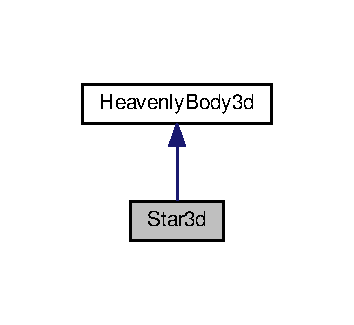
\includegraphics[width=170pt]{d0/dd1/classStar3d__inherit__graph}
\end{center}
\end{figure}


\-Collaboration diagram for \-Star3d\-:
\nopagebreak
\begin{figure}[H]
\begin{center}
\leavevmode
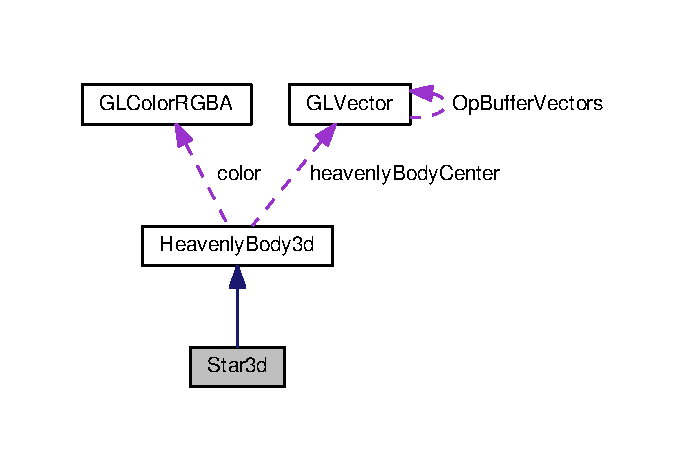
\includegraphics[width=331pt]{da/dcf/classStar3d__coll__graph}
\end{center}
\end{figure}
\subsection*{\-Public \-Member \-Functions}
\begin{DoxyCompactItemize}
\item 
\hyperlink{classStar3d_a2d09eb43e716f50254f12a6f0d5cd8f4}{\-Star3d} (\hyperlink{classHeavenlyBody}{\-Heavenly\-Body} $\ast$heavenly\-Body)
\begin{DoxyCompactList}\small\item\em \-Default constructor. \end{DoxyCompactList}\item 
void \hyperlink{classStar3d_a131a6612a83da74b25db2ff389e91424}{paint\-Heavenly\-Body3d} ()
\begin{DoxyCompactList}\small\item\em \-Paint the star without lighting effects. \end{DoxyCompactList}\end{DoxyCompactItemize}


\subsection{\-Detailed \-Description}
\-Class to paint the star of the solar system.

\begin{DoxyAuthor}{\-Author}
\-Fabian \-Deitelhoff $<$\href{mailto:FH@FabianDeitelhoff.de}{\tt \-F\-H@\-Fabian\-Deitelhoff.\-de}$>$ 

\-Christof \-Geisler $<$\href{mailto:christof.geisler@stud.fh-swf.de}{\tt christof.\-geisler@stud.\-fh-\/swf.\-de}$>$ 
\end{DoxyAuthor}


\subsection{\-Constructor \& \-Destructor \-Documentation}
\hypertarget{classStar3d_a2d09eb43e716f50254f12a6f0d5cd8f4}{
\index{\-Star3d@{\-Star3d}!\-Star3d@{\-Star3d}}
\index{\-Star3d@{\-Star3d}!Star3d@{\-Star3d}}
\subsubsection[{\-Star3d}]{\setlength{\rightskip}{0pt plus 5cm}\-Star3d\-::\-Star3d (
\begin{DoxyParamCaption}
\item[{{\bf \-Heavenly\-Body} $\ast$}]{heavenly\-Body}
\end{DoxyParamCaption}
)}}
\label{d2/d14/classStar3d_a2d09eb43e716f50254f12a6f0d5cd8f4}


\-Default constructor. 


\begin{DoxyParams}{\-Parameters}
{\em heavenly\-Body} & \\
\hline
\end{DoxyParams}

\begin{DoxyCode}
    : HeavenlyBody3d(heavenlyBody)
{
}
\end{DoxyCode}


\subsection{\-Member \-Function \-Documentation}
\hypertarget{classStar3d_a131a6612a83da74b25db2ff389e91424}{
\index{\-Star3d@{\-Star3d}!paint\-Heavenly\-Body3d@{paint\-Heavenly\-Body3d}}
\index{paint\-Heavenly\-Body3d@{paint\-Heavenly\-Body3d}!Star3d@{\-Star3d}}
\subsubsection[{paint\-Heavenly\-Body3d}]{\setlength{\rightskip}{0pt plus 5cm}void \-Star3d\-::paint\-Heavenly\-Body3d (
\begin{DoxyParamCaption}
{}
\end{DoxyParamCaption}
)\hspace{0.3cm}{\ttfamily  \mbox{[}virtual\mbox{]}}}}
\label{d2/d14/classStar3d_a131a6612a83da74b25db2ff389e91424}


\-Paint the star without lighting effects. 



\-Reimplemented from \hyperlink{classHeavenlyBody3d_a030592ed6fd43987d2b004f56a3ab3a8}{\-Heavenly\-Body3d}.


\begin{DoxyCode}
{
    glDisable(GL_LIGHTING);

    glColor3f(color.red(), color.green(), color.blue());

    HeavenlyBody3d::paintHeavenlyBody3d();

    glEnable(GL_LIGHTING);
}
\end{DoxyCode}


\-The documentation for this class was generated from the following files\-:\begin{DoxyCompactItemize}
\item 
visualization/heavenlybody/\hyperlink{star3d_8h}{star3d.\-h}\item 
visualization/heavenlybody/\hyperlink{star3d_8cpp}{star3d.\-cpp}\end{DoxyCompactItemize}

\printindex
\end{document}
